\documentclass[12pt,a4paper,twoside,english,final]{ETHthesis}

% !TEX root = main.tex
\usepackage{ETHthesis}
\usepackage[english]{babel}

% Fonts
\usepackage[T1]{fontenc}
\usepackage[utf8]{inputenc}
\usepackage{lmodern}
\usepackage[usenames, dvipsnames]{xcolor}
\usepackage[dottedtoc,floatperchapter,parts]{classicthesis}

% \usepackage[showframe]{geometry} # Useful to check hbox issues
\usepackage{amsmath, amssymb, amsthm}

% Biblio
\usepackage{csquotes}
\usepackage[backend=bibtex,
            style=alphabetic, natbib=true, url=false,
            isbn=false, backref=true, maxcitenames=3,
            maxbibnames=35]{biblatex}

\usepackage[labelfont=bf]{caption}
\usepackage{subcaption}
\usepackage{tikz}
\usepackage{bbm}
\usepackage{dsfont}
\usepackage{mathtools}
\usepackage{graphicx}

% Tables
\usepackage{tabularx}
\usepackage{booktabs}

% Algorithms
\usepackage[noend]{algpseudocode}
\usepackage{algorithm,algorithmicx}
\usepackage{eqparbox}
\usepackage{xspace}

\usepackage{enumitem}
\setlist[enumerate]{leftmargin=*}

\usepackage{titlesec}
\usepackage{hyperref}
\hypersetup{pdfauthor={Mikhail Karasikov}, pdftitle={}, pdfsubject={A thesis submitted to attain the degree of Doctor of Sciences to ETH Zurich},
            pdflang={en}, bookmarksnumbered, pageanchor=true, plainpages=false, colorlinks=true, linktocpage=true,
            citecolor=MidnightBlue, filecolor=BrickRed, linkcolor=NavyBlue, urlcolor=ForestGreen}

\definecolor{light-gray}{gray}{0.65}
\titleformat{\chapter}% Command
[display]% shape
{\bfseries\Large}% Format for the whole title
{\filleft{\fontsize{80}{100}\selectfont\color{light-gray}\thechapter}}% Label
{-25pt}% horizontal separation (vertical for display)
{\filleft\fontsize{26}{35}\selectfont}% Before Code
[\vspace{5pt}\titlerule]

%% Page Layout
\setlength{\topmargin}{-7.5mm}
\setlength{\headheight}{5mm}
\setlength{\headsep}{+12.5mm}
\setlength{\textheight}{220mm}
\setlength{\footskip}{+20.mm}
\setlength{\textwidth}{161mm} %!!!
\setlength{\parindent}{0pt}
\setlength{\parskip}{1ex plus 0.25ex minus 0.25ex}
\iftwoside
\setlength{\oddsidemargin}{3mm}
\setlength{\evensidemargin}{-3mm}
\else
\setlength{\oddsidemargin}{0mm}
\setlength{\evensidemargin}{0mm}
\fi
\raggedbottom

%% Float Placement
\renewcommand{\topfraction}{0.85}
\renewcommand{\bottomfraction}{0.85}
\renewcommand{\textfraction}{0.15}
\renewcommand{\floatpagefraction}{0.1}
\renewcommand{\baselinestretch}{1.15}

% Allow subsubsections to have numbers (and be references)
\setcounter{secnumdepth}{3}
% Allow subsubsections to appear in the TOC
\setcounter{tocdepth}{3}
% \setcounter{lofdepth}{2} % we want subfigures in the list of figures

%% Line spacing
\linespread{1.25}

%% Avoid Widows and Orphans
\widowpenalty=1000
\clubpenalty=1000

\vfuzz2pt % Don't report over-full v-boxes if over-edge is small
\hfuzz2pt % Don't report over-full h-boxes if over-edge is smallq

% !TEX root = main.tex
% Allow overfull boxes which don't overflow more than 20pts (remove before the last version)
\hfuzz=20pt

% Issue with transparency of included pdf images (if there is more than 1 per page with \group
% defined pdflatex doesn't know which one to consider the top one ...)
\pdfsuppresswarningpagegroup=1

\newcommand{\cleardoublepageempty}{
  \clearpage
  \thispagestyle{empty}
  \cleardoublepage
}

\usepackage{array}
\newcolumntype{H}{>{\setbox0=\hbox\bgroup}c<{\egroup}@{}} % Useful to hide a column of a table (just define it as H)

\newtheorem*{rep@theorem}{\rep@title}
\newcommand{\newreptheorem}[2]{%
\newenvironment{rep#1}[1]{%
 \def\rep@title{#2 \ref{##1}}%
 \begin{rep@theorem}}%
 {\end{rep@theorem}}}
\newreptheorem{lemma}{Lemma'}
\newreptheorem{theorem}{Theorem'}
\newreptheorem{corollary}{Corollary'}
\newtheorem{theorem}{Theorem}
\newtheorem{lemma}[theorem]{Lemma}
\newtheorem{corollary}[theorem]{Corollary}
\newtheorem{definition}[theorem]{Definition}
\newtheorem{proposition}[theorem]{Proposition}
\makeatletter
\@addtoreset{theorem}{chapter}
\makeatother

\newcommand{\mop}[1]{\mathop{\text{#1}}}

\makeatletter
\DeclareRobustCommand\bfseries{%
  \not@math@alphabet\bfseries\mathbf
  \fontseries\bfdefault\selectfont
  \boldmath % <-- added
}
\makeatother
% !TEX root = main.tex
\usepackage{url}            % simple URL typesetting
\usepackage{amsfonts}       % blackboard math symbols
\usepackage{nicefrac}       % compact symbols for 1/2, etc.
\usepackage{microtype}      % microtypography
\usepackage{amsbsy}%
\usepackage{calc}
\usepackage{moresize}
\usepackage{siunitx}
\usepackage{bm}
\usepackage{multirow}
\usepackage{printlen}
\newtheorem{assu}{Assumption}
\newtheorem{remark}{Remark}

\usepackage{multicol}
\usepackage{footmisc}
\usetikzlibrary{positioning, matrix, shapes,trees}
\usepackage{mathtools}
\usepackage[export]{adjustbox}
\usepackage{wrapfig}
\usepackage[outdir=./]{epstopdf}
\usepackage[sort=def]{glossaries}

% \usepackage{sistyle}
% \SIthousandsep{,}
%\usepackage{breqn}


\makeatletter
\makeatother

\usepackage{tikz}
\usetikzlibrary{calc}
\tikzset{mynode/.style={draw,circle, minimum size = 0.7cm}}
\usetikzlibrary{positioning,shapes,arrows}
\usepackage{xcolor}

\definecolor{gblue}{RGB}{207,226,243}
\definecolor{gred}{RGB}{244,204,204}
\definecolor{gyellow}{RGB}{255,229,153}
\definecolor{gyellow2}{RGB}{252,229,205}
\definecolor{ggreen}{RGB}{217,234,211}
\definecolor{ggray}{RGB}{238,238,238} 
\definecolor{ggray2}{RGB}{81,84,87} 
\definecolor{gpurple}{RGB}{217,210,233} 

\usepackage{anyfontsize}

% \usepackage{forest}
% \definecolor{folderbg}{RGB}{124,166,198}
% \definecolor{folderborder}{RGB}{110,144,169}
% \def\Size{4pt}
% \tikzset{
%   folder/.pic={
%     \filldraw[draw=folderborder,top color=folderbg!50,bottom color=folderbg]
%       (-1.05*\Size,0.2\Size+5pt) rectangle ++(.75*\Size,-0.2\Size-5pt);
%     \filldraw[draw=folderborder,top color=folderbg!50,bottom color=folderbg]
%       (-1.15*\Size,-\Size) rectangle (1.15*\Size,\Size);
%   }
% }

\usepackage{listings}

\usepackage{tabularray}

% !TEX root = main.tex

%%%%%%%%%%%%%%%%%%%%%%%%%%%%%%%%%%%%%%%%%%%%%%%%%%%%%%%%%%%%%%%%%%%%%%%%%%%%%%%
% Overall commands
%%%%%%%%%%%%%%%%%%%%%%%%%%%%%%%%%%%%%%%%%%%%%%%%%%%%%%%%%%%%%%%%%%%%%%%%%%%%%%%
% Comments
\newcommand{\FL}[1]{{\textcolor{blue}{{\bf FL:} #1}}}

% Common expressions
\newcommand{\ie}{\textit{i.e.}\xspace}
\newcommand{\eg}{\textit{e.g.}\xspace}
\newcommand{\iid}{\textit{i.i.d.}\xspace}

% Full citations
\makeatletter
\newcommand{\upmax}{\def\blx@maxcitenames{99}}
\newcommand{\dnmax}{\def\blx@maxcitenames{1}}
\makeatother
\newcommand{\myfullcite}[1]{\upmax\fullcite{#1}\dnmax}

%%%%%%%%%%%%%%%%%%%%%%%%%%%%%%%%%%%%%%%%%%%%%%%%%%%%%%%%%%%%%%%%%%%%%%%%%%%%%%%
% MAIN BACKGROUND
%%%%%%%%%%%%%%%%%%%%%%%%%%%%%%%%%%%%%%%%%%%%%%%%%%%%%%%%%%%%%%%%%%%%%%%%%%%%%%%

% Big-O notation
\newcommand{\Or}[1]{\mathcal{O}\mathopen{}\left(#1\right)\mathclose{}}
\newcommand{\OrTilde}[1]{\tilde{\mathcal{O}}\mathopen{}\left(#1\right)\mathclose{}}
\newcommand{\Th}[1]{\Theta\mathopen{}\left(#1\right)\mathclose{}}
\newcommand{\Om}[1]{\Omega\mathopen{}\left(#1\right)\mathclose{}}

\newcommand{\encase}[1]{{\left[#1\right]}}
\newcommand{\brac}[1]{{\left(#1\right)}}


% Real numbers
\newcommand{\R}{\mathbb{R}}
\newcommand{\N}{\mathbb{N}}

% Optimization notation
\newcommand{\trace}{\operatorname{tr}}
\newcommand{\dist}{\operatorname{dist}}
\newcommand{\norm}[1]{\Vert #1 \Vert}
\newcommand{\ip}[2]{\big\langle #1, \, #2 \big\rangle}
\newcommand{\prox}[1]{\mathrm{prox}_{#1}}
\newcommand{\proj}[1]{\mathrm{proj}_{#1}}
\newcommand{\lmo}{\textit{lmo}\xspace}
\def\bbE{{\mathbb{E}}}
\def\E{{\mathbb{E}}}
\def\sR{{\mathbb{R}}}
\def\sZ{{\mathbb{Z}}}

\DeclareMathOperator*{\argmin}{arg\,min}
\DeclareMathOperator*{\argmax}{arg\,max}

% Optimization problems
\DeclareMathOperator{\conv}{conv}
\DeclareMathOperator{\lin}{lin}
\DeclareMathOperator{\cone}{cone}

% VI Commands
\newcommand{\dkl}{D^{KL}}
\newcommand{\KL}{D^{KL}}
\newcommand{\relbo}{\textsc{RELBO}\xspace}


% Algorithms
\newcommand{\FW}{{\textsf{\tiny FW}}}


\DeclareMathOperator{\l1}{L1-ball}
\DeclareMathOperator{\Cf}{C_f}
\DeclareMathOperator{\radius}{\mathrm{radius}}
\DeclareMathOperator{\diam}{\mathrm{diam}}
\DeclareMathOperator{\mdw}{mDW(\cA)}
\DeclareMathOperator{\ama}{{\cA\cup-\cA}}
\DeclareMathOperator{\amx}{\left\lbrace\cA\cup-\frac{\theta_k}{\|\theta_k\|_\cA}\right\rbrace}
\DeclareMathOperator{\amxnok}{\left\lbrace\cA\cup-\frac{\theta}{\|\theta\|_\cA}\right\rbrace}
\DeclareMathOperator{\faces}{faces}
\DeclareMathOperator{\gfaces}{g-faces}
\DeclareMathOperator{\madw}{mADW(\cA)}
\DeclareMathOperator{\cw}{CWidth(\cA)}
\DeclareMathOperator{\clip}{clip}

% Matchal laetters
\def\cA{\mathcal{A}}
\def\cB{\mathcal{B}}
\def\cD{\mathcal{D}}
\def\cF{\mathcal{F}}
\def\cH{\mathcal{H}}
\def\cK{\mathcal{K}}
\def\cL{\mathcal{L}}
\def\cN{\mathcal{N}}
\def\cQ{\mathcal{Q}}
\def\cS{\mathcal{S}}
\def\cT{\mathcal{T}}
\def\cZ{\mathcal{Z}}

% Random Variables
\def\rva{{\mathbf{a}}}
\def\rvb{{\mathbf{b}}}
\def\rvc{{\mathbf{c}}}
\def\rvd{{\mathbf{d}}}
\def\rve{{\mathbf{e}}}
\def\rvf{{\mathbf{f}}}
\def\rvg{{\mathbf{g}}}
\def\rvh{{\mathbf{h}}}
\def\rvu{{\mathbf{i}}}
\def\rvj{{\mathbf{j}}}
\def\rvk{{\mathbf{k}}}
\def\rvl{{\mathbf{l}}}
\def\rvm{{\mathbf{m}}}
\def\rvn{{\mathbf{n}}}
\def\rvo{{\mathbf{o}}}
\def\rvp{{\mathbf{p}}}
\def\rvq{{\mathbf{q}}}
\def\rvr{{\mathbf{r}}}
\def\rvs{{\mathbf{s}}}
\def\rvt{{\mathbf{t}}}
\def\rvu{{\mathbf{u}}}
\def\rvv{{\mathbf{v}}}
\def\rvw{{\mathbf{w}}}
\def\rvx{{\mathbf{x}}}
\def\rvy{{\mathbf{y}}}
\def\rvz{{\mathbf{z}}}

\def\sfA{\mathsf{A}}
\def\sfQ{\mathsf{Q}}
\def\sfZ{\mathsf{Z}}

% Random variables
\def\reta{{\textnormal{$\eta$}}}
\def\ra{{\textnormal{a}}}
\def\rb{{\textnormal{b}}}
\def\rc{{\textnormal{c}}}
\def\rd{{\textnormal{d}}}
\def\re{{\textnormal{e}}}
\def\rf{{\textnormal{f}}}
\def\rg{{\textnormal{g}}}
\def\rh{{\textnormal{h}}}
\def\ri{{\textnormal{i}}}
\def\rj{{\textnormal{j}}}
\def\rk{{\textnormal{k}}}
\def\rl{{\textnormal{l}}}
% rm is already a command, just don't name any random variables m
\def\rn{{\textnormal{n}}}
\def\ro{{\textnormal{o}}}
\def\rp{{\textnormal{p}}}
\def\rq{{\textnormal{q}}}
\def\rr{{\textnormal{r}}}
\def\rs{{\textnormal{s}}}
\def\rt{{\textnormal{t}}}
\def\ru{{\textnormal{u}}}
\def\rv{{\textnormal{v}}}
\def\rw{{\textnormal{w}}}
\def\rx{{\textnormal{x}}}
\def\ry{{\textnormal{y}}}
\def\rz{{\textnormal{z}}}


\def\va{{\textbf{a}}}
\def\vb{{\textbf{b}}}
\def\vc{{\textbf{c}}}
\def\vd{{\textbf{d}}}
\def\ve{{\textbf{e}}}
\def\vf{{\textbf{f}}}
\def\vg{{\textbf{g}}}
\def\vh{{\textbf{h}}}
\def\vi{{\textbf{i}}}
\def\vj{{\textbf{j}}}
\def\vk{{\textbf{k}}}
\def\vl{{\textbf{l}}}
\def\vm{{\textbf{m}}}
\def\vn{{\textbf{n}}}
\def\vo{{\textbf{o}}}
\def\vp{{\textbf{p}}}
\def\vq{{\textbf{q}}}
\def\vr{{\textbf{r}}}
\def\vs{{\textbf{s}}}
\def\vt{{\textbf{t}}}
\def\vu{{\textbf{u}}}
\def\vv{{\textbf{v}}}
\def\vw{{\textbf{w}}}
\def\vx{{\textbf{x}}}
\def\vy{{\textbf{y}}}
\def\vz{{\textbf{z}}}

% Matrix
\def\mA{{\textbf{A}}}
\def\mB{{\textbf{B}}}
\def\mC{{\textbf{C}}}
\def\mD{{\textbf{D}}}
\def\mE{{\textbf{E}}}
\def\mF{{\textbf{F}}}
\def\mG{{\textbf{G}}}
\def\mH{{\textbf{H}}}
\def\mI{{\textbf{I}}}
\def\mJ{{\textbf{J}}}
\def\mK{{\textbf{K}}}
\def\mL{{\textbf{L}}}
\def\mM{{\textbf{M}}}
\def\mN{{\textbf{N}}}
\def\mO{{\textbf{O}}}
\def\mP{{\textbf{P}}}
\def\mQ{{\textbf{Q}}}
\def\mR{{\textbf{R}}}
\def\mS{{\textbf{S}}}
\def\mT{{\textbf{T}}}
\def\mU{{\textbf{U}}}
\def\mV{{\textbf{V}}}
\def\mW{{\textbf{W}}}
\def\mX{{\textbf{X}}}
\def\mY{{\textbf{Y}}}
\def\mZ{{\textbf{Z}}}

\def\gA{{\mathcal{A}}}
\def\gB{{\mathcal{B}}}
\def\gC{{\mathcal{C}}}
\def\gD{{\mathcal{D}}}
\def\gE{{\mathcal{E}}}
\def\gF{{\mathcal{F}}}
\def\gG{{\mathcal{G}}}
\def\gH{{\mathcal{H}}}
\def\gI{{\mathcal{I}}}
\def\gJ{{\mathcal{J}}}
\def\gK{{\mathcal{K}}}
\def\gL{{\mathcal{L}}}
\def\gM{{\mathcal{M}}}
\def\gN{{\mathcal{N}}}
\def\gO{{\mathcal{O}}}
\def\gP{{\mathcal{P}}}
\def\gQ{{\mathcal{Q}}}
\def\gR{{\mathcal{R}}}
\def\gS{{\mathcal{S}}}
\def\gT{{\mathcal{T}}}
\def\gU{{\mathcal{U}}}
\def\gV{{\mathcal{V}}}
\def\gW{{\mathcal{W}}}
\def\gX{{\mathcal{X}}}
\def\gY{{\mathcal{Y}}}
\def\gZ{{\mathcal{Z}}}


\renewcommand{\P}{P}
\newcommand{\Q}{Q}

\DeclareRobustCommand{\myhammer}{%
  \begingroup\normalfont
  \includegraphics[height=1.1\fontcharht\font`\B]{sections/disent/figures/hammer.pdf}%
  \endgroup
}
\newcommand{\PA}{\textbf{PA}}
\newcommand{\supp}{\operatorname{supp}}

\newcommand\blfootnote[1]{%
  \begingroup
  \renewcommand\thefootnote{}\footnote{#1}%
  \addtocounter{footnote}{-1}%
  \endgroup
}


\newcommand{\softmax}[1]{\texttt{Softmax}\,(#1)}
\newcommand{\dotp}[1]{\texttt{dot}\,(#1)}
\newcommand{\reducesum}[1]{\texttt{reduce\_sum}\,(#1)}
\newcommand{\gru}[2]{\texttt{GRU}\,(#1, \ #2)}
\newcommand{\slots}[0]{\texttt{slots}}
\newcommand{\attn}[0]{\texttt{attn}}
\newcommand{\inp}[0]{\texttt{inputs}}
\newcommand{\mlp}[0]{\texttt{MLP}}
\newcommand{\sam}[0]{Slot Attention\xspace}
\newcommand{\w}[0]{\texttt{w}}
\newcommand{\updates}[0]{\texttt{updates}}
\newcommand{\layernorm}[0]{\texttt{LayerNorm}}
\newcommand\myeq{\mkern0.5mu{=}\mkern6mu}
% \renewcommand{\algorithmiccomment}[1]{#1}

\DeclareMathOperator{\rank}{rank}
\DeclareMathOperator{\select}{select}
\newcommand{\kmer}{\operatorname{\text{k-mer}}}

\makeatletter\renewcommand{\ALG@beginalgorithmic}{\small}\makeatother
\newcommand*\Let[2]{#1 $\gets$ #2}
\algnewcommand{\LineComment}[1]{\State \(\triangleright\) #1}
\algrenewcommand\algorithmicrequire{\textbf{Precondition:}}
\algrenewcommand\algorithmicensure{\textbf{Postcondition:}}
% declaration of the new block
% \algblock{ParFor}{EndParFor}
% customising the new block
% \algnewcommand\algorithmicparfor{\textbf{parfor}}
\algnewcommand\algorithmicpardo{\textbf{do}}
% \algnewcommand\algorithmicendparfor{\textbf{end\ parfor}}
% \algrenewtext{ParFor}[1]{\algorithmicparfor\ #1\ \algorithmicpardo}
% \algrenewtext{EndParFor}{\algorithmicendparfor}

% declaration of the new block
\algblock{ParForAll}{EndParForAll}
% customising the new block
\algnewcommand\algorithmicparforall{\textbf{for all}}
\algnewcommand\algorithmicparforalldo{\textbf{parallel do}}
\algrenewtext{ParForAll}[1]{\algorithmicparforall\ #1\ \algorithmicparforalldo}
\algtext*{EndParForAll}%

\def\code#1{\texttt{#1}}


\bibliography{thesis.bib}

\begin{document}
\initETHthesis

%%%%%%%%%%%%%%%%%%%%%%%%%%%%%%%%%%%%%%%%
% COVER PAGE %
%%%%%%%%%%%%%%%%%%%%%%%%%%%%%%%%%%%%%%%%
\dissnum{$000000$}
\title{Learning to align single-cell populations}
\author{Stefan G. Stark}
\acatitle{\normalsize M.Sc. in Computer Science,\\ETH Zurich}
\dateofbirth{March $11$, $1992$}
\citizen{United States}
\Year{2024}
\examiners{
	\normalsize
  Prof.\ Dr.\ Gunnar R\"atsch, examiner\linebreak
  Dr.\ Kjong-van Lehmann, examiner\linebreak
  Prof. Dr.\ Andreas Krause, co-examiner\linebreak
  Prof. Dr.\ Oliver Stegle, co-examiner\linebreak
}
\support{}
\disclaimer{}
\pagestyle{empty}
\hypersetup{pageanchor=false}
\maketitle
\hypersetup{pageanchor=true}

%%%%%%%%%%%%%%%%%%%%%%%%%%%%%%%%%%%%%%%%
% PREAMBLE %
%%%%%%%%%%%%%%%%%%%%%%%%%%%%%%%%%%%%%%%%
\pagestyle{plain}
\pagenumbering{roman}
% !TeX root = ../main.tex

\pdfbookmark[1]{Abstract}{Abstract}
\begingroup
\let\clearpage\relax
\let\cleardoublepage\relax
\let\cleardoublepage\relax

\chapter*{Abstract}
Cellular states are complex -- their underlying genomic sequence, RNA transcription levels, accessibility of chromatin regions, protein levels, chemical activity, etc, work in tandem to determine the behavior of a cell and its responses to changes in its environment. 
Initially, the study of cellular populations relied on bulk profiling technologies
%which average individual cellular signals across population into a single observation, and
that made it difficult to study heterogeneous populations.
However, this last decade has seen, and continues to see, an explosion in the development of single-cell profiling technologies that allow individual cellular states to be observed at scale.
While these technologies revolutionized the study of cellular biology, they are still typically limited in the sense that they consume or otherwise destroy profiled cells.
This means that an individual cell can only be measured once.
As a result, these technologies are only able to measure projections of the underlying \textit{holistic} cellular state into a single observable domain, measuring, for instance, either a cell's RNA transcript abundance or the protein levels.
Furthermore, modeling temporal processes, such as perturbation responses, remain challenging, as these complex behaviors must be recovered without access to some set of paired "input-output" states.

This thesis is broadly concerned with the development and application of machine-learning based methods to reconcile this single-observation limitation.
The typical modern single-cell experiment will generate two (or more) datasets, which we can consider sampled from distributions over cellular states, $\mu$ and $\nu$, that share some non-trivial relationship.
We aim to recover this relationship by learning to \emph{align} these cellular populations.
Specifically we describe how to
i) integrate multi-modal observations, in which $\mu$ and $\nu$ represent the state of population different observable domains
and ii) model perturbation responses of cellular populations, in which $\mu$ and $\nu$ represent population state at two different time points.
A major theme throughout this thesis is the demonstration of clinical utility of the developed methods.
In particular, we apply a method developed to recover and predict heterogeneous single-cell responses to a cohort of melanoma patients and demonstrate how it can improve the analysis, understanding, and ultimately help tailor their treatments.




\newpage
\begin{otherlanguage}{ngerman}
\pdfbookmark[1]{Zusammenfassung}{Zusammenfassung}
\chapter*{Zusammenfassung}
% TODO: (later) translate abstract
[german translation]
\end{otherlanguage}


%\newpage
%\chapter*{Acknowledgments}
% TODO: (later) write awks
\endgroup

\vfill

\cleardoublepageempty{}
\selectlanguage{english}

%%%%%%%%%%%%%%%%%%%%%%%%%%%%%%%%%%%%%%%%
% TOC %
%%%%%%%%%%%%%%%%%%%%%%%%%%%%%%%%%%%%%%%%
\setlength{\cftbeforechapskip}{4mm}
\setcounter{tocdepth}{1}
\pagestyle{myheadings}
\pdfbookmark[0]{\contentsname}{contents}
\tableofcontents
\cleardoublepageempty{}

%%%%%%%%%%%%%%%%%%%%%%%%%%%%%%%%%%%%%%%%
% GLOSSARY %
%%%%%%%%%%%%%%%%%%%%%%%%%%%%%%%%%%%%%%%%
%\printnoidxglossaries
%\cleardoublepageempty{}

%%%%%%%%%%%%%%%%%%%%%%%%%%%%%%%%%%%%%%%%
% BODY %
%%%%%%%%%%%%%%%%%%%%%%%%%%%%%%%%%%%%%%%%
% TODO: pass over all section titles
\pagenumbering{arabic}
\cleardoublepageempty{}
% !TeX root = ../main.tex

\chapter{Introduction}

%\subsection{Scope}
% TODO: (optional) write scope
%\subsection{Publications}
% TODO: (optional) write pubs
%\subsection{Collaborators}
% TODO: (optional) write collabs

\section{Individual cells as complex machinery}
Cells are the basic building block of life -- all living organisms are composed of one or more cells.
They can be considered as complex machines engineered over billions of years of evolution,
which have resulted in intricate cellular "programs" that determine the identify, behavior, and interactions of cells with each other and their environments.
These programs perform a wide range of functions necessary for life, including metabolism, growth, reproduction, response to stimuli, and adaptation to environment.

Recent technological advances in single-cell biology have revolutionized the way scientists are able to study cells.
The development of \emph{single-cell profiling technologies} enable measurements at the resolution of individual cells,
promising a better understanding of cellular development and interaction, with particular implications in the study of cancer.
This data is quite difficult to analyze, as reflected by the underlying complexity of cellular biology, and
computational tools have proven to play an important role in unlocking the full potential of these technologies.
This thesis is largely concerned with the development as well as application of such machine-learning based computational tools to problems tackled with single-cell profiling technologies.

The goal of this chapter is to give a high level introduction to the basics of cellular biology in order to properly motivate the context and intracies of the single-cell data within this thesis.
The hope here is that it useful for readers with a non-biological background, such as those coming from a machine learning field that who would like to gain a better understanding of the powers underneath their data.

\subsection{The central dogma of biology}
At the core of each cell's identity is the \emph{genetic code}, a long sequence encoded biologcally as DNA molecules.
This code acts as a "blueprint" for cellular processes and
is replicated and propogated as part of the cellular life cycle.
While the genetic information of cells within an individual human (or another complex multi-cellular organism) is essentially conserved, their cells take on a myriad of different forms and functions.
For instance, different \emph{cell types} -- skin cells, red blood cells, liver cells, nerve cells, etc -- within an individual all share the same genetic information despite exhibiting vastly different appearances and roles.
Thus, not just the content of the genetic code, but how the genetic code is processed plays a critical role in determining the cell.

The \emph{central dogma} is a paradigm that describes this process of extracting genetic information.
Cellular behavior is driven in large part by protein molecules which exert influence through chemical interactions within their inter- and intra-cellular environments.
In essence, proteins are one-dimensional sequences of twenty distinct organic compounds known as amino acids and are constructed from interpretation of the genetic code.
On a high level, genes, particular sections of the genetic code stored in the form DNA, are transcribed into a corresponding RNA molecule, which are then translated into some specific protein.
While the reality is more complicated, the information flow generally flows from DNA to RNA to proteins.

An overview of the essential characteristics of each level in the central dogma is given below:

\paragraph{DNA} The genetic code is stored in the form of DNA (dioxyribose nucelic acid) molecules.
These long polymer chains are sequences of only four unique monomers called nucleotides.
When a cell divides, its DNA is replicated such that the daughter cells are composed of identical copies of the genetic code.
As DNA forms the base of the central dogma, the root of the information flow, it is important that its makeup is conserved.
While DNA famously exhibits a double-stranded helical structure,
each nucleotide has a unique corresponding partner whose bonds connect the two strands.
The genetic code, as represented by DNA, is often regarded as a one-dimensional string.
This double-stranded structure represents a redundancy in information and is exploited by cellular processes aimed at conserving the integrity of the genetic code.
Furthermore, in eukaryotic cells, from which all multi-cellular organisms (fungi, plants, and animals) are comprised, DNA is stored within the nucleus of the cell.
The nucleus protects the DNA with its own membrane that regulates the flow of chemical entities in and out of it and the DNA itself generally does not leave the nucleus \cite{milo2015}.

\paragraph{RNA} RNA (ribonucleic acid) is the intermediate step in the central dogma and plays a central in gene expression and regulation.
Since DNA is typically secured and isolated from interacting with the cellular environment, RNA can be understood as its intermediary.
RNA is constructed in a process called \emph{transcription}, where DNA is unwound and converted into RNA.
Like DNA, RNA is composed of a sequence of four unique nucleotides, which are the same as DNA except that thymine (T) is replaced with uracil (U).
In a processes called \emph{translation}, RNA strands are read to create specific proteins.
In this way, RNA plays the central role in gene expression, determining what proteins are created as well as the rate of their creation.
As the cells of a single organism share the vast majority of their DNA, 
gene expression is what allows them to differentiate and specialize.
Gene expression is also used to understand what processes the cell activates or de-activates due to changes in its environment.

\paragraph{Proteins} Proteins represent the ultimate stage of the central dogma and are largely responsible for the behavior and general function of a cell.
Like DNA and RNA, proteins can be conceptualized as one-dimensional sequences over an alphabet of twenty \emph{amino acids}.
During translation, this amino acid sequence is read from the genetic code where triplets of RNA nucleotides are converted into a single amino acid.
Proteins, however, have complicated 3D shapes that are fundamentally tied to its functions.
In a process known as \emph{protein folding}, chemical interactions between a protein's amino acids cause it to contort, yielding these complicated 3D structures.
Hemoglobin, for instance, a protein found in red blood cells that plays a critical role in the transport of oxygen, has a 3D shape that interacts chemically with oxygen molecules in order to absorb and release them.

\subsection{Pathways and cellular signaling}
Cellular processes are controlled and executed, in large part, via signals to proteins encoded as chemical interactions
While the 3D form of a protein largely determines its function,
these forms are not static and can change,
either through the breaking and reforming of bonds between a protein's amino acids,
or through the binding of some external chemical object.
Returning to the example of oxygen transport by hemoglobin -- the function of hemoglobin is to i) bind oxygen in the lung and ii) release it throughout the body.
Hemoglobin has two stable conformations that favor either the capture or release of oxygen molecules.
The preferred conformation is driven by chemical interactions determined by pH and oxygen concentration of the environment \cite{riggs1971}.

A common form of cellular signaling occurs when a protein and some external chemical object interact through the formation of chemical bonds.
An entity that binds to a protein is called a ligand and these ligands can range in complexity from simple ions to entire proteins.
Protein-ligand interactions are complex and are typically made with multiple bonds across many amino acids within the protein, often in the form of some "pocket" or "cavity" within the protein's 3D shape.
Resulting from this complexity, proteins have a high specificity for ligand binding and are usually only able to interact with few ligands.
Ligand binding can, for instance, change or stabilize a protein's shape, influence its chemical properties, form multi-protein complexes, etc, thus changing its shape and therefore function.

Major cellular processes, interactions, and responses are governed through complex and highly regulated signaling hierarchies called \emph{pathways}.
These pathways are composed of, typically, dozens of proteins that illicit cellular response through the capturing and relaying of chemical signals from the external cellular environment into the cellular interior.
Signaling within these pathways is often carried out through ligand binding that can \emph{activate} or \emph{deactivate} proteins, i.e. change their properties such that they included or excluded from participating in some cellular action.
Pathways govern fundamental cellular decisions, for instance, dictating how and when to grow, divide, differentiate, die, etc.
These decisions are typically enacted through the activation (or deactivation) of some key protein, or by ordering the transcription and translation of some specific gene.
Figure \ref{fig:hallmarks} depicts the general structure of a signaling pathway and a cartoon of the MAPK-ERK pathway, a pathway essential to regulating cell growth.

% TODO: (later) adapt figure better
\begin{figure}
  \begin{center}
  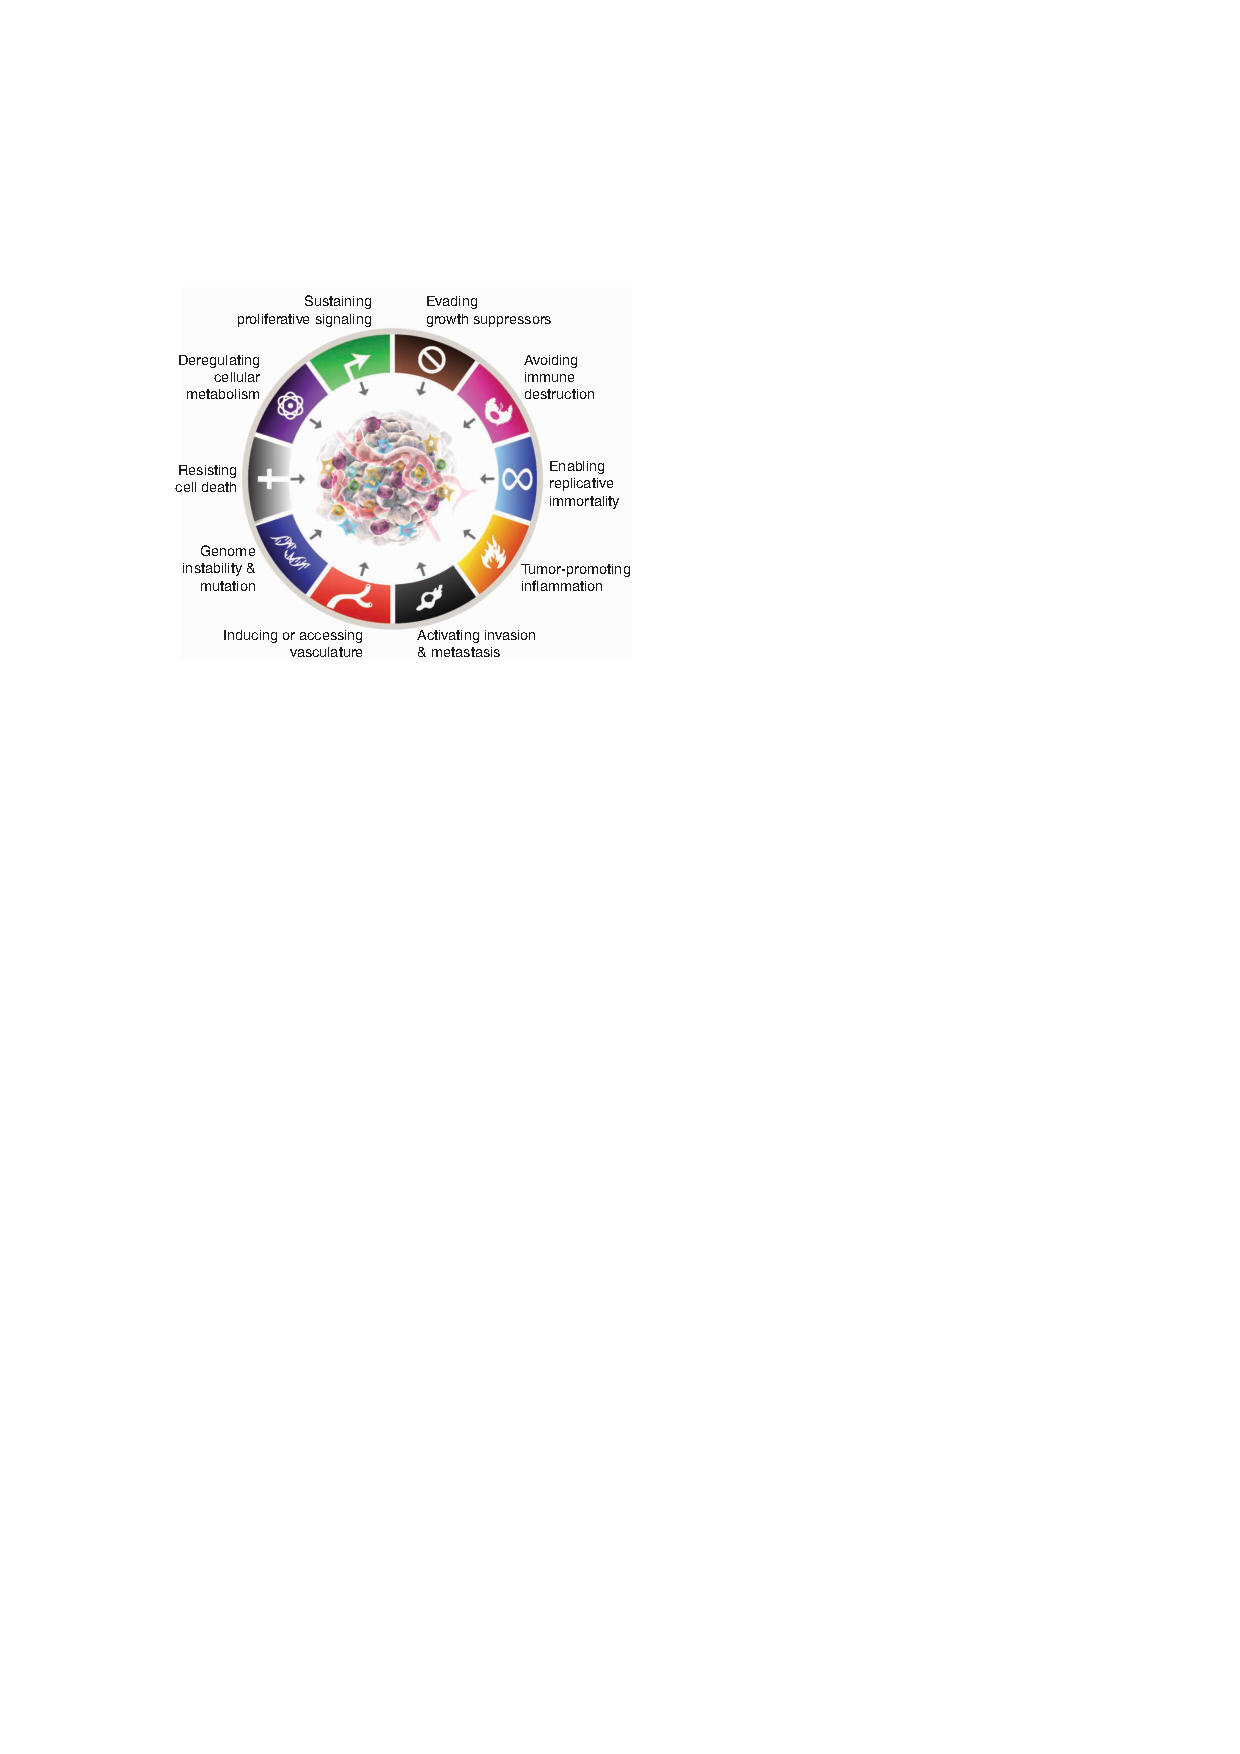
\includegraphics[width=0.95\textwidth]{figures/introduction/hallmarks.pdf}
  \end{center}
  \caption{Hallmarks of cancer, adapted from \cite{hanahan2011}}
  \label{fig:hallmarks}
\end{figure}


\paragraph{Centralized pathway databases}
Centralized databases of cellular signaling pathways are important resources to the biological research community.
These databases are curated through a combination of manual curation, literature reviews, and computational approaches, and distill the last few decades of cell biology research.
Reactome \cite{vastrik2007} and the Molecular Signatures Database (MSigDB) \cite{liberali2014} are two prominent centralized databases of cellular signaling pathways.
Reactome is a curated database of human biological pathways, including metabolic, signaling, and disease pathways.
It provides a comprehensive view of cellular processes and their interconnections.
MSigDB is a collection of gene sets expertly curated and automatically generated that represent a wide range of biological processes and signaling pathways.
Their "Hallmark" gene set contains a refined set of 50 pathways that represent essential gene functions.
These databases are widely used for pathway analysis, gene set enrichment analysis, and network analysis to understand cellular responses to different stimuli.
Other prominent databases in this field include KEGG \cite{kanehisa2000}, Biocarta \cite{nishimura2001}, and WikiPathways \cite{agrawal2024}.
These resources are crucial for understanding cellular signaling and identifying key regulators of biological processes.

\subsection{Genotype, phenotype, and mutations}
A useful abstraction is the distinction between an organisms's \emph{genotype}, the full set of information contained in its genetic code, and its \emph{phenotype}, its observable characteristics.
As we have seen, this relationship is far from one-to-one -- there are many factors beyond the genetic sequence that regulate and influence processes like transcription and translation.
However, it can happen that \emph{mutations}, changes in the genetic sequence, produce drastic effects on the phenotype.
For example, while redundancies exist between the 64 unique nucleotide triplets and the 20 unique amino acids they code for, changes to genetic code can sometimes cause a different amino acid to be translated.
If this change occurs within some important location within the protein, such as one critical to its shape or structure of a ligand binding site, the intended function of the protein can be invalidated.
Returning again to hemoglobin, the genetic disorder sickle-cell anemia is caused by a point mutation, a single nucleotide change in the genetic code, that alters the shape of the protein such that it cannot bind oxygen, to devastating effect.
As we will see, mutations play a critical role in the development of cancer, albeit in more nuanced and/or complicated contexts.

\section{Hallmarks of Cancer}
Cancer is a family of genetic diseases in which normal cells exhibit abnormal behavior that causes them to grow and proliferate uncontrollably, resulting in a mass of cells known as a tumor.
This growth can lead to serious health complications as cells
can then invade nearby tissues and spread to other parts of the body.
Over the last few decades, the development of effective cancer treatment strategies has been at the forefront of biomedical research and has been the focus of moonshots \cite{thewhitehouse2016} and large international consortia \cite{icgc2020}.
Despite this, cancer has remained an active research environment, challenging researchers to understand and control complex and nuanced cellular behaviors that can often times be specific to the tumor.
Many of the methods developed and applications explored within this thesis are motivated by challenges arising from understanding and treating cancer.

A major complication towards the treatment of cancer lie in the myriad mechanisms cells can use to escape the natural regulatory processes that prevent unchecked growth.
The \emph{Hallmarks of Cancer}, proposed by \citet{hanahan2000} in \citeyear{hanahan2000} and updated in \citeyear{hanahan2011} \cite{hanahan2011} and \citeyear{hanahan2022} \citep{hanahan2022}, is a framework to understand the key capabilities and enabling characteristics of cancer cells.
The framework (Figure \ref{fig:hallmarks}) describes eight capabilities, which can be considered as something akin to "gates" in the sense that they each represent some core regulatory process that must be bypassed in order for a normal cell to become cancerous, a process known as tumorigenesis.
In addition, the framework also describes two enabling characteristics, "Genome instability \& mutation" and "Tumor-promoting inflammation", which describe the general mechanisms used to bypass each "gate" and obtain the property of each hallmark characteristic.
In essence, the framework poses that in order for a cell to become a cancer cell, it must, by way of genetic mutations and tumor-promoting inflammation, both
i) sustain, promote, or generate cell growth signals, and, simultaneously,
ii) ignore or resist growth suppression or death (apoptosis) signals \cite{hanahan2011}.

\subsubsection{Genome instability \& mutations}
Genetic mutations are one of the underlying causes that enable cells to gain hallmark capabilities.
These "hallmark-granting" mutations typically change the coding of specific proteins key to cellular regulation.
As a result, these proteins become composed of slightly different amino acids and their shape and therefore function are changed.
This can cause gain or loss-of function, resulting in abnormal activation or deactivation of important cellular pathways.
Mutations in genes coding for these proteins are known as \emph{driver} mutations, as they take some of the core responsibility of guiding or driving tumorigenesis \cite{martinez-jimenez2020}.
identifying and then interrupting or reversing the effects of these driver mutations is a central strategy in cancer treatment.

Mutations in the BRAF gene are one of the most infamous examples of driver mutations.
Cell growth and proliferation are normal aspects of the cell life cycle.
In healthy cells, the signals that govern these processes are well regulated such that normal functions are maintained.
A signature property of cancer cells, on the other hand, is to deregulate these sources, resulting in abnormally high growth signals.
Changes to the BRAF protein, a key member of the RAS/MAPK signaling pathway \cite{davies2011}, a major intracellular signaling cascade that regulates cellular growth and proliferation,
can result in sustained growth-promoting signals.
Around 40\% of human melanomas contain a mutation in the BRAF gene, and 
85\% of these mutations are within the V600E subunit \cite{spathis2019}.
Consequently, many resources have been allocated towards the understanding of this protein, its common mutations \cite{smiech2020}, and treatment strategies \cite{cheng2018}.

Another class of driver mutations occur in so-called "tumor suppressor genes."
These genes code for proteins that are key members of the body's natural regulatory function that detect cancerous abnormalities and, in response, send growth-inhibiting signals \cite{joyce2024}.
Cancer cells must evade or ignore these signals in order to continue to grow unchecked,
typically by interrupting the pathways activated by these signals.
Mutations that interrupt the basic duties of these genes can be particularly harmful.

Mutations can be classified into one of two classes:
\emph{germline} mutations that are inherited and present at birth, or
\emph{somatic} mutations that are acquired throughout one's lifetime, e.g. by smoking, exposure to UV radiation, or simple random chance \cite{hanahan2011}.
A complication towards robust cancer treatments stems from the fact that individuals will have unique mutation combinations and the development of "one-size-fits-all" treatments are difficult or impossible.
Futhermore, while driver mutations appear in some subset of genes, they can affect different subunits and/or have different effects on the proteins downstream behavior \cite{smiech2020}.

As tumor cells proliferate, they copy and propagate their genetic mutations.
Tumor "clones" are genetically (and phenotypically) distinct cancer cells, arising from some original cancer cell.
Cancer cells, when compared to normal cells, are typically more susceptible to acquiring somatic mutations, due to, for instance, mutations in DNA-repair mechanisms \cite{negrini2010,salk2010}.
As a result, the genetics of cancer cells can exhibit a branching process within tumor clones, resulting what are known as tumor subclones.
The presence of these subclones represents a further complication in effective cancer treatment as these are not only specific to the individual but treatments need to address all active subclones which may exhibit differential responses to therapies.

\subsection{Inflammation and the tumor microenvironment}
Inflammation refers to an organism's natural biological response to harmful stimuli,
for instance, the immune system response to a foreign disease.
While it has been known that immune cells interact with and are involved in tumor formation, research over the last few decades has indicated that these interactions are crucial to the behavior of the tumor \cite{grivennikov2010, quail2013}.
This has lead to a sea-change in basic models of cancer -- tumors are not some relatively homogeneous mass of cancer cells experiencing unchecked growth, but a complex orchestra of interacting cells.
Under this tumor microenvironment (TME) model, tumors can be understood as something not unlike an organ that survives and propagates thanks to complex signaling interactions between many different cell types \cite{balkwill2012}, which are, as described above, specific to the individual.
Specifics of the TME have been shown to contribute to immune evasion \cite{pansy2021},
immunospression \cite{balta2021}, and immune cell reprogramming \cite{cao2022}.
It has also been shown that the immune responses within the TME can have 
have the counter-intuitive effect of \emph{promoting} tumor development \cite{hanahan2011}, for instance by supplying factors that promote growth \cite{denardo2010}.

%While the TME is not directly addressed within this thesis it is important to appreciate the underlying sources of tumor heterogeneity that must be captured by methods.
%Emerging spatial transcriptomic technologies \cite{need,need}, capable of measuring, for example, gene expression spatially-resolved at the single-cell level,
%have been shown to be promising directions towards the understanding of the TME \cite{need}.

\subsection{Strategies for treating cancer}
Common strategies to combat cancer usually involve blocking or reversing the specific mechanisms that enable critical hallmark capabilities.
Since the mutations and TME that drive the cancer hallmark capabilities can be unique to the individual,
developing a sweeping, generalized treatment to cancer is difficult.
Instead treatments are typically \emph{personalized} to the distinct mechanisms underlying each tumor.
There are two main approaches to treating cancer:
immunotherapy, which bolster the host immune system to identify and eliminate cancer cells,
and chemotherapy, which target and attack the cancer cells themselves \cite{hanahan2011}.

A class of chemotherapy comes in the form of orally ingested drugs that are designed to interact with specific pathways affected by cancerous mutations.
\emph{Targeted} therapies are a subclass of these chemotherapies that are designed for specific driver mutations.
For instance, the drug dabrafenib targets mechanisms underlying BRAF mutated cancer cells by inhibiting the activity of the BRAF V600E protein \cite{khunger2018}.
In general, these treatments can be conceptualized as perturbations over the heterogeneous makeup of a tumor, in which cells can have differential responses depending on their states, subclones, microenvironment, etc.
Combination therapies are another common strategy where two or more drugs are prescribed that either have synergistic effects or target multiple hallmark capabilities.
This strategy has been shown to be effective across multiple subclones, to bolster a targeted therapy, or to combat aggressive cancers \cite{hanahan2011}.

\section{Single-cell profiling technologies}
%\begin{enumerate}
%  \item even with the simplified view described here, there many information levels that determine cellular behavior
%  \item first advances into studying cell behavior, microscopes, hooke
%  \item nowadays, many technologies exist, taking different profiles of cells, different persepectives, etc
%  \item sequencing vs imaging vs whatever cytof is? 
%\end{enumerate}

Even with the simplified views described here, there are many levels of information -- e.g. DNA, RNA, protein -- that determine and govern cellular behavior.
As consequence, observations made on cells can come in many different forms and flavors that depend on the information or mechanisms of interest.
Omics refers to the some sub-field of cellular biological, typically ending with -omics, that studies some specific level of cellular information.
For instance,
genomics is the study of the complete set of genes in an organism,
transcriptomics is the study of RNA transcripts,
proteomics is the study of proteins,
but also
metabolomics is the study of metabolites,
epigenomics is the study of epigenetic modifications,
and so on.
Nowadays many strategies and technologies have been developed to measure and construct different cellular profiles, at the resolution of individual cells.
Each of these omics require the development of techniques and technologies specific to its profiling.
Within this thesis, methods are developed and applied primarily to transcriptomic and proteomic data.
The relevant technologies and data are described below.

%The measurement of proteomic information has a wider range of approaches, including fluorescent-based imaging and mass spe

\subsection{Transcriptomic profiling with scRNA-seq}
Genetic and transcriptomic information is measured with (single-cell) sequencing technologies that extract fragments of DNA/RNA and identify the sequences of nucleotides 
using so-called sequencing technologies.
These technologies are rooted in the Human Genome project,
a monumental scientific achievement that laid groundwork with the development of "next-gen" sequencing technology.
The human genome contains billions of nucleotides and so measuring this sequence end-to-end is infeasible.
Next gen sequencing technologies instead isolate and measure the nucleotide sequence of small fragments called reads.
The human genome project demonstrated how to assemble a genome, that is piece together the full sequence from overlapping fragments, like a colossal jigsaw puzzle \cite{lander2001}.
While the genome of each individual is distinct, the vast majority is conserved,
so, given some population of individuals, a \emph{reference} genome can be constructed to represent some average or canonical member of the population.
Once a reference is constructed, instead of assembling the code of a new individual from scratch, reads can then be \emph{mapped} onto the reference.

Whereas the human genome project was concerned with the measurement of genomic information,
the measurement of transcriptomic information, i.e. the nucleotide sequences of the free-floating RNA within a cell, follows the same general strategy.
Transcriptomic states are of particular interest as they represent something like a "real-time" snapshot of a cell's current actions.
Bulk sequencing technologies were the first iteration of technologies to measure cellular RNA states.
These technologies pool cells from a heterogeneous multi-cellular sample,
extract the RNA of individual cells, and measure a single signal that represents a composite of RNA states across all cells in the sample.
These technologies offer cheaper but low-resolution profiles, as the information from the individual are grouped together.
Deconvolution methods applied to a population of bulk measurements are popular approaches to infer higher resolution measurements, such as cell-type "signatures".
This approach is still quite limited as they rely on cell states that are conserved across many individuals in the population and we have seen,
such as in the case of cancer, that cellular behavior can be unique to the individual.

The last decade has seen, and continues to see, the development of single-cell sequencing technologies
that have revolutionized our capability to study cellular behaviors and especially in the context of heterogeneity \cite{moty2014}.
These technologies are capable of mechanically isolating individual cells and then sequencing its expressed RNA.
Instead of a single measurement over a sample, single-cell sequencing methods produce observations in the form of large count matrices of cells -x- genes,
where counts refer to the number of reads found in a cell that map to one of its genes.
For reference, humans have on the order of 20k protein coding genes.
While these methods offer deep insight into the inner workings of an individual cell, they must do so at the cost of much less transcriptomic information.
Single-cell technologies rely on a processing step in which successfully captured reads are first replicated before aligned.
The failure rates associated with capturing and replicating reads are thought to cause a "dropout" effect, where the single-cell observation fails to detect genes that are actually expressed.
However, it is understood that, at any given time, cells may express only a small subset of their total genes \cite{adams2008}.
This biological sparsity is then conflated with the technical sparsity due to the dropout effect.
Dealing with the sparsity and (relatively) low information content of this data is a major challenge in the analysis and modeling of single-cell data.
Popular computational strategies utilized in the analysis of scRNA-seq data is explored in section \ref{sec:scrna-seq}.

\subsection{Proteomic technologies}
%\begin{enumerate}
%  \item main challenges in dna/rna stem from extracting and aligning sequencing information
%  \item proteins have macroscopic and checmical properties that can be exploited for profiling
%  \item general strategy: construct some chemical "label" that i) emits an easily identified signal and ii) has a modular group, sometimes called an antibody, that can be engineered to bind to specific proteins of interest
%  \item the single-cell protein abundance is measured, in proxy, by isolating an individual cell and measuring the abundance of the signal emitted by all bound labels
%  \item the main drawback of these methods is their reliance on custom-made antibodies that are specific to a protein of interest
%  \item it requires that the practioneer select what proteins they want to measure apriori to running the experiment
%  \item these proteins are often selected as key proteins within some pathway of interest and are referred to as "markers" as they "mark" for the state of these pathways
%  \item label-free methods attempt to directly measure the chemical properties but come with their own set of computational and signal processing challenges
%  \item here we describe two proteomic profiling technologies that are further explored in this thesis
%\end{enumerate}

Whereas the main challenges in genomic and transcriptomic profiling arise from the extraction and alignment of nucleotide sequences,
approaches for proteomic profiling can exploit the macroscopic and checmical properties of proteins.
As proteins are directly responsible for a large portion cellular identity and behavior, protein profiling in turn offer a "direct" view into the current state of a cell.

There are two main strategies to achieve this profiling.
Label-based approaches target proteins of interest, while label-free approaches attempt to measure all proteins in a cell.
The former approaches are currently more developed than the latter, which comes with their own set of signal-processing challenges.
Label-based approaches require that the proteins of interest are defined apriori and are typically chosen to be key participants in cellular pathways.
These proteins are called "markers" as they "mark" for the activity level of their respective pathway.

The general approach behind label-based proteomic profiling strategies involve constructing some chemical "label" that i) emits an easily identified signal and ii) has a modular group, sometimes called an antibody, that are engineered to bind to unique proteins of interest.
The label abundance within each cell is then measured as a proxy of the cell's protein abundance.
When compared to sequencing, these approaches tend to scale to a larger number of cells, at the cost of measuring fewer biological features.
The number of features a label-based profling methods are limited by the facts that i) the modular groups need to be designed to uniquely bind to specific individual proteins and ii) the signals the labels emit are easy to measure because they have wide "bandwidths" in their obserble spaces
(imagine an old radio that requires clean incoming signals such that such that only a small number of radio towers can effectively communicate with it without overlapping frequencies).
Two such label-based profiling technologies are utilized in this thesis:
CyTOF, which communicates signals in a chemical space, and 4i, which communicates signals in visual space.

\paragraph{CyTOF}
%\begin{enumerate}
%  \item labels are selected for proteins of interest and tagged with heavy metals
%  \item labels bind within their cells, then cells are isolated and atomized
%  \item the chemical composition is then measured using time-of-flight mass spectrometry
%    which stratfies a cloud of ions based on their individual mass-to-charge ratio
%  \item heavy metals are chosen as they have a specific mass-to-charge ratio and do not occurr frequently in biological samples
%  \item protein abundance is then measured by the abundance of the signature ts associated heavy metal emits
%\end{enumerate}
CyTOF (cytometry time of flight) \cite{bandura2009,bendall2011}
measures single-cell protein levels using labels consisting of heavy metals, which tend to appear rarely in biology and have unique signals that are easy to identify.
Once these labels bind to their specific target proteins, cells are first isolated and then atomized, reducing all structures within the cell to their atomic components.
Then atoms are shot through what is essentially a microscopic rail gun and a detector measures how far they travel.
The distance each atom travels is directly related to its mass-to-charge ratio, that is lighter and/or more charged particles are shot farther.
Thus, the atomic cloud is observed in terms of a composite signal over the mass-to-charge ratios of all atoms within.
Protein abundance is then approximated based on the relative abundance of the corresponding levels of detected heavy metal signatures,
which have unique fingerprints in the mass-to-charge space.

\paragraph{4i} % TODO: (later) expand more here
4i (iterative indirect immunofluorescence imaging) \cite{gut2018}
is an imaging-based technology that measures protein levels with immunofluorescent labels.
These labels bind to their target proteins and emit a specific color of light
that is then measured with an extremely high-resoultion camera capable of observing sub-cellular features.
Thus, the protein levels are approximated by the intensity of the colored light emitted by its label.
Furthermore, as the number of available color channels is limited,
4i describes a novel iterative washing and staining protocol that allows for the use of differently labelled color channels.
An image processing pipeline is then used to identify cellular boundaries and extract a set of observables of each individual cell.
These observations include not only the intensity levels of each marker, but morphological features such as cell area, circumference, roundness, etc.

\subsection{Multi-modal single-cell profiling with the Tumor profiler project}
The Tumor Profiler (Tupro) study \cite{irmisch2021} explores the clinical feasibility and utility of applying multi-modal single-cell profiling technologies to precision oncology.
It is a multi-center initiative, of which I am a contributing member, based in Switzerland across the state hospitals, University Hospital Zurich and University Hospital Basel, and academic institutions, ETH Zurich and University of Zurich, with support from the pharmacological industry, including Roche Ltd and NEXUS of ETH.
Its goals (Figure \ref{fig:tupro-overview} are two fold:
1) to demonstrate that a multi-modal single-cell profile of a patient biopsy can be generated and analyzed within a clinically relevant time frame
and 2) that this analysis can inform and improve upon traditional clinical decision making.
Furthermore, in doing so, the project generated a multi-modal single-cell dataset of one of the largest cancer cohorts academically available,
leading to offshoot "exploratory science" efforts.
This project has been a major source of inspiration and data for this thesis.

\begin{figure}
  \begin{center}
    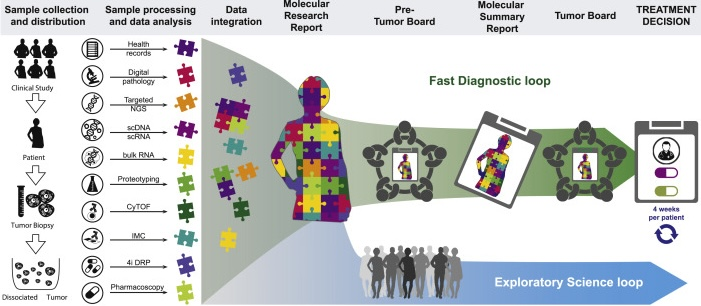
\includegraphics[width=0.95\textwidth]{figures/introduction/tupro.jpg}
  \end{center}
  \caption{Overview of the Tumor Profiler project, adopted from \cite{irmisch2020}. The project is split in two stages: a fast diagonstic loop, which performs multi-modal single-cell profiling on biopsies of incoming cancer patients to supplement traditional diagnostic stragies, and an exploratory science loop, which performs cohort-wide analysis on the collected samples.
  }\label{fig:tupro-overview}
\end{figure}

Over the course of three years, the project applied cutting-edge multi-modal profiling technologies to a total of 240 samples spanning metastatic melanoma, metastatic epithelial ovarian cancer, and acute myeloid leukemia.
These samples are derived from biopsies taken from patients enrolled in one of the participating hospitals.
After the biopsy is taken, it is divided and distributed to one of the technology nodes who profile their split with their respective technology.
The single cell profiling technologies described in the previous section are a subset of the total technologies employed by the study.
Analysis from each node is integrated and distilled into a report and 
this report is further distilled by a "pre-tumor" board and finally by the final tumor board where treatment decisions are made.
For each sample, the target turn around time for collection, profiling, and analysis is two weeks.

\section{Representation learning of scRNA-seq data} \label{sec:scrna-seq}
Raw read outs of single-cell profiling technologies often have statistical properties that are difficult for computational tools to handle.
These statistical properties, present especially in scRNA-seq but applicable for biological data in general,
include challenges like high-dimensionality, heavy-tailed distributions, sparsity, and noisy observations.
Additionally, there are added challenges due to batch effects, 
technical variations that arise from uncontrollable differences in experimental conditions that can result in differences in the measured gene expression levels between different runs, or batches, of the same experiment.
As such, special care must be paid to not only the normalization of data, but their representation as well.
In this section we detail some of the major sources of noise in scRNA-seq data, how they are addressed or not addressed in common normalization strategies, and autoencoder-based approaches to learn compressed and more manageable cellular representations.

\subsection{Normalization and preprocessing of scRNA-seq}
The usual approach to scRNA-seq involves several steps: read extraction, amplification, and mapping.
Read extraction involves converting RNA molecules into complementary DNA (cDNA) and attaching adapters for sequencing.
Then, amplification via PCR generates millions of copies of the cDNA, which are finally sequenced and mapped to a reference genome.
This ultimately generates a (sparse) cell-x-gene count matrix.
To help alleviate biases arising due to variation during the amplification step, unique molecular identifiers (UMIs), a small nucleotide sequence, are concatenated to captured RNA molecules before amplification \cite{islam2014}.
After amplification, the UMIs remove duplicate reads, reduce the impact of PCR biases, and improve the accuracy of gene expression estimates.

A common challenge in the interpretation and analysis of scRNA-seq data is the disentanglement of biological signal from technical noise.
For instance, the source of the sparsity of expressed genes can arise from both a biological limitation on the number of co-expressed genes a cell is able to exhibit and a technical limitation on the rate of capture \cite{breda2021}.
Thus, preprocessing and normalization of scRNA-seq data rely on intuitions of the underlying biological and technical mechanisms.

There are two main sources of variation underlying the measurements made in scRNA-seq,
variation in the capture reads and variation in the relative rate of replication in the amplification step.
Since RNA molecules are distinct entities, their abundances are modeled using discrete probability distributions.
The Poisson distribution is a popular choice to model these variations,
as the number of RNA molecules or UMIs of a given gene in a single cell is typically conceptualized as a count of independent capture events \cite{breda2021},
which is the key assumption underlying the Poisson distribution.
scRNA-seq data can exhibit additional sources of variations, from both technical sources and dynamics in underlying biological mechanisms \cite{hicks2018},
that break these assumptions.
In such cases, a popular choice is the more complex negative binomial distribution \cite{choudhary2022}.
While many methods have been introduced that utilize the negative binomial distribution \cite{lopez2018, risso2018, eraslan2019},
these methods can, in general, be expensive to fit, be difficult to tune, or rely on statistic models that may or may not be correctly modeling the underlying biology \cite{ahlmann-eltze2023}.

The degree to which sparsity in scRNA-seq data arises from biological or technical origins is a controversial issue.
While missing data or zero gene counts can arise from biologically unexpressed genes, they can also arise from technical artifacts,
such as failure to capture reads before amplification.
So called "zero-inflation" or "gene dropout" refers to genes expressed biologically but reported missing due to these technical effects \cite{silverman2020}.
There was convincing evidence for these effects in the early days of scRNA-seq \cite{vallejos2017},
and likelihood-based models were enhanced with mixture terms to zero out counts \cite{pierson2015, dijk2018, lopez2018, huang2018, eraslan2019}.
Recent arguments, however, challenge the prevalence in current scRNA-seq technologies \cite{svensson2020,jiang2022}
and models with zero-inflation terms have shown to perform similarly when they are removed \cite{vieth2017},
yet these arguments still remain controversial or nuanced \cite{cao2021}

The standard normalization of scRNA-seq data is a two step process involving a simple library size normalization followed by a variance-stabilizing log transform \cite{luecken2019}.
While this normalization does not directly address the variation and mechanisms described above, it has been shown to perform suprisingly well \cite{ahlmann-eltze2023}.
The library size normalization addresses a ubiquitous source of confounding in scRNA-seq data.
Observations are reported in the form of gene counts and the total number of these counts from an individual cell is known as its library size.
The library size is determined due to several underlying technical variations including but not limited to capture rate \cite{lytal2020} and influences the magnitude of gene counts.
Therefore, the library size is typically normalized such that the total number of counts within an individual cell is some constant.
After library size normalization, a variance-stabilizing log transform is applied.
Since many gene counts are still zero, a constant offset or pseudocount is applied, $log(x + 1)$ also referred to as \textit{log1p}, to avoid \textit{nan}s.
There is a relationship between the normalized library size and the pseudocount, as smaller library sizes imply, in effect, larger pseudocounts.
This in turn affects the statistics and behavior of lowly expressed genes \cite{ahlmann-eltze2023}.

Even after normalization, the sparsity and high-dimensionality of scRNA-seq data still remain as challenges.
In addition to the filtering genes and cells that exhibit a high degree of sparsity, it is commonplace to select for some subset of highly-variable genes (HVGs).
For example, "house keeping" genes, in charge of basic cellular processes, tend to be constantly expressed at high levels and are relatively uninformative to cellular identity.
Furthermore, there may be a large number of genes that mark for specific pathways, cell types, or other biological processes which may not be present or of interest.
HVG selection aims to remove such genes automatically, by determining non-informative genes whose expression does not change across the population.
Oftentimes, this step can reduce the dimensionality from the tens of thousands to the much more manageable hundreds to thousand \cite{satija2015,zheng2017,stuart2019}.

\subsection{Learning low-dimensional representations with (variational) autoencoders}
Autoencoders (AEs) have emerged has powerful and ubiquitous tools to aid in the modeling and analysis of scRNA-seq data.
These models learn compressed representations of high-dimensional data by training a pair of neural networks, an encoder $\phi$, and a decoder $\psi$,
to map data into and out of a low-dimensional "bottleneck" feature space such that data points can be faithfully reconstructed from their bottleneck representations.
Let $x \in \mathbb{R}^D$ be a data point in the high-dimensional feature space and let its corresponding representation in the low-dimensional space is $z \in \mathbb{R}^d$.
Then $\phi \mapsto \mathbb{R}^D \to \mathbb{R}^d$ \emph{encodes} data points into the bottleneck feature space,
while the decoder $\psi \mapsto \mathbb{R}^d \to \mathbb{R}^D$ \emph{decodes} data points from the bottleneck feature space back into the data space,
that is $z = \phi(x)$ and $x\prime = \psi(z)$ is the resulting reconstructed data point.
The autoencoder is trained, typically with gradient descent methods \cite{kingma2017} to minimize the reconstruction error:
\begin{equation}
  \mathcal{L}_{ae}(\phi, \psi; x) = -\frac{1}{2} || x - x\prime ||^2
\end{equation}

The popular Variational Autoencoders (VAEs)~\citep{kingma2013} take a generative approach and are frequently applied to scRNA-seq data \cite{lopez2018, huang2018, eraslan2019, lotfollahi2019}.
In these models, the bottleneck space is often called a "latent" space due to its probabilistic interpretation.
Here $\phi$ parameterizes the likelihood of the data given the latent representation $p_\phi(x|z)$ and $\psi$ parameterizes the posterior probability of its latent representation $q_\psi(z|x)$.
VAEs jointly learn $\phi$ and $\psi$ to maximize a lower bound to the probability of the data $p(x; \phi, \psi)$, achieved in practice by minimizing
\begin{equation}
    \mathcal{L}_{vae}(\phi, \psi; x) = -\log p_\phi(x | \hat{z}) + \mathcal{D}_{KL}(q_\psi(z|x) || p(z))
    \label{eq:vae-loss}
\end{equation}
where $\hat{z} \sim q_\psi(z|x)$, $\mathcal{D}_{KL}$ is the Kullback-Leibler (KL) divergence,
and $p(z)$ is a prior distribution over latent representations.
$p(z)$ and $q_\psi(z|x)$ are typically restricted to Gaussians since the resulting KL divergence has a closed-form solution.
The KL term in equation \ref{eq:vae-loss} is often regarded as a regularization term that enforces the "compact-ness" of the latent space.
When applied to scRNA-seq data, it is common to use a hyperparameter $\beta$ that tunes the strength of the regularization, 
$-\log p_\phi(x | \hat{z}) + \beta \mathcal{D}_{KL}(q_\psi(z|x) || p(z))$,
and is related to the variance of the prior distribution $p(z)$.

\section{Learning to align cellular states across contexts}
We have seen that in order to understand complex biological processes, such as the mechanisms governing the development of cancer, cellular behavior must be understood across many time points and levels, e.g. from its mutational state, levels of gene regulation, abundance of signaling proteins, etc.
Although technologies exist to measure cells on each of these levels,
a common shared limitation is their requirement to consume or destroy profiled cells.
So while we would ideally like to make multiple observations of an individual cell, for example with different profiling technologies or at different points in time, we are typically limited to make only one observation.

A major focus of this thesis is the development and applications of methods that can \emph{reconstruct} multiple observations of individual cells with computational approaches.

In this case, the general strategy is to take some cellular sample
and observe it in the desired multiple states
by dividing the sample in such a way that the set of cells within each observation are similar in composition.
The challenge of the methods development is to reconstruct the corresponding cellular states by \emph{alignment} of these multiple observations.
Say $\eta$ represents the distribution of cellular states representing the sample of interest, and $\mu$ and $\nu$ represent the distribution of cellular states in our contexts of interest (for simplicity we assume there are only two contexts).
We assume that $\mu$ and $\nu$ are somehow derived from $\eta$ and our aim is to then describe how to align $\mu$ and $\nu$.
This alignment appears in two main paradigms, described below:

\begin{figure}[htp]
  \begin{center}
    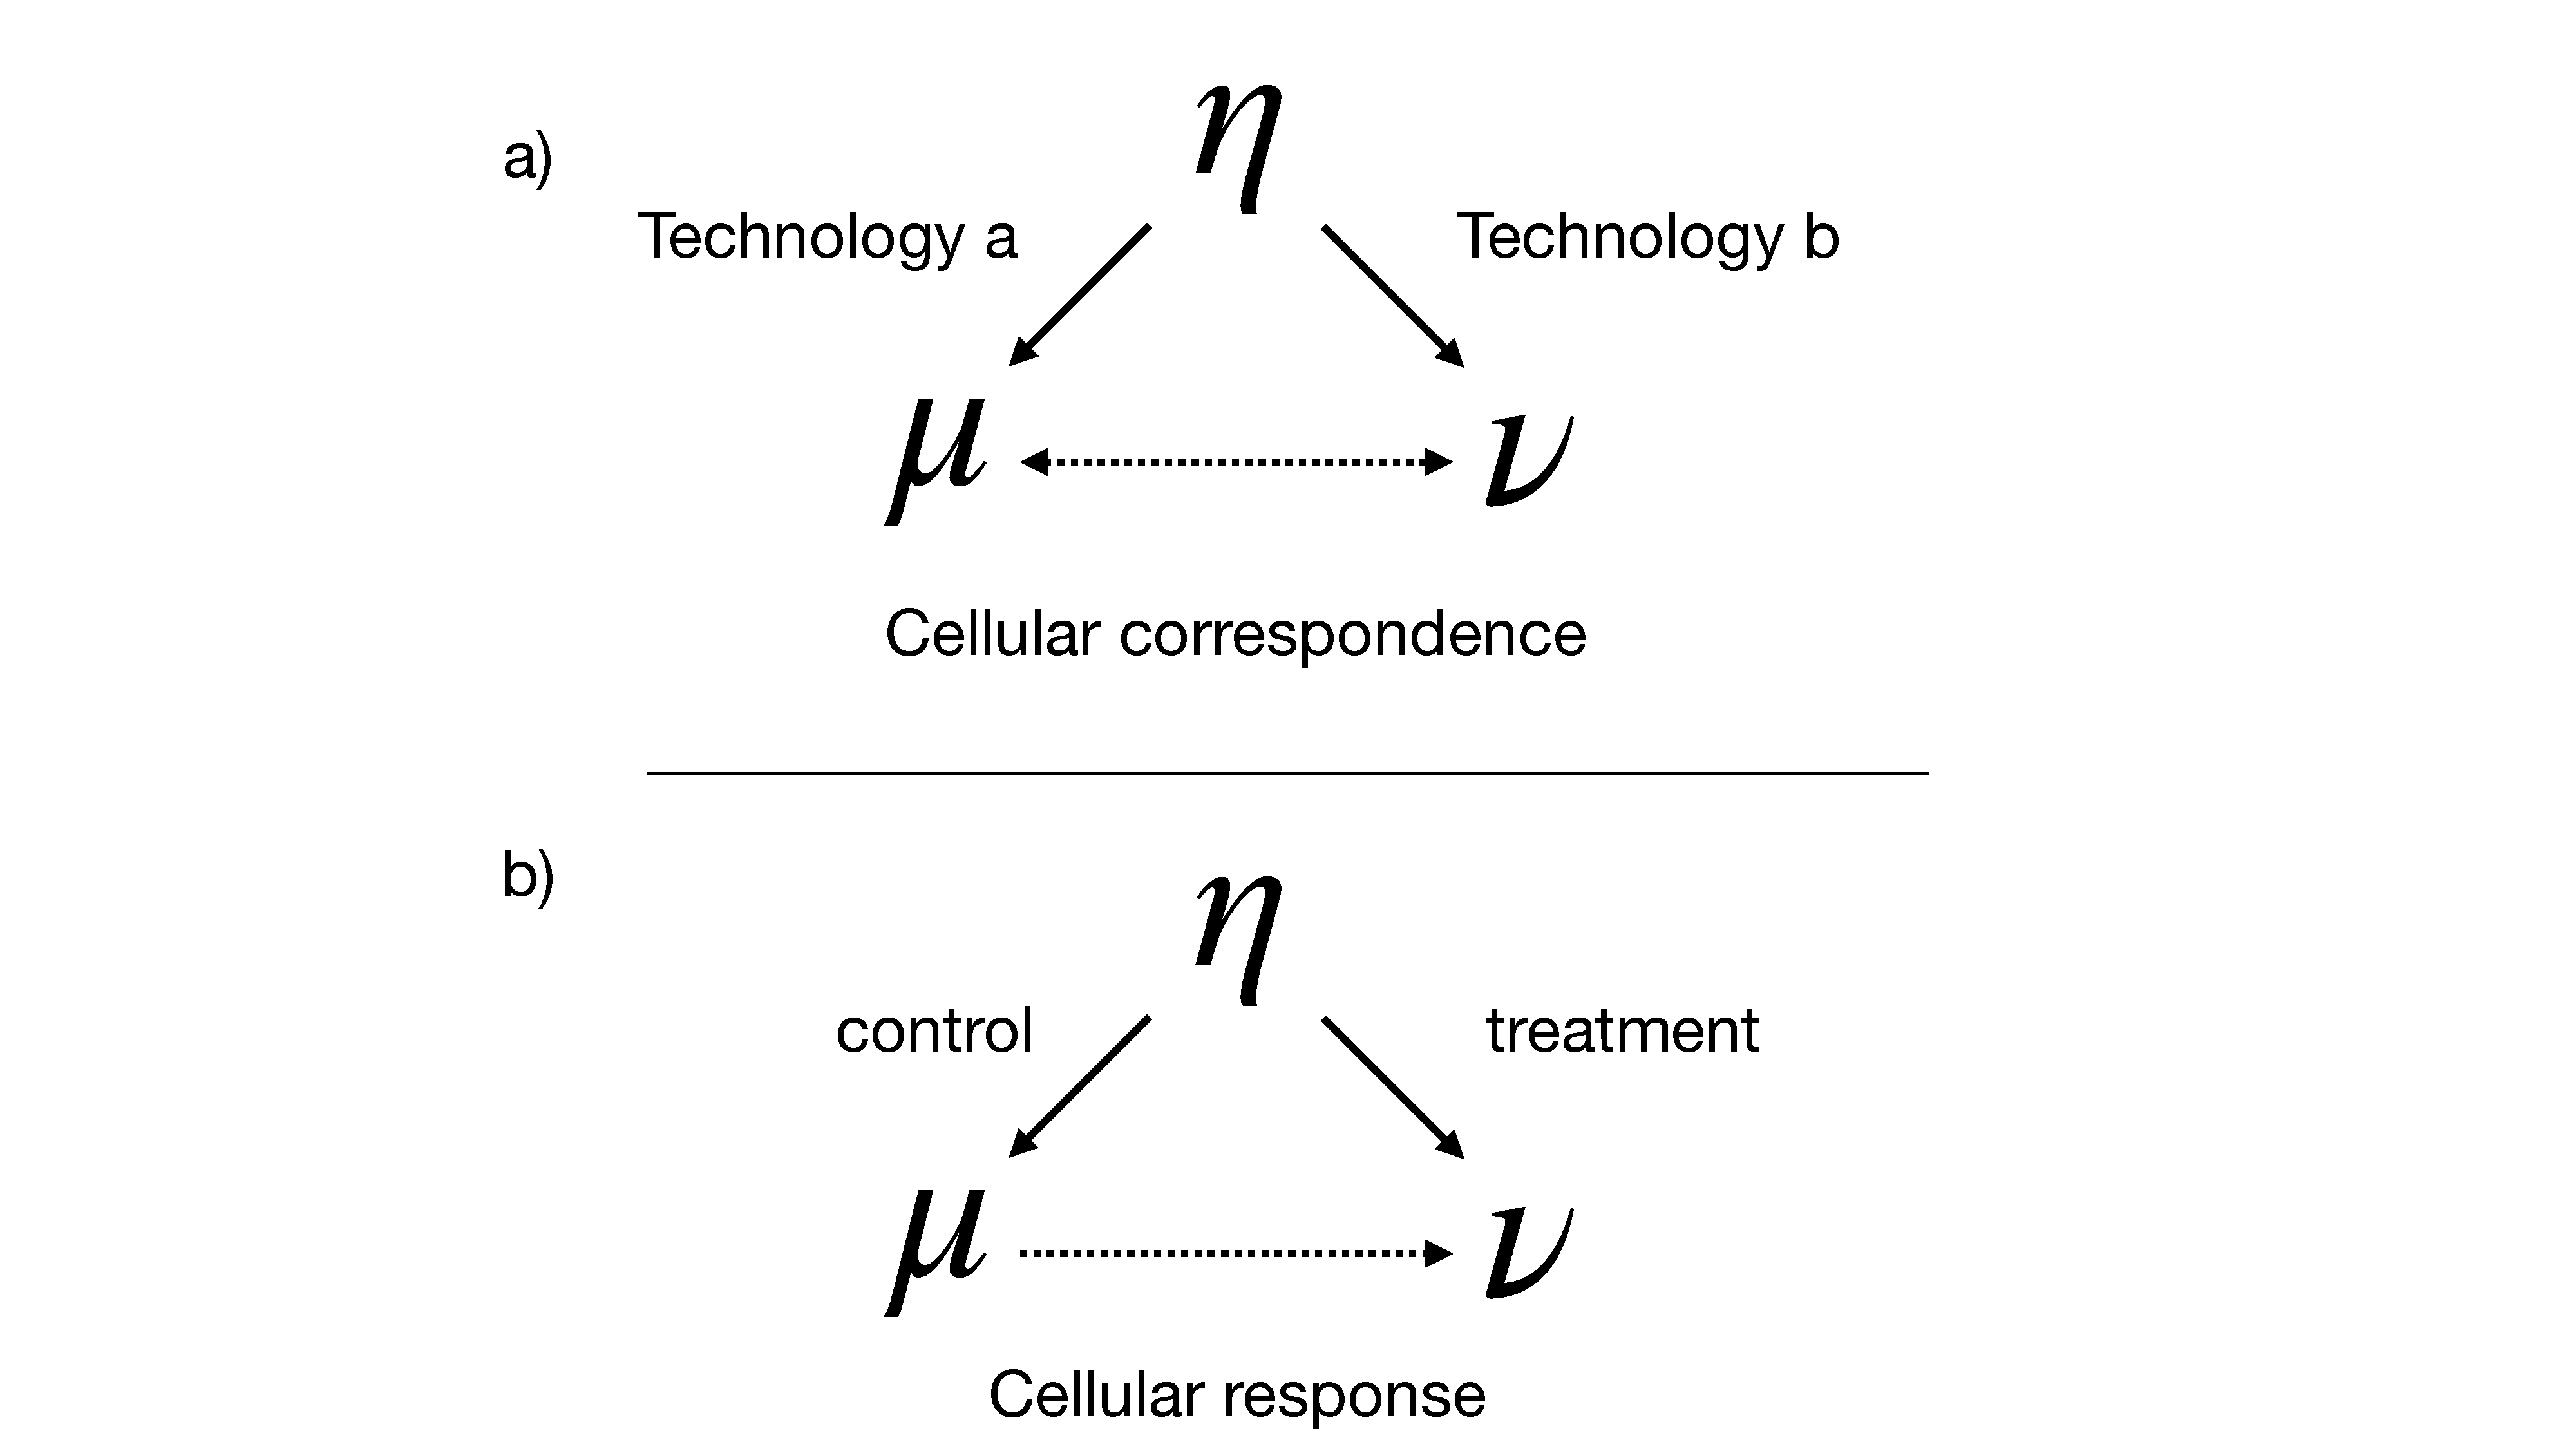
\includegraphics[width=0.95\textwidth]{figures/introduction/thesis-overview-pgm.pdf}
  \end{center}
  \caption{Learning to align single-cell populations. $\nu$ represents some holistic distribution of cellular states that is manipulated or projected into observable distributions $\mu$ and $\nu$.
  In this thesis, methods are developed to align $\mu$ and $\nu$ in order to recover or understand some biological process or state.
  \textbf{a)} multi-modal integration. $\mu$ and $\nu$ are realized through different single-cell profiling technologies. \textsc{SCIM} \cite{stark2020} is developed to construct multi-modal single-cell observations.
    \textbf{b)} single-cell perturbation responses. $\mu$ and $\nu$ are represent the control and perturbed population states. \textsc{CellOT} \cite{bunne2023} is developed to recover the perturbation responses of individual cells.
  }\label{fig:thesis-overview-pgm}
\end{figure}

\paragraph{Constructing holistic view of cells}
Often it is advantageous to understand cellular state in the context of multiple modalities,
for instance, to understand the joint-wise state of gene expression and protein levels.
Here, $\mu$ and $\nu$ can be considered projects of $\eta$ from some abstract space representing a holistic cellular state into their respective observable domains, e.g. gene expression space or protein space, as summarized in Figure \ref{fig:thesis-overview-pgm}a.
The key complication here is that $\mu$ and $\nu$ are typically in distinct feature spaces that might not have a trivial correspondence.
For instance, the relationship between genes and proteins are known to not be 1-to-1 \cite{edfors2016}.
Chapter \ref{ch:scim} describes SCIM, a framework that performs multi-modal single-cell integration in the absence of corresponding cellular feature sets.

\paragraph{Constructing time-resolved cellular observations}
The cellular responses to perturbations can be considered as a temporal process.
Cells are exposed to some agent of perturbation, such as a drug treatment, that causes a cascade of signal activation within the cell, changing its state.
Here, $\mu$ and $\nu$ can be considered observations of $\eta$ within the same observational domain but under different conditions, summarized in Figure \ref{fig:thesis-overview-pgm}b
Typically $\mu$ will refer to the population treated and profiled with some control condition, while $\nu$ will refer to the population treated with the perturbation of interest and profiled after some time has passed.
The key complication here is that the underlying cellular populations will be heterogeneous in composition and response, and these complicated responses will need to be recovered without access to paired input-output cellular states.
Chapter \ref{ch:cellot} describes CellOT, a framework to learn and predict such heterogenous perturbation responses from uncoupled cellular observations using recent advances in neural optimal transport.
Chapter \ref{ch:cohort} explores the clinical utility of such an approach by applying it to learn and predict the responses of a cohort of melanoma patients to a set of standard-of-care treatments.

\chapter{Learning to align single-cell multi-modal profiles}

\section{Background}
The ability to dissect a tissue into its cellular components to study them individually or to investigate the interplay between the different cell type fractions is an exciting new possibility in biological research.
These lines of research have yielded important insights into the dynamics of various diseases, especially for cancer \cite{chevrier2017,tirosh2016}.
Recent advances in single-cell technologies enable molecular profiling of samples with greater granularity at the transcriptomic, proteomic, genomic as well as the functional assays level \cite{irmisch2021,rozenblatt-rosen2017}.
While each of these data modalities offer insight into different types and levels of internal cellular processes,
a \textit{holistic} understanding of cellular state could be obtained through the combination or integration of these modalities.
Knowing the measurement of multiple modalities for individual cells would deepen our understanding of the cellular mechanisms at play in, for instance, the tissue microenvironment, and construct a comprehensive molecular view of profiled samples.

A key challenge towards such integration, however, lies in the limitations of profiling technologies.
Since ubiquitous technologies, such as scRNA-seq and CyTOF, consume the profiled cells, it is typically not possible to observe these cells in more than one modality.
While technologies capable of measuring multiple modalities simultaneously are emerging \cite{stoeckius2017,zhu2020}, they remain limited in terms of scalability and practicality.
Thus, the multi-modal integration of cellular processes falls to computational methods.
Given observation datasets across individual profiling modalities, these methods typically assume that the samples profiled in each modality are somehow similar in composition, and perform integration bo constructing and \textit{alignment} across these datasets.
A critical complication towards this alignment lies in the weak correspondences between the feature sets over these modalities
For instance, there does not exist a one-to-one correspondence between genes (as profiled by scRNA-seq) and proteins (as profiled by CyTOF).
Thus, proper alignment is a challenging task.

%\bold{Related work}
While multiple data integration tools have been developed, most approaches either depend on or impose feature correspondences \cite{stuart2019,welch2019}, or are designed to applied to a limited set of modalities, for instance, scRNA and scDNA data \cite{campbell2019,mccarthy2020}.
To the best of our knowledge only two other approaches have been published \cite{amodio2018,welch2017} able to perform integration over general modalities.
MAGAN \cite{amodio2018} is a Generative Adversarial Network capable of aligning the manifold between two technologies that relies on a feature correspondence loss.
MATCHER \cite{welch2017} is based on a Gaussian process latent variable model (GPLVM) \cite{lawrence2004} that can integrate technologies if their underlying latent structures can be represented in one dimension, applicable, for example, to model monotonic temporal processes.
ather yet unpublished methods, such as MMD-MA \cite{liu2019} and UnionCom \cite{cao2020}, rely on large kernel matrices which limit their scalability when using datasets of the sizes generally produced by molecular profiling.

Here, we propose Single-cell Integration via Matching (SCIM), a method to match cells across different single-cell ’omics technologies.
Our approach is universal, in the sense that it is in principle applicable to any single-cell technology and overcomes the scaling issues of contemporary approaches.
Further, we do not assume the existence of paired features between two technologies.
This allows for the integration of technologies that measure for example the expression of a disjoint set of genes, or the integration of gene expression with image features as long as the underlying latent structure is present in those features.

%\graphicspath{{figures/integration}}

\section{Single-cell integration via Matching}
SCIM performs multi-modal single-cell integration in two steps.
First, we construct an integrated latent space using an adversarial autoencoder framework \cite{Makhzani2015} wherein representations are invariant to their corresponding technologies,
inspired by a model proposed previously \cite{Uhler2019} and further extended in ~\cite{Yang2019}
In the second step, we perform a strong pairwise alignment of datasets from each modality via a cell-to-cell matching strategy that efficiently extracts cross-technology cell matches from the latent space.
SCIM assumes a shared latent representation between technologies but, unlike other approaches, does not require one-to-one or overlapping correspondences between feature sets.
SCIM scales well in the number of cells in the input through the use of neural-nets, end-to-end training and an efficient bipartite matching algorithm.
Finally, this training scheme allows for the addition of an arbitrary number of technologies, which can be trained in parallel.

\begin{figure*}[ht]
    \centering
    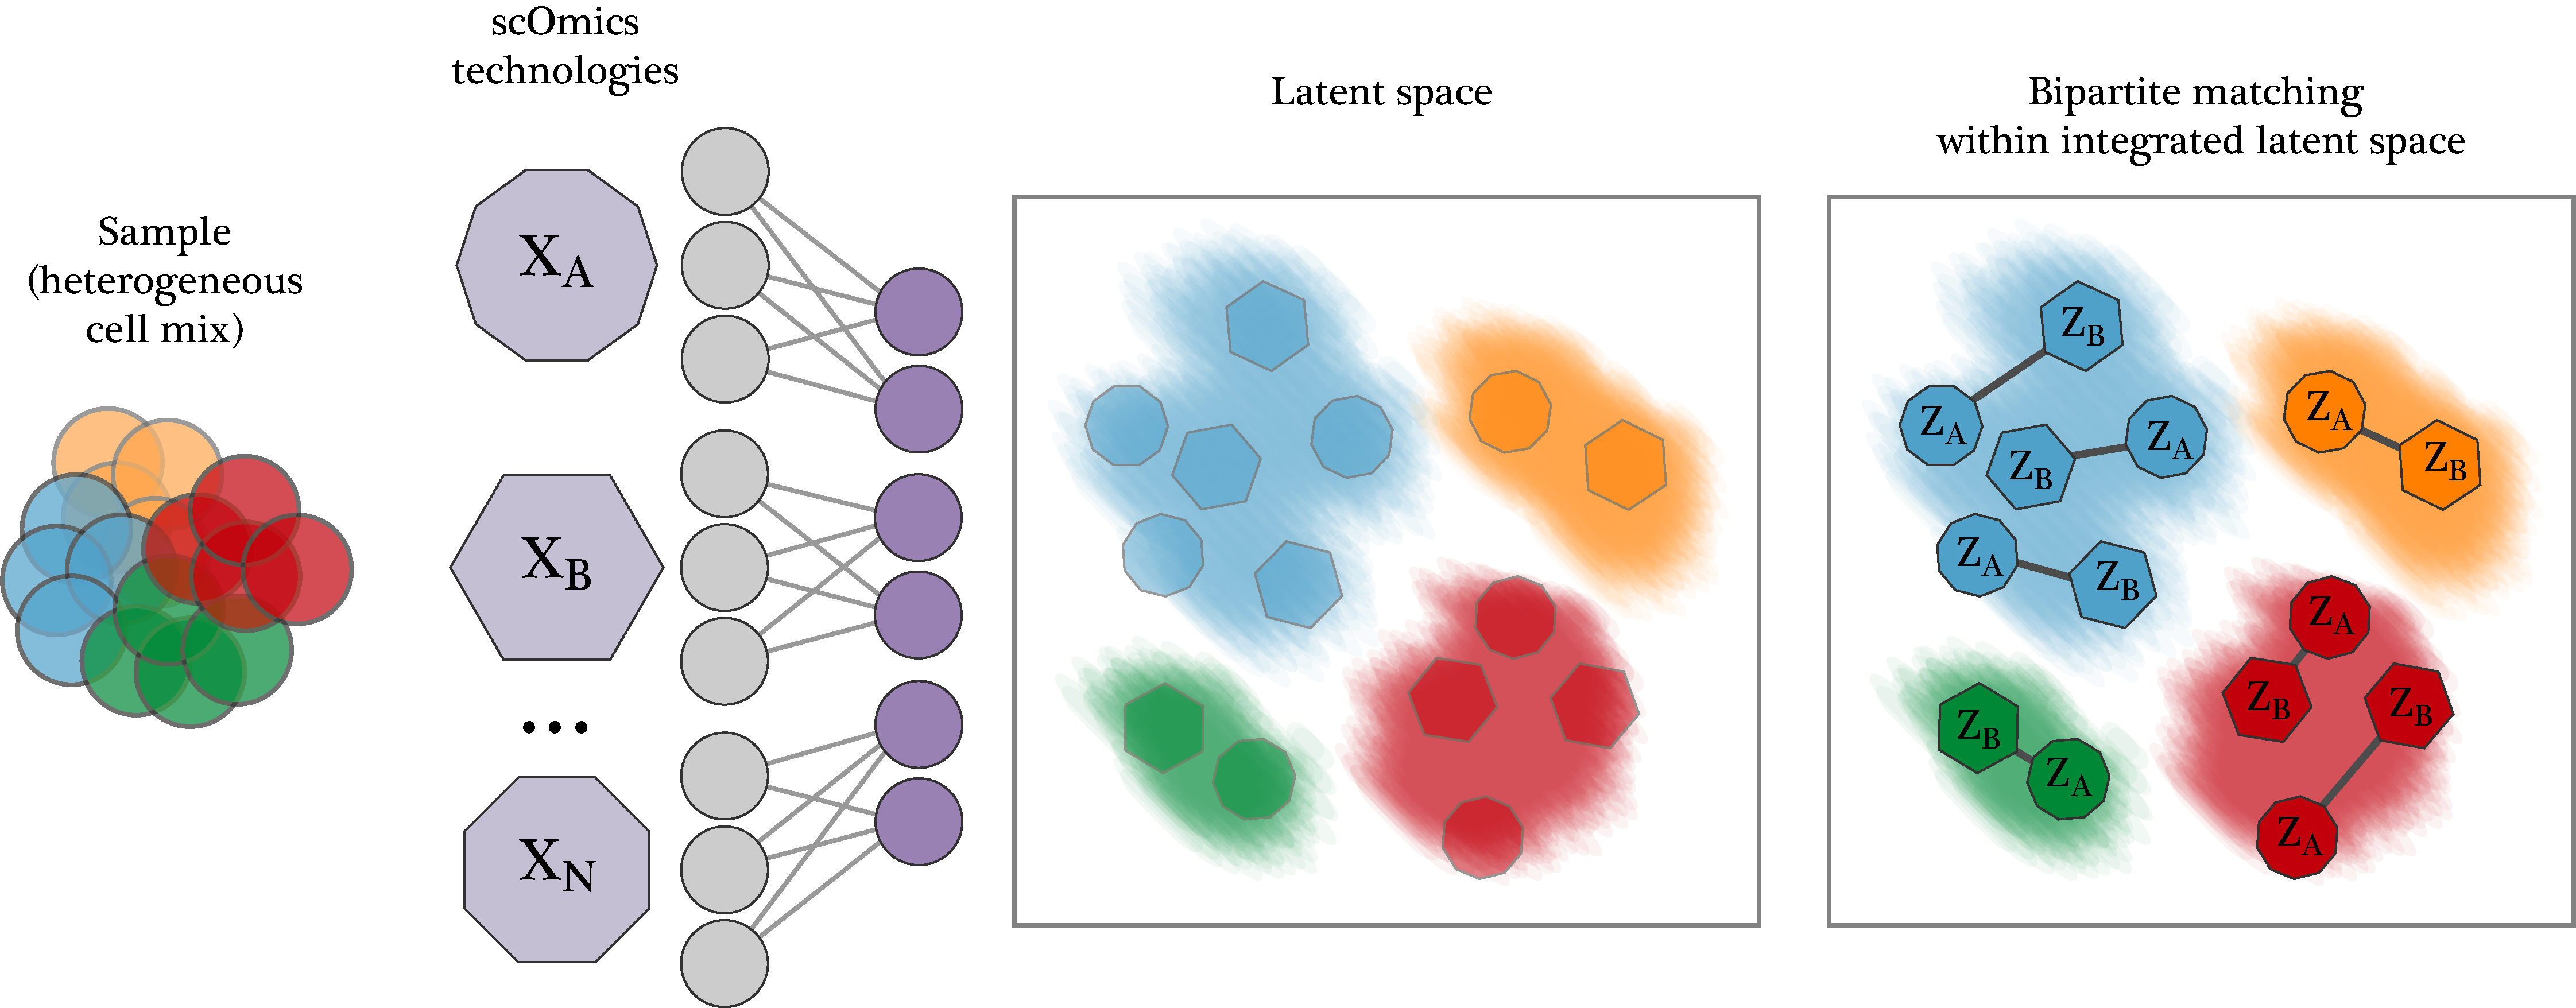
\includegraphics[width=\textwidth]{figures/integration/pipeline.png}
    \caption{
    SCIM performs a pairwise matching of cell across multiple single-cell 'omics technologies. We assume that the input of each technology comes from the same (or similar) heterogeneous cell mix, depicted on the left. Technologies generate a set of single cell 'omics datasets (violet polygons) in parallel (e.g. $X_A$, $X_B$, $X_N$).
    These datasets are represented as matrices of cells-by-features, where features are specific to the profiling technology, but could be gene expression, protein levels, etc.
    SCIM proceeds to map cells into a technology-invariant latent space (left box) using an autoencoder framework and an adversarial term to keep technologies well integrated.
    Here the latent representations capture the underlying structure in the cell mix (colored clouds) and analogous cells from different technologies (colored polygons) are placed in proximity.
    To integrate datasets, a fast bipartite matching scheme is applied, matching cells pairwise among datasets to cross-technology analogs, using their latent representations (right box).
    }
\end{figure*}

\subsection{Constructing technology-invariant representations}
SCIM encodes datasets into a shared latent space that is constructed to have two properties:
1) the inputs should be able to be reconstructed from their latent representations, as is typically achieved by vanilla VAEs \ref{sec:autoencoders}
and 2) the latent representations of each technology should be well-integrated such that they are indistinguishable from each other.
In a successful integration the resulting latent space will have corresponding cells across all technologies represented in close proximity.

To construct an integrated latent space, SCIM uses a modified adversarial auto encoder framework.
This consists of the following networks: a pair of encoder ($\phi_k$) and decoder ($\psi_k$) networks for each technology $k$ and a single discriminator network ($\gamma$) acting on the latent space.
This discriminator is a binary classifier trained to identify the latent representation of some source technology from latent representations of all other technologies using a binary cross entropy loss.

SCIM yields an integrated latent space by minimizing the reconstruction error while adversarially fooling the discriminator.
Given the measurements of a batch of cells from the target modality $t$, $x_t$, and the (fixed) latent representations of a batch of cells from the source modality $s$, $\hat{z}_s \sim \phi_s(x_s)$,
% TODO: major: fix SCIM equations, write as min-max
\begin{equation}
	a = b
  \label{eq:scim-loss}
\end{equation}

$\mathcal{L}_{nll}$ is the negative log-likelihood of the inputs under their reconstruction.
$\mathcal{L}_{adv}$ is the discriminator’s classification error when trying to classify the latent representation samples $\hat{z}_s$ or $\hat{z}_t$ as the source or target technology.
$\beta$ is a hyperparameter weighing the influence of the adversarial loss.
%At the same time, c is trained to correctly classify the technology of the z^s and z^t samples.

\paragraph{Latent space orientation}
Correctly orienting the latent space in an unsupervised manner is a challenging task \cite{Locatello2019,Uhler2019}.
Consider, for example, a simple monotonic temporal process.
The latent representations for one dataset could be oriented from start to end, while another could be oriented from finish to start \cite{Welch2017}.
Equation \ref{eq:scim-loss} satisfied, the representations are well integrated and inputs can be correctly reconstructed from them, yet the inter-dataset relationships are misaligned.
\citet{Makhzani2015} address a similar problem by concatenating one-hot representations of labels reflecting intra-technology structure (e.g. cell type is an appropriate choice for ’omics datasets) to the discriminator inputs, showing that this supervision is necessary to orient the latent space.
Furthermore, \citet{Locatello2019} argued that only a small number of labels are actually needed to achieve orientation.
To this end, we adopt a semi-supervised approach for some experiments by adding a ‘censored’ label and randomly relabel cells in the training set.

\paragraph{Model architecture}
Unless specified otherwise, we adopt the following architecture settings.
All networks use the ReLU activation \cite{agarap2018}.
We set the latent dimension of all models to eight, but observed this choice to be flexible.
We use discriminator networks with two layers and eight hidden units each.
The Spectral Normalization framework \cite{Miyato2018} is used during training, which has been argued to stabilize discriminator training by effectively bounding its gradients.
We use a Gaussian activation for all decoders, a 2 layer architecture with 64 hidden units for all simulated data networks, a 2 layer architecture with 8 hidden units for all CyTOF networks and a 2 layer architecture with 64 hidden units for all scRNA networks.
The number of features and complexity of data is considered when choosing capacity and depth.

\paragraph{Optimization}
Optimization proceeds by iteratively fixing one technology as the source and one technology as the target.
In the case of more than two technologies, the technology corresponding to the discriminator’s positive class must either be the source or target technology.
Optimization proceeds with an inner and outer loop.
In a single inner loop step, the latent representations of the source technology are fixed and Equation \ref{eq:scim-loss} minimized with gradient updates to the encoder and decoder of the target modality $t$ using gradients computed on the batch $x_t$.
This process is repeated multiple times and then one step of the outer loop is performed.
In a single outer loop step, the discriminator is updated to classify $z_s$ and $z_t$.
All networks are optimized using the ADAM algorithm \cite{Kingma2013}.


\paragraph{Model Selection}
Due to the min–max nature of adversarial training, model comparison is challenging since one cannot directly compare the minimized objective functions of converged models \cite{Lucic2017}.
While the computer vision community has introduced a number of metrics specific to the image domain to help compare models \cite{Heusel2017,Salimans2016}, here we need to validate the quality of a set of lower-dimensional latent representations.
To achieve this, we utilize a k-Nearest Neighbor (kNN)-based divergence estimator \cite{Wang2009}.
The divergence score between two sets of codes $Z_s$ and $Z_t$ is calculated as:
% TODO: minor: typeset eqn
\begin{equation}
	a = b
\end{equation}
This estimator approximates a symmetric variant of a KL divergence, a measure of how much two distributions differ, using only empirical data.
The divergence estimate is computed between the latent representations of the source technology and the target technology to measure the alignment of codes from the two technologies.
Model selection can proceed at scale by selecting parameter configurations that align technology distributions and have low reconstruction error.

\subsection{Bipartite matching of single-cell embeddings}
In its second step, SCIM performs multi-modal integration by identifying pairs of corresponding cells across two modalities using their representations in the latent space constructed in the first step.
We identify pairs by solving a combinatorial bipartite matching problem \cite{Ahuja1993,DellAmico2000}, wherein the bipartite graph is constructed by connecting cells between each pair of technologies, weighted by their distances in the latent space.
The bipartite matching problem then identifies an optimal set of paired cells that minimizes the total edge cost of all matches.
In order to achieve this efficiently and at scale, we approximate the full bipartite graph with a k-Nearest Neighbors (kNN) graph that identifies a set of potential matches for each cell and reduces the complexity of the problem.
We then extend the graph to account for single-cell data characteristics and solve the bipartite matching within a general framework of Minimum-Cost Maximum-Flow problems \cite{Ahuja1993,Klein1967}.

\paragraph{Min\-cost Max\-flow matching}
Based on a Euclidean cost matrix, we aim at finding the maximum number of cell pairs with minimum cost.
This corresponds to finding a maximum flow that can be pushed through the graph, where each edge between cells has capacity 1, while minimizing the overall cost.
To solve the Minimum-Cost Maximum-Flow problem in a computationally efficient way we use an implementation of the network simplex algorithm \cite{Kiraly2012}.

\paragraph{Evaluation}
Since it is not possible to profile the same cell in multiple modalities, we lack a set of ground truth cell pairs to evaluate against.
The integration quality is instead evaluated on several levels, specific to the samples and modalities integrated.
First, when cell type labels are present, the accuracy corresponding to the fraction of true positives with regard to cell-type label is reported.
Cell types can be determined in a technology-specific manner and the accuracy is reported on a common denominator.
If more fine-grained cellular information is available, such as pseudotime, a direct comparison of this quantity is carried out.
Furthermore, in real-world data settings we utilize the raw marker expression to investigate correspondence of the matched cells.
Namely, Spearman’s and Pearson’s correlation coefficients are computed between the expression values across matches.

\subsubsection{Graph modifications}

\paragraph{kNN subgraph approximation}
Given the large number of cells in single-cell datasets, we reduce the search space to the $k$ most likely potential matches.
For each pairwise integration task, two kNN graphs are built: the first uses the source data queried by the target technology cells, and the second uses target data queried by the source technology
That is, each cell in the source technology is connected to its $k$ nearest neighbor cells in the target technology and each cell in the target technology is connected to its $k$ nearest neighbor cells in the source technology.
The union of this graph is then used in the bipartite matching solver.
The sparsity of these connections, regulated by the choice of the hyperparameter $k$, corresponds to a trade-off between the computational performance (memory usage, run time) and the final matching accuracy.

\paragraph{Null Cell}
The bipartite matching, Figure \ref{fig:null-cell} makes the assumption that each cell has a singular corresponding sibling in its paired technology.
However, it is reasonable to expect that differences between profiled samples exist that would invalidate this assumption.
To allow for mismatches due to this expected variation in cellular composition,
we expand the kNN graph with sparse connections by adding a densely connected \textit{null cell} with high capacity and relatively large edge weight. 
This allows to capture potentially poorly matched cells by keeping them unassigned.
The magnitude of the null match penalty is a hyperparameter that corresponds to a given percentile $p$ of the overall costs.

\begin{figure}
  \begin{center}
    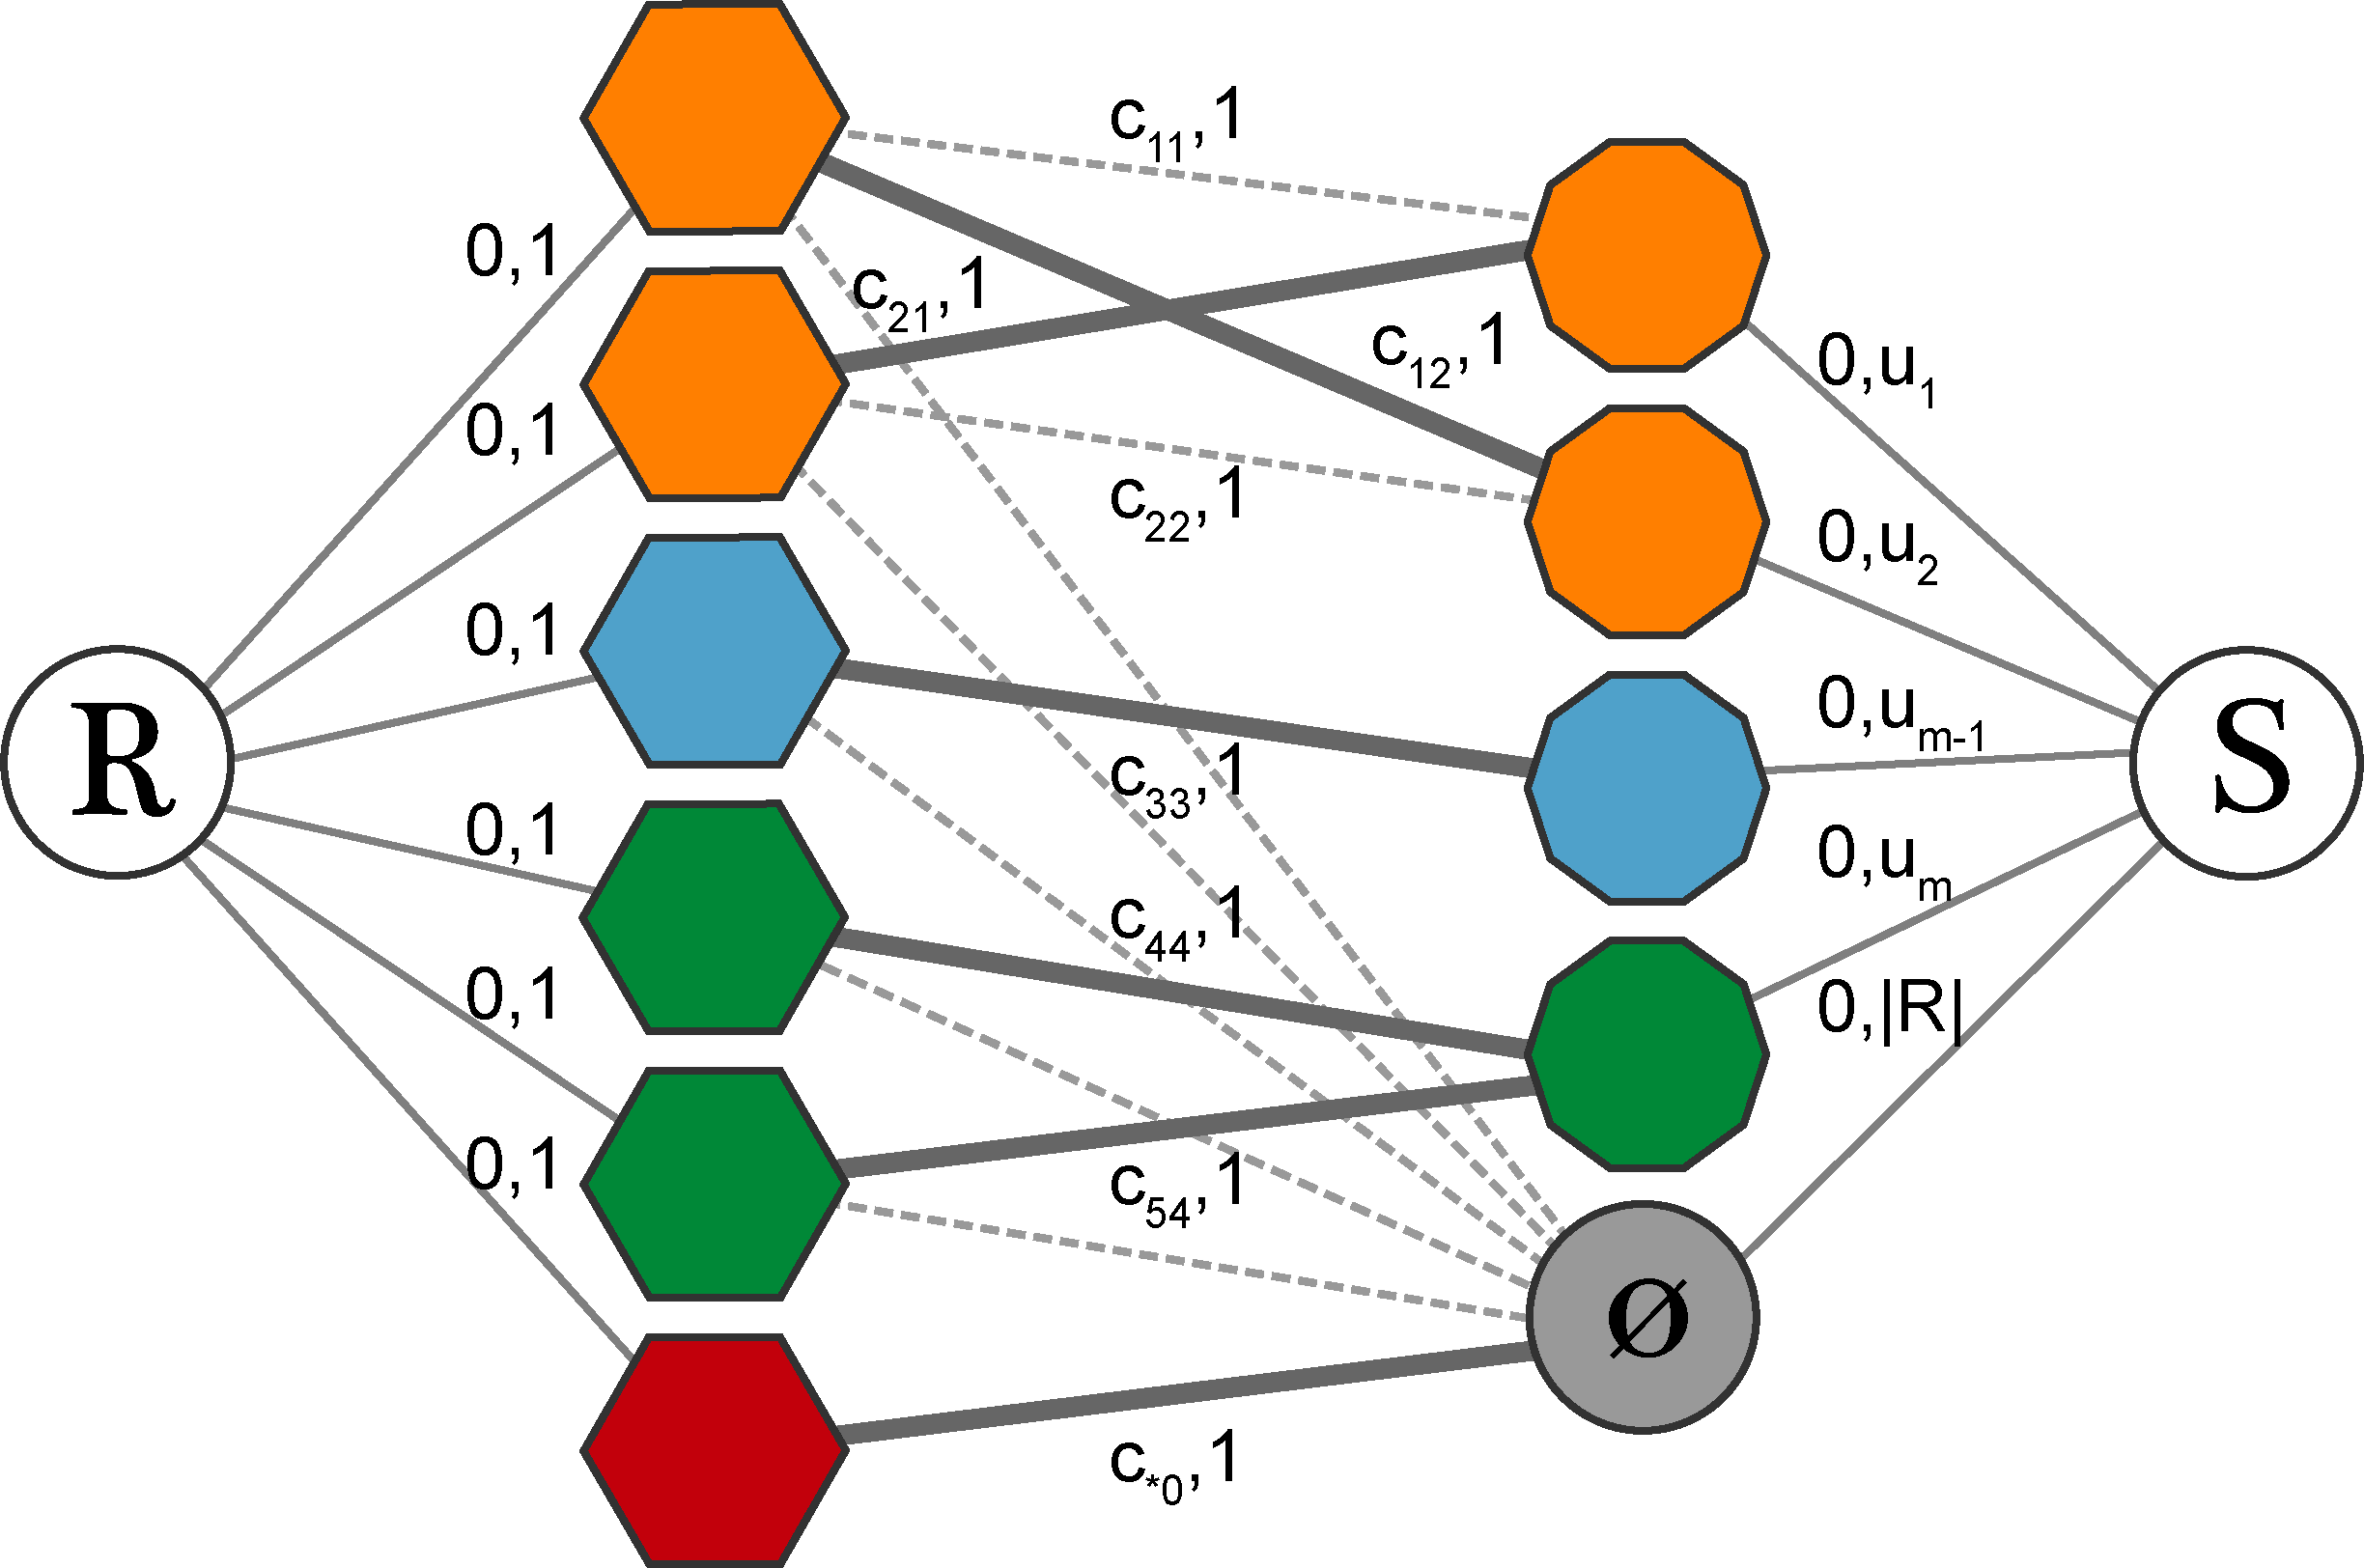
\includegraphics[width=0.95\textwidth]{figures/integration/null-cell.png}
  \end{center}
  \caption{Fast bipartite matching using a customized Minimum-Cost Maximum-Flow framework. Nodes correspond to cells with technology represented by shape, i.e. hexagons and decagons. R and S represent root and sink nodes. Edges correspond to the sparse connections between the cells, resulting from a kNN search. Edge labels indicate matching cost (first value) and edge capacity (second value). Many-to-one matches in unbalanced datasets are enabled by increasing the capacities ui (for i $\in$ 1;  . . ; m). The null node, colored in gray, captures matches of cells (from the bigger dataset on the left-hand side of the graph) that lack a close enough analog in the other technology. Its capacity equals the cardinality of the bigger dataset and the null match penalty is relatively high. The thicker lines linking the nodes represent the actual matches selected by the algorithm.}
  \label{fig:null-cell}
\end{figure}

The extended graph structure is depicted in Figure XX, where $R$ and $S$ refer to the root and sink nodes, respectively.
Furthermore, to account for differences in the number of cells between modalities ($n$, $m$), we allow for one-to-many matches by increasing the capacity of the edges incoming to the sink ($u_i$ for $i \in {1, \ldots, m}$, assuming the nodes linked to the sink correspond to the smaller dataset, i.e. $m \leq n$.
To prevent all matches from collapsing onto a very small set of nodes, we constrain the incoming sink capacities, excluding the null node, to equal the cardinality of the bigger dataset divided by the cardinality of the smaller dataset, with the capacities distributed uniformly across the sink edges.
If more than two data modalities are present, the bipartite matching is solved sequentially by obtaining pairwise matches between technologies.

\section{Multi-modal integration of simulated data}
Since we are unable to observe the same cell in more than one modality, simulated data is crucial for understanding and benchmarking integration methods.
Simulated data allows us to generate controlled datasets with known ground truth, allowing us to assess the performance of these integration methods and identify their strengths and limitations.
Here we mimic the properties of multi-modal single-cell datasets and compare our approach with currently available methods.

\subsection{Simulating multi-modal single-cell datasets}
 We generate three single-cell 'omics-styled technologies that share a common latent structure without direct feature correspondences using the single-cell simulation tool PROSSTT \citep{papadopoulos2019}.
Given a tree that represents some underlying branching cellular developmental process, PROSSTT parameterizes a negative binomial distribution to generate observations of cells along this trajectory.
In order to obtain three datasets that share a common latent structure yet lack any correspondences between features,  we use the same tree input but run PROSSTT under different seeds.
We utilize a five branch tree with different branch lengths (Figure \ref{fig:prosstt5-pseudotime-inverted}),
and generate high-dimensional datasets consisting of 64,000 cells with 256 markers.

\begin{figure*}[htp]
    \centering
    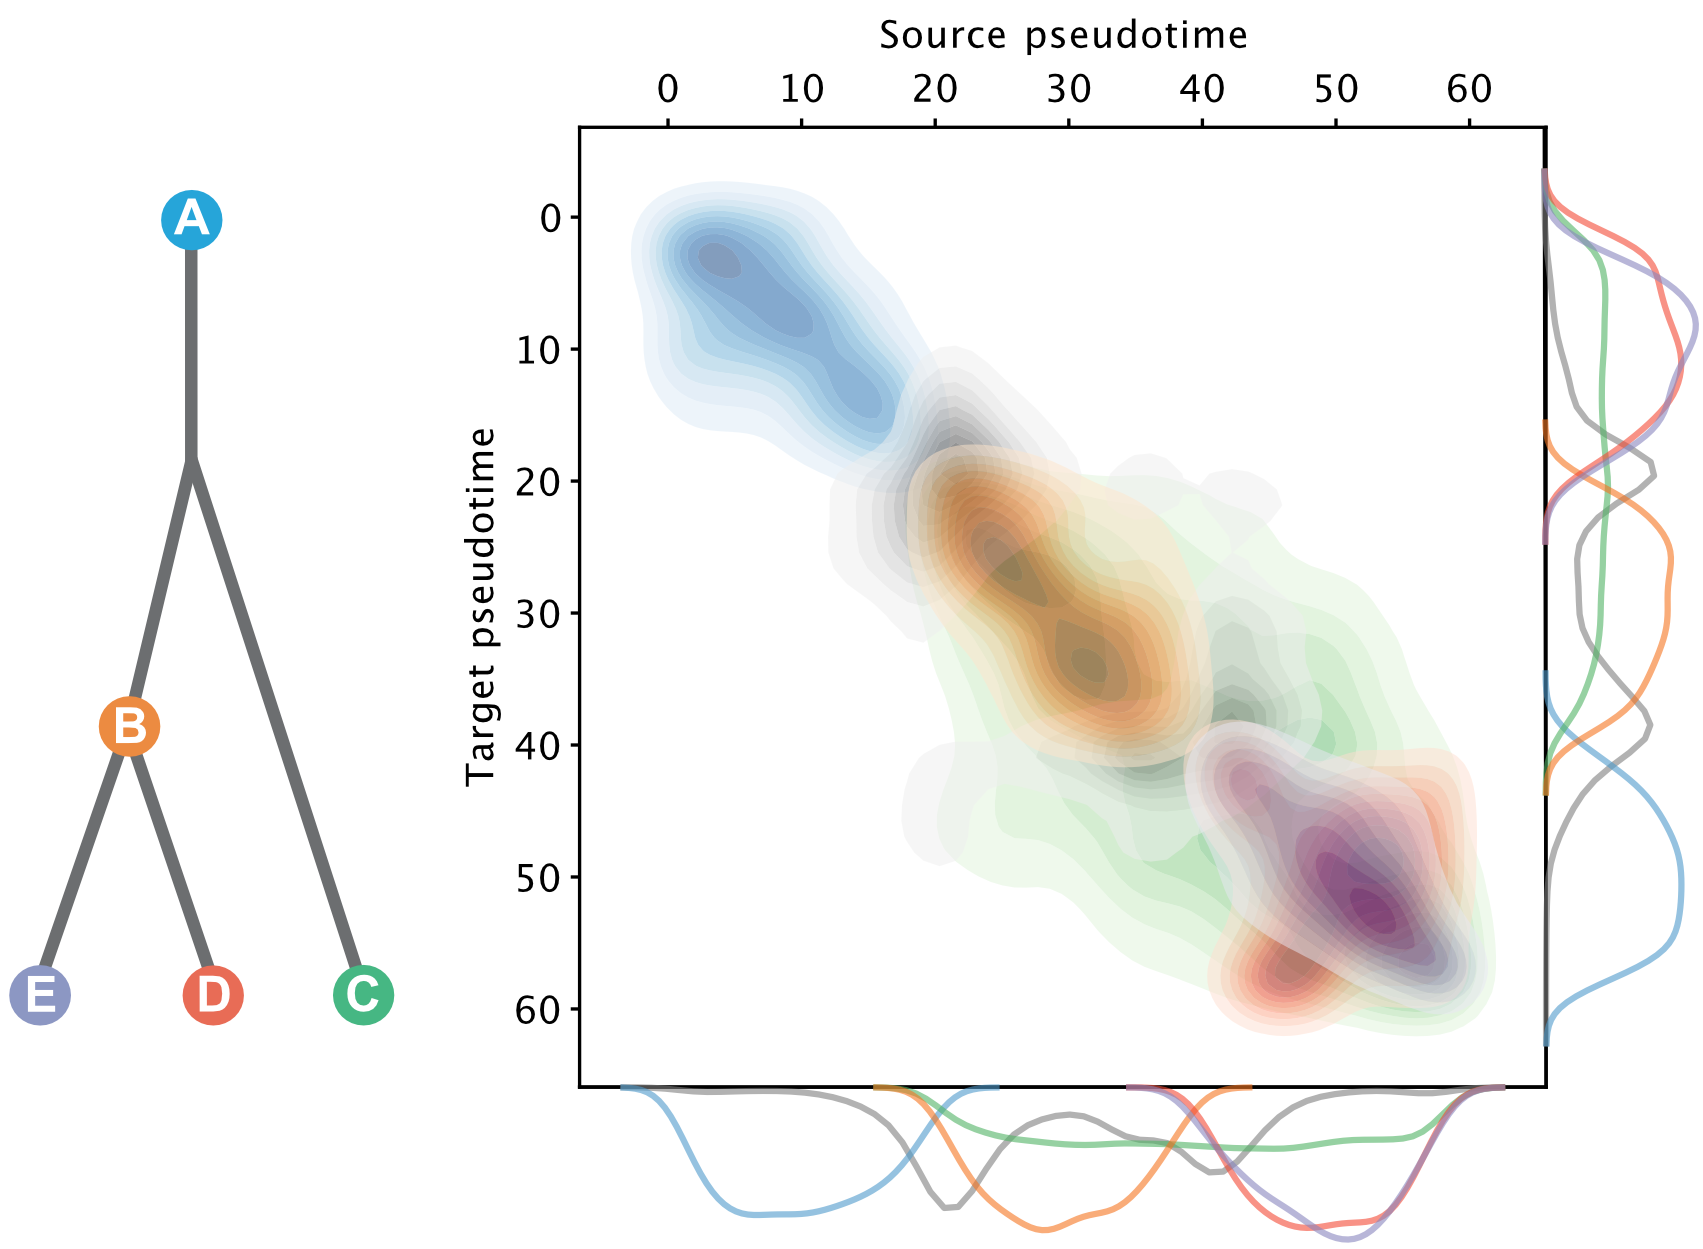
\includegraphics[width=\textwidth]{figures/integration/pseudotime-kde-tree-inverted_thick.png}
    \caption{
    Evaluation of cross-technology cell matches made by SCIM on the simulated data. The tree defining the temporal branching process underlying the simulated data is shown on the left. Cells are matched across datasets pairwise using the bipartite matching scheme and the results are depicted on the right hand-side. The Results are shown as a density plot of pseudotime values across matched cells between the source technology (x-axis) and the target technology (y-axis). Cells matched to the same branch label are colored according to the branch-color scheme (accuracy: 86\%), while mismatches are depicted in grey and appear mostly in the branching points. Marginal distributions of cell pseudotime for each branch are shown at the bottom (source technology) and left (target technology) of the density plot. We report a correlation of 0.83 (Spearman) and 0.86 (Pearson) for pseudotime label pairs.
    }
    \label{fig:prosstt5-pseudotime-inverted}
\end{figure*}


The branches in the PROSSTT tree define an overarching structure that mimics common cellular phenomena such as cell-types, while the temporal component, also called "pseudotime", provides a continuous interpolation from one branch to another, as defined by the tree  (Figure \ref{fig:prosstt5-pseudotime-inverted}, left).
In latent space, the branch structure within the data produces large clusters, while the pseudotime structure provides an \textit{orientation} within each cluster, as well as providing a global smoothing of the manifold.

\subsection{Integration with SCIM}
We apply SCIM to integrate the three simulated datasets.
The discriminator is trained to classify the source technology and is fully supervised using the branch label.
The latent space is initialized by training a VAE on the source technology.
The latent representations of the source technology are fixed,
and the two target technologies are trained for 256 epochs.
Bipartite matching is performed for each pair of datasets,
using $k=64$ and a null match penalty set to the $95^{th}$ percentile of edge costs. 

We show that SCIM embeddings capture the branching process and furthermore correctly orient the substructure of most branches (see Figure \ref{fig:prosstt5-pseudotime-inverted}, right). 
The matches retained 86\% of the branch labels correctly and give strong correlations among pseudotime values (Pearson: 0.86, Spearman: 0.83)
Furthermore, most branch mismatches occur at the nodes of the tree, where the label is ambiguous due to the continuous nature of the temporal process.

%\begin{figure*}[htb]
%    \centering
%    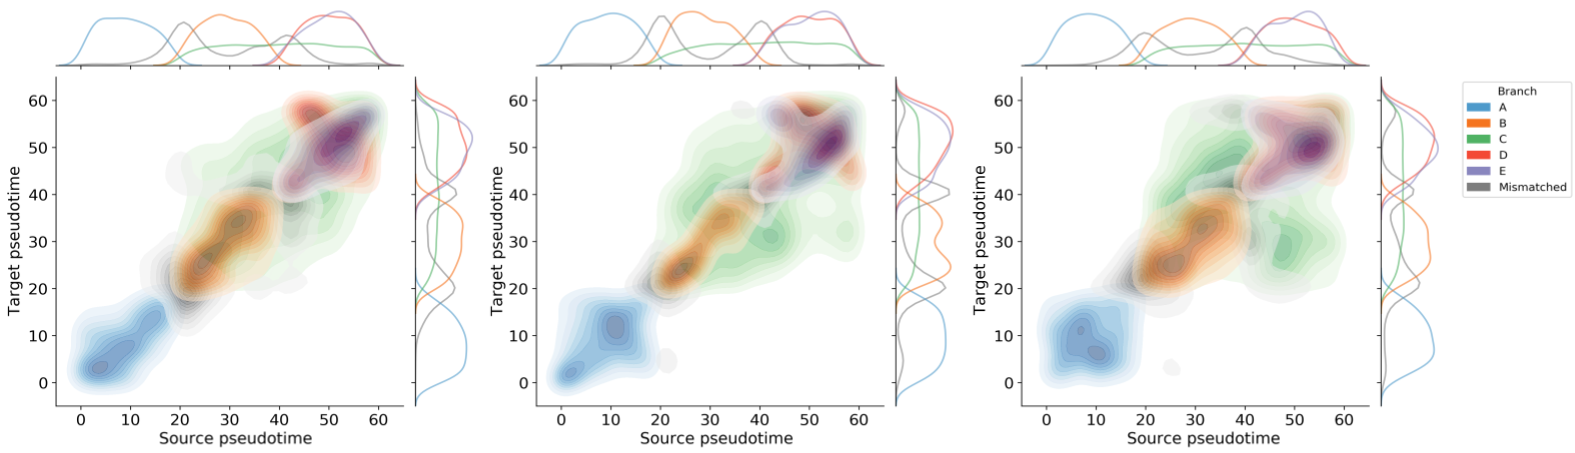
\includegraphics[width=1\textwidth]{figures/integration/3tech-pseudotime-kde.png}
%    \caption{
%    Evaluation of cross-technology cell matches made by SCIM on the simulated data with three technologies. 
%    The pairwise matching is attained for Source-Target A, Source-Target B, and Target A-Target B, respectively. The sink edge capacities were unbounded in all cases.
%    Here, we show a density plot for matched pseudotime values between the source technology and the target technology,
%    colored by the branch label. Mismatched cells are colored in grey.
%    The tree defining the temporal branching process can be found in Figure 3, left.
%    Marginal distributions of cell pseudotime for each branch is shown on the top and right.
%    }
%    \label{fig:prosstt5-3tech-pseudotime}
%\end{figure*}

The SCIM framework can be applied to a many-technology setting, and we demonstrate this by obtaining pairwise matches between all three datasets. 
SCIM successfully aligns the cells, based on evaluations on pseudotime (Supplemental Figure \ref{fig:prosstt5-3tech-pseudotime}) as well as branch label (Supplemental Tables \ref{tbl:prosstt_conf_SB} and  \ref{tbl:prosstt_conf_AB}), even when using codes from such an extended latent space. 

%\begin{table}[ht]
%\centering
%\begin{tabular}{lrrrrr}
%\toprule
%Target B &     A &     B &      C &     D &     E \\
%Source &       &       &        &       &       \\
%\midrule
%A      &  8,833 &   430 &    709 &     1 &     0 \\
%B      &   249 &  6,710 &    536 &   526 &   681 \\
%C      &   925 &   552 &  19,275 &     5 &     0 \\
%D      &     0 &   326 &      2 &  7,906 &   314 \\
%E      &     0 &   382 &      0 &   742 &  7,523 \\
%\bottomrule
%\end{tabular}
%\caption{Confusion table showing branch labels of the optimal matches of cells in the simulated PROSST data, between Source and Target B. Entries on the diagonal correspond to correct matches whereas off-diagonal elements to mismatches. The overall accuracy, with respect to the branch label, equals 89\%.}
%\label{tbl:prosstt_conf_SB}
%\end{table}

These results demonstrate that SCIM is capable of accurately identifying the best matching cells across multiple technologies, based on the shared latent representations in the presence of an underlying branching process but in the absence of paired features.

\subsection{Comparison to MATCHER}
We compare SCIM to MATCHER \citep{welch2017}, which is, to the best of our knowledge, the only other published work that can integrate multi-modal 'omics datasets in the absence of direct feature correspondences.
MATCHER, however, assumes a one-dimensional latent structure that struggles to capture hierarchical relationships, such as the ones exhibited in the simulated PROSSTT data, and frequently found and studied in single-cell datasets.
Moreover, MATCHER is built around a GPLVM \citep{lawrence2004}, which limits its scalability.
To this end, we set a budget of 48 hours compute time and limit memory consumption to 40 Gb.
Using the latent representations generated by MATCHER, we solve the bipartite matching problem setting the same hyperparameter configuration.
MATCHER is unable to model the PROSSTT branching structure and is outperformed by SCIM with respect to matching (see Supplemental Table  \ref{tbl:prosstt_matcher} and Supplemental Figure \ref{fig:prosstt5-matcher-psuedotime}).

%\begin{table*}%[H]
%\begin{tabular}{l|llllll}
%\toprule
%  method & accuracy & \#null matches & Spearman & Pearson \\
%\midrule
% SCIM    &   86\% &  1,590  & 0.83  & 0.86\\
% MATCHER &   4\%  & 25,510  & -0.21 & -0.19\\
%\bottomrule
%\end{tabular}
%\caption{The matching results on the PROSSTT dataset, where the SCIM matching algorithm was applied to SCIM shared latent codes and the MATCHER latent representation. The table depicts accuracy with respect to branch label, null node matches and the correlation coefficients for the pseudotime between matched source and target cells.}
%\label{tbl:prosstt_matcher}
%\end{table*}

%\begin{figure*}[htp]
%    \centering
%    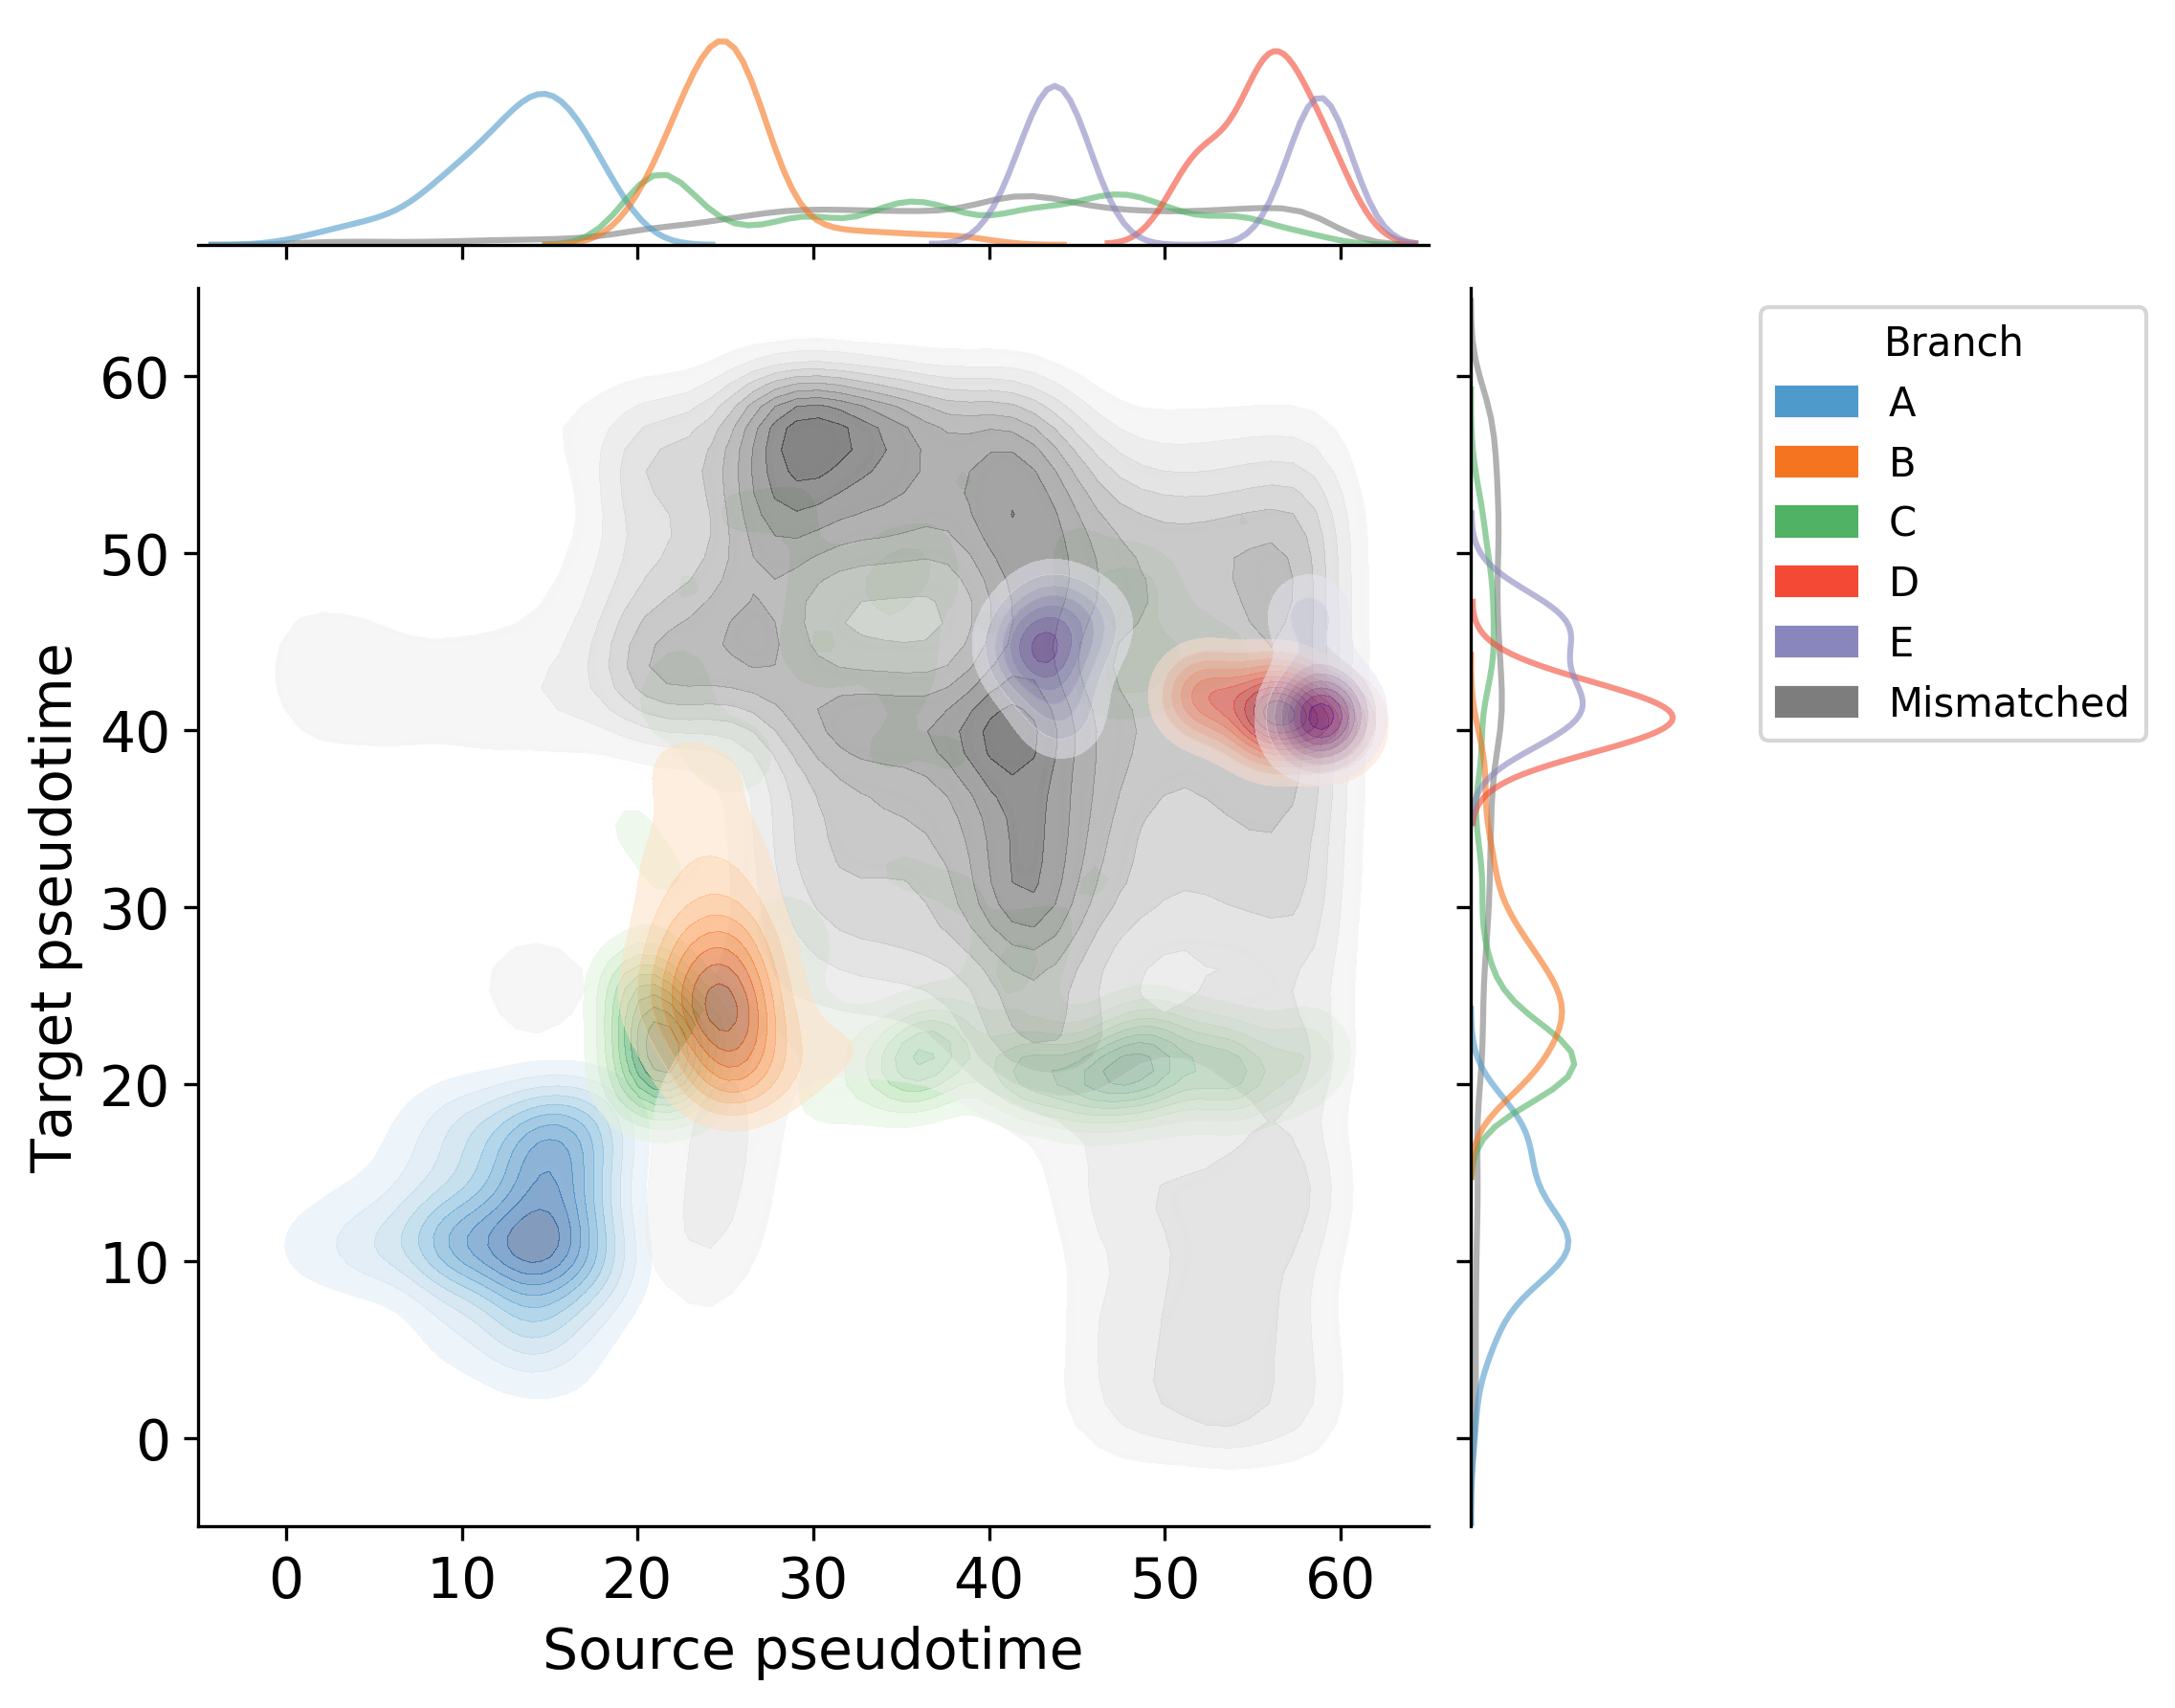
\includegraphics[width=1.0\textwidth]{figures/integration/matcher-pseudotime-kde.png}
%    \caption{
%    Evaluation of cross-technology cell matches using latent representation obtained by MATCHER on the simulated data.
%    Cells are matched across datasets pairwise using the bipartite matching scheme.
%    Here we show a density plot for matched pseudotime values between the source technology and the target technology,
%    colored by the branch label. Mismatched cells are colored in grey.
%    Marginal distributions of cell pseudotime for each branch are shown on the top and right.
%    }
%    \label{fig:prosstt5-matcher-psuedotime}
%\end{figure*}

\section{Integrating scRNA-seq and CyTOF profiles}


We apply SCIM to integrate two sets of scRNA/CyTOF data,
one set corresponds to a melanoma tumor from the Tumor Profiler project \cite{Irmisch2020}
and the other one to a human bone marrow sample from \citet{Oetjen2018}.
The scRNA technology was chosen both times as the source technology, and the latent space is initialized by training a VAE.
SCIM is trained for 64 epochs to integrate the CyTOF technologies.
The discriminator is trained in both cases to classify the source technology.
We employed a semi-supervised strategy and use only 10\% of the cell-type labels to help orienting the latent space.
Bipartite matching is performed in both cases using $k=50$ and a null match penalty set to the $95^{th}$ percentile of edge costs.


\subsection{Integration of a melanoma sample}
A major motivation for this work is derived from the setting of the Tumor Profiler (TuPro) Consortium \cite{Irmisch2020}.
This multi-center, multi-cancer study peforms a deep phenotyping of metastatic tumors from a real-life cohort, 
analyzing each sample with multiple technologies, including scRNA-sequencing \cite{Tang2009} and Cytometry by Time Of Flight \cite[CyTOF]{Bandura2009},
all of which are capable of dissecting the tumor microenvironment and providing single-cell level, complementary information about the sample of interest.
Although cell identity is lost throughout the experimental process, the cells profiled by both technologies stem from the same population
(i.e., were obtained from an aliquot of a common cell suspension), and can be thought of as being sampled from the same distribution of cells.

Here, we consider a melanoma sample from this study, and use SCIM to integrate CyTOF and scRNA-seq measurements to produce a more holistic cellular profile.

\subsubsection{Data Preparation}
\paragraph{CyTOF}
The patient's sample was profiled with CyTOF using a 41-markers panel designed for an in-depth characterization of the immune compartment of a sample.
Data preprocessing was performed following the workflow described in \cite{Chevrier2017, Chevrier2018}.
Cell-type assignment was performed using a Random Forest classifier trained on multiple manually gated samples.
To investigate the utility of SCIM, we considered a subset comprising B-cells and T-cells only, for a total of $n{=}135,334$ cells (\textbf{Table \ref{tbl:tupro-dataset}}).
This dataset is further referred to as \textit{target} dataset.

\paragraph{scRNA}
A second aliquot of the same patient sample was analyzed by droplet-based scRNA-sequencing using the 10x Genomics platform.
A detailed description of the data analysis workflow is beyond the scope of this work and will be published elsewhere.
In brief, standard QC-measures and preprocessing steps, such as removal of low quality cells, as well as filtering out mitochondrial, ribosomal and non-coding genes, were applied.
Expression data was library-size normalized and corrected for the cell-cycle effect.
Cell-type identification was performed using a set of cell-type-specific marker genes \cite{Tirosh2016}.
Genes were then filtered to retain those that could code for proteins measured in CyTOF channels, the top 32 T-cell / B-cell marker genes, and the remaining most variable genes for a final set of 256.
The total number of B-cells and T-cells in this dataset amounts to $m{=}4,683$ (\textbf{Table \ref{tbl:tupro-dataset}}).
The scRNA dataset is used as \textit{source} dataset throughout the manuscript.

\begin{table}[ht]
    \centering
    \begin{tabular}{lrrrr}
    \toprule
    Dataset &  \# Markers &  \# Cells &  T Cells &  B Cells \\
    \midrule
    CyTOF &         41 &   135,334 &       70\% &       30\% \\
    scRNA &       256 &     4,683 &       73\% &       27\% \\
    \bottomrule
    \end{tabular}
    \caption{
        Characteristics of the preprocessed dataset derived from the melanoma sample.
    }
    \label{tbl:tupro-dataset}
\end{table}

\subsubsection{Model selection}
\paragraph{Autoencoders}
The training procedure for SCIM's autocoders is goverened by an adversarial loss function.
Model selection in this setting with real-world data is challenging since, as there is no metric that captures model performance, nor is there access to some ground truth data with which to evaluate.
To facilitate model selection, we employ a universal divergence estimator \cite{Wang2009} to evaluate the quality of the integrated latent space (Figure\textbf{\ref{fig:tupro-train}}).

This score measures how well two sets of points are mixed and it is computed pairwise between source and target technologies.
An optimization is defined as successful if the divergence and reconstruction errors are below the empirically set thresholds.
This allows the evaluation of many model settings at scale despite operating in the adversarial setting.
We find that performance depends on tuning $\beta$ and the learning rates for the discriminator and encoder/decoder networks (see \textbf{Table~\ref{tbl:ablation_menytek}}).

\begin{figure*}[htbp]
    \centering
    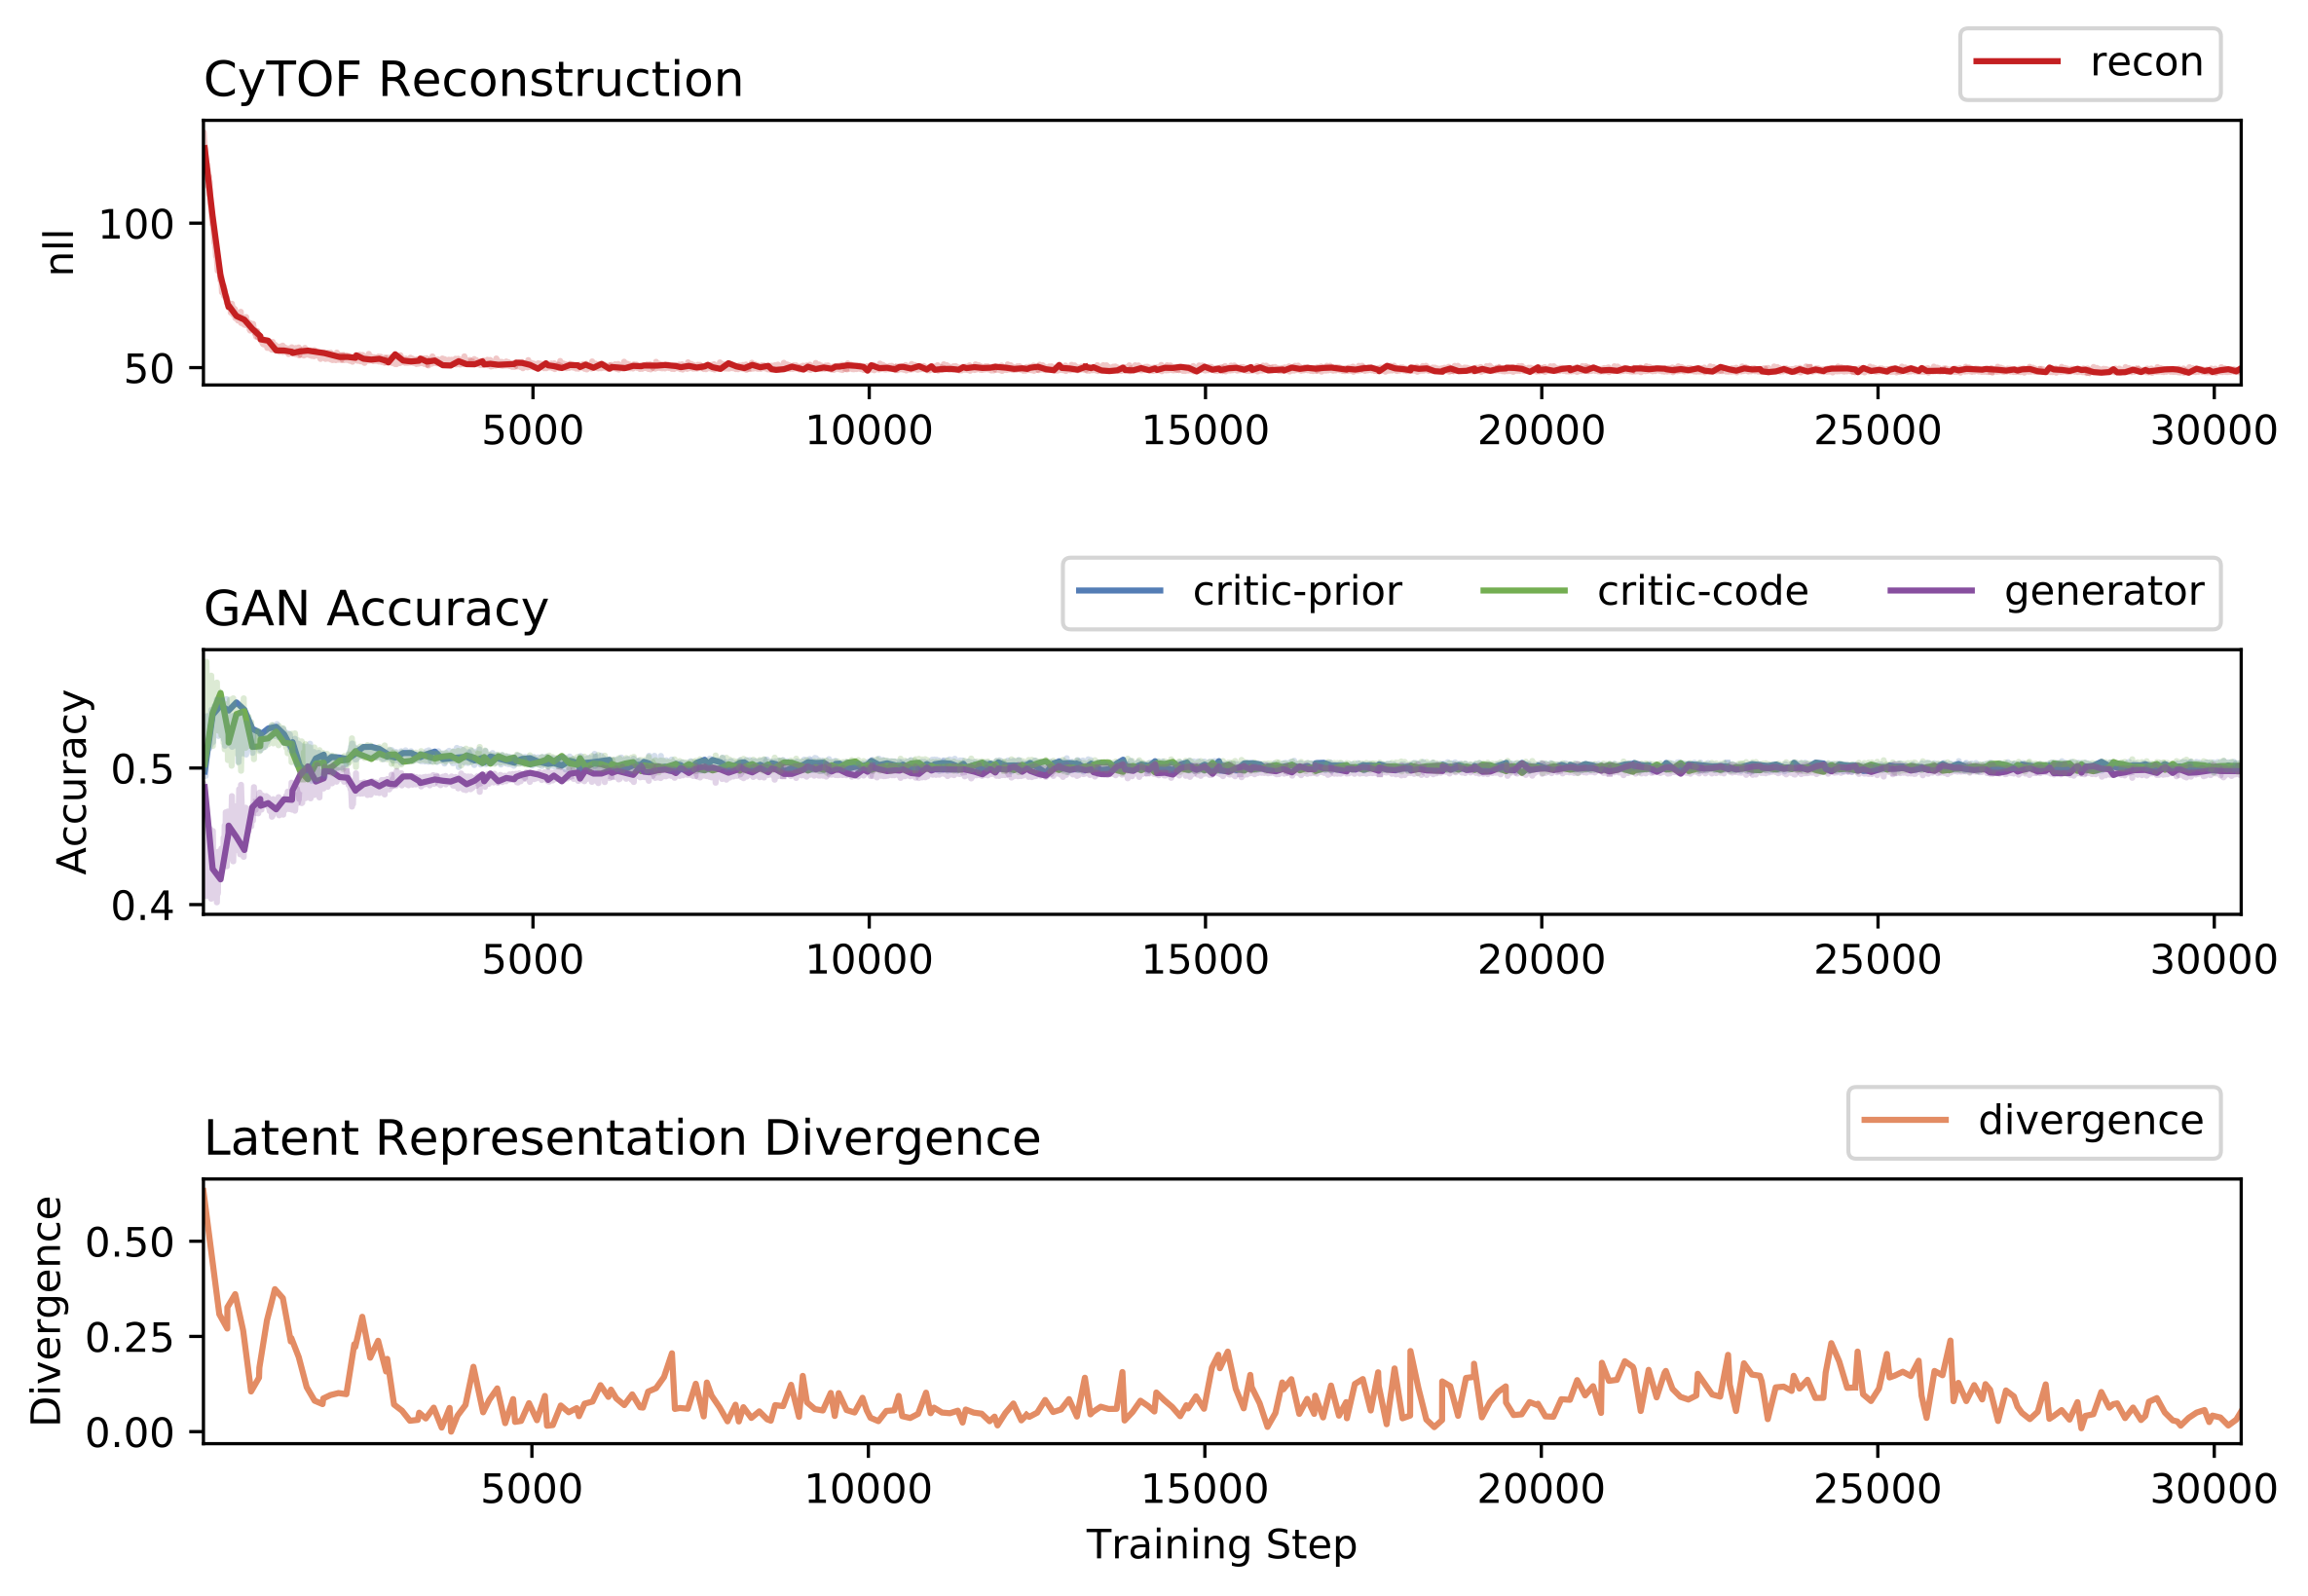
\includegraphics[width=0.95\textwidth]{figures/integration/menytek-train-scores}
    \caption{
        Training progress of SCIM on a melanoma sample.
        The latent space is initialized by training a VAE on scRNA data.
        SCIM integrates CyTOF representations into the latent space
        defined by the scRNA codes.
        The top panel shows the negative log-likelihood of the CyTOF reconstruction.
        The middle panel shows the performance of the discriminator to correctly classify scRNA codes (critic-prior), CyTOF codes (critic-code), and the ability of the encoder to fool the discriminator, i.e., the misclassification accuracy (generator).
        The bottom panel shows the divergence of the latent representations.
        The model is able to converge quickly.
However, the divergence score can fluctuate despite still fooling the discriminator.
        Training took 2h 10min and had a peak memory consumption of 1068 MB.
    }
    \label{fig:tupro-train}
\end{figure*}

\begin{table}[h]
\centering
\begin{tabular}{rrrrrr}
\toprule
Censor & $\beta$ &  ${lr}_{\phi,\psi}$&  ${lr}_\gamma$ & Success &  \# runs \\
\midrule
0.00 &      16 &            0.0010 &  0.0010 &         14\% &           7 \\
     &      16 &            0.0010 &  0.0005 &         14\% &           7 \\
     &      16 &            0.0005 &  0.0005 &         10\% &          10 \\
     &      16 &            0.0005 &  0.0010 &         10\% &          10 \\
0.25 &      16 &            0.0010 &  0.0010 &         14\% &          14 \\
     &      16 &            0.0005 &  0.0010 &         12\% &          17 \\
     &      64 &            0.0001 &  0.0005 &          0\% &           7 \\
     &      64 &            0.0001 &  0.0010 &          0\% &           7 \\
0.75 &      16 &            0.0005 &  0.0010 &         17\% &           6 \\
     &      32 &            0.0005 &  0.0005 &         12\% &           8 \\
     &      16 &            0.0010 &  0.0005 &          8\% &          13 \\
     &      64 &            0.0001 &  0.0005 &          0\% &           7 \\
0.90 &      16 &            0.0005 &  0.0010 &         40\% &          10 \\
     &      16 &            0.0010 &  0.0005 &         10\% &          10 \\
     &      16 &            0.0005 &  0.0005 &          8\% &          12 \\
     &      32 &            0.0010 &  0.0001 &          0\% &          10 \\
0.95 &      32 &            0.0010 &  0.0001 &          0\% &           4 \\
     &      64 &            0.0001 &  0.0005 &          0\% &           4 \\
     &      64 &            0.0001 &  0.0010 &          0\% &           6 \\
     &      32 &            0.0010 &  0.0010 &          0\% &           5 \\
0.99 &      16 &            0.0005 &  0.0010 &         17\% &           6 \\
     &      32 &            0.0010 &  0.0005 &          0\% &           6 \\
     &      64 &            0.0001 &  0.0005 &          0\% &           4 \\
     &      32 &            0.0010 &  0.0001 &          0\% &           6 \\
\bottomrule
\end{tabular}
\caption{
    Ablation study for training SCIM on the melanoma patient at several levels of semi-supervision.
    Fraction censored is the fraction of labels removed during training.
    The top 4 configurations for each level of semi-supervision is shown.
    $\beta$ is the regularization strength of the adversarial loss.
    Learning rates are the initial settings of the ADAM optimizer.
    If the latent space divergence is below 0.3 and
    the negative log-likelihood of the input under the reconstruction is below 47,
    the training is determined to be a success. These values were chosen empirically.
    We see that $\beta$ and optimizer learning rates were heavily influential on model success.
}
\label{tbl:ablation_menytek}
\end{table}

\paragraph{Bi-partite matching is scalable}
Due to the large number of cells profiled with each individual technology per sample, we precede our bipartite matching with a kNN search.
This reduces the problem complexity by \textit{a priori} discarding redundant edges in the graph.
Experiments on the real-world melanoma sample investigating the level of sparsity, governed by a hyperparameter \textit{k}, show that using even a small number of neighbors provides good matching accuracy and performance saturates past $k>100$ (see \textbf{Supplemental Figure~\ref{fig:matching_accuracy_log10_uni}}, \textbf{Supplemental Table~\ref{tbl:menytek_tune_k_uni}}).
This is in line with our expectations since a match to an extremely distant neighbor is hard to justify.
In order to maintain a high degree of sparsity, without sacrificing matching accuracy, we use $k=50$ in all further experiments.

\begin{figure*}[h]
    \centering
    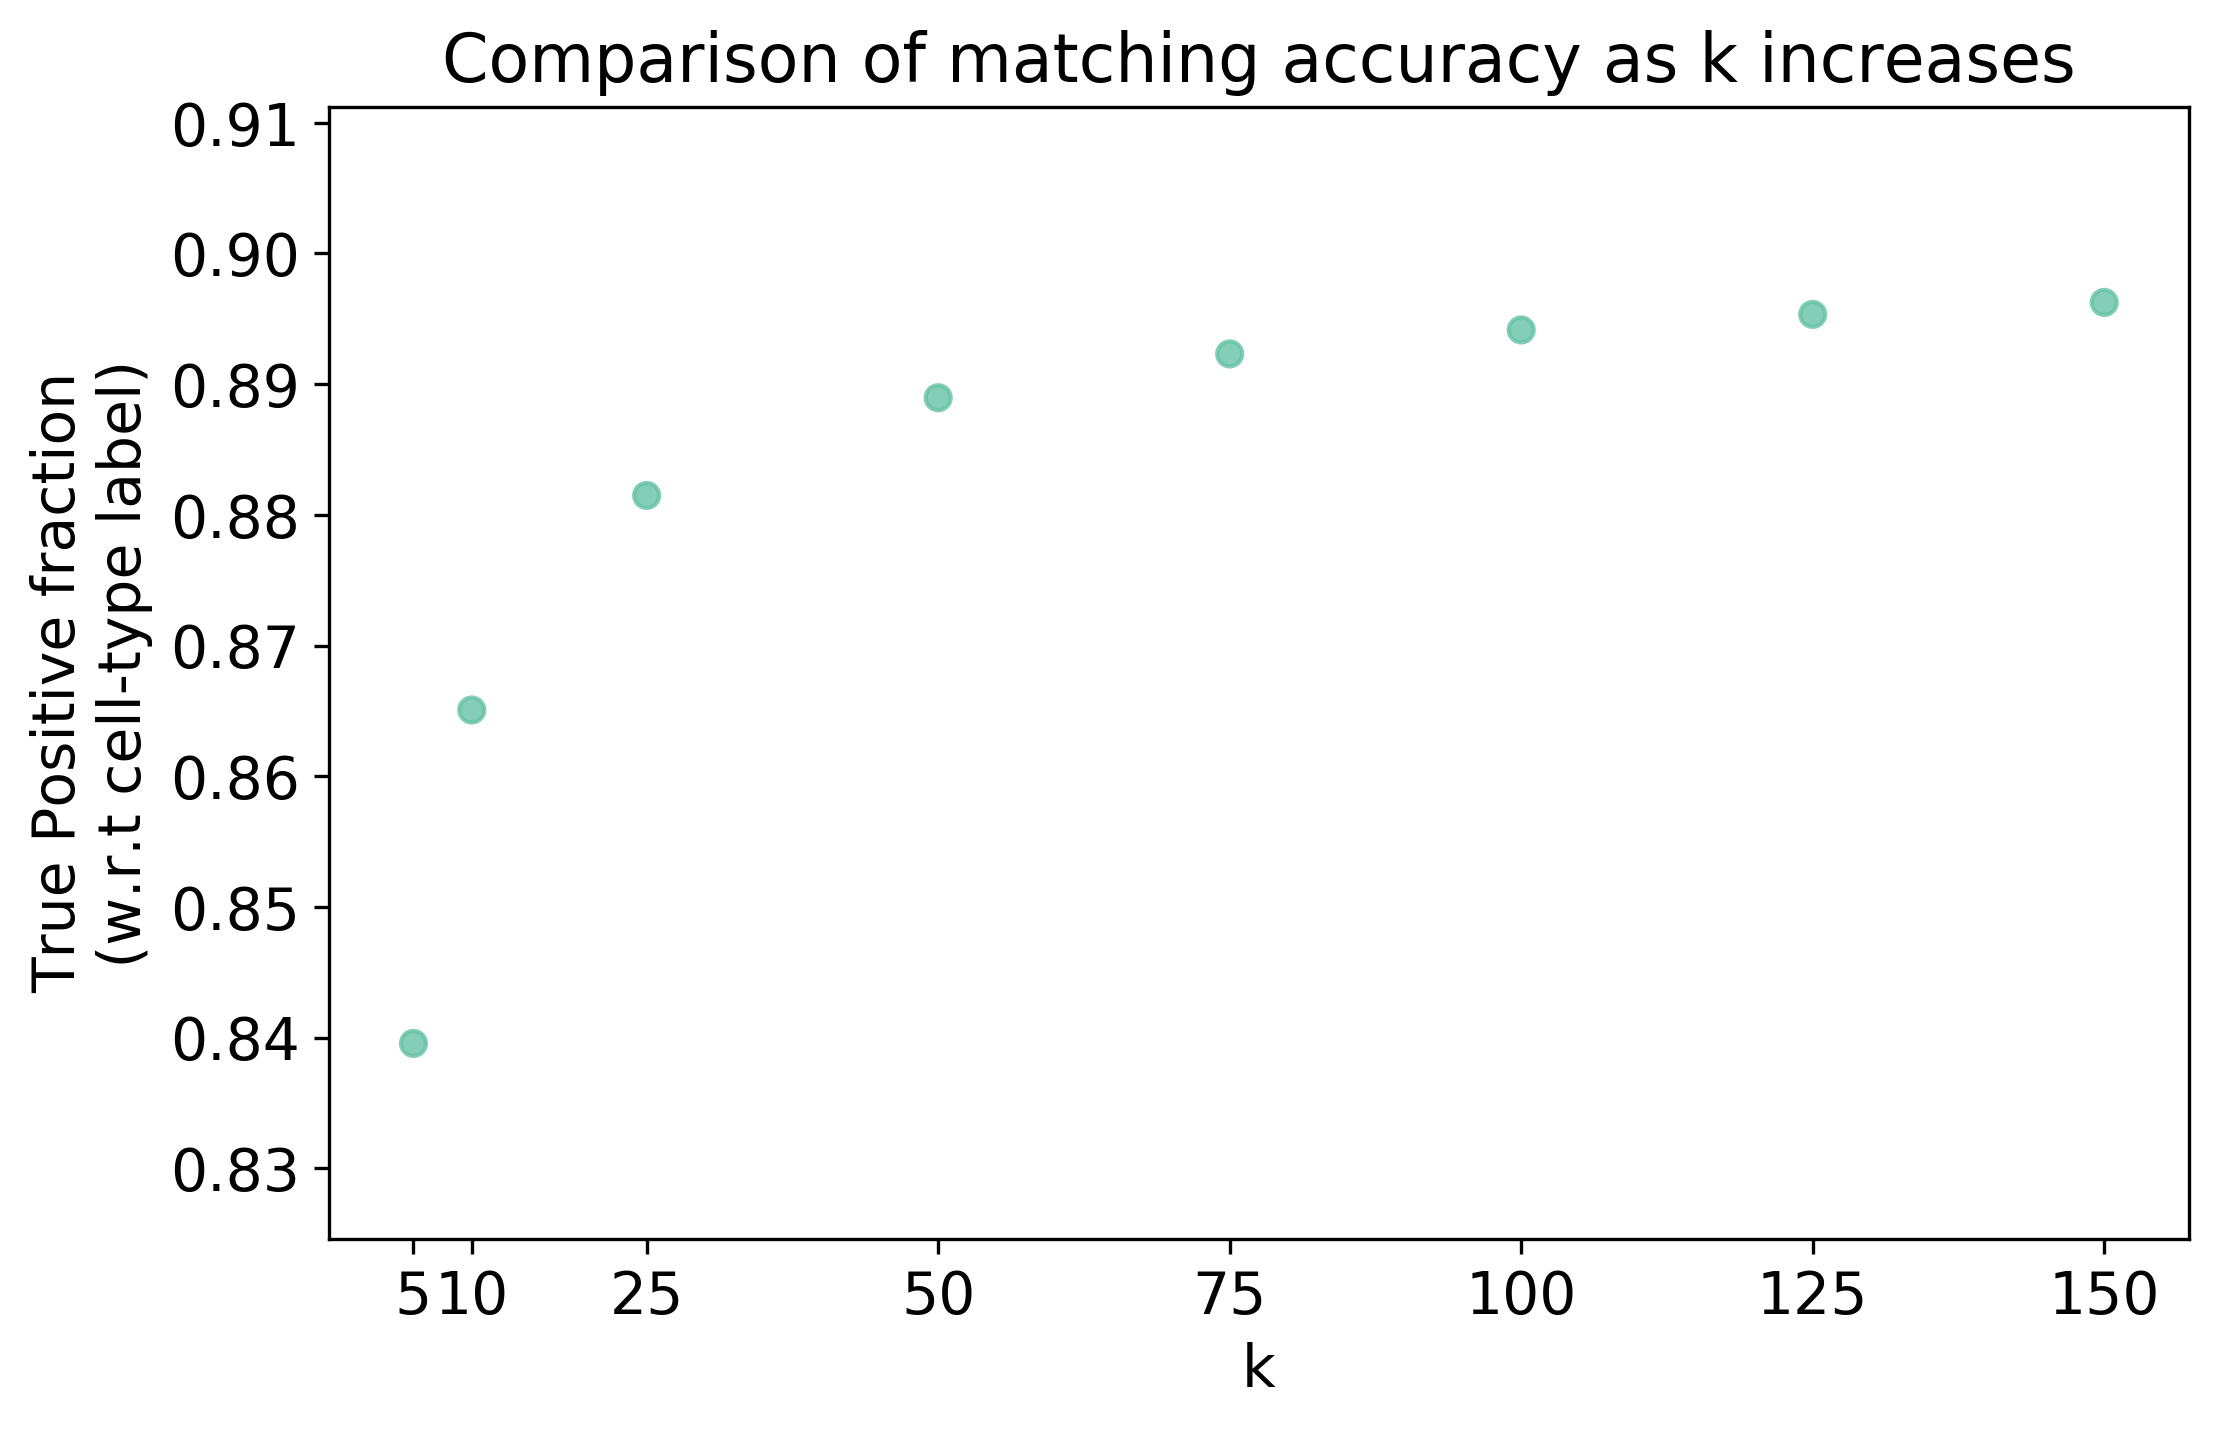
\includegraphics[width=0.85\textwidth]{figures/integration/matching-tune-k-unicapacity.png}
    \caption{Comparison of matching accuracy, with respect to cell-type label as less sparsity of connections, is imposed on the Tumor Profiler data.
The number of considered Nearest Neighbors \textit{k} is indicated on the x-axis, and the fraction of true positive matches, with respect to cell-type label, is depicted on the y-axis.
 The accuracy level saturates with $k=100$.}
    \label{fig:matching_accuracy_log10_uni}
\end{figure*}

\begin{table*}[h]
\centering
\begin{tabular}{lrr}
\toprule
{} &  CPU time [s] &  Max Memory [Mb] \\
k   &               &                  \\
\midrule
5   &       1,492.67 &          1,674.94 \\
10  &       2,803.33 &          2,456.27 \\
25  &       7,723.67 &          4,690.05 \\
50  &       7,441.33 &          8,740.34 \\
75  &      12,656.00 &         12,344.52 \\
100 &      17,331.00 &         17,002.75 \\
125 &      26,047.00 &         20,612.78 \\
150 &      33,718.00 &         24,222.75 \\
\bottomrule
\end{tabular}

\caption{Memory usage and computation time of the bipartite matching as \textit{k} hyperparameter in kNN search increases.
The values were obtained on the whole TuPro dataset using the MCMF algorithm on an extended graph. %, as described in section \ref{graph_extensions}.
The cost of matching to the null node was set to 95th percentile, and a union of connections obtained from kNN graphs with \textit{k} indicated in the first column was used for matching.
The memory and time reports were averaged across three independent runs.}
\label{tbl:menytek_tune_k_uni}
\end{table*}

\subsection{SCIM Pairs Cells Across scRNA and CyTOF in a Melanoma Sample}
The bipartite matching on the latent codes has a 90\% accuracy in recovering the cell-type label, calculated as the fraction of true positives over all matches.
A more fine-grained visual evaluation is performed by inspecting the matches on a tSNE embedding of the integrated latent space marked by grey lines (see \textbf{Figure~\ref{fig:tupro-tsne-uni}}).
Given different cell-type proportions in the data, a certain number of mismatches is expected, which corresponds to the lines joining points across the two cell types.
The latent representation is explored thoroughly as 98\%, and 99.9\% of cells are matched to their analogs, from CyTOF and scRNA datasets, respectively.
To evaluate the latent space matching further, we used a more fine-grained information of marker expression correlation, to quantitatively assess the latent-space matching quality.
We used the correlation coefficients between the expression of immunomarkers \textit{CD20} and \textit{CD3}.
Both markers are characteristic for a subset of our data, as they are used to differentiate B-cells and T-cells, respectively.
We found that matching using shared latent representations provides relatively high correlation coefficients
(Pearson: 0.63 \textit{CD20} and 0.51 for \textit{CD3} marker, see \textbf{Supplemental Figure~\ref{fig:tupro-marker-correlation-uni}}),
given the expected low correlation between RNA expression and protein abundance.

\begin{figure*}[htbp]
    \centering
    \includegraphics[width=0.95\textwidth]{figures/integration/tsne-matched-unicapacity.png}
    \caption{
    Integrated latent space and matches of scRNA and CyTOF cells from a melanoma sample from the Tumor Profiler Consortium.
    Discriminators are semi-supervised using 10\% of the cell-type labels.
    Cells are colored by their cell-type label and shaded by their technology (dark shades: CyTOF, light shades: scRNA).
    Matches produced by SCIM are represented by grey lines connecting cells.
    tSNE embeddings \cite{Maaten2008} are computed on the whole dataset and then 10,000 matched pairs are sampled at random for visualization.}
    \label{fig:tupro-tsne-uni}
\end{figure*}


\begin{figure*}[htbp]
    \centering
    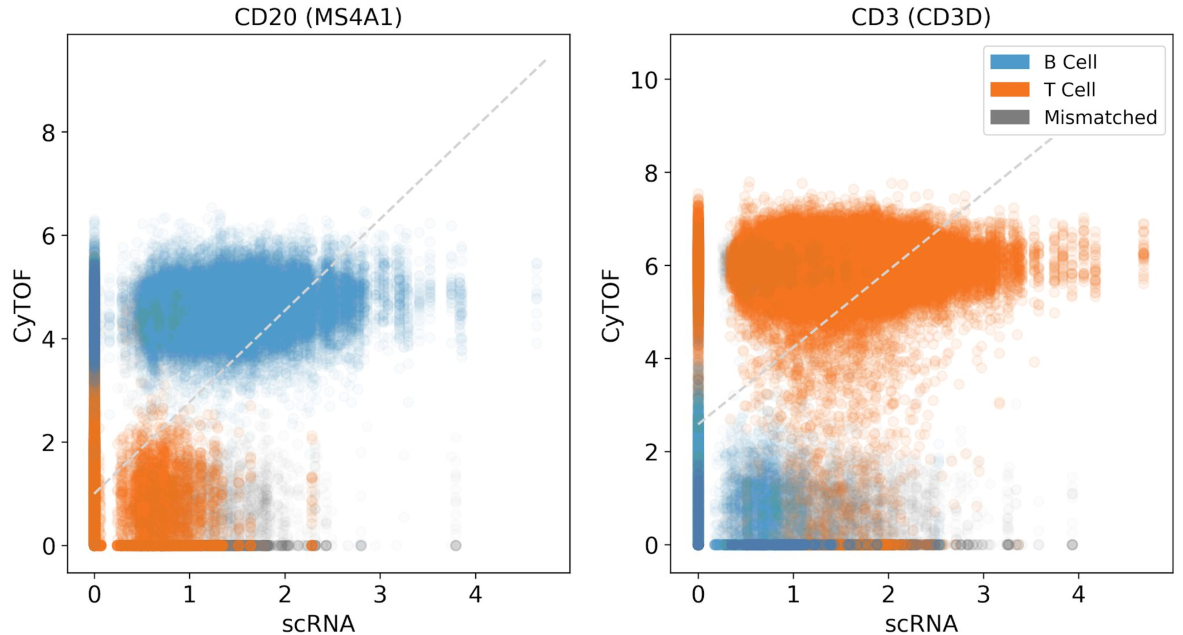
\includegraphics[width=0.65\textwidth]{figures/integration/gene_protein_correlation_unicapacity}
    \caption{
      \textit{CD20} and \textit{CD3} marker abundances measured with scRNA (gene, x-axis) and CyTOF (protein, y-axis) in a melanoma sample from the Tumor Profiler Consortium.
      The values on the axes represent normalized expression.
      Colors (blue, orange) represent cell types (B-cell, T-cell) while grey marks mismatches with respect to the cell-type label.
      The linear regression line is depicted by a dashed light grey line.
      Pearson's correlation coefficient equals 0.63 and 0.51 for CD20 and CD3, respectively.
      Spearman's correlation coefficient amounts to 0.55 and 0.42, for CD20 and CD3, respectively.
    }
    \label{fig:tupro-marker-correlation-uni}
\end{figure*}


\subsection{Integration of a human bone marrow sample}
\cite{Oetjen2018} used several bulk and single-cell technologies to comprehensively characterize human bone marrow.
The data was obtained from 20 healthy donors, whereas all data modalities were acquired for 8 samples.
For our application we consider the single-cell transcriptome profile as well as CyTOF measurements of sample \textit{O} from this dataset, that were carried out with the objective of describing in detail a T-cell~population.
The data was preprocessed as described in \cite{Oetjen2018}.
A subpopulation of CD8 naive T-cells was filtered out due to a very small number of cells.
The preprocessed data of the analysed sample included several T-cell~subtypes (\textbf{Table~\ref{tbl:oetjen-dataset}}).

\begin{table}[h]
    \centering
    \begin{tabular}{lrrrrr}
    \toprule
    Dataset &  \# Markers &  \# Cells &  CD8 effector &  CD4 naive & CD4 memory  \\
    \midrule
    CyTOF &         34 &   98,799 &       57\% &       26\% & 17\% \\
    scRNA &       256 &     2,388 &       46\% &       31\% & 23\% \\
    \bottomrule
    \end{tabular}
    \caption{
        Characteristics of the preprocessed dataset derived from the human bone marrow sample. 
    }
    \label{tbl:oetjen-dataset}   
\end{table}

We use SCIM to integrate T-cells~derived from one sample in the Human Bone Marrow study, profiled with scRNA and CyTOF technologies.
The tSNE embedding based on the latent space codes implies good integration across technologies while preserving the cell-subtype structure \textbf{Supplemental Figure~\ref{fig:oetjen_tsne_uni}}.
We evaluate the quality of matches using fine-grained labels indicating one of the T-cell subtypes identified in gating: CD8 effector, CD4 naive, CD4 memory.
In a fully supervised approach, using the labels to orient the latent space, we achieve an accuracy of $83\%$ with  less than $8\%$ of matches directed to the null node.
Nevertheless, when utilizing only $10\%$ of the labels in the semi-supervised approach, we note only a slight drop in performance, obtaining $78\%$ correct matches with less than $8\%$ of cells directed to the null node.
Evaluating on higher-level labels of CD8 vs.
CD4 T-cells~improves the accuracy to $91\%$ and $86\%$ for the fully supervised and semi-supervised approach, respectively.
As expected, distinguishing cellular subtypes (e.g., CD4 naive versus CD4 memory) is more challenging due to high similarity between the cell populations, but overall SCIM is capable of accurately recovering even such subtle differences between cell types and states.

\begin{figure*}[htb]
    \centering
    \includegraphics[width=0.85\textwidth]{figures/integration/oetjen-tsne-matched-unicapacity.png}
    \caption{
    A tSNE embedding (perplexity=30) of the integrated latent space with cell matches indicated by the grey lines.
    The shared representation was obtained in a semi-supervised fashion, utilizing 10\% of the cell-type labels to orient the latent space. 10,000 matched pairs were sampled at random for the plot.
    Colors (blue, green, orange) represent T-cell subtypes (CD8 effector, CD4 naive, CD4 memory), and color shades correspond to the profiling technology (light: scRNA, dark: CyTOF).}
    \label{fig:oetjen_tsne_uni}
\end{figure*}

\section{Discussion}
We have developed SCIM, a new technology-invariant approach that pairs single-cell measurements across multi-modal datasets, without requiring feature correspondences.
This development enables real multi-modal single-cell analysis, and opens up new opportunities to gain a multi-view understanding of the dynamics of individual cells in various disease or developmental states.
The underlying autoencoder framework, combined with a customized bipartite matching approach, ensures scalability even to large numbers of cells.
 
We demonstrate that our model performs well on simulated data as well as on real-world melanoma and bone marrow samples profiled with scRNA and CyTOF.
The SCIM framework is presented here on two and three data modalities and easily extends to additional technologies, providing a new and effective solution to the multi-level data integration problem.
Integration of Image Mass Cytometry \cite{giesen2014} or single-cell ATAC-seq data \cite{buenrostro2015} for example, could enable the spatial analysis of regulatory and global expression changes not just in cancer but also in other diseases such as multiple sclerosis, where detailed spatiotemporal information has already been shown to provide relevant insights \cite{ramaglia2019}.
Notably, SCIM allows for the integration of cell populations  undergoing branching processes, enabling the study of temporal phenomena, such as developmental and cell fate determination.
The scalability of our framework ensures applicability beyond single samples, facilitating the study of large cohorts or the integration of SCIM into analytical workflows.
 
As the low-dimensional representation of the data produced by SCIM is used solely to perform cell matching, it can be combined with any other analytical methods.
The truly observed signals per cell pair measured with different technologies can be used for any downstream analysis.
By adopting a divergence measure \cite{wang2009}, we addressed common constraints in adversarial training, such as training instability and convergence problems.
To ensure scalability, we used a modified bipartite matching solution to efficiently match corresponding cells across technologies.
Our extensions guarantee  wider applicability of SCIM, since shifts in cell-type composition across disjoint aliquots, even coming from the same sample, can be expected.
Furthermore, the introduction of the \textit{null} node ensures a higher quality of matches by avoiding forced mismatches and thus, improving confidence in the cell-to-cell assignments.

With increasing data dimensionality, the number of nearest neighbors (\textit{k}) should also rise, since more ties are likely to occur.
Nevertheless, the difference in the number of true positives across various values of \textit{k} for the same dataset remains within 6\% in our experiments.
Hence, we can state that performance is robust against the choice of this hyperparameter.
Depending on the actual data, bounded or unbounded edge capacities (nearest neighbor approach) may be preferable.
Furthermore, SCIM is itself inherently modular, and other matching strategies that may be more suitable to other data types or experimental designs can be easily deployed on the integrated latent codes.

SCIM helps bridge the gap between data generation and integrative interpretation of diverse multi-modal data in the rapidly expanding field of single-cell biology, providing users with an easily scalable algorithm designed to maximize the information it provides and not limited to fit a particular analytical approach.

\paragraph{Current state-of-the-art}
While SCIM was among the first instances of a method designed and applied to the integration of multi-modal single-cell datasets, many other methods have emerged since its publication.
Many of these methods address the fact that while feature correspondences between single-cell modalities may be weak,  they are not totally absent, and introduce some modeling capability to utilize information that relates cross-modal features. 
Furthermore, in 2021, as part of that year NeurIPS conference, \citeauthor{lance2022} organized a competition that included single-cell multi-modal integration tasks such as the imputation or alignment of missing modalities and the learning of multi-modal cellular representations.
This competition helped bring the integration problem into the attention of the machine learning community and many methods and approaches were released around the time of this event.
Here a few promising and emerging methods are highlighted.
GLUE \cite{cao2022a}, and its extension CLUE \cite{tu2022}, which was awarded as a winner in the NeurIPS competition,
utilize a multi-modal VAE framework, like SCIM, but utilize knowledge graphs to help incorporate a notion of cross-modality feature correspondences.
Recently, \citeauthor{samaran2024} introduced a multi-modal integration framework utilizing optimal transport to help enforce feature correspondences.
This framework is also based on unpaired, modality specific auto-encoders, but uses a modality pairwise optimal transport coupling between a subset of shared features to help regularize and align the construction of the latent space.

\paragraph{Impact} Despite the emergence of other methods, the modeling approach taken by SCIM has proven to be influential in independent analyses of multimodal single-cell datasets. 
\citeauthor{fleck2023} and \citeauthor{wahle2023} adapted the SCIM framework in their respective multi-modal analyses of brain and retinal organoids.
These authors substitute the auto-encoder framework with the more simple canonical correlation analysis in order to construct an integrated representation space across scRNA-seq and scATAC-seq data, then utilized a bi-partite matching to recover "multiomic metacells."
In a similar vein, \citeauthor{meier2023} studied the specification and differentiation of epicardioids in the development of heart tissue, under a multi-modal lens.
While they opted for the use of GLUE embeddings \cite{cao2022}, they modified its approach with a SCIM-inspired bi-partite matching scheme to finalize the integration.


\chapter{Learning to align single-cell perturbation responses} \label{ch:cellot}

\section{Introduction}
% TODO: major: rephrase

Characterizing and modeling perturbation responses at the single-cell level from non-time-resolved data remains one of biology's grand challenges.
It finds applications in predicting cellular reactions to environmental stress or a patient's response to drug treatments.
Accurate inference of perturbation responses at the single cell level allows us,
for instance, to understand how and why individual tumor cells evade cancer therapies \cite{frangieh2021multimodal}.
More generally, it deepens the mechanistic understanding of the molecular machinery that determines the respective responses to perturbations.
Single-cell responses to genetic or chemical perturbations are highly heterogeneous \cite{liberali2014hierarchical} due to multiple factors,
including pre-existing variability in the abundance and subcellular organization of mRNA and proteins \cite{battich2013image, battich2015control, gut2018multiplexed, shaffer2017rare},
cellular states \cite{kramer2019cellular}, and the cellular microenvironment \cite{snijder2009population}.
To effectively predict the drug response of each cell in a  population, whether derived from tissue culture or as primary cells from a patient biopsy,
it is thus crucial to incorporate this heterogeneous multivariate subpopulation structure into the analysis.

A fundamental difficulty in learning perturbation responses is that cells are usually fixed and stained or chemically destroyed to obtain these measurements.
Hence, it is only possible to measure the same cells  before or after a perturbation is applied.

Therefore, while we do not have access to a set of \emph{paired} control/perturbed single-cell observations, we do have access to separate \emph{sets} of single-cell observations from control and perturbed cells, respectively.
To subsequently match single cells between conditions and, at the same time, account for cellular heterogeneity is a highly complex pairing problem.

Here, we seek to learn a perturbation model that robustly describes the cellular dynamics upon intervention while still accounting for underlying variability across samples.
Learning the responses on an existing patient cohort enables inference of treatment responses for new, i.e., previously unseen patients,
assuming that we captured the heterogeneous drug reactions of patients during training.
It is crucial, however, to not simply model average perturbation responses of a patient cohort,
but to capture the specificities of a single patient through personalized treatment effect predictions.
% Even though we seek a robust and coherent model, we must ensure that we propose personalized treatment effect predictions rather than average perturbation responses of a patient cohort possibly not capturing the specificities of a single patient.

Previous methods to approximate single-cell perturbation responses fall short of solving this highly complex \emph{pairing} problem while, at the same time,
accounting for cellular heterogeneity and the strong subpopulation structure of cell samples \cite{wu2021single,gonzalez2020tumor,li2022single}.

Current state-of-the-art methods \cite{Lopez2018scvi, lotfollahi2019scgen, yang2020predicting} predict perturbation responses via \emph{linear shifts} in a learned % low-dimensional
latent space.
While this can capture nonlinear cell-type-specific responses, the use of linear interpolations reduces the alignment problem 
to the possibly more challenging task of learning representations that are invariant to the corresponding perturbation.


In this chapter, we introduce \textsc{CellOT}, a novel approach that predicts perturbation responses of single cells by \emph{directly} learning and uncovering maps 
between control and perturbed cell states, thus explicitly accounting for heterogeneous subpopulation structures in multiplexed molecular readouts.
Assuming perturbations incrementally alter molecular profiles of cells, such as gene expression or signaling activities,
we learn these changes and alignments using optimal transportation theory (OT) \cite{villani2009optimal}.
Optimal transport provides natural geometric and mathematical tools to manipulate probability distributions.
It has found recent successes modeling cellular development processes \cite{lavenant2021towards, schiebinger2019optimal},
albeit in a \emph{non-parameterized} setting.
Thus, current OT-based approaches are unable to make predictions on unseen cells, such as those from unseen samples, e.g., new patients.

% One way to address the pairing problem is to assume that perturbed cellular states are coupled to their initial states under a principle of minimum action.
That is, given unpaired observations of cells before and after perturbation,
we would aim to pair cells to their treated states in such a way that the average distance between the pairs, in feature space, is minimal.
This setting is ideally suited for acute cellular perturbations during which single cells do not redistribute entirely and randomly in multidimensional measurement space,
but typically only in a few dimensions, maintaining the overall correlation structure.

Based on recent developments in neural optimal transport \cite{makkuva2020optimal},
\textsc{CellOT} learns an optimal transport map for each perturbation in a fully parameterized and highly scalable manner.
Instead of directly learning a transport map \cite{jacob2018w2gan, yang2018scalable, prasad2020optimal},
\textsc{CellOT} parameterizes a pair of dual potentials with convex neural networks \cite{amos2017input}.
This choice induces an important theory-motivated inductive bias essential to model stability \cite{makkuva2020optimal}.


We demonstrate \textsc{CellOT}'s effectiveness biopsy
(i) learning single-cell marker responses to different cancer drugs in melanoma cell lines,
(ii) predicting single-cell transcriptome responses in biopsies of patients with systemic lupus erythematosus as well as Panobinostat treatment outcomes of glioblastoma patients,
(iii) inferring LPS responses across different animal species,
and (iv) modeling the transcriptome evolution of cell fates in hematopoiesis.
Moreover, we benchmark \textsc{CellOT} against current state-of-the-art methods on multiple tasks \cite{Lopez2018scvi, lotfollahi2019scgen}.

\section{Learning single-cell perturbation responses}
% TODO: finish
Popular approaches to model single-cell perturbation responses fall into three main camps, figure \ref{fig:arrows}.
The first takes a simple approach that ignores heterogeneity in response and models perturbations as linear shifts in data space, figure \ref{fig:arrows} left.
Cell typing approaches take this assumption, at least piece wise, and thus fail to capture any intra cell-type heterogeneity.
A popular approach is to model perturbation effects as a linear shift in some latent space that is then decoded with a non-linear function
These approaches include models like \textsc{scGen} \cite{lotfollahi2019} but many other models take similar approaches \cite{need}
While this approach is able to model heterogeneity, they need to implicitly solve a challenging disentanglement task \cite{locatello2018}, which, if not solved correctly, leads to aberrant behavior, figure \ref{fig:arrows} middle. 
In this work we opt to use a modern parameterization of an optimal transport coupling, figure \ref{fig:arrows} right.
Thanks to the mathematics of optimal transport, this allows us to predict treated states accurately by following a strict adherence to the control and treated distribution geometries.

\begin{figure}[ht]
  \begin{center}
    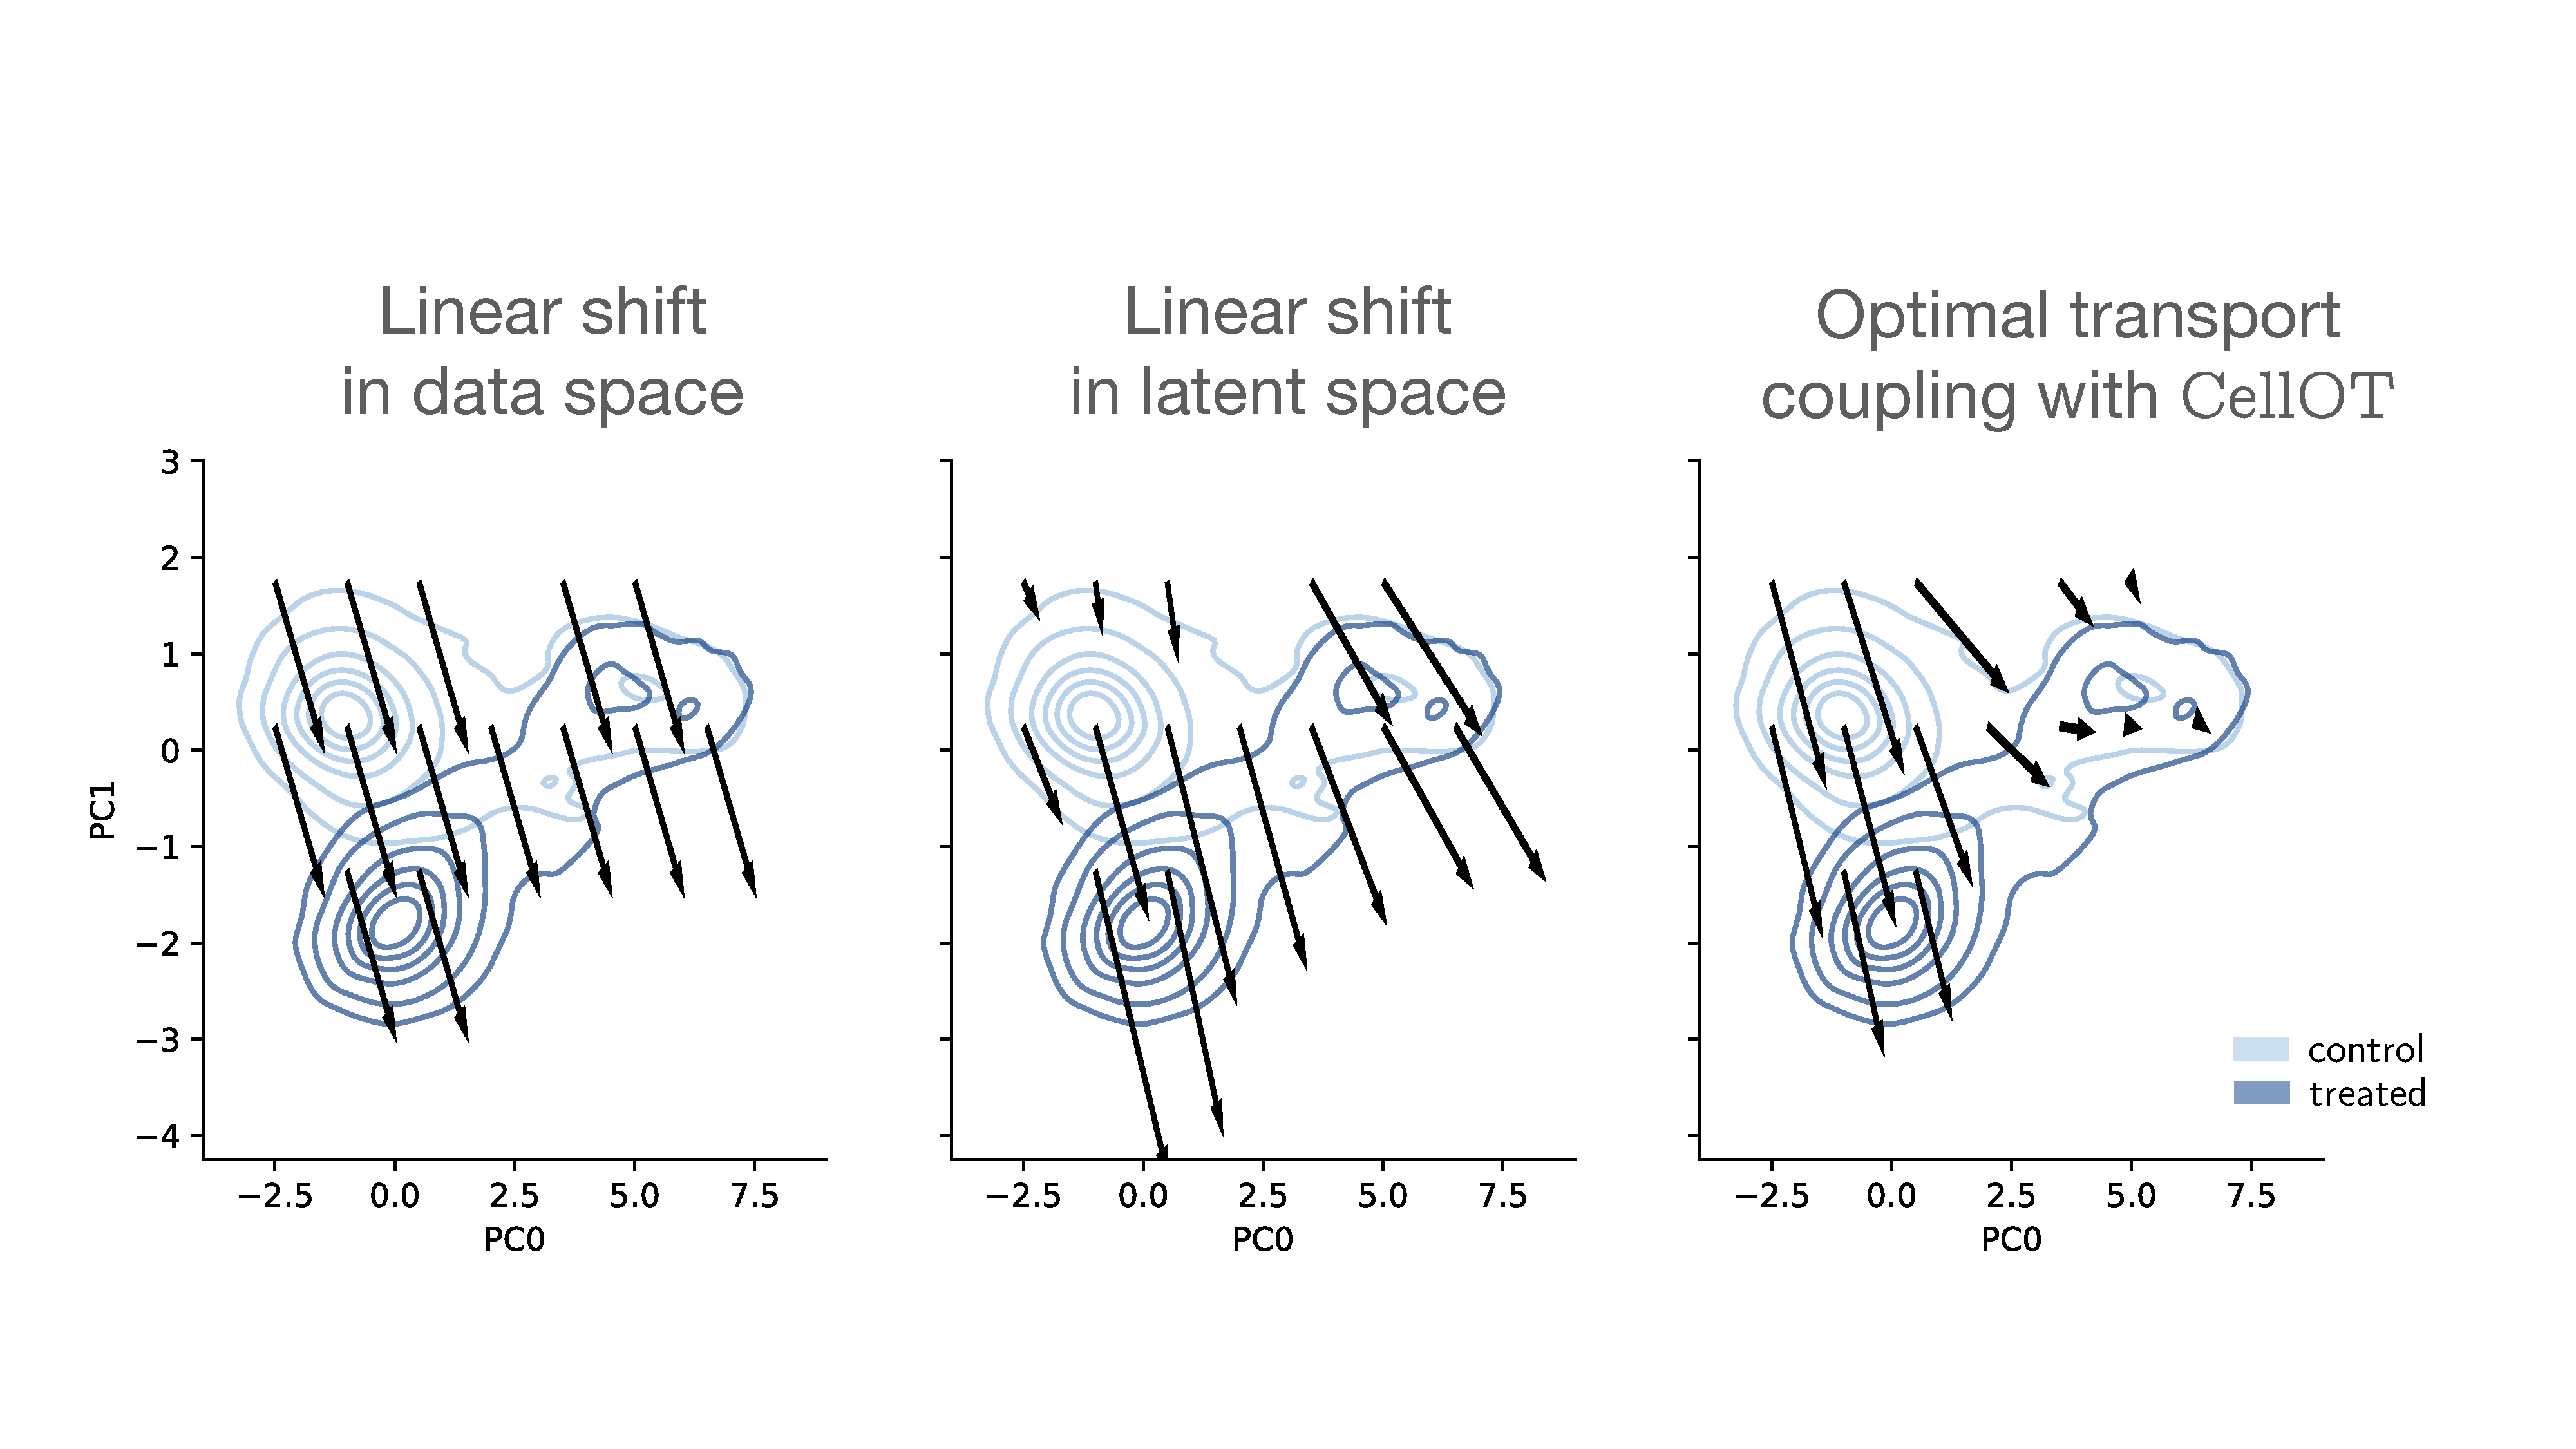
\includegraphics[width=0.95\textwidth]{figures/cellot-methods/arrow-cartoons.pdf}
  \end{center}
  \caption{Approaches to modeling single-cell perturbations. The control (light blue) and treated (dark blue) states are shown as a KDE plot. Arrows depict how each of the three approaches would predict responses at each location in feature space.}
  \label{fig:arrows}
\end{figure}


\subsection{Cell-type approaches}  % TODO: linear shifts in dataspace
Within one sample distinct cell types might exhibit very different responses toward a perturbation. This heterogeneity suggests modeling perturbation effects by first identifying different subpopulations and then predicting the response for each of those subpopulations individually. In the following, we introduce a method built upon that insight, which serves as a baseline in this study.

\paragraph{PopAlign}

\citet{chen2020dissecting} predict gene expression changes that occur in complex single-cell populations by identifying distinct subpopulations within that heterogeneous mixture for both the control $\rho_c$ and treated population $\rho_k$, and comparing as well as aligning those subpopulations in control and treated state through a probabilistic model.
To robustly identify those subpopulations, the data $X = \{ \mathbf{g}_i \}_{i=1}^k$ consisting of $n$-dimensional gene vectors $\mathbf{g}_i = (g_i^1, g_i^2, \dots, g_i^n)$ for each of the $k$ cells is embedded in a lower $m$-dimensional space using orthogonal nonnegative matrix factorization (oNMF) \citep{asteris2015orthogonal}, i.e., $Z = \{ \mathbf{c}_i \}_{i=1}^k$ with $\mathbf{c}_i = (c_i^1, c_i^2, \dots, c_i^m)$. oNMF is known to produce a meaningful set of features as the resulting representation is a superposition of largely disjoint features, here genes, shown to work well for clustering tasks.
This cluster structure then serves as the foundation to identify and represent subpopulations in both the control and subpopulation as $l$ independent Gaussian mixtures, i.e., $P(Z) = \sum_i^l w_i \mathcal{N}(Z; \mu_i, \Sigma_i)$ with weights $w_i$, centroids $\mu_i$, and covariance matrices $\Sigma_i$.
These parameters associated with each Gaussian density $(w_i, \mu_i, \Sigma_i)$ have a natural correspondence to the biological structure and semantics of those cell populations.
Lastly, to understand the perturbation response of each subpopulation, \citet{chen2020dissecting} align subpopulations identified in the control population to those identified in the target population based on a measure of \emph{closeness}, such as Jeffrey's divergence utilized in their work. The resulting statistical alignment allows us to determine the subpopulation-specific perturbation effect through the change in all parameters, i.e.,
\begin{align*}
	\Delta \boldsymbol{\mu}_i &=\left\|\mu_i^{\text {control}}-\mu_j^{\text {treated}}\right\|_2, \\
	\Delta \boldsymbol{\Sigma}_i &=D_{\mathrm{C}}\left(\Sigma_i^{\text {control}}, \Sigma_j^{\text {treated}}\right), \\
	\Delta w_i &=\left|w_i^{\text {control}}-w_j^{\text {treated}}\right|,
\end{align*}
with $D_C$ denoting the Forstner metric. Predictions on unseen control cells can be thus obtained by projecting each cell into the low-dimensional oNMF space, assigning each cell to the corresponding subpopulation, obtaining the corresponding treated state through modeling the perturbation effect via $(\Delta \mu, \Delta \Sigma, \Delta w)$, and lastly, projecting these predicted treated cell states back into the original $n$-dimensional gene space.

\subsection{Mechanistic and other approaches}
Mechanistic models \citep{yuan2021cellbox, frohlich2018efficient} define mathematical models of molecular interactions to model the effect of perturbation.
These methods, however, are restricted to simpler and well-understood systems as they do not capture highly nonlinear perturbation responses of a heterogeneous cell population. Further, these methods are limited in their applicability as they do not scale to genome-wide measurements \citep{snijder2012single, berchtold2018systems, green2016systems}.
Linear models \citep{dixit2016perturb, kamimoto2020celloracle}, on the other hand,  predict changes in cellular gene expression levels using regularized regression methods, where the model predicts a gene's expression level as a linear combination of effects of different perturbations, fitting the regulatory effect of each perturbation on each gene.
Due to assuming only linear relationships of individual genes in response to a perturbation, these methods are similarly  unable to capture complex and inhomogeneous population responses upon perturbation.
\citet{heydari2022iqcell}, on the other hand, predict perturbation responses through inferring the underlying gene regulatory network. Prediction of the perturbed states is achieved through a dynamic simulation of those logical gene networks. Thus, the predicted perturbed states are restricted to only the selected set of genes used to build the corresponding regulatory network.


\subsection{Single-cell perturbation response analysis}
Beyond these tools, a series of methods have been developed to study the nature of perturbation effects on single-cell data. Several works hereby have concentrated on deciphering and disentangling various cellular and genetic patterns within perturbation responses.
\citet{chen2020uncovering}, for example, provide a tool for uncovering different axes of cell variation. A pairwise comparison of identified cell subtypes thereby allows an analysis of patient-to-patient variability.
Similarly, \citet{bhalla2021patient} derive a patient similarity network that identifies patient subgroups by analyzing genetic and molecular landscapes from multi-omics data.
Instead of clustering patients with similar perturbation responses, other tools have tried to dissect variability on the cell level.
For this, \citet{chari2021whole} cluster PCA-based representation of control and perturbed cell populations. Given cell type annotations, they quantify perturbation effects by computing the $\ell_1$ distances between centroids of each cell type cluster.
\citet{skinnider2021cell} construct a classifier-based framework where cell types most responsive to perturbations show a high separability between control and treated cell states within a high-dimensional space. \citet{burkhardt2021quantifying} achieve a similar analysis by introducing a continuous measure based on the relative likelihood estimate of  observing a cell in each experimental condition. Lastly, \citet{petukhov2022case} provide a computational suite to carry out statistical tests that, among others, allows to test variability between different samples and conditions.
Lastly, due to the absence of ground truth when predicting single-cell perturbation responses, various methods have concentrated on simulating single-cell RNA-seq data that capture important properties of experimental data. \citet{cao2021benchmark} provide a comprehensive benchmark study for simulation methods, while at the same time introducing evaluation metrics to measure quantitative and qualitative properties of the RNA-seq data generated by various methods. 
Most importantly, while all those methods contribute to a better understanding of single-cell perturbation responses, they do not allow to predict perturbed states of unseen unperturbed cells, such as those from an incoming patient.



\subsection{Representation learning approaches for heterogeneous models}  % linear shifts in latent space
Current state-of-the-art methods~\citep{Lopez2018scvi, lotfollahi2019scgen, yang2020predicting} aim to learn low-dimensional representations of inputs using autoencoders such that perturbation effects can be applied with simple linear interpolations in representation space. Thus, they predict perturbation responses via linear shifts in a learned low-dimensional latent space. These models are attractive because they are fully parameterized, enabling us to make predictions on unseen cells. By tackling the task of perturbation response predictions via the even more challenging task of learning a meaningful low-dimensional embedding, these methods can be expected to, at best, only perform moderately well. Therefore, we sought to learn a fully parameterized perturbation model that robustly describes the cellular dynamics upon intervention while accounting for underlying variability across samples. More details on both methods are provided in Supplementary Section~\ref{supp:ae_methods}.
% Further, modeling perturbation responses via a matching problem was considered in \citet{suppstark2020scim} for mapping cell populations that are profiled with different profiling technologies.

\subsubsection{Modeling perturbation responses as shifts in latent space} \label{supp:ae_methods}
% \label{sec:related}
Consider a single-cell dataset of a binary perturbation.
Let $\{x_1 \ldots x_n\}$, $x_i \in \mathcal{X}$, drawn from $\rho_c \cup \rho_k$
and let $c(i) \in \{0, 1\}$ indicate the perturbation status of a single cell,
\[
    c(i) = 
\begin{cases}
    0, & \text{if } x_i \sim \rho_c\\
    1, & \text{if } x_i \sim \rho_k.
\end{cases}
\]

\paragraph{scGen}
Given representations $\{z_1 \ldots z_n \}$ of $\{x_1 \ldots x_n\}$, learned by an autoencoder, with encoder $\phi$ and decoder $\psi$,
\textsc{scGen} \citep{lotfollahi2019scgen} predicts a perturbation response using latent space arithmetic.
Let $\bar{z}^{(l)}$ be the mean of representations in condition $l$
\begin{equation*}
    \bar{z}^{(l)} = \frac{1}{|\{i: c(i) = l\}|} \sum{z_i \delta_{c(i)l}},
\end{equation*}
the perturbed state of $x^\prime \sim \rho_c$ is predicted as
\begin{equation*}
    \psi(\phi(x^\prime) - \bar{z}^{(0)} + \bar{z}^{(1)}).
\end{equation*}

\paragraph{\textsc{cAE}}
The conditional autoencoder is based on a popular batch correction technique within the single-cell community, first introduced by~\citep{Lopez2018scvi}.
It introduces condition-specific parameters into the encoder and decoder that attempt to remove and replace information in the data specific to their conditions.
They operate by concatenating one-hot encodings of condition labels (here, perturbation status) to the inputs of the encoder and decoder.
These encodings, in effect, make the bias term in the first layer of the encoder and decoder a learnable parameter specific to each condition. I can thus be considered equivalent to learning a linear shift in the latent space.
Given an encoder $\phi$ and decoder $\psi$, the network is trained to reconstruct cells conditioning on its true label
\begin{align*}
    z_i = \phi( x_i | c(i)), \quad \quad \hat{x}_i = \psi(z_i | c(i)).
\end{align*}
Once trained, the perturbed state of $x^\prime \sim \rho_c$ is predicted as
\begin{align*}
        z_i = \phi( x^\prime | 0), \quad \quad \hat{x}^\prime = \psi(z_i | 1).
\end{align*}

% TODO: major pass over all of this
% OT to dual formulaiton uses general cost, then introduce Euclidiean costs at brenier's
\section{Optimal Transport}
Optimal transport (OT) is a rich branch of mathematics that describe how to manipulate and transform probability distributions.
It plays a pair of roles:
(i) inducing a mathematically well-characterized distance measure between distributions
and (ii) providing a geometry-based approach to realize couplings between two probability distributions.

Let $\mu$ and $\nu$ be probability measures over spaces $\mathcal{X}$ and $\mathcal{Y}$ respectively,
and $T : \mathcal{X} \mapsto \mathcal{Y}$ be a function that moves points across these spaces.
$\mu$ will be some source distribution that will be transformed, under the plan defined by $T$ into the target distribution $\nu$.

\paragraph{Push-forward operator}
As optimal transport describes how to transform probability measures,
it is convenient to introduce notation to help describe these transformations.
While $T$ is a function that maps individual points from $\mathcal{X}$ to $\mathcal{Y}$,
the push-forward operator, $\sharp$, allows $T_\sharp$ to
map a \emph{whole} probability measure on $\mathcal{X}$ to a probability measure on $\mathcal{Y}$.
Intuitively, the push-forward applies the function $T$ to all of the elementary mass particles in the measure $\mu$,
thereby, "pushing" the measure $\mu$ over $\mathcal{X}$ onto some measure on $\mathcal{Y}$.

While the push-forward operator can be defined over arbitrary probability measures \cite{villani2009},
we consider the discrete case here for simplicity.
Given a discrete distribution $\alpha$ over $\mathcal{X}$, $\alpha = \sum_i \mathbf{a}_i \delta_{x_i}$
where $\sum_i \mathbf{a}_i = 1$ and $\delta_a$ is the dirac delta concentrated at some location $x \in \mathcal{X}$,
the push-forward operator is defined as 
\begin{equation}
  \label{eq:def-pushfwd}
  T_\sharp\alpha := \sum_i \mathbf{a}_i \delta_{T(x_i)}
\end{equation}
and $T_\sharp\alpha$ now describes a discrete probability distribution over $\mathcal{Y}$.

\subsection{Monge Maps}
% Let $\mu$ and $\nu$ be two measures in $\mathbb{R}^d$ and a cost function $c: \mathcal{X} \times \mathcal{Y} \mapsto \mathbb{R}$.
The optimal transport problem as formulated by Monge identifies the function
$T^\star$ that transforms $\mu$ into $\nu$, i.e. $T_\sharp \mu = \nu$,
by moving mass as efficeiently as possible according to the cost $c$.
It is defined as
\begin{equation}
  % T^\star = {\arg \inf}_{T : T_\sharp \mu = \nu} \int_{\mathcal{X}} c(x, T(x))d\mu(x)
  T^\star = {\arg \inf}_{T : T_\sharp \mu = \nu} \mathbb{E}_\mu c(x, T(x))
  \label{eq:monge}
\end{equation}

%\paragraph{Monge maps for discrete distributions}
Consider two uniform discrete probability distributions, $\mu$ and $\nu$, of size $n$,
$\mu = \frac{1}{n} \sum_{i=1}^n \delta_{x_i}$
and $\nu = \frac{1}{n} \sum_{j=1}^n \delta_{y_j}$.
In this special case, the Monge problem is an assignment problem: % TODO: cite smth
\begin{equation}
  \min_{\sigma \in \text{Perm}(n)} \frac{1}{n} \sum_{i=1}^{n} \mathbf{C}_{i,\sigma(i)}
\end{equation}
where $\mathbf{C}_{i,j} := c(x_i, y_j)$ is the cost to assign $x_i$ to $y_j$,
that is, $T^\star(x_i) = y_{\sigma(i)}$.
$\mathbf{C}$ can be considered as the weighted adjacency matrix of the bipartite graph that connects elements of $\mu$ to elements of $\nu$.
Here, the optimal transport problem and bipartite matching problem are equivalent.
% TODO: link to bipartite matching in SCIM section

%\paragraph{Limitations}
The Monge formulation in equation \ref{eq:monge} comes with its own set of limitations and challenges.
Firstly, its optimization is a complex non-convex problem.
Furthermore, its reliance on a \emph{deterministic} transport function $T$ restricts the set of problems it can be applied to.
Consider for instance that $\mu$ and $\nu$ are uniform discrete probability measures over $n$ and $m$ items, respectively.
If $n < m$, then there cannot exist a Monge solution as there is no way for a $T$ to assign a source $x_i$ to more than one target $y_j$.
Similarly, solutions for non-uniform discrete measures are not guaranteed to exists,
due to limitations stemming from this determinism.

\subsection{Kantorovich relaxation}  % eqn 2.24 in computational OT
\citeauthor{kantorovich1942} provides a formulation to address these shortcomings with a relaxation to the
Monge problem that allows for non-deterministic transportation by "splitting" mass.
The \citet{kantorovich1942} optimal transport formulation is 
\begin{equation}\label{eq:ot-kantorovich}
W(\mu, \nu)= \inf _{\gamma \in \Gamma(\mu, \nu)} \mathbb{E}_{(X, Y) \sim \gamma}c(x, y)
\end{equation}
where the polytope $\Gamma(\mu, \nu)$ is the set of all joint distributions (or couplings) $\gamma$ between $\mu$ and $\nu$.
The optimal transport plan $\gamma^\star$ that minimizes the Wasserstein distance thus corresponds to the coupling between two probability distributions minimizing the overall transportation cost.
Computing optimal transport distances in \eqref{eq:ot-kantorovich} involves solving a linear program,
and thus their computational cost is prohibitive for large-scale machine learning problems.
Regularizing objective \eqref{eq:ot-kantorovich} with an entropy term results in significantly more efficient optimization
\citep{cuturi2013} and differentiability w.r.t. its inputs, and is commonly used as a loss function in machine learning applications.

% \begin{equation}\label{eq:ot-reg}
% W_{2}^{2, \varepsilon}(\mu, \nu)=\inf _{\gamma \in \Gamma(\mu, \nu)} \int\|x-y\|^{2} d \gamma(x, y) - \varepsilon H(\gamma),
% \end{equation}
% with entropy $H(\gamma) = -\sum_{ij} \gamma_{ij} (\log \gamma_{ij} - 1)$ and parameter $\varepsilon$ controlling the strength of the regularization. $W_{2}^\varepsilon$ is further differentiable w.r.t. its inputs and thus 

\paragraph{Kantorovich Dual}
Problem~\eqref{eq:ot-kantorovich} denotes the primal formulation for the Wasserstein distance. The corresponding dual introduced by \citeauthor{kantorovich1942} in \citeyear{kantorovich1942} is a constrained concave maximization problem defined as
\begin{equation} \label{eq:ot-dual}
    W(\mu, \nu)=\sup _{(f, g) \in \Phi_{c}} \mathbb{E}_{\mu}[f(x)]+\mathbb{E}_{\nu}[g(y)],
\end{equation}
where the set of admissible potentials is $\phi_c := \{(f, g) \in L^{1}(\mu) \times L^{1}(\nu): f(x)+g(y) \leq c(x, y)$, $\forall(x, y) d\mu \otimes d\nu \text{ a.e.}\}$ \citep[Theorem 1.3]{villani2003}.
% TODO: maybe add intuition here

\subsection{Brenier's Theorem}
% TODO: minor describe
A particular interest of optimal transport is the setting $\mathcal{X} = \mathcal{Y} = \mathbb{R}^d$ and $c(x, y) = \frac{1}{2} \| x - y \|^2$.
Thanks to a series of results often attributed to Brenier \cite{knott1984,brenier1991}
some convenient simplifications can be made to the Kantorovich dual formulation \ref{eq:ot-dual}.

These are summarized in \citet[Theorem 2.9]{villani2003} where the dual problem \ref{eq:ot-dual} over the pair of functions $(f, g)$ is simplified to
an optimization over a single $f$ and its convex conjugate, $f^*$, $f^*(y) = \sup_x \left<x,y\right> - f(x)$:
\begin{equation} \label{eq:ot-dual-brenier}
    W(\mu, \nu)= \frac{1}{2}\mathbb{E}\left[\|x\|_{2}^{2}+\|y\|_{2}^{2}\right]-\inf _{f \in \Tilde{\Phi}} \mathbb{E}_{\mu}[f(X)]+\mathbb{E}_{\nu}\left[f^{*}(Y)\right],
\end{equation}
where $\Tilde{\Phi}$ is the set of all convex functions in $L^1(d\mu) \times L^1(d\nu)$ and
$L^{1}(\mu)$ is the set of measurable $f$ such that $\mathbb{E}_\mu f(x) < \infty$.
Furthermore, these results find that the optimal transport plan corresponds to the \emph{gradient} of this convex conjugate, $\gamma^\star = \nabla f^\star$.
\citet[Theorem 2.9]{villani2021} then proves the existence of an optimal pair $(f, f^*)$ of lower semi-continuous proper conjugate convex functions on $\mathbb{R}^n$ minimizing \eqref{eq:ot-dual}.

\subsection{Optimal transport applications in single-cell biology}
Following pioneering work by \citet{schiebinger2019}, numerous problems in single-cell biology have recently been approached using optimal transport.
These problems include mapping cells across perturbations, time points, experimental batches, as well as reconstructing spatial structure from gene expression.
In contrast to previous approaches \citep{schiebinger2019, lavenant2023},
we seek to learn and thus parameterize the optimal transport map $T$ to allow forecasting and predictions on \emph{unseen} cell populations,
i.e., in the out-of-sample setting.
Existing methods addressed proposed neural network-based OT models that directly parameterize $T$ \citep{leygonie2019, yang2019, prasad2022}.
This, however, has been shown to yield an unstable and difficult-to-solve optimization problem~\citep[Table 1]{makkuva2020}.

% TODO: minor rephrase to connect
\section{Neural Optimal Transport}
The computed couplings made by traditional OT approaches rely on observations of the source and target distributions.
This reliance represents a strong limitation in terms of their viability in \emph{prediction} tasks.
For example, in the context of single-cell perturbation prediction,
these approaches would require that some set of perturbed states are always present,
thus are limited in terms of their applications.

Neural OT methods address this limitation by constructing frameworks to parameterize and learn the transport plan $T$ using neural networks.
While the formulation described in Equation $\ref{eq:ot-dual}$ is valid for arbitrary cost functions,
imposing its constraint that the coupling $g(x) + f(y) \leq c(x, y)$ must be enforced everywhere during optimization is generally quite difficult.
A popular approach is to instead build upon the celebrated results by \citet{knott1984} and \citet{brenier1991}
and operate from the formulation described in Equation $\ref{eq:ot-dual-brenier}$.
The optimization scheme within this approach is easier to implement, however, it does require
the adoption of an Euclidean cost function and a framework to parameterize the convex function $f$.
Ultimately, the parameterization of the optimal transport plan $T$ is achieved using the gradient of the convex conjugate of $f$, $\nabla f^*$.

\paragraph{Input Convex Neural Networks}
%\subsection{Convex neural networks}
% Convex neural network architectures are neural networks $f(x; \theta)$ with specific constraints on the architecture and parameters $\theta$, such that the output is a convex function of some elements of the input $x$~\citep{amos2017input}.
Convex spaces such as $\Tilde{\Phi}$ in \eqref{eq:ot-dual-brenier}, can be parameterized utilizing neural networks which are convex w.r.t. to their inputs. One such parameterization approach are input convex neural networks (ICNNs) introduced by \citet{amos2017}.
ICNNs are based on fully-connected feed-forward networks that ensure convexity by placing constraints on their parameters.
An ICNN with parameters $\theta = \{b_i, W^z_i, W^x_i\}$ represents a convex function $f(x; \theta)$ and, for a layer $i = {0 \ldots L-1}$, is defined as
\begin{equation}
    h_{i+1} = \sigma_i(W^x_ix + W^z_i h_i + b_i)  \text { and } f(x; \theta) = h_L,
\end{equation}
where activation functions $\sigma_i$ are convex and non-decreasing, and elements of all $W^z_i$ are constrained to be nonnegative.
Despite these constraints, ICNNs are able to parameterize a rich class of convex functions.
In particular, \citet{chen2020} provide a theoretical analysis that any convex function over a convex domain can be approximated in sup norm by an ICNN.
\citet{huang2021} further extend ICNNs from fully-connected feed-forward neural networks to convolutional neural architectures.

\subsection{Parametrization of the optimal transport map}
% TODO: fix the x and y in this section. Always f(y) and g(x) 
To parameterize the optimal transport plan, we follow the approach taken by \citeauthor{makkuva2020} which 
in turn builds off of a previous approach described by \citet{taghvaei2019}.
This approach considers solving \eqref{eq:ot-dual-brenier} by parameterizing $f$ with an ICNN and directly solving, at each update step, an optimization problem to compute the convex conjugate $f^*$.
As these updates are costly, \citet{makkuva2020} relax the strict dependency between $f$ and $f^*$
through an approximation of $f^*$ with another ICNN $g$.
This results in a min-max optimization problem over a pair of competing convex neural networks:
\begin{equation} \label{eq:ot-makkuva}
  W_{2}^2(\mu, \nu)=\sup _{\substack{f \in \Tilde{\Phi}}} \inf _{g \in \Tilde{\Phi}}  \underbrace{\frac{1}{2}\mathbb{E}\left[\|x\|_{2}^{2}+\|y\|_{2}^{2}\right]}_{\mathcal{C}_{\mu, \nu}} - \underbrace{\mathbb{E}_{\mu}[f(x)]-\mathbb{E}_{\nu}[\langle y, \nabla g(y)\rangle-f(\nabla g(y))]}_{\mathcal{V}_{\mu, \nu}(f, g)}.
\end{equation}
Where we have utilized the fact that
\begin{equation}
  \mathbb{E}_\mu \left[f^*(x)\right] = \max_{g \in \Tilde{\phi}} \mathbb{E}_\mu \left[ \left<x, \nabla g(x)\right> - f(\nabla g(x))\right]
  \label{eq:ot-makkuva-hint}
\end{equation}
and 
$\left<x, \nabla g(x)\right> - f(\nabla g(x)) \leq f^*(x)$ for all functions $g$ with equality when $g=f^*$.
Finally, the parameterization of the optimal transport plan $T^\star$ is achieved by solving the min-max problem:
\begin{equation}
  (g^\star_\theta, f^\star_\phi) \leftarrow \arg \max_\phi \min_\theta \mathcal{C}_{\mu,\nu} - \mathcal{V}_{\mu, \nu}(g_\theta, f_\phi)
  \label{eq:ot-makkuva-optim}
\end{equation}
where $T^\star = \nabla g^\star_\theta$ and $\theta$ and $\phi$ are the parameters the ICNNs.

% In order to learn the resulting optimal transport, i.e., the solution of the minimization problem in \eqref{eq:ot-makkuva}, \citetmain{makkuva2020optimal} parameterize both dual variables $f$ and $g$ using ICNNs \citep{amos2017input} and yields a transport plan with the graident of $g$.
% The resulting approximate Wasserstein distance is thus defined as
% \begin{equation} \label{eq:cellot-optim}
%     \hat{W}_2^2(\mu, \nu) = \sup _{\phi} \inf_{\theta}  \mathcal{C}_{\mu, \nu} - \mathcal{V}_{\mu, \nu}(f_{\phi}, g_{\theta}),
% \end{equation}
% where $\phi$ and $\theta$ are the parameters of the ICNNs underlying $f$ and $g$ respectively.


\paragraph{Other approaches}
Other appraoches, for example taken by \citet{huang2021} introduce a novel, OT-inspired parameterization of normalizing flows utilizing ICNNs.
\citet{korotin2020} provide a detailed comparison of the current state of neural optimal transport solvers.
Furthermore, convex neural architectures have been utilized to parameterize Wasserstein gradient flows
\citep{bunne2022, alvarez-melis2022, mokrov2021} as well as barycenters \citep{fan2021}.


\section{Learning and predicting single-cell responses with \textsc{CellOT}}
% TODO: minor: connect flow

% Small molecule drugs can have profound effects on the cellular phenotype by, for instance, altering signaling cascades.
% Most of these effects depend on the context in which the perturbation occurs.
% Given the heterogeneity among single cells in cell populations and tissues, predicting cellular responses requires understanding the rules by which context shapes genome activity and its response to drugs.
% High-dimensional single-cell data measured via single-cell genomics or multiplexed imaging technologies can provide this contextual information but only return  unpaired or unaligned observations of cell populations.
% Here, \textsc{CellOT} allows us to utilize such unpaired data and enables learning cell state transitions upon perturbation.

In formal terms, we denote the unperturbed control population by $\mu$ consisting of $n$ cells $x_i$ for $i = 1, \dots, n$.
Upon perturbation $k$, the multivariate state of each cell $x_i$ of the unperturbed population changes, which we observe as the perturbed population $\nu$ (\textbf{Fig \ref{fig:fig_1}a}).
To understand the mode of action and effect of perturbations, we seek to learn the transition and alignment between populations $\mu$ and $\nu$ via parameterizing a map $T$ (see \textbf{Fig \ref{fig:fig_1}a-b}), which explains the transition of each cell from the unperturbed cell population $\mu$ into their perturbed state $\nu$ upon treatment $k$.
Despite originating from  different observations, map $T$ determines for each cell $x_i$ the most likely corresponding cell $T(x_i)$ in the perturbed population (\textbf{Fig \ref{fig:fig_1}c}).
Finding this map then not only allows us to model single-cell trajectories upon perturbation but also to predict the perturbed state of previously unseen control cells.
As a result, we can forecast the outcome of a perturbation $k$  by applying the learned map $T$ to a new unperturbed population $\rho^\prime_c$ (\textbf{Fig \ref{fig:fig_1}d}).

The optimal map $T$ aligning the control and perturbed population, which we seek to find, should best describe the incremental changes in the multivariate profile of each cell after applying a perturbation $k$.
Using optimal transportation theory \cite{villani2021topics, santambrogio2015optimal} to recover these maps and unveil single-cell reprogramming trajectories has been proposed as a strong modeling hypothesis in the domain of single-cell biology \cite{schiebinger2019optimal, cang2020inferring, demetci2020gromov, huizing2021optimal, lavenant2021towards, zhang2021optimal}.
Optimal transport problems return the alignment between distributions $\mu$ and $\nu$ corresponding to the minimal overall cost between aligned molecular profiles, thus determining the most likely state of each cell upon perturbation (Fig \ref{fig:fig_1}c).
$T$ is learned such that its image corresponds to $\nu$ and mass is moved from $\mu$ into $\nu$ according to a principle of minimal effort.
% Utilizing recent advancements in neural optimal transport theory, \textsc{CellOT} considers the dual form of the transport problem and parameterizes a pair of convex potentials with neural networks.
$T$ is recovered as the gradient of one of these potentials.
As directly parameterizing the optimal transport map $T$ \cite{korotin2019wasserstein, yang2018scalable, prasad2020optimal} is unstable \citep[Table 1]{makkuva2020optimal}, we parameterize the convex potentials of the dual optimal transport problem $f$ and $g$ by convex neural networks \cite{amos2017input} and recover the optimal map $T$ using the gradient of a convex function $g_k$, i.e., $\nabla g_k$ \cite{makkuva2020optimal}.
Supplementary Section \ref{supp:related_work} provides a more detailed review of optimal transport methods proposed for single-cell biology problems and how our approach deviates from previous methods.

To put \textsc{CellOT}'s performance in perspective, we benchmark it against current state-of-the-art autoencoder-based methods cite{lotfollahi2019scgen, Lopez2018scvi},
which attempt to add perturbation effects through the manipulation of a learned latent representation (review in Supplementary Section \ref{supp:related_work}).
To further test the hypothesis of the optimal transport modeling prior, we compare the learned OT map $\nabla g_k$ for each perturbation $k$ with naive non-OT-based alignments.


% TODO: minor: insert cellot figure 1 here

% \begin{itemize}
%   \item lack of ground truth complicates evaluation
%   \item metrics to measure alignment of distributions
%     \begin{itemize}
%       \item mean-based metrics
%       \item MMD (describe in supplment ?)
%     \end{itemize}
%   \item analyses to verify responses
% \end{itemize}

\subsection{Evaluation strategies}
% TODO: minor rephrase
Since we lack access to the ground truth set of control and treatment observations on the single-cell level,
we analyze the effectiveness of \textsc{CellOT} using evaluations that operate on the level of the distribution of real and predicted perturbation states.
Three metrics are considered, i.e., MMD, $\ell_2$ feature means, and the average correlation of the feature means.

$\ell_2$ feature means refers to the $\ell_2$-distance between means of the observed and predicted distributions. Similarly, $r$ feature means refers to the correlation of the means of the observed and predicted distributions.
However, metrics based only on feature means can be insensitive in settings where heterogeneity is not captured. Consider, for example, a target distribution with multiple modes. These metrics will favorably evaluate a uni-modal predicted distribution that simply models the mean of this multi-modal distribution. To this end, we include a distributional distance sensitive to this type of behavior by measuring differences in the properties of higher moments, i.e., the maximum mean discrepancy.
% Let $r_c$ be a set of observed untreated cells, $r_k$ be a set of observed cells treated with perturbation $k$, and $\hat{r}_k$ be the set of predictions made on $r_c$. The drug signature of perturbation is defined as:
% \begin{equation*}
%     DS(r_k, r_c) = \frac{1}{|r_k|}\sum_{x_i \in r_k}{x_i} - \frac{1}{|r_c|}\sum_{y_i \in r_c}{y_i}
% \end{equation*}
% We report the $\ell_2$ distance between the observed signature $DS(r_k, r_c)$ and the predicted signature $DS(\hat{r}_k, r_c)$, which is a function of the difference in the means between the observed and predicted distributions.

MMD refers to the kernel maximum mean discrepancy \citep{gretton2012kernel}, a metric to measure distances between distributions.
Given two random variables x and y with distributions p and q, and a kernel function $\phi$, \citet{gretton2012kernel} define the squared MMD as
\begin{equation*}
    \text{MMD}(p, q; \phi) = \mathbb{E}_{x,x^\prime}[\phi(x, x^\prime)] + \mathbb{E}_{y,y^\prime}[\phi(y, y^\prime)] - 2\mathbb{E}_{x,y}[\phi(x, y)].
\end{equation*}
We report an unbiased estimate of $\text{MMD}(r_k, \hat{r}_k)$ where the expectations are evaluated by averages over the cells in each set. The RBF kernel is employed, and as is usually done, reports the MMD as an average over several length scales, i.e., \texttt{np.logspace(1, -3)}.


\section{Applications of \textsc{CellOT}}
\subsection{Datasets and Tasks}

We apply \textsc{CellOT} to learn treatment responses and development processes in two modalities, 4i \cite{gut2018} and scRNAseq.

\paragraph{4i cell lines}
4i profiles of a mixture of two melanoma cell lines treated with cancer treatments and a control.
The data is released as part of the CellOT paper \cite{bunne2023}.
In total, there are 35 treatments including standard-of-care drugs and combinations.
%with a median 2522 cells per treatment (std=290), plus a control treatment.
As part of the 4i profiling, 48 features are reported, including the intensity of 14 protein markers reported both within and outside the nucleus for a total of 26 intensity features.
The remaining 22 features report extracted morphology features such as the area, nuclei, convexity, etc of the cell and nucleus each.
The task is to learn (i.i.d.) the cell line responses to each treatment.

\paragraph{sciplex3}
scRNAseq profiles of cell lines treated with cancer therapies and a control \cite{srivatsan2020}.
A mixture of three melanoma cell lines, A549 (lung adenocarcinoma), K562 (chronic myelogenous leukemia), and MCF7 (mammary adenocarcinoma), are exposed to a screen of 188 different compounds.
Here we take a subset of 9 cancer treatments for simplicity.
%, with a median 4141 cells per treatment (std=531).
The task is learn (i.i.d.) the cell line responses to each treatment.

\paragraph{lupus samples}
scRNAseq profiles of a small cohort of 8 lupus samples treated with Interferon-$\beta$ (IFN-$\beta$) \cite{need} and a control.
IFN-$\beta$ is known to have a heterogeneous effect within immune cells \cite{stark1998,mostafavi2016}.
The task is to generalize (o.o.s.) the patient IFN-$\beta$ response across samples.
This task is considered out-of-sample since the samples were processed as a single batch.

\paragraph{statefate stem cell development}
scRNAseq profiles of a stem cell population at different stages of development \cite{weinreb2020}.
Stem cells are able to develop into specialized cell types.
Potency refers to the capacity of a stem cell to give rise to different cell lineages.
Here, two classes stem cells of higher and lower potency are allowed to develop over the course of six days, and are profiled every two days.
The task is to generalize (o.o.d.) the development trajectory of the population of higher potency to the population of lower potency.

\paragraph{Cross species LPS}
scRNAseq profiles of control and lipopolysaccharide (LPS) stimulated cells across four different species.
LPS induces an immune response and 
the task is to generalize (o.o.d.) this response to held out species.

\subsection{CellOT outperforms state-of-the-art methods at learning responses}

\begin{figure}
  \begin{center}
    \includegraphics[width=0.95\textwidth]{figures/cellot-methods/Bunne_Main_Fig2.pdf}
  \end{center}
  \caption{}\label{fig:cellot-main-marginals}
\end{figure}

% TODO: decide what to do about supplemental marginals
We apply \textsc{CellOT} to predict the responses of cell populations to cancer treatments using a proteomic dataset consisting of two melanoma cell lines (M130219 and M130429) \cite{raaijmakers2015new}, profiled by 4i \cite{gut2018multiplexed}, and a scRNAseq dataset \cite{srivatsan2020massively}, which contain 34 and 9 different treatments, respectively.
We benchmarked \textsc{CellOT} against two autoencoder-based tools, \textsc{scGen} \cite{lotfollahi2019scgen} and \textsc{cAE} \cite{Lopez2018scvi}, as well as \textsc{PopAlign} \cite{chen2020dissecting}, a method based on aligning subpopulations of the control and treated space approximated through a mixture of Gaussian densities.
Due to the high dimensional nature of scRNA-seq data, we apply $\textsc{CellOT}$ on latent representations learned by an autoencoder.
The marginal distributions for observed and predicted cell populations for two 4i treatments and two scRNAseq treatments are shown in figure \ref{fig:cellot-main-marginals}a, d.
Two features are selected for each perturbation and the complete set of marginals is shown in \textbf{\ref{supp_fig:4i_all_marginals_imatinib}-4}.
While the autoencoder baselines tend to capture the mean of the treated cell population, they are less successful in matching all heterogeneous states of the perturbed population, i.e., higher moments of the perturbed population.
Thus, these models tend to learn over-simplified perturbation effects and are insufficient when aiming to understand heterogeneous rather than average cellular behaviors.
\textsc{CellOT}, on the other hand, is able to capture these higher moments, yielding accurate and nuanced predictions.

This can be further quantified % differences between the distributions of observed and predicted treated cell populations, we determine 
through distributional metrics such as the maximum mean discrepancy (MMD) \cite{gretton2012kernel}.
Low values of MMD imply that all moments of two distributions are matched, and thus the entire distribution of perturbed cells is captured in fine detail, beyond the population average (see Online Methods for details).
The MMDs between the predicted and observed populations for the selected perturbations are shown in figure \ref{fig:cellot-main-marginals}b, e.
For scRNA-seq data, MMD evaluations are computed using the top 50 marker genes. An analysis on the influence of the number of chosen marker genes can be found in \ref{supp_fig:sciplex_num_markers}.
In addition to the autoencoder baselines, we include the trivial \emph{identity} baseline that predicts treatment effects simply by returning the untreated states,
as well as a theoretical lower bound, \emph{observed}, comprising a different set of observed perturbed cells, thus only varying from the true predictions up to experimental noise.
We find that \textsc{CellOT} can approach the lower bound (\emph{observed} setting), while the baseline methods often do not improve much over the \emph{identity} setting.

% TODO: decide what to do about supplemental metrics
Different evaluation metrics across all 35 4i therapies and 6 scRNAseq therapies are summarized in \ref{supp_fig:4i_all_results} and \ref{supp_fig:sciplex_all_results}.
Besides MMD, we additionally include the $\ell_2$(DS) metric that measures the distance between the observed and predicted \emph{mean} drug effect, where these drug signatures are computed as the difference in means between the treated and untreated cell populations.
%Lastly, we compare the overall mean correlation coefficient $r^2$ between the predicted and observed data on all features (see Online Methods).
$\textsc{CellOT}$ outperforms the baselines in both metrics across all treatments, typically by one order of magnitude.
We attribute the strong performance of \textsc{CellOT} to its ability to learn a transport function that considers explicitly the data geometries of cell populations through the theory of optimal transport.
This hypothesis is supported by the observation that the inter-feature correlation structure remains largely conserved between treated and untreated populations, thus depicting a setting where optimal transport approaches excel. For more information, see \ref{supp_fig:data_correlation}.
\ref{supp_fig:4i_vector_fields} visualizes the learned maps, % projected onto the first two principal components, 
further demonstrating \textsc{CellOT}'s ability to model fine-grained responses. % While overall matching the average perturbation effect, it captures the heterogeneity of the treatment response on the single-cell level.

Finally, we compute UMAP projections \cite{umap} on a joint set of predicted and observed perturbed cells utilizing the full feature space, shown in figure \ref{fig:cellot-main-marginals}c, f.
We observe that the perturbed cell states inferred by \textsc{CellOT} are well integrated with the observed perturbed cells. Again, both baselines do not recover the perturbed distribution in its entirety % (via higher order moments)
and thus the perturbed state of different subpopulations is not captured consistently.


\subsection{CellOT captures cell-to-cell variability in drug responses}
Capturing distinct perturbation responses of different cell types within the same sample remains a challenging computational task. To reduce the task's complexity, prediction algorithms can be guided by predefined cell type labels both in the perturbed and unperturbed states \cite{chen2020dissecting} or set to approximate the mean drug response \cite{lotfollahi2019scgen}.  These simplifications come at a cost: the reliance on a priori knowledge about present and relevant cell types, the assumption that cell types are characterized by the same features before and after a perturbation and that the drug response is uniform within a cell type.
In the worst case, these limitations risk masking true and important drug response heterogeneity  and thus hamper the discovery of novel cell type or cell state-specific perturbation responses (see further comparisons in \ref{supp_fig:comparison_cellot_average}).
\textsc{CellOT} is free of these limitations and enables scientists to query the predicted single-cell responses at the granularity best suited to answer their biological questions.
As a proof of concept, we co-cultured the aforementioned patient-derived melanoma cell lines (see Online Methods) at equal ratios and performed a boutique drug screen, during which we exposed cells 8h to a panel of 34 drugs and measured the single-cell drug responses with the 4i technology. 


\begin{figure}
  \begin{center}
    \includegraphics[width=0.95\textwidth]{figures/cellot-methods/Bunne_Main_Fig3.pdf}
  \end{center}
  \caption{}\label{fig:cellot-main-4i-analysis}
\end{figure}
% TODO: write caption

Using \textsc{CellOT}, 
we predict the perturbed cell states of a shared set of control (DMSO-treated) cells (figure \ref{fig:cellot-main-4i-analysis}a) for each drug.
Previous work \cite{kramer2019cellular} shows that phosphorylation levels of signaling kinases upon drug treatments are tightly linked to the cellular state. 
To assess whether this relationship was retained in predicted compared to observed perturbed cells, we analyzed the phosphorylation levels of extracellular signal-regulated kinases (pERK) using the transport maps learned by \textsc{CellOT} on each drug.
Using 750 predicted and 750 observed perturbed cells, we computed UMAP projections joint-wise from all features except pERK.
figure \ref{fig:cellot-main-4i-analysis}b shows the predicted and observed population individually annotated with the respective pERK levels of each cell.
We find the spatial organization of the two projections to look almost identical and that pERK levels had a highly comparable distribution across the cells of either class and all drug treatments (further analysis in \ref{supp_fig:4i_analysis_extended}a, b.

\subsection{CellOT disentangles subpopulation-specific drug effects}
\textsc{CellOT} allows us to 
isolate the mode of action of each drug by computing the difference between predicted perturbed cells and untreated control cells. % , i.e., the \emph{cost} of the optimal transport.
A UMAP embedding of all cells color-coded by the treatment distinctly separates different treatments (figure \ref{fig:cellot-main-4i-analysis}c and \ref{supp_fig:4i_analysis_extended}e), all of which \textsc{CellOT} is able to faithfully learn (\ref{supp_fig:4i_all_results}).
Such distinct treatment embeddings are not present when accounting only for an average perturbation effect (\ref{supp_fig:4i_analysis_extended}d), indicating the importance of capturing the cellular heterogeneity of drug responses.

Using Leiden clustering on the full feature set, we grouped unperturbed control cells in 12 cellular states (figure \ref{fig:cellot-main-4i-analysis}d, \ref{supp_fig:4i_analysis_extended}g.
Cellular states 1, 5, 6, 9, and 12 show high levels of MelA and no SOX9 and thus correspond to the melanocytic cell line M130429, whereas the SOX9\textsuperscript{+} and MelA\textsuperscript{-} states 2, 3, 4, 7, 8, 10, and 11 represent the mesenchymal cell line M130219 (see Online Methods). Overall, we find that M130429 cells have higher phosphorylation levels of the measured signaling kinases compared to M130219;
% The cluster structure derived from the control cells is further persistent in the perturbed states. 
a stereotypical spatial organization of cellular states is retained for the majority of the drugs,  and cell states belonging to the same cell line cluster together (\ref{supp_fig:4i_analysis_extended}f). 

Computing the difference between the control and treated state of each drug, i.e., the optimal
transport cost, allows us to further characterize a drug's severity. 
Apoptosis inducers (e.g., Staurosporine), proteasome inhibitors (e.g., Ixazomig and Carfilzomib or the combination treatment Carfilzomib + Pomalidomide + Dexamethasone), microtubule-stabilizing agents (e.g., Paclitaxel), c-Met inhibitors (e.g., Crizotinib), and ATP competitors for multiple tyrosine kinases such as c-KIT, and Bcr-Abl (i.e., Dasatinib) show high transport costs and thus substantial feature changes in all cellular states (figure \ref{fig:cellot-main-4i-analysis}e).
Other drugs demonstrate less severe effects in the observed 8h incubation period. 
We find all perturbations to increase levels of cleaved Caspase 3, an apoptosis marker, in various cellular states and in both cell lines (\ref{supp_fig:4i_analysis_extended}k),
with the exception of Dasatinib, which specifically induced cell death in cellular states 5, 6, 9, and 19 associated to M130429 (figure \ref{fig:cellot-main-4i-analysis}f).


Previous work by \citet{smith2016inhibiting} reports that M130429 cells reduce metabolic activity % (a proxy of cell viability)
upon treatment with inhibitors of MEK (MEKi) and RAF (RAFi), while M130219 cells are resistant to these inhibitors.
When comparing the responses of the two cell lines to Trametinib (MEKi) and MLN2480 (panRAFi) in the MEK and PI3K pathway using pERK and pAKT as the respective readouts, we find that MEKi-sensitive M130429 cells down-regulate pAKT and pERK, whereas the MEKi-resistant M130219 cells only down-regulate pERK.
Consistently, we also find that treatment with MLN2480 results in a similar differential drug response (\ref{supp_fig:4i_analysis_extended}i).
This suggests that \textit{decoupling} of the MEK and PI3K pathways may confer resistance to MEK and Raf inhibitors and constitute an adaptation to the escape of cancer therapy \cite{kun2021mek}.
We find further supporting evidence of pathway crosstalk alteration when we analyze pAKT and pERK levels upon treatment with a cocktail of Trametinib (MEKi) and Dabrafenib (BRAFi). 

In response to two drugs impinging on the MEK pathway, we observe pERK to be reduced in both cell lines but increased pAKT levels in the MEKi-resistant cell line M130219 (which resistance was acquired during pre-exposing a patient to MEKi) (figure \ref{fig:cellot-main-4i-analysis}f).
This finding points towards a compensatory feedback mechanism acquired by M130219 during MEKi treatment by which inhibition of the MEK pathway (quantified as a reduction of pERK) would stimulate signaling through the PI3K pathway, possibly through activation of an upstream receptor kinase \cite{caunt2015mek1}. 
Our results on two co-cultured primary melanoma cell lines treated with various anti-cancer drugs show that \textsc{CellOT} can accurately capture phenotypic heterogeneity in unperturbed cell populations and predict diverse drug responses by incorporating the underlying cell-to-cell variability without predefined cell line labels. 

\subsection{CellOT accurately infers cellular responses in unseen patients}

\begin{figure}
  \begin{center}
    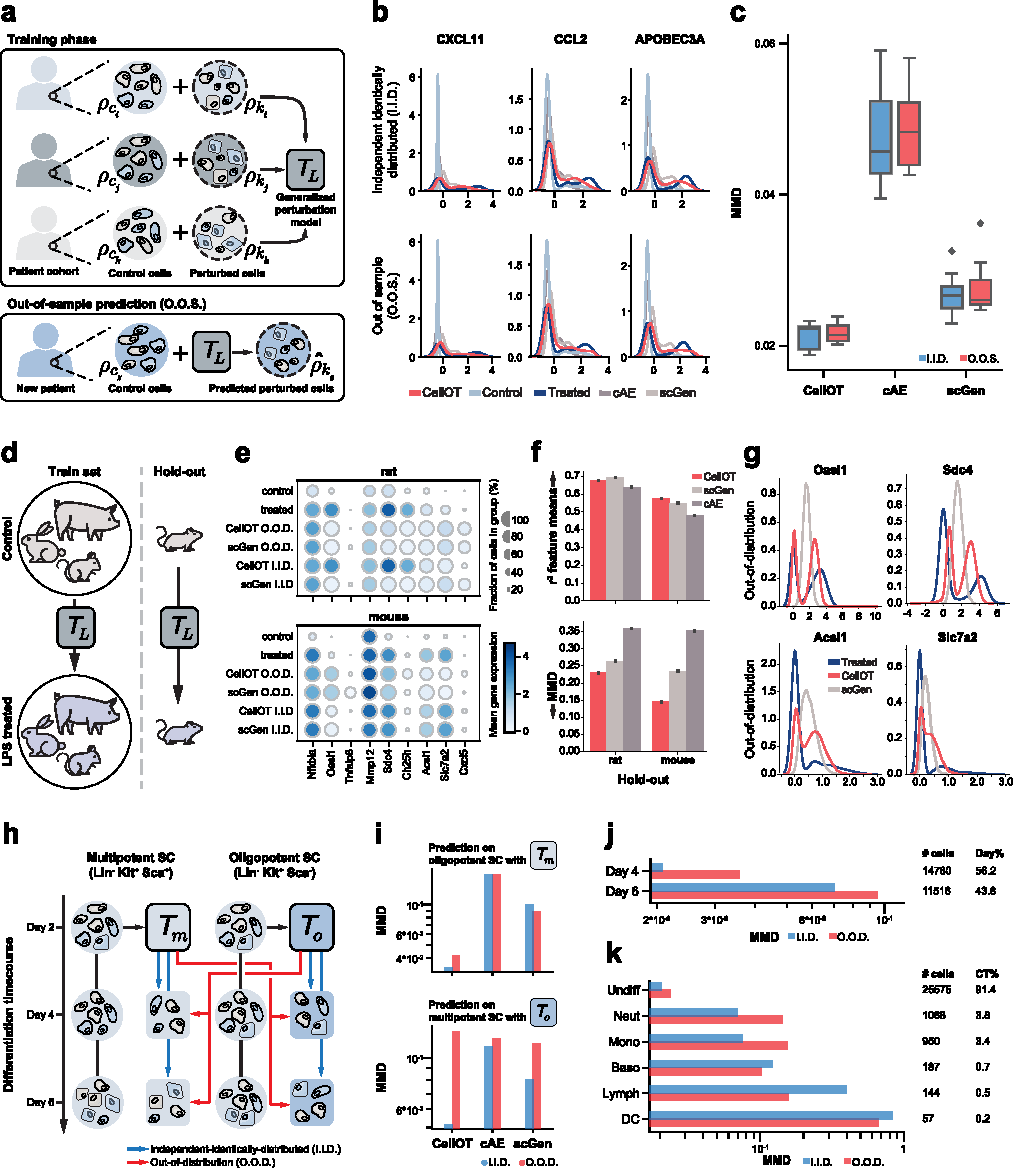
\includegraphics[width=0.95\textwidth]{figures/cellot-methods/Bunne_Main_Fig4.pdf}
  \end{center}
  \caption{}\label{fig:cellot-main-ood}
\end{figure}
% TODO: write caption


The maps between molecular states before and after treatments learned by \textsc{CellOT} contribute to a better understanding of the differences between cells that respond to certain drugs and cells that do not respond. This is crucial for inferring an incoming patient's response to drugs and settings with high cell-to-cell variability.
To make predictions on unseen patients, however, we need to demonstrate that the learned maps $T$ model perturbation responses across different patients coherently and robustly, while still predicting personalized treatment outcomes for each patient instead of mere population averages.
To test the generalization capacity of \textsc{CellOT} in such an out-of-sample scenario, we use a peripheral blood mononuclear cells (PBMC) droplet scRNA-seq dataset. \citet{kang2018multiplexed} characterize the cell type specificity and inter-individual variability of the response of eight lupus patients to interferon beta (IFN-$\beta$), a potent cytokine that induces genome-scale changes in immune cell transcriptional profiles.
In the following, we compare the performance of \textsc{CellOT} and other baselines in an independent-and-identically-distributed (i.i.d.) setting, where models see cells from all patients, as well as in the out-of-sample (o.o.s.) setting, where models do not see cells from a specific holdout patient (see figure \ref{fig:cellot-main-ood}a).

As in the previous analysis, we evaluate how accurately \textsc{CellOT} captures the change in the overall expression of different marker genes from control to IFN-$\beta$-treated cells and thus how well the predicted gene expression marginals are aligned with the treated population (figure \ref{fig:cellot-main-ood}b). Here, we consider the genes \textit{CXCL11}, \textit{CCL2}, and \textit{APOBEC3A},
since they are connected with autoimmune diseases, including systemic lupus erythematosus \cite{hedrich2011epigenetic, perez2021sustained}
and thus potential therapeutic targets
in the management of patients with lupus and, likely, other interferonopathies \cite{mathian2015targeting,rani1996characterization,hedrich2011epigenetic,mathian2015targeting,perez2021sustained,flier2001differential}.
% CXCL11 and CCL2 are both chemokines
% induced by IFN-$\beta$ \cite{need} and have been shown to play a very prominent and often interchangeable role in the mobilization of T cells during a variety of pathological conditions, including cancer, infection, and inflammation, making them potential therapeutic targets \cite{need}.
% Similarly, the cytidine deaminase APOBEC3 contributes epigenetically to autoimmune diseases such as systemic lupus erythematosus \cite{need} and is a potential subject in therapies targeting interferons and specifically A3 enzymes in the management of patients with lupus and probably other interferonopathies \cite{need}.
These selected genes show a large change in expression from the control to the perturbed population, partially exhibiting a bimodal gene expression profile upon perturbation. In contrast to \textsc{CellOT}, the baselines do not accurately predict these large transcriptomic shifts of these genes.
An extended analysis of additional genes strongly affected by the IFN-$\beta$ treatment can be found in the \textbf{\ref{supp_fig:lupus_all_marginals_iid}} and \textbf{\ref{supp_fig:lupus_all_marginals_ood}}.

All models, including \textsc{CellOT}, show little performance drop when modeling the treatment outcome on a new patient using the generalized perturbation model $T_L$ trained on the patient cohort and using the control cells $\rho_{c_z}$ of the unseen patient as input.
This becomes evident when comparing the predicted population $\hat{\rho}_{k_z}$ with observations $\rho_{k_z}$ using the MMD metric. figure \ref{fig:cellot-main-ood}c displays summary results in which each individual patient was considered for the holdout set.
Further evaluation metrics, including the $\ell_2(\text{DS})$ score, can be found in \ref{supp_fig:lupus_iid_ood_l2ds}.
\textsc{CellOT} outperforms previous baselines both in the i.i.d.~and in the o.o.s.~setting, while further showing a smaller performance drop when generalizing to the unseen patient.
For more results, see \ref{supp_fig:lupus_umaps_all}.
These results suggest that the learned optimal transport maps correctly model the shift in the structures of the cellular subpopulation present in all patients, thus robustly performing out-of-sample.
We repeat the same evaluation for a glioblastoma cohort consisting of seven patients \cite{zhao2021deconvolution}.
However, generalization within this setting proved to be difficult for \textsc{CellOT} and all baselines, due to the small size of the cohort and high degree of variance within the responses of each individual. 
% We have identified under which conditions generalization to unseen patients is feasible. 
For a complete analysis, see \ref{supp_fig:gbm_patients_iid_ood}.

\subsection{CellOT reconstructs innate immune responses across species}

The innate immune response is a cell-intrinsic defense program showing high levels of heterogeneity among responding cells -- and thus an ideal task for evaluating \textsc{CellOT}'s capabilities.
We rely our analysis on the dataset collected by \citet{hagai2018gene}, which studies the evolution of innate immunity programs of mononuclear phagocytes within different species, including pigs, rabbits, mice, and rats.
For this, these primary bone marrow-derived cells are stimulated using lipopolysaccharide (LPS).
In the following, we test how well \textsc{CellOT} and the baselines reconstruct innate immune responses within species that are not encountered during training.
We refer to the generalization task as out-of-distribution (o.o.d.), since unlike the o.o.s.~setting, we expect different species to have very distinct responses (see figure \ref{fig:cellot-main-ood}d).
The holdout set thereby consists of cells derived from either rat or mouse. See \ref{supp_fig:crossspecies_ood_analysis}a,b for an analysis of cross-species similarity and the reasoning behind selecting the holdout set.

Indeed, \textsc{CellOT} accurately reconstructs the innate immune response in both mouse and rat in the i.i.d. and o.o.d. setting.
This not only becomes evident through capturing more precisely the mean expression level of marker genes that show high differential expression levels upon addition of LPS, e.g., \textit{Nfkb1} (NF-$\kappa$B), \textit{Oasl1} (Oasl1), \textit{Mmp12}, and \textit{Cxcl5} (see figure \ref{fig:cellot-main-ood}e and \ref{supp_fig:crossspecies_ood_analysis}c-d), but also through the average correlation coefficient $r^2$ computed between o.o.d. predictions and holdout observations across all genes (see figure \ref{fig:cellot-main-ood}f).
In particular, \textsc{CellOT} outperforms the baselines when analyzing how well each method captures the heterogeneity of innate immune responses in different species, as demonstrated by low levels of MMD (see figure \ref{fig:cellot-main-ood}f).
Most impressively, our method shows a strong alignment or gene expression marginals of aforementioned marker genes that show complicated bimodal expression profiles upon perturbation (see figure \ref{fig:cellot-main-ood}g).

% \subsection*{CellOT generalizes perturbation responses out-of-distribution from multipotent populations to cells of lower potency}
\subsection{CellOT extends differentiation results to cells of lower potency}

During developmental processes, stem and progenitor cells progress through a hierarchy of fate decisions, marked by a continuous differentiation of cells that refine their identity until reaching a functional end state.
% Modern high-throughput methods allow us to monitor these successive changes in gene expression profiles by observing multiple snapshots over time. To ultimately associate molecular differences among progenitor cells with their capacity to generate mature cell types and get a better understanding of biological differentiation or reprogramming mechanisms, we are required to learn the alignment of progenitor to mature cell states.
By tracking an initial cell population along the differentiation process, \textsc{CellOT} allows us to recover individual molecular cell fate decisions and developmental trajectories. 
% Here, the perturbation of the control population of progenitor cells is initiated by internal molecular factors driving developmental processes instead of some external factor. 
% \citet{weinreb2020lineage} use the mouse hematopoietic system as a model for a developmental process. To be able to clonally trace transcriptomes over time and capture not only each transcriptional cell state but also fate, each cell contains a genetic barcode that remains throughout cell division. This not only allows one to detect sister cells in the earliest stages of the developmental process but also links differentiated cells sampled at a later stage of the differentiation process to the original cell by reading out the barcode.

\citet{weinreb2020lineage} analyzed the fate potential of hematopoietic stem and progenitor cells (HSPCs), by tracking a broad class of oligopotent %(LIN$^{-}$KIT$^{+}$SCA$^{-}$) 
and multipotent %(LIN$^{-}$KIT$^{+}$SCA$^{+}$)
progenitor cell subpopulations and observing samples on days 2, 4, and 6 (figure \ref{fig:cellot-main-ood}h).
Here, we test how well \textsc{CellOT} and other baselines can learn the differentiation process of the cells observed on day 2 to the cells observed on days 4 and 6 (combined) and generalize from one subpopulation to another (o.o.d. setting).
% Similar to the o.o.s. setting, we train two models per each subpopulation.
We learn two maps, where map $T_o$ is trained exclusively on oligopotent cells, $T_m$ on multipotent cells.
I.i.d.~versions of these maps are trained on both oligopotent and multipotent cells, such that each pair of i.i.d.~and o.o.d.~maps is evaluated on the same test set.
Comparing the distributional distance between predicted and observed differentiated cell states using the MMD metric, \textsc{CellOT} outperforms current state-of-the-art methods in this i.i.d.~setting for both the oligopotent and the multipotent subsets (see figure \ref{fig:cellot-main-ood}i).
Furthermore, while baselines struggle to perform in either o.o.d.~setting, \textsc{CellOT} is able to generalize its predictions in one direction, i.e., from multipotent cells to the oligopotent setting.
In contrast to oligopotent cells, multipotent cells have a higher potency and thus can potentially differentiate into more cell types, and so we would expect $T_m$ is more likely to generalize than $T_o$, trained on the less potent oligopotent cells.
When predicting developmental perturbations on multipotent cells using $T_o$, the differentiated cell fates cannot be recovered.

We further compare the performance at different time points and across cell types.
Figure \ref{fig:cellot-main-ood}j shows the accuracy of the modeled development of multipotent cells using map $T_m$ individually for day 4 and day 6 cells, respectively.
It is evident that \textsc{CellOT} achieves better results when predicting developmental dynamics short-range instead of states further away in time (further results in \ref{supp_fig:statefate_shared_umaps}).
This suggests a potential limitation for all of these methods, which might be unable to recover alignments over coarse time resolutions.
Beyond, while the vast majority of cells on days 4 and 6 are still undifferentiated (undiff), some cells have evolved into neutrophils (neut), monocytes (mono), basophils (baso), lymphoid precursors (lymph), or dendritic cells (DC).
As expected, the performance of \textsc{CellOT} drops in terms of the MMD metric for those cell types that are only sparsely represented in the dataset (see Fig.~\ref{fig:cellot-main-ood}k).

% !TeX root = .../main.tex
\section{Discussion}

In this work we propose \textsc{CellOT}, a framework to model single-cell perturbation responses from unpaired treated and untreated cell states using neural optimal transport.
By adequately modeling the nature of the problem through the lens of optimal transport, \textsc{CellOT} determines how perturbations affect cellular properties, reconstructs the most likely trajectory single cells take upon perturbation, and subsequently assists in a better understanding of driving factors of cell fate decision and cellular evasion mechanisms.
\textsc{CellOT} builds on the recent successes of optimal transport applications in single-cell biology \cite{schiebinger2019, lavenant2023}, by introducing a fully parameterized transport map that can be applied to incoming unseen samples.
Previous methods \cite{leygonie2019, yang2019, prasad2022} rely on an unconstrained parameterization of the \emph{primal} optimal transport map. However, the unconstrained nature of these models makes robust optimization challenging and results in reduced performance \cite[Table 1]{makkuva2020}.
Instead, we learn the transformation of unperturbed to perturbed cell states through the \emph{dual} optimal transport problem, parameterized via a pair of neural networks constrained to be convex \cite{makkuva2020}.
These constraints are important inductive biases that facilitate learning and result in a reliable and easy-to-train framework, as evidenced by the consistently strong performance of \textsc{CellOT} on several problems without the need for extensive hyperparameter tuning.

\textsc{CellOT} infers the highly complex and nonlinear evolution of cell populations in response to perturbations without making strong simplifying assumptions on the nature of these dynamics.
Unlike current approaches comprising autoencoder-based baselines \cite{lopez2018, lotfollahi2019, yang2020}, \textsc{CellOT} does not necessarily rely on learning meaningful low-dimensional embeddings in which perturbations are modeled as linear shifts. % , thus faithfully capturing the heterogeneity of single-cell perturbation responses and accounting for high cell-to-cell variability.
We confirm this advantage through experiments on single-cell responses to different drugs in cancer cell lines obtained with RNA-seq and spatially resolved 4i measurements, where \textsc{CellOT} consistently outperforms (Figure \ref{fig:cellot-main-marginals} and Supplemental Figure \ref{supp_fig:4i_all_results}). Our evaluations went beyond the often-used average treatment effect and correlation analysis across all cells; we analyzed marginals
% UMAPs
and computed MMD scores, a strong measure of how well predicted and observed distributions match.

Using \textsc{CellOT} to perform cell-state-aware drug profiling enables us to quantify perturbation effects as a function of the underlying heterogeneity of the studied system, in our cases a co-culture of two melanoma cell lines with different sensitivities to drug treatments. In doing so, we \textit{sharpen} the response profiles of the measured drugs and reveal cell-state-specific responses of multiple signaling pathway in relation to treatment history of the cell line donor. We find the signaling activity associated to the MEK and PI3k pathways to decouple in cells pre-exposed to MEK inhibitors, a known adaptation mechanism for therapy evasion in melanoma cells \cite{kun2021}. This \textit{pathway rewiring} is associated to alteration in the molecular feedback structure of cells from effectors to receptors \cite{kun2021, turke2012}. Thus, combining \textsc{CellOT} with a larger set of combination treatments, multiplexed imaging, and cellular systems reflective of disease adaptations may help us to elucidate the molecular mechanisms of signaling pathway evolution in the context of cancer therapy. 

The results in Figures \ref{fig:cellot-main-marginals} and \ref{fig:cellot-main-4i-analysis} are based on predictions on cells from the same sample but that were not used for training (i.i.d. setting). The treatment effects can then be analyzed by scrutinizing the learned maps (cf. Figure \ref{fig:cellot-main-4i-analysis}). However, for predicting the treatment effect in practice, it is much more relevant 
We further analyze how well the learned maps generalize beyond samples used for training (o.o.s. setting) and to different sample compositions (o.o.d. setting). In Figure \ref{fig:cellot-main-ood}, we therefore test \textsc{CellOT}'s ability to
%  generalize beyond settings containing cells derived from the same sample. Specifically, we study the challenging out-of-sample setting when 
to predict treatment responses in unseen lupus patients, infer developmental trajectories on stem cells of lower potency, and translate innate immune responses across patients.
In all cases, \textsc{CellOT}'s accuracy and precision are superior to current state-of-the-art methods (Figure \ref{fig:cellot-main-ood}).
 Moreover, the predicted cell states after perturbation are still very close to the actually observed cell states.
 We consider these results as particularly promising, as it illustrates that accurate o.o.s. and o.o.d. predictions are indeed possible.

The ability to make predictions out-of-distribution, such as on unseen patients, is, however, only feasible if a) similar samples have been observed in the unperturbed setting, and b) the training set contains cases that are similar not only in their unperturbed state but also their perturbation response.
An analysis of glioblastoma patients treated with Panobinostat \cite{zhao2021} (see Supplemental Figure \ref{supp_fig:gbm_patients_iid_ood}a-c) indeed confirms this restriction:
\textsc{CellOT} and the baselines are able to predict treatment outcomes for those patients that are similar to other patients in both unperturbed state as well as perturbation effect (see Supplemental Figure \ref{supp_fig:gbm_patients_iid_ood}f), but fail to capture perturbation effects for patients that exhibit unique responses (see Supplemental Figure \ref{supp_fig:gbm_patients_iid_ood}g).
This limitation is important to consider when applying \textsc{CellOT} in o.o.d. settings. To overcome such problems, 
larger cohorts, additional meta-information, and methodological extensions are required. \citet{bunne2022} partially address this issue by deriving a neural optimal transport scheme that can be conditioned on a context, e.g., patient meta-data, when predicting perturbation responses.

We also observe that the predictive performance for \textsc{CellOT} drops when perturbations are too strong, i.e., the cell distributions before and after perturbations are very different (see Figure \ref{fig:cellot-main-ood}j); a similar drop is observed for the other methods (see Supplemental Figure \ref{supp_fig:statefate_days_all_methods}).
The principle underlying the optimal transport theory is ideally suited for acute cellular perturbations during which single cells do not redistribute entirely and randomly in multidimensional measurement space, but typically only in a few dimensions, such that the overall correlation structure is preserved. While this modeling hypothesis is satisfied when perturbation responses are observed via regularly and frequently sampled snapshots, molecular transitions cannot be reconstructed when perturbation responses have progressed too far. For particularly strong or complicated perturbations, cellular multiplex profiles might change too drastically, violating OT assumptions and making it challenging to reconstruct the alignments between unperturbed and perturbed populations based on the \emph{minimal effort} principle.
In such settings, additional information is likely needed, for instance, a model of the underlying biology or models that integrate observations of multiple smaller time steps. 

Despite the stochastic nature of cell fate decisions and the fact that cellular dynamics are intrinsically noisy \cite{wilkinson2009}, \textsc{CellOT} models cell responses as deterministic trajectories.
Approaches treating cell fate decisions as probabilistic events have previously allowed estimation of the full dynamical model to a greater extent than their deterministic counterparts \cite{bergen2020}.
By connecting OT and stochastic difference equations, recent work \cite{bunne2022, somnath2023} can build up on \textsc{CellOT} to account for biological heteroscedasticity,
% affecting cellular perturbation responses on a finer level
at the cost of added model complexity and other simplifying assumptions.

Despite having provided a proof-of-concept of the capacity of \textsc{CellOT} to model various chemical perturbations for different data modalities through an in-depth analysis of the nature of the learned mapping as well as a demonstration of its versatility in a broad class of applications, \textsc{CellOT}'s generalization capacity has been evaluated on relatively small datasets. Crucially, large cohorts comprised of patients with different molecular profiles, such as cancer patients with various underlying genetics, could result in strongly heterogeneous treatment responses.
It is evident that approaches addressing these challenges could readily exploit the upcoming availability of large-scale patient cohort studies.
The use of neural optimal transport to learn single-cell drug responses makes thus for an exciting avenue for future work,
including its use to improve our understanding of cell therapies, study drug responses from patient samples, and better account for cell-to-cell variability in large-scale drug design efforts.


\chapter{Exploring the clinical utility of single-cell perturbation responses}

\section{Introduction}
Inferring the molecular responses of cells to perturbations is a core challenge in single cell biology.
A key application lies in personalized cancer treatments wherein the cells that compose a tumor are heterogenous in both structure and response.
Understanding the response of these tumor cells would help select effective treatments, identify relevant biomarkers, or understand the drug resistance or evasion.
While many technologies exist to measure individual cell states, they typically require that the profiled cell is destroyed.
This complicates the learning of such heterogeneous perturbation responses as we are unable to operate in a traditional machine learning paradigm, in which we have access to a set of paired input-output observations, i.e.
the same cell profiled in both the control and treated states.
Instead, we only have access to unpaired distributions of treated and untreated cells.

In this work, we demonstrate how our recently-introduced framework, CellOT, uses optimal transport to infer treatment outcomes of a heterogeneous observational clinical cohort study.
CellOT accomplishes this by learning a neural network-based parameterization of the optimal transport map that couples the observed control and treated distributions.
Concretely, we apply CellOT to learn and predict the multiplexed responses of biopsied cells from 43 metastatic melanoma patients profiled with iterative indirect immunofluorescence imaging (4i).
Using patient-specific maps we reveal otherwise hidden patterns of signaling pathway modulation associated with driver mutations and metastasis sites upon combination therapy treatment with BRAFi \& MEKi.
Finally, we apply CellOT to predict cellular responses of targeted therapies from unseen patients and outcompete currently available methods.

% TODO: major reword this
Cancer remains a significant global health challenge, responsible for substantial morbidity and mortality despite advances in treatment and early detection \cite{}.
The key complication of cancer and its treatment lies in the heterogeneous nature of its tumors.
Tumors are an abnormal mass of cells that have, by way of genetic, epigenetic, and phenotypic variations, evaded the natural biological defenses that control cell growth.
This unchecked growth is what causes dangerous, often fatal, complications in the subject.
Since the mechanisms that cause cancer can arise from a myriad of sources, tumors tend to be specific to each individual.
Specifics of the tumor microenviornment, underlying genetics, patient history, etc,
result in varied therapy responses and complicate the development of treatment strategies effective on some general population.
Precision medicine, a developing approach that tailors treatment to the individual characteristics of each patient's disease,
is emerging as a promising approach to address the individual nature of diseases like cancer.
The proper implementation of precision medicine, however, requires not only sophisticated technologies capable of profiling the relevant molecular and cellular observations,
but also computational methodology to model these complex interactions.

To address these challenges, the Tumor Profiler project, a public-private partnership between the University of Zürich, ETHZ, the University Hospitals Zürich and Basel, and Roche, initiated three observational clinical studies focusing on different oncological indications.
These studies aimed to assess the feasibility of integrating state-of-the-art omics platforms into the clinical routine for cancer care, thus enhancing the personalization of cancer treatment \cite{}.
A key innovation developed through this initiative is the 4i Drug Response Profiling Platform (4iDRP).
The 4iDRP platform represents a cutting-edge approach to measuring the modulation of critical cancer signaling pathways at the single-cell level in response to ex-vivo treatments with FDA-approved cancer drugs.
By utilizing multiplexed imaging technology, the platform provides clinicians with detailed, personalized drug response profiles, facilitating more informed treatment decisions \cite{}.
The 4iDRP platform integrates several advanced technologies, including liquid handling robotics, automated high-content fluorescence microscopy, and high-performance cluster computing.
This combination allows for the efficient processing, measurement, and analysis of various patient sample types, such as core-needle biopsies and resections, within a rapid two-week turnaround time \cite{}.
This capability is crucial for the timely adaptation of treatment strategies based on individual patient responses.

% TODO: update to how cellot does this
In this chapter we demonstrate the feasibility and clinical utility of the 4iDRP platform by profiling drug responses in melanoma patients.
Melanoma, known for its aggressive nature and resistance to treatment, provides a challenging yet ideal context for validating the platform's effectiveness \cite{}.
By measuring the acute modulation of signaling pathways, such as the MEK and MTOR pathways, in single cells derived from patient biopsies, the 4iDRP platform offers a high-resolution view of drug effects at the cellular level.
Patient biopsies provide a unique and valuable resource for reverse translational research, which aims to leverage clinical findings to inform and guide basic research.
By using actual patient samples, researchers can gain insights into the real-world effectiveness of treatments and the biological mechanisms underlying drug responses.
This approach allows for the identification of biomarkers and therapeutic targets directly relevant to patient outcomes \cite{}.
Moreover, patient biopsies can reveal the heterogeneity within tumors, offering a more accurate representation of the disease compared to traditional cell line models.
This real-world data can then be used to refine preclinical models and develop more effective, personalized treatment strategies, ultimately accelerating the translation of laboratory discoveries into clinical practice \cite{}.
Furthermore, this study highlights the potential of using clinical samples for reverse translational research.
Reverse translational research involves leveraging clinical findings to inform and refine basic research, thereby creating a feedback loop that accelerates the discovery and development of new therapeutic strategies \cite{}.
The detailed drug response profiles generated by the 4iDRP platform can provide valuable insights into the mechanisms of drug action and resistance, informing future research and clinical practice.
The study involved the collection and processing of specimens from enrolled patients, which were then dissociated into single-cell suspensions and assessed for viability and tumor cell content.
High-quality samples were subjected to ex-vivo drug treatments, followed by multiplexed imaging to measure the expression of key protein markers involved in cancer signaling pathways \cite{}.
The data generated were analyzed using sophisticated computational tools, including the in-house computer vision platform TissueMaps and the deep learning algorithm CellOT.
These tools enabled the accurate prediction of single-cell drug responses, providing a comprehensive dataset for further analysis \cite{}.
Treating progressed melanoma patients presents significant challenges due to the aggressive and resilient nature of the disease.
Melanoma is notorious for its ability to metastasize rapidly and develop resistance to conventional therapies.
This resistance is often driven by genetic mutations, such as those in the BRAF and NRAS genes, which promote tumor growth and survival even in the presence of targeted treatments \cite{}.
Additionally, the heterogeneity within melanoma tumors complicates treatment, as different subclones within a tumor may respond differently to the same therapy \cite{}.
This intra-tumor heterogeneity necessitates comprehensive profiling and personalized treatment plans to effectively target all cancerous cells.
Furthermore, patients with advanced melanoma often have complex clinical histories and have undergone multiple lines of treatment, which can further complicate the management of their disease \cite{}.
These challenges highlight the need for innovative approaches, such as the 4iDRP platform, to better understand and overcome the mechanisms of drug resistance in melanoma.
Through this research, we aimed to establish a robust framework for integrating the 4iDRP platform into routine clinical practice, thereby enhancing the personalization of cancer treatment.
By combining high-resolution single-cell data with clinical parameters and multi-omics descriptions, the 4iDRP platform holds the potential to transform cancer care, offering more precise and effective treatment options for patients \cite{}.
This introduction sets the stage for the detailed results presented in the following sections, which underscore the platform's capability to provide valuable insights into patient-specific drug responses and its potential to guide personalized therapy in oncology.



\section{Methods}

% TODO: fill in values
In total, we profiled 47 patients between the years of 2018 and 2022.
For each cell, we used 4i to measure 65 morphological and intensity features resulting in a high-dimensional, multiplexed dataset of over 190M cells (Fig. 1c).
We developed a cohort normalization approach by leveraging cell line references which we measured with each patient sample (Supplementary Figure \ref{need})
Our dataset contains two replicate samples originating from the same patient, which were analyzed independently.
We find that the two replicate samples share the highest similarity in their single-cell data both in control and drug-treatment conditions (Supplementary Figure \ref{need}).
We observed that our cohort of 37 melanoma samples was composed of individuals with highly personalized clinical profiles, including differing biopsy sites, melanoma subtypes, experienced treatment lines, and the genetic alteration driving the disease (Figure 1d). 
Traditionally, deriving biological findings or clinical hypotheses based on ex-vivo drug screening from such a small and diverse cohort would have been exquisitely challenging for solid tumors \cite{williams2022}.
We hypothesized that the patient-to-patient heterogeneity and single-cell heterogeneity within individual patient sample had been one of the primary challenges of the field to derive consistent biological findings from clinical samples of advanced cancer patients.

% TODO: fill in missing numbers
\begin{figure}[h!]
  \label{cellot-cohort-overview}
  \centering
  \includegraphics[width=\textwidth]{figures/cellot-cohort/overview.pdf}
  \caption{
    Predicting single-cell responses of progressed melanoma patients.
    From sample collection to machine learning to evaluation.
    a) 4i DRP pipeline for a single sample from tumor profiler.
    A tumor biopsy is taken from a cancer patient, prepared,
    exposed, in parallel, to $N$ treatments, including control (1-3).
    Cell morphology and marker intensities are imaged (4).
    An in house imaging processing pipeline performs cell segmentation,
    extracts marker intensity levels and morphology features (5,6).
    Extracted features are selected, standardized, normalized and batch corrected (7).
    Modeling and validation (8) of single-cell responses in two settings: learning individual responses and predicting responses of \emph{incoming} samples
    b) 4i-profiled markers are selected from known key signaling pathways in cancer.
    c) In total, 47 patients are profiled, XX cellular features are extracted, XX drug responses are measured, each containing about 3000 cells. In total over 190M cells are profiled.
    d) The melanoma cohort represents a diverse, heterogenous set of samples,
    across biopsy location, cancer subtype, number of lines of treatment, and (known) driver mutation.
  }
\end{figure}

\subsection{Data}

\paragraph{Normalization}
The extracted features are then further normalized and processed to remove batch effects and standardize the range of values. First, wells with an abnormally low number of cells ($< 50$) are considered low-quality and are removed. The range of feature values are then standardized with a quantile rescaling computed on the individual morphological features and the joint intensity features. After, the level of background light intensity for each plate is computed and removed. A secondary control measuring background light intensity, i.e. without a probe, is included in each plate. In order to standardize the intensity level of the protein markers across plates, the intensity features of the secondary control are computed and cells on the plate with intensity features below the 75th quantile are clipped. An additional quality control is then applied to cells that are inflated for no marker intensity. Cells are removed in which four or more intensity features are measured as zero. Finally, a variance stabilizing monotonic log + 1 transform is performed to mitigate the influence of any extreme outliers in both the morphological and intensity features.

% TODO: describe replicates, normalization validation

\subsection{Training of IID tasks}
Heterogeneous single-cell perturbation responses are computed for each treatment using CellOT \cite{bunne2023a}. Optimal transport is a rich field of mathematics that describes how to align probability distributions according to a principle of minimum action. In this case, we are unable to observe the state of a cell before and after treatment, thus we rely on the optimal transport map to inform us what the individual cellular responses were that transformed the set of observed untreated (control) cells into the set of observed treated cells. CellOT utilizes neural optimal transport theory to learn a neural-network parameterization of this optimal transport map, allowing us to make predictions on cells that are not available at training time.

We demonstrate the ability of CellOT to learn the responses tumor cells take to each treatment, individually for each patient. The cells of each sample are split into a 75/10/15 train/valid/test split, computed individually for each treatment. We train the model using cells from the train split, perform validation and any intermediate analyses on the valid split, and only communicate results using predictions made on the test split. Since all splits are sampled from the same sample in an independent and identically distributed (IID) manner, we refer to this setting as the IID setting.

We use the default architecture and hyperparameter choices of CellOT, networks have a width of 64 and depth of 4, convexity on the transporting potential is enforced with a regularization term with equal weight to the loss, we use the Adam optimizer [cite] with a learning rate of 1e-4, a beta of (0.5, 0.9), an inner loop of 10 steps and perform the outer loop for 100000 steps, a number picked as a conservative estimate to ensure convergence. Since these networks are relatively small, they can be comfortably trained on CPUs and are trained in less than 2 hours. 

\subsection{Training of OOD tasks}
In this experiment, we demonstrate how we can learn to generalize a set of observed treatment responses to incoming, unseen samples. To do so,  for each sample, for each treatment, we train a CellOT model on the composite set of all other samples and then predict the responses of the held out sample. This is often referred to as a hold-one-out experiment, and is also an example of an on out-of-distribution (OOD) prediction task, since the distribution of cellular states in the training set (the cohort) is different from the test set (the holdout sample). We train all models as we had done in the IID experiments, using the same training splits and evaluate using the same set of test cells to keep the experiments comparable.  We furthermore introduce an additional evaluation metric by computing the distance of the CellOT predictions made in the IID and OOD setting.

\subsection{Conditional CellOT}
When training models to handle the prediction of responses across a cohort of samples, as is done in the OOD setting, meta information not necessarily contained in the cell feature space may be informative towards the nature of cellular responses. For instance, some targeted therapies are designed to treat patients with a specific driver mutation and thus we can expect that patients with these driver mutations may respond differently than those without. While the base model of CellOT is only able to make predictions from cellular features, [Bunne et al] described an approach to condition predictions on meta information.

We train a conditional CellOT model using one-hot encodings of both the individual’s known driver mutation and the number of lines of treatment applied. The former is included to handle the differential responses of targeted therapies while the latter is included since lines of treatment indicate a degree of the acquired immunity of tumor cells.

\subsection{Comparisons}
We compare the performance of CellOT to several baselines, including two auto-encoder baselines. scGen \cite{lotfollahi2019} and the conditional auto-encoder (cAE) \cite{lopez2018} and a simple baseline that predicts responses as the average between the two conditions. While CellOT applies treatment effects directly on the observed cell features themselves, scGen and cAE both rely on auto-encoders to learn compressed representations of cells and apply treatment effects on these representations. For each we use a two layer encoder and decoders with a width of 32 and a bottleneck width of 8. We train with the same data splits and using the default Adam parameters for a total of 100000 iterations.

\section{Results}

\subsection{IID performance}

\begin{figure}[hp!]
  \begin{center}
    \includegraphics[width=0.5\textwidth]{./figures/cellot-cohort/iid-predictions.pdf}
  \end{center}
  \caption{CellOT learns from and accurately predicts multivariate feature profiles of patient-derived tumor cells treated with cancer drugs.
  a) Graphical representation of the prediction set-up. CellOT is trained on a subset of untreated (control) and drug-treated cells individually for each patient treatment pair. 
  b) Histogram comparing the distribution of predicted-treated pERK single-cell values by CellOT (red), Mean corrections (light green), scGen (grey) to observed-treated values (dark blue) and control (light blue). Unlike other prediction methods, the CellOT-derived marginal almost perfectly overlaps with observed-treated.
  c) Results overview of the methods benchmarking aggregated for samples (top) and drug treatments (bottom). Y axis represents the distributional similarity of  predicted cells to observed cells using an inverse transform MMD metric ($exp^{-MMD}$), where a value of 1 indicates exactness. 
d) UMAPs constructed with equal parts of observed-treated and predicted-treated cells, either by CellOT (left) or scGEN (right).}
  \label{fig:iid-prediction}
\end{figure}
% TODO: caption
% TODO: text

To capture patient-specific drug responses as accurately as possible, we go on to train a \textsc{CellOT} model to learn the responses of each sample to each treatment, for a total of 1322 individual models (Figure \ref{fig:iid-prediction}a).
For each model, we train on 75\% of the data and perform model selection and stopping criteria using another 10\%,
and the remaining 15\% of yet unseen control cells to predict their perturbed state using the trained model.

We implement three baseline approaches trained on and predicted with the same data splits as CellOT: a simple model that predicts a homogenous response corresponding to the average response of the sample (mean correction) and two auto-encoder based approaches, scGen \cite{need} and conditional autoencoders \cite{need} (cAE), respectively. 

We went on to evaluate model performances both qualitatively and quantitatively by comparing the distribution of predicted cell states to the observed cell states.
We found that across markers and patient treatments, CellOT outperformed the implemented baselines when comparing the single-cell predictions as probability distribution functions (Figure \ref{fig:iid-prediction}b and Supplementary Figure \ref{need}).
We also implemented a quantitative framework based on the Earth Mover’s Distance (EMD) \cite{need} and Maximum Mean Discrepancy (MMD) \cite{need} to measure the similarity of predicted and observed cells in one dimension and multiple dimensions respectively \ref{Methods}.
For either metric, low values correspond to accurate predictions.
We went on to compare the implemented baselines to our CellOT predictions using our two metrics and found CellOT-predicted distributional data to be most similar to observed data, and oftentimes hardly distinguishable from the latter (Supplementary Figure \ref{need}).
We summarized our EMD finding both for patients and treatment in relation to the treatment effect and found that CellOT predictions, unlike its comparator baselines, remained accurate even when these were large (Figure \ref{fig:iid-prediction}c).  

% TODO: add numbers
Next, we went on to test whether our predictions were not only accurate at the distributional level but also for individual cells.
 For this we constructed UMAPs containing equal parts of predicted-perturbed cells and measured-perturbed (observed) cells.
 Our hypothesis was that accurately predicted cells would intermix neatly with observed cells.
 Indeed, in a UMAP generated with CellOT-predicted and observed cells, we found the whole space to be populated by cells of either origin, indicating that CellOT was capable of predicting indistinguishable perturbation profiles of individual cells.
 We found, in contrast, that a UMAP constructed using equal numbers of observed and scGen-predicted cells, displayed areas exclusively populated by cells of one of the two origins, which we believe are caused by inaccurate cell predictions (Figure \ref{fig:iid-prediction}d).
 We quantified our observation by implementing a nearest neighbor analysis for which we quantified the identity k=50 neighboring cells for each cell in the original feature space.
 Given the equal number of cells from each origin, optimal mixing of the two cell populations would have resulted in a neighborhood value of 0.5. For the displayed treatment, CellOT-Observed achieved a neighborhood value of XXX , whereas scGen-Observed was XXX.
 Across all patient-treatment pairs the neighborhood value averaged at XXX and XXX, respectively (Supplementary Figure \ref{need}).
 Our quantitative assessment shows that single-cell drug responses of progressed melanoma patients can be predicted accurately using CellOT. 

% TODO: check that all Figure X references are correctly rendered with \ref

Ex-vivo drug profiling has been used successfully to profile cytotoxic effects of various anti-cancer drugs to guide personalized therapy selection, in particular hematological indications \cite{need,need}.
Different to previous work, the primary aim of the 4iDRP, was to measure the modulation of signaling pathways in response to pharmacological insults with multiplexed readouts.
Our hope at the outset of our study, was that we would identify strong patient-level drug response signatures which would allow us to differentiate between control and treated samples and ultimately use such signatures to derive mechanistic insights about differences in treatment mechanisms and outcomes.  

% TODO: fix caption & fig size
\begin{figure}[htp!]
  \begin{center}
    \includegraphics[width=0.5\textwidth]{figures/cellot-cohort/iid-response-structure.pdf}
  \end{center}
  \caption{Unaccounted sample heterogeneity dominates functional measurements of cancer samples. a) Scatter plots of the first 4 PCs of control and average patient response profiles. Green dots represent the average control state of each patient, grey dots the average response each patient takes to a drug.
  b) Scatter plots of the 4 principal components highlighting control and treated patient profiles of three specific treatments. Green dots: patient profiles derived from control cells. blue dots: patient profiles derived from treated cells. Grey arrow: patient-level treatment effect.
  c) UMAP project of control and CellOT-predicted treated cells of a single sample. Dots represent cells and are color-coded by treatment, grey: other treatments.
  d) Scatterplot comparing patient-aggregated single-cell measurements of drug effect size (x axis) and angular dispersion (y axis). Angular dispersion measures the homogeneity of the response, where low values are homogeneous and high values are heterogeneous.
  e) and f) UMAP project of a random selection of observed treated cells (e) and scDRs (f) across all samples and treatments, colored by sample (top). Trametinib - Dabrafenib responses are highlighted in the bottom panels.
  g) Neighborhood analysis in observed drug treated cells (top) and scDRs (bottom). The analysis measures the fraction of cells in the data space neighborhood of each cells sharing either the same sample origin or treatment.
 }
  \label{fig:iid-structure}
\end{figure}

\subsection{Heterogeneity dominates patient drug responses}
To gain an improved understanding of our dataset we first generated aggregated 4i profiles of our patients from control and the corresponding CellOT-predicted-treated cells by averaging single-cell results to patient-treatment profile.
Next, we used the generated profiles to conduct a Principal Component (PC) Analysis and visualized the cohort in two scatter plots using the first and second, and the third and fourth PC, respectively (Figure \ref{fig:iid-structure}a).
We visualized predicted-treated profiles in grey and control profiles in green.
Surprisingly, we find that the control profiles interspersed extensively with predicted-treated profiles.
Further, we found that control profiles were distributed across the first 4 dimensions of our analysis (which represent 78\% of the variability observed) effectively rendering it impossible to distinguish between untreated (control) states of patients of our cohort and the treatments.
This intermixing is consistent with patient-level diversity being a dominant factor of variation across all measurements.

Next, we are interested in understanding to what extent drug treatment effects are distinct and coherent throughout our cohort.
For this, we selected three drug treatments, Trametinib + Dabrafenib (MEK inhibitor + BRAF inhibitor, Tram+Dabra), Vindesine (Vinca alkaloid), and Ixazomib (Proteasome inhibitor) (Figure \ref{fig:iid-structure}b).
These treatments were selected as representatives as they each have a different mechanism of action (MOA), and are indicative of the various effects strength measured with our ex-vivo drug profiling platform (Supplementary Figure \ref{need}).
Thanks to \textsc{CellOT}, we have matched control (green) and predicted-treated profiles (blue), and so we were able to measure and visualize patient-specific drug effects (grey arrow).
 We found that Tram+Dabra indeed affected most samples similarly, exemplified by the common direction of the grey arrows, and that the expected mode of actions was reflected in the effect direction in the PC space 
 For this, we selected three drug treatments, Trametinib + Dabrafenib (MEK inhibitor + BRAF inhibitor), Vindesine (Vinca alkaloid), and Ixazomib (Proteasome inhibitor) (Figure \ref{fig:iid-structure}b).
 These treatments were selected to have different mechanism of action (MOA), and to be representative of the various effects strength measured with our ex-vivo drug profiling platform (Supplementary Figure \ref{need}).
Thanks to \textsc{CellOT}, we have matched control (green) and predicted-treated profiles (blue), and so we were able to measure and visualize patient-specific drug effects (grey arrow).
 We found that Tram+Dabra indeed affected most samples similarly, exemplified by the common direction of the grey arrows, and that the expected mode of actions \cite{subbiah2020} are reflected in the effect direction in the PC space (Supplementary Figure \ref{need}).
 However, the severity of the drug effect varied across the cohort, indicated by the differing arrow length and heterogeneity in effect size and strength increased in the third and fourth PC.
 Similarly, Vindesine showed a common but variably strong drug effect in the 3rd and 4th PC (Figure \ref{fig:iid-structure}b, second column, bottom row), consistent with the respective PC loadings and MOA of a Vinca Alkaloida \ref{dhyani2022} and variable effects in the first two PCs (Figure \ref{fig:iid-structure}b, second column, top row).
 Unlike the other two highlighted drugs, the Ixazomib showed no consistent drug effect in the visualized PC space at the patient level.  

From these findings, we then explored whether treatment effects could be better described at the single-cell level by potentially overcoming artifacts introduced by a patient-level aggregation approach.
 We started by constructing UMAP projects of the control and predicted treated cellular states of a single sample, Figure \ref{fig:iid-structure}d.
 Similar to our cohort-level view, we found that both control and predicted-treated cells intermixed heavily.
 The control cells formed multiple clusters, akin to cancerous subclones.
 For relatively strong perturbations, such as Tram+Dabra and Vindesine, the predicted-treated cells clustered closely together, far removed from their corresponding control cells.
 For the less strong Ixazomib perturbation, however, predicted cells formed two distinct clusters, highlighting that within a sample the drug response of cells may very well be heterogeneous and dampen a strong patient-level response.
 We found similar observations across samples and drug treatments in our cohort (Supplementary Figure \ref{need}).
 We investigated the notion further, that cell-to-cell variability in single-cell drug responses may mask patient-level treatment signatures.
 To do this we compared treatment effect size and variability in effect direction of single cells for each sample-treatment condition (Figure \ref{fig:iid-structure}e).
 We discovered that condition-averaged angular dispersion, a measure of variability in effect direction, was anticorrelated to effect size with a Pearson’s R of -0.91 (p value of XXX) % TODO: get value
 and that heterogeneity in effect size, i.e. the extent to which a drug effects cells, increases as the condition-averaged effect size increases (growing diameters along x-axis). 

In total, these findings indicate that to best capture drug responses from a clinically diverse cohort, the poorly defined differences between control and treated states and extensive treatment-dependent single-cell heterogeneity need to be accounted for.
 This requires the quantification of a treatment effect on an individual patient cell as a function of that cell’s untreated (control) state, effectively measuring single-cell drug responses (scDR).
 scDRs can be constructed by subtracting the control state from their corresponding predicted treated state using \textsc{CellOT}.
These scDR are conceptually akin to the drug effect vectors presented Figure \ref{fig:iid-structure}b, however with the key distinction that they represent individual cells and not patient averages.

As a first use-case, we set out to understand whether scDRs or profiles of predicted-treated cells captured treatment effects better, both of which are derived from the same cells .
 For this comparison, we first generated a UMAP containing predicted-perturbed cells from all our patients.
 We found that the observed clusters were dominated by the sample ID, rather than the drug treatment (Figure \ref{fig:iid-structure}e, small UMAP).
 This became particularly apparent when only the cells of individual treatments, e.g. Tram+Dabra were color-coded for their sample ID (Figure \ref{fig:iid-structure}e, large UMAP).
 The UMAP generated with scDRs of the same cells on the other hand, revealed less pronounced sample-dependent clustering (Figure \ref{fig:iid-structure}f, small UMAP) and the Tram+Dabra scDRs clustered primarily in one section of the UMAP (Figure \ref{fig:iid-structure}f, large UMAP).
 To quantify these observations, we performed a nearest neighbor analysis comparable to our approach introduced in Figure \ref{need}.
We furthermore find that the neighborhood of predicted-treated cells was heavily enriched for cells from the same sample rather than treatments, whereas for scDRs, neighborhoods were composed of single-cell profiles originating from the same sample and same treatment (Figure \ref{fig:iid-structure}g).

Our findings reveal that extracting consistent cohort-wide drug response profiles from progressed melanoma patient samples is a challenging proposition due primarily to the large differences between the control states of our samples as well as heterogenous drug responses.
 We found that by taking into account both these sources of heterogeneity and generating scDRs, we are capable of capturing relevant biological information describing drug response shared across patient samples. 


\begin{figure}[h]
  \begin{center}
    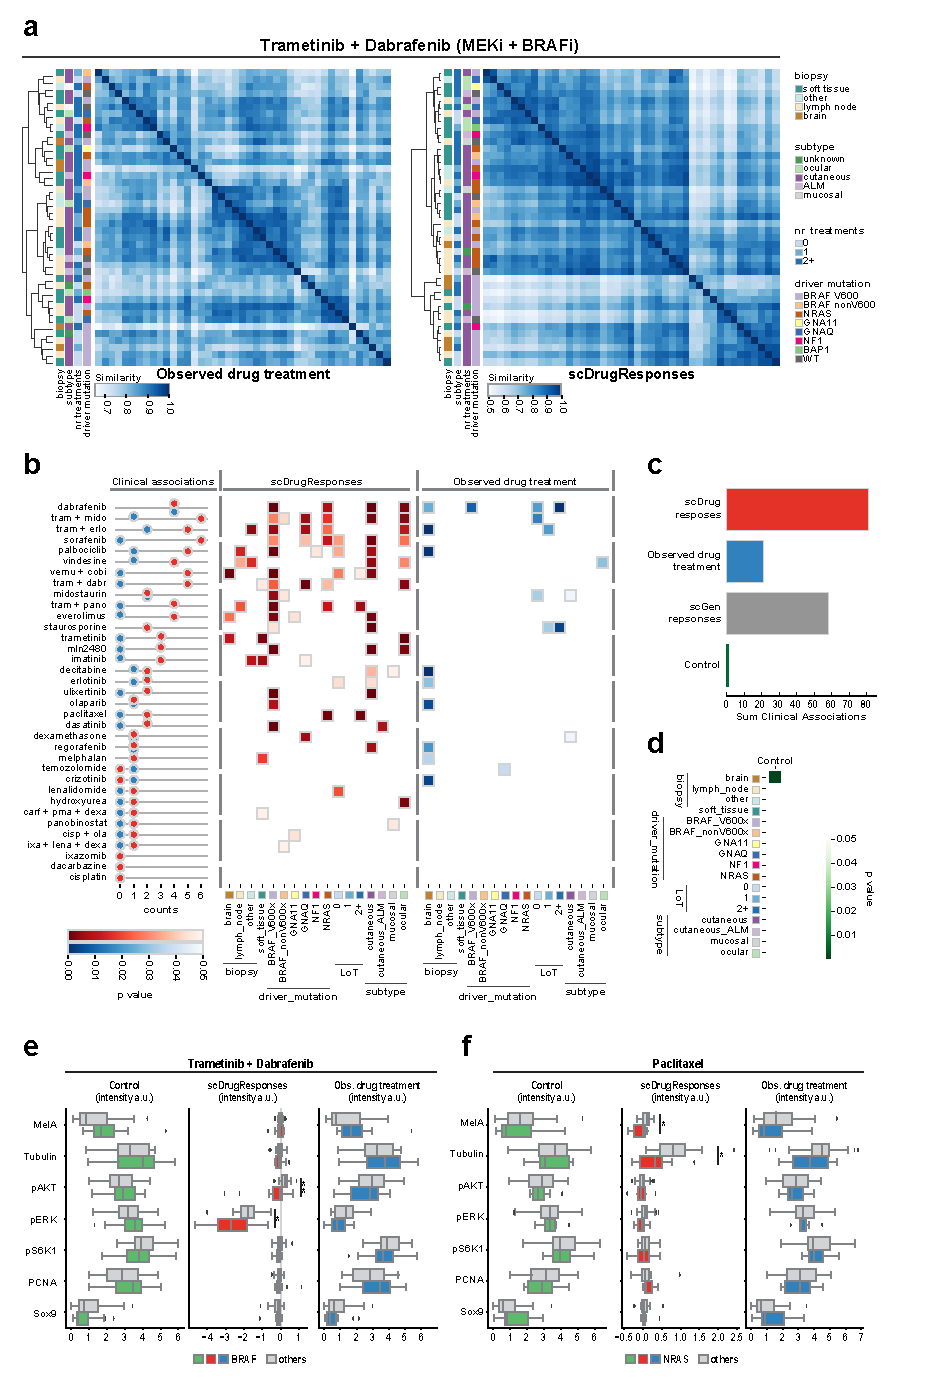
\includegraphics[width=0.65\textwidth]{figures/cellot-cohort/iid-associations.pdf}
  \end{center}
  \caption{
  Single-cell Drug Responses reveal unknown clinical associations and postulated resistance mechanisms.
a) Hierarchical clustering of patient profiles derived from Trametinib + Dabrafenib observed cells (left) and scDR predicted cells (right).
b) Associations of drug responses to clinical features. Total significant associations (left panel, p < 0.05) of scDRs (red) and observed cells (blue). Significant associations based on scDRs (middle panel) and observed cells (right panel). Darker hues indicate more significant associations.
c) Sum of identified clinical associations across all drug treatments for other data modalities.
d) Clinical associations detected using control cell features.
e) and f) Clinical associations detected across three cellular representations and differential responses of relevant driver mutations, Tram+Dabra and BRAF (e) and Paclitaxel and NRAS (f).
}
  \label{fig:iid-associations}
\end{figure}
% TODO: text

Clearly, scDR gave us access to previously inaccessible descriptions of cellular processes in patient samples.
 Our aim was now to develop suitable patient-level descriptors based on scDRs to discover differential drug responses associated with clinical characteristics of patients.
 For our benchmarking effort, we introduced MMD as a similarity measurement between two sets of multi-dimensional distributions.
 We extended the concept to perform pairwise patient comparisons of scDR and treated-predicted profiles.
 As a proof-of-concept, we decided to use our approach to compare the drug responses of our patients to Trametinib + Dabrafenib, a well know targeted therapy for patients with a BRAF alteration as their driver mutation.
 
We performed hierarchical clustering on the patient similarity matrix generated using either observed-treated or scDR profiles and visualized the clinical data associated with each sample as row labels between the dendrogram and the similarity matrix (Figure \ref{fig:iid-associations}a, Methods).
 We found that clustering samples based on observed-treated profiles failed to reveal driver mutation-associated patient groups (Figure \ref{fig:iid-associations}a, left panel).
 The clustering of samples using scDRs on the other hand, resulted in patient groups with very distinct clinical profiles (Figure \ref{fig:iid-associations}a, right panel).
 At the very bottom of the similarity matrix, we found a group of samples primarily harboring a BRAF V600 driver mutation, validating our initial expectation of differential drug responses in BRAF and non-BRAF mutated tumors.
 Unexpectedly, scDR-based patient profiles revealed further patient groups such as one dominated by samples with NRAS mutations or a third one made up of mostly of samples of ocular subtype.
 This first comparison confirms, that scDRs contain previously inaccessible biological information that links ex-vivo drug responses to clinical patient information.
 Further, this new modality allows for the investigation of differential drug depending on clinical subcohorts. 

Intrigued by these strong associations, we extended our analysis to all drugs of our 4iDRP platform by developing an algorithm that identifies the overrepresentation of clinical features within a patient group using a hypo-geometric test.
 We found that for all but two drugs, scDRs-based profiles led to the identification of more clinical associations (Figure \ref{fig:iid-associations}b, Supplementary Figure \ref{need}), resulting in over 80 known and unknown associations detected by scDR in our dataset (Figure \ref{fig:iid-associations}c).
 Surprisingly, the unperturbed state (control) of tumor cells only revealed differences between samples derived from the brain and other biopsy sites (Figure \ref{fig:iid-associations}d), highlighting the striking differences in tumor biology between brain metastases and metastases of other locations \cite{31} as well as reaffirming the need to compensate for underlying heterogeneity in order to accurately measure drug responses.  

In line with our qualitative findings for Tram+Dabra, our quantitative approach found associations related to driver mutations and subtypes in scDR profiles but failed to find any significant associations in the observed-treated setting (Figure \ref{fig:iid-associations}b).
 Importantly, patient profiles generated by another state-of-the-art single-cell prediction algorithm failed to identify the said associations too (Supplementary Figure \ref{need}).
 We decided to investigate the differential response of BRAF-mutated patients further by comparing their 4iDRP readouts to the rest of the cohort (Figure \ref{fig:iid-associations}e).
 We found 2 4i measurements, pERK and pAKT, to significantly differ between the groups when using scDRs and no significant differences between the two subcohorts in the other two modalities (Control and ODT).
 pERK was reduced in both groups, but showed a stronger reduction in the BRAF-mutated samples, in line with the intended use for patients with a BRAF mutation.
 Intriguingly, the treatment led to a reduction of AKT phosphorylation in the BRAF-mutated samples, whilst it increase levels of pAKT in the other samples.
 This differential response recapitulates extensive findings about a PI3K-mediated escape mechanism in Melanoma​32,33​ and reaffirms the need of a coordinated de-activation of MAPK and MTOR pathways to achieve clinically meaningful treatment responses. 

We, also found unexpected and unreported associations such as a differential treatment response of NRAS-mutated samples to Paclitaxel (Figure \ref{fig:iid-associations}b).
 Paclitaxel is a chemotherapy approved in the early nineteen-nineties which induces cell cycle arrest and apoptosis in proliferating cells by preventing depolymerisation of microtubules \cite{34}.
 Fittingly to its MoA, we found upon further investigating of the drug response that NRAS-mutated samples had a reduced Tubulin accumulation compared to the rest of the cohort which was independent of the respective control states and statistically undetectable in the observed-treated measurements (Figure \ref{fig:iid-associations}f).
 This finding points towards attenuated efficiency of Paclitaxel in NRAS-mutated patients, which may serve as the foundation for further experimental and clinical evidence gathering.
 Identifying treatment options which are of particular benefit to patients with NRAS-mutated tumors would be of particular value since NRAS is the second most prevalent genetic alteration in Melanoma (16.4\%), currently lacks targeted therapies and is associated with overall poorer health outcomes \cite{35}. 

Taken together our results show that scDR is a novel modality more apt at identifying previously known as well as unknown differential drug responses compared a traditional approach using measured treatment effects.
 We further show that the detected differences are often linked to the postulated MoA of the studied drugs, and thus could serve as a hypothesis generator to further refine the use of targeted and chemotherapies to subcohorts of progressed melanoma patients.  

\begin{figure}[h]
  \begin{center}
    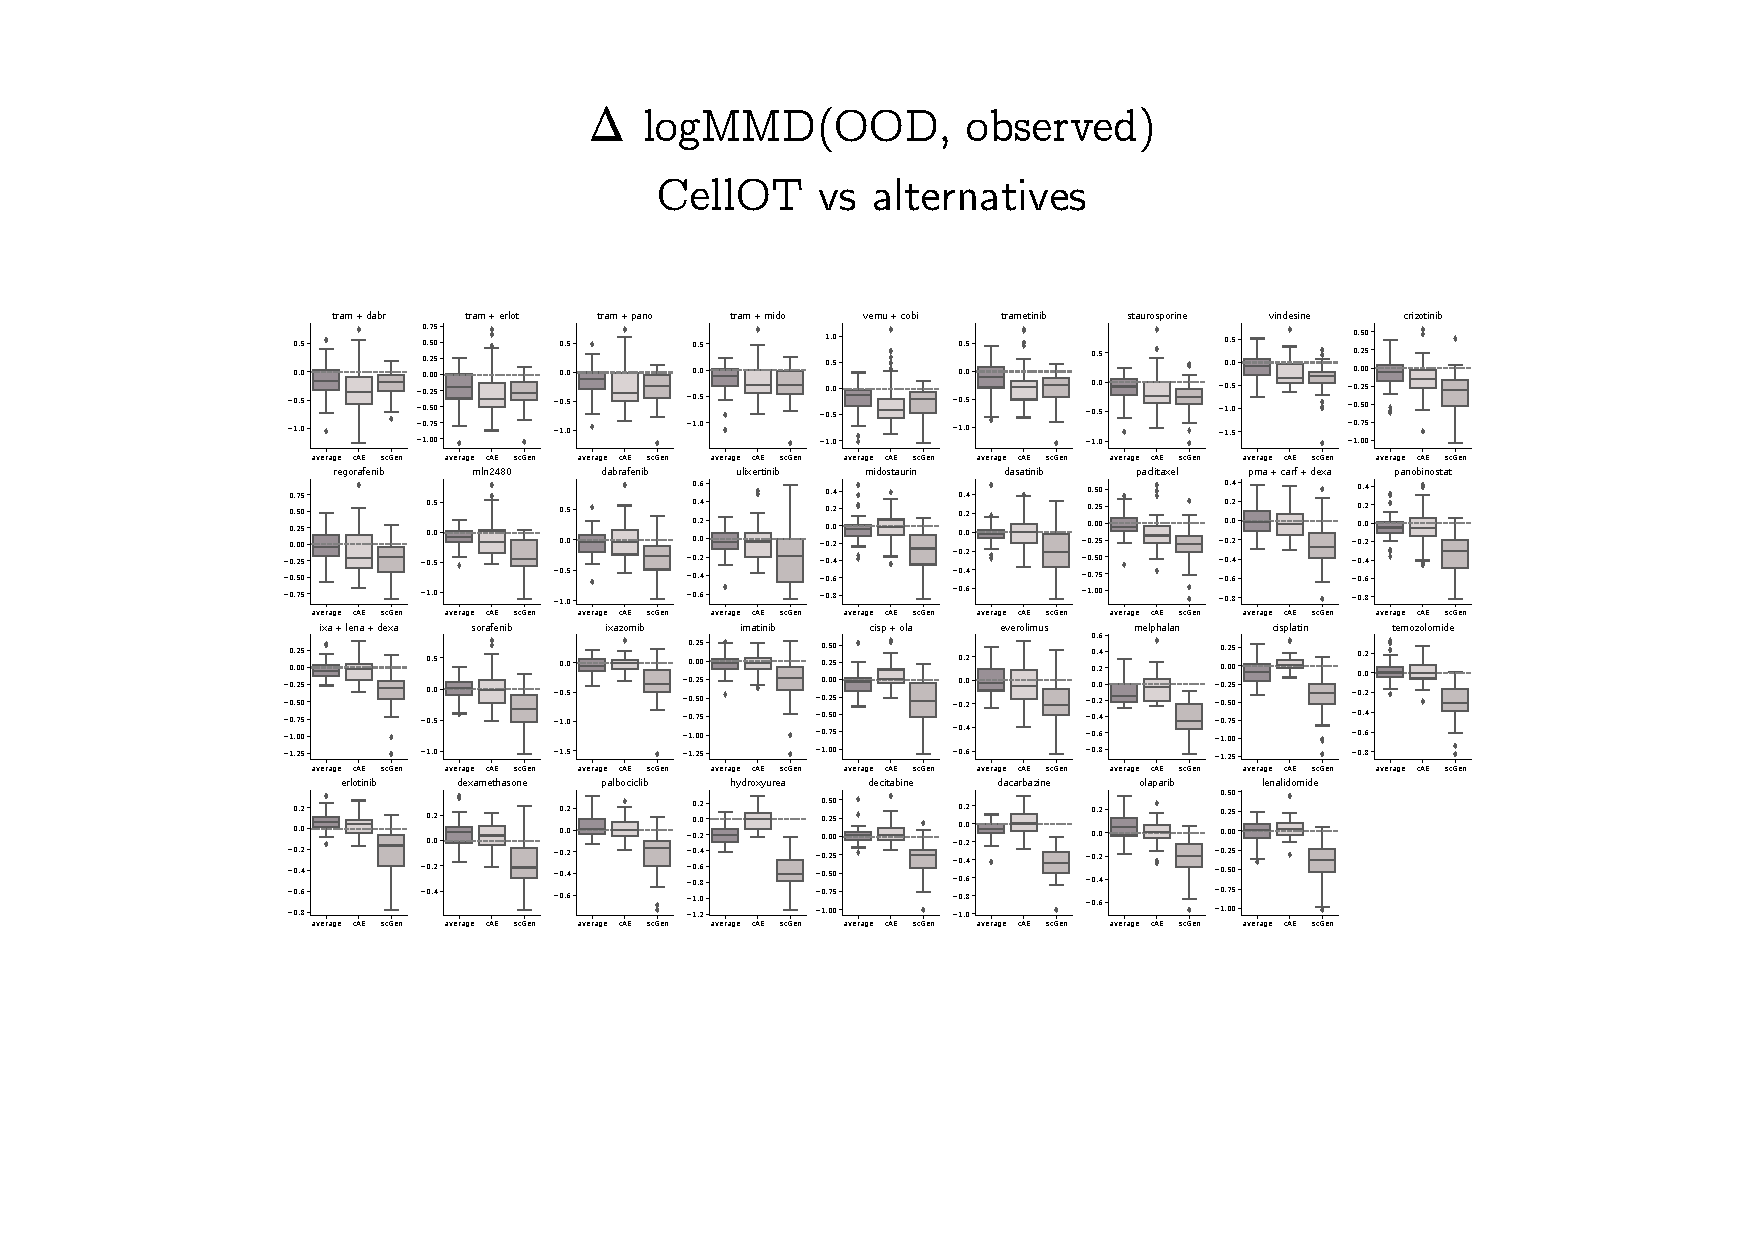
\includegraphics[width=0.95\textwidth]{figures/cellot-cohort/ood-eval-logmmd.pdf}
  \end{center}
  \caption{
    Pairwise logMMD differences comparing $\textsc{CellOT}$ and baseline approaches.
    For each (drug, patient) pair, models are trained on the entire cohort with that patient held out.
    Each model predicts the drug response of the heldout patient
    and logMMD values are computed between the distribution of predicted treated states and the true treated states.
    Negative values correspond to settings where $\textsc{CellOT}$ improves over the corresponding baseline.
  }
\label{fig:ood-eval-logmmd}
\end{figure}

\begin{figure}[h]
  \begin{center}
    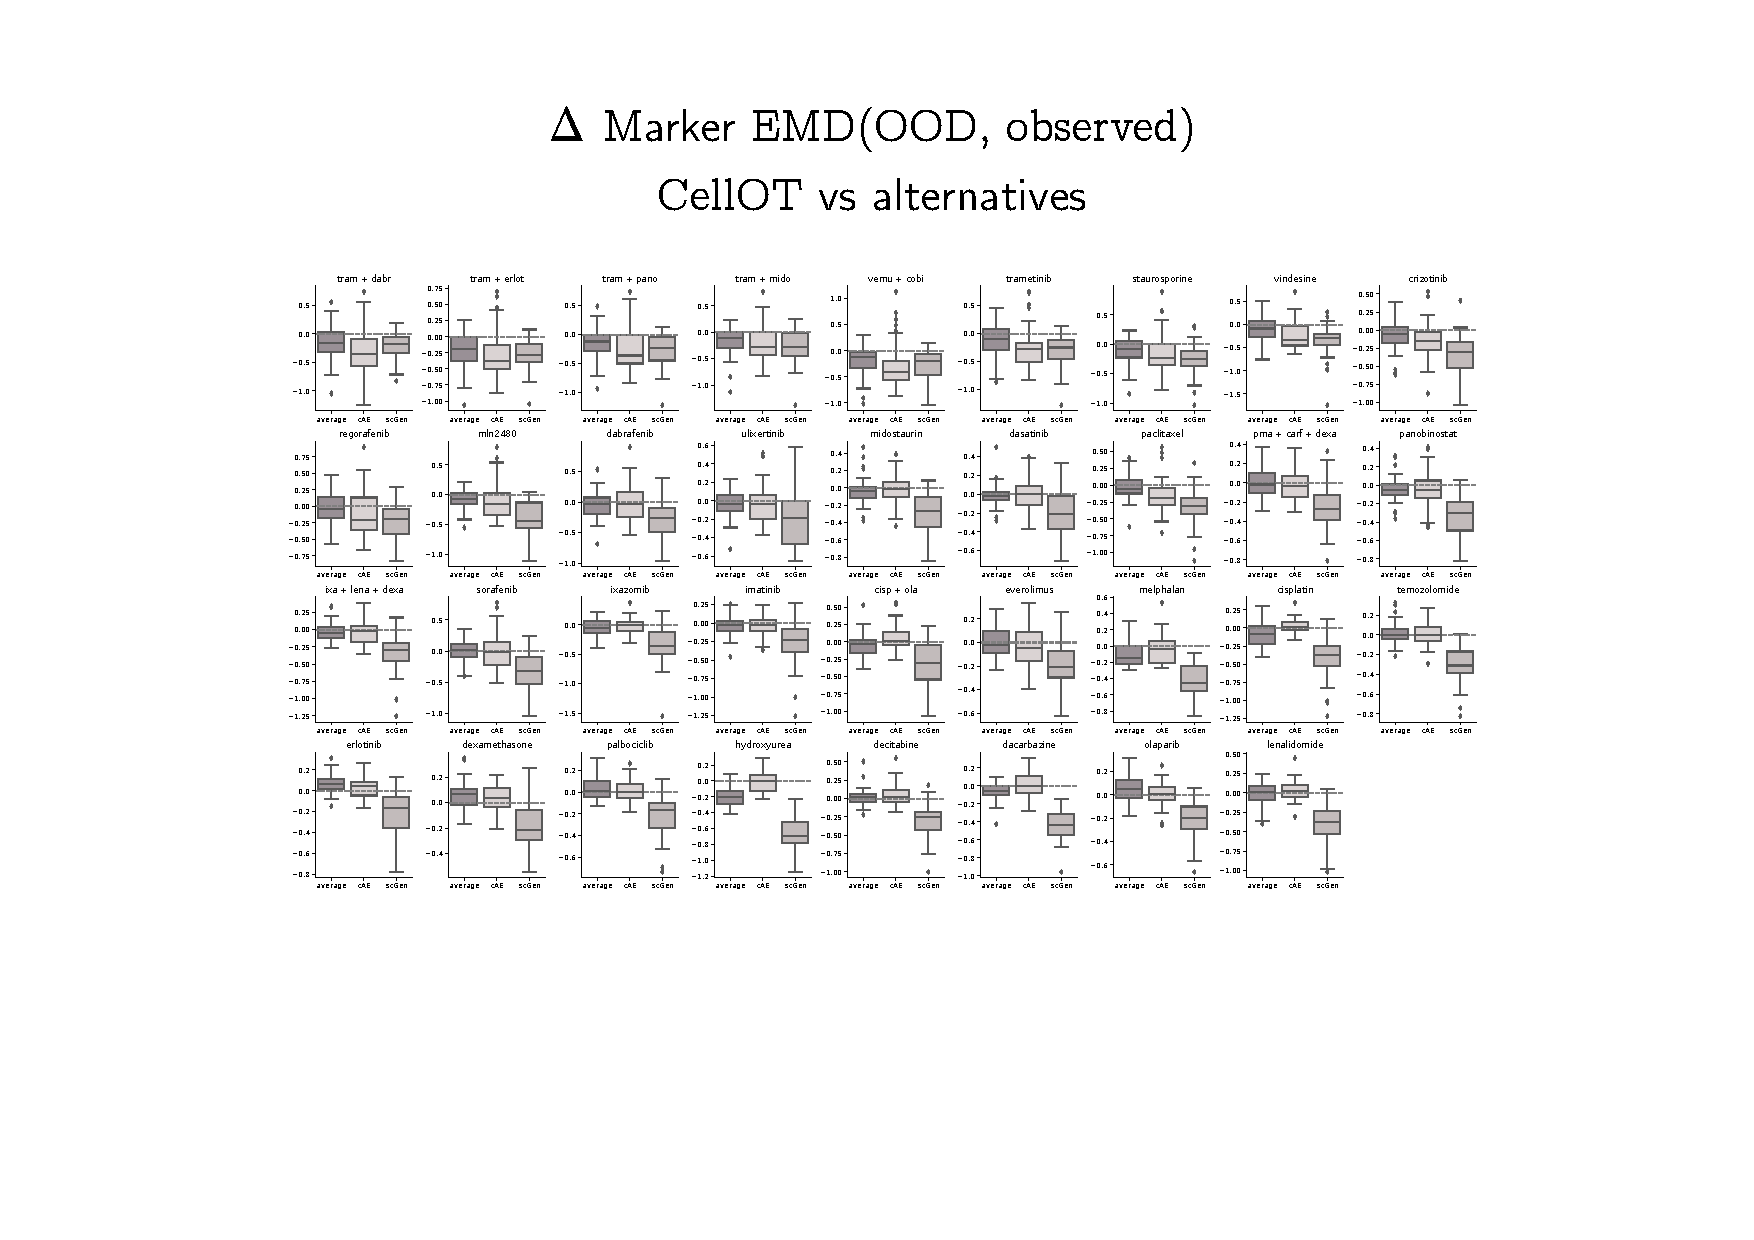
\includegraphics[width=0.95\textwidth]{figures/cellot-cohort/ood-eval-marker.pdf}
  \end{center}
  \caption{
    Pairwise marker EMD differences comparing $\textsc{CellOT}$ and baseline approaches.
    For each (drug, patient) pair, models are trained on the entire cohort with that patient held out.
    Each model predicts the drug response of the heldout patient
    and marker EMD values are computed between the distribution of predicted treated states and the true treated states.
    Negative values correspond to settings where $\textsc{CellOT}$ improves over the corresponding baseline.
  }
  \label{fig:ood-eval-marker}
\end{figure}

\begin{figure}
  \begin{center}
    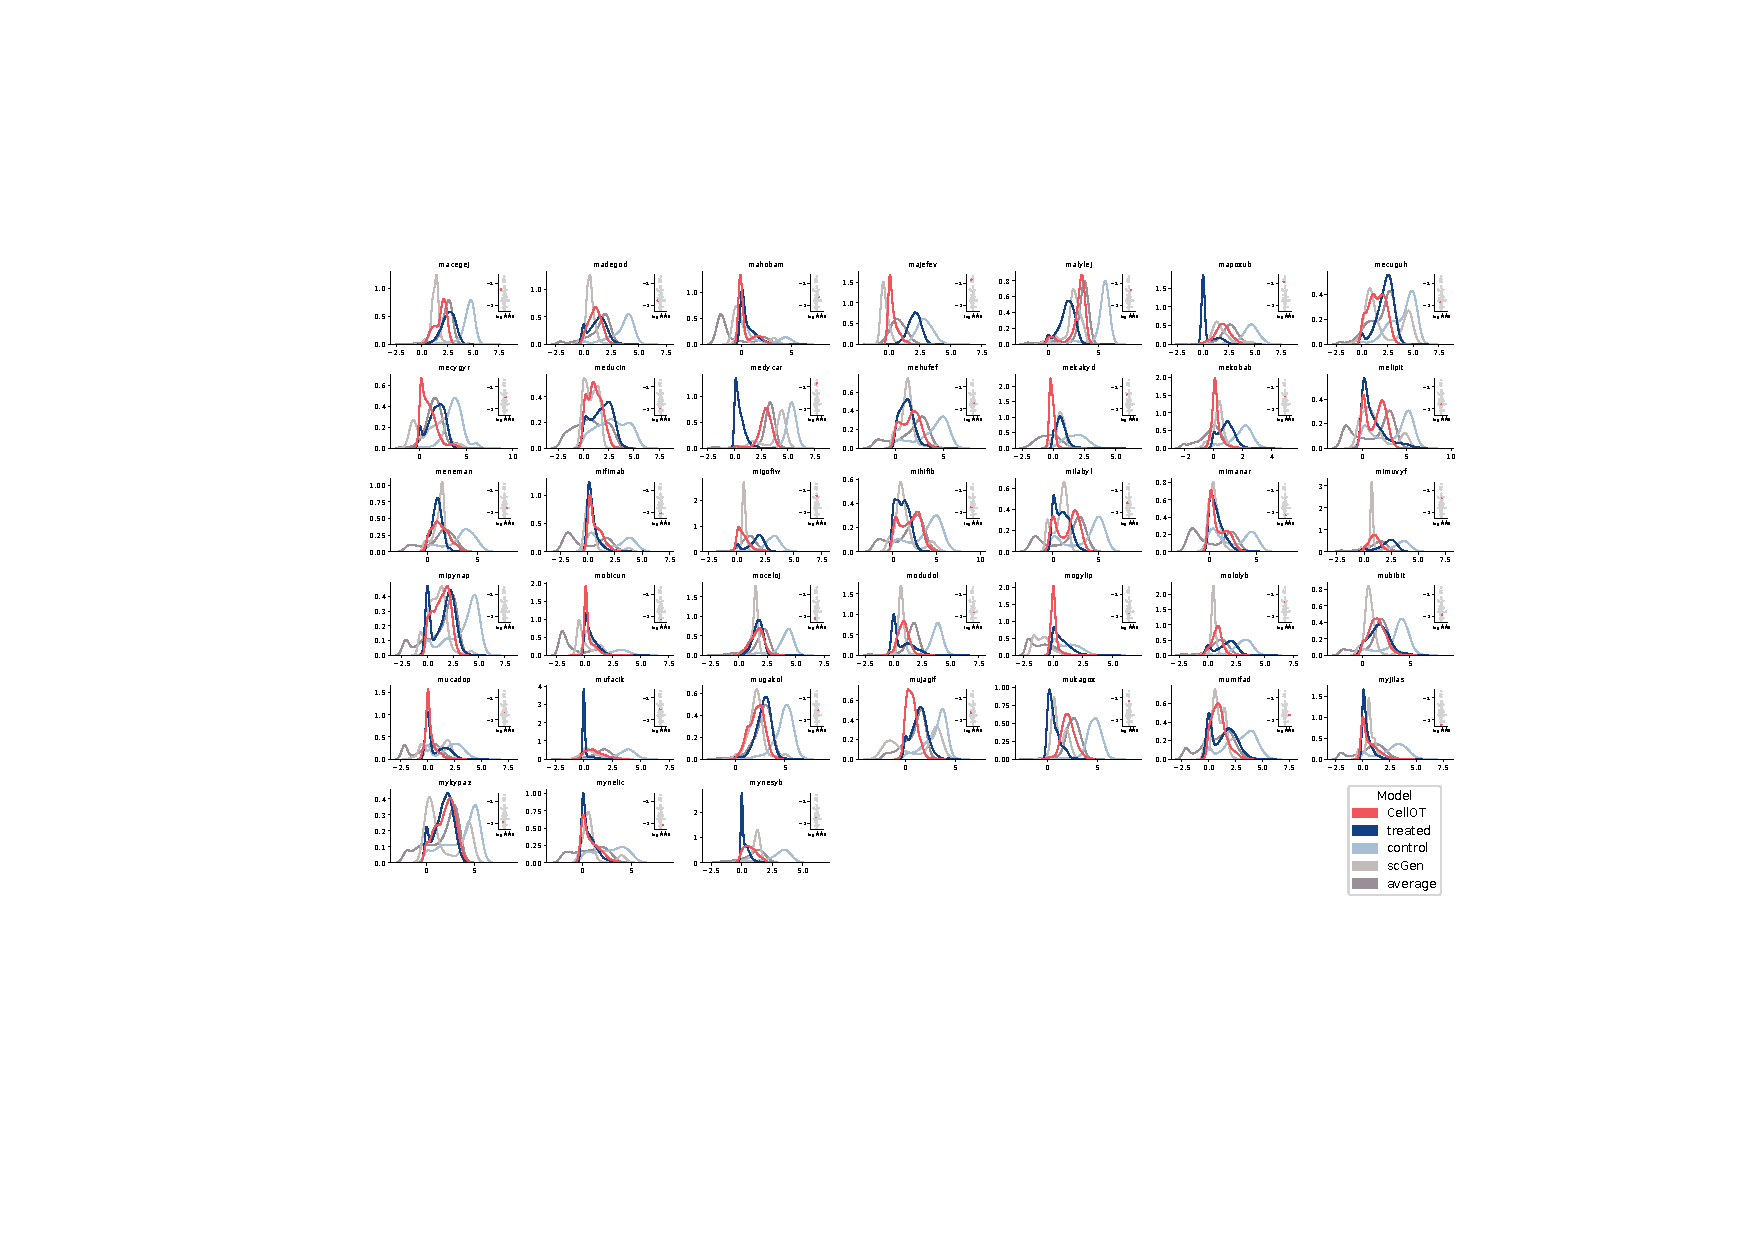
\includegraphics[width=0.95\textwidth]{figures/cellot-cohort/ood-predict-marginals.pdf}
  \end{center}
  \caption{
    Predicted response to trametinib dabrafenib combination treatment of each heldout samples.
    Marginals are shown for the treatment's marker feature, pERK.
    The inlay shows the selected heldout sample's logMMD score against the rest of the cohort.
  }\label{fig:ood-predict-marginals}
\end{figure}

\begin{figure}
  \begin{center}
    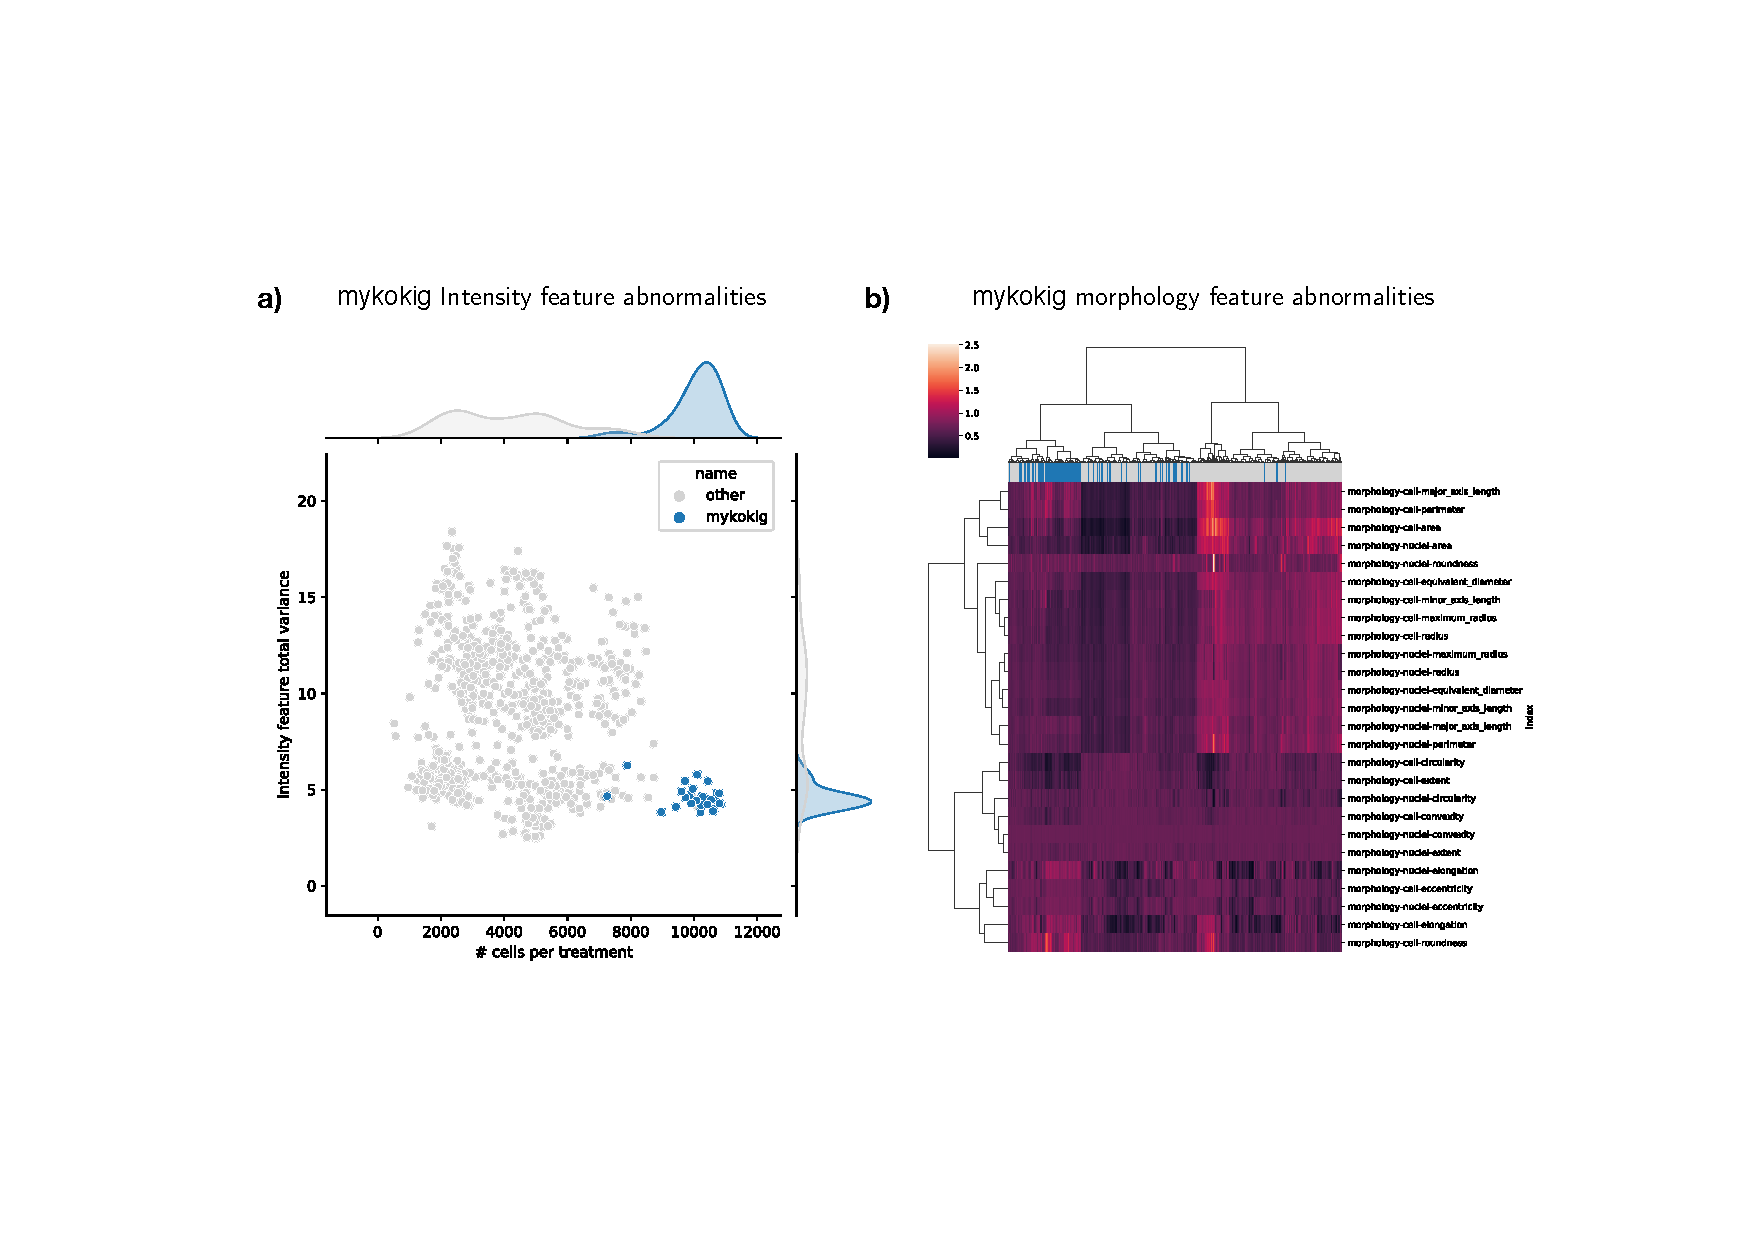
\includegraphics[width=0.95\textwidth]{figures/cellot-cohort/progression-exclude-mykokig.pdf}
  \end{center}
  \caption{
    Sample mykokig exhibits evidence for low quality cell segmentation and is removed from the progression prediction task.
  a) Scatter plot of number of treated cells by the variance of intensity features.  Each dot corresponds to a (treatment, sample) pair and treatments of mykokig are shown in blue. Mykokig behaves as an outlier as it has much more cells per treatment than other samples and these cells have low variance in their intensity features.
  b) Morphology features of mykokig cells indicate the presence of artifacts. The cluster map shows the distribution of each extracted morphology feature (rows) for cells sampled from mykokig and a subset of 5 samples from the full cohort. A large fraction of mykokig cells exhibit a strange unique morphology pattern of small round cells.
  }\label{fig:progression-exclude-mykokig}
\end{figure}

\begin{figure}
  \begin{center}
    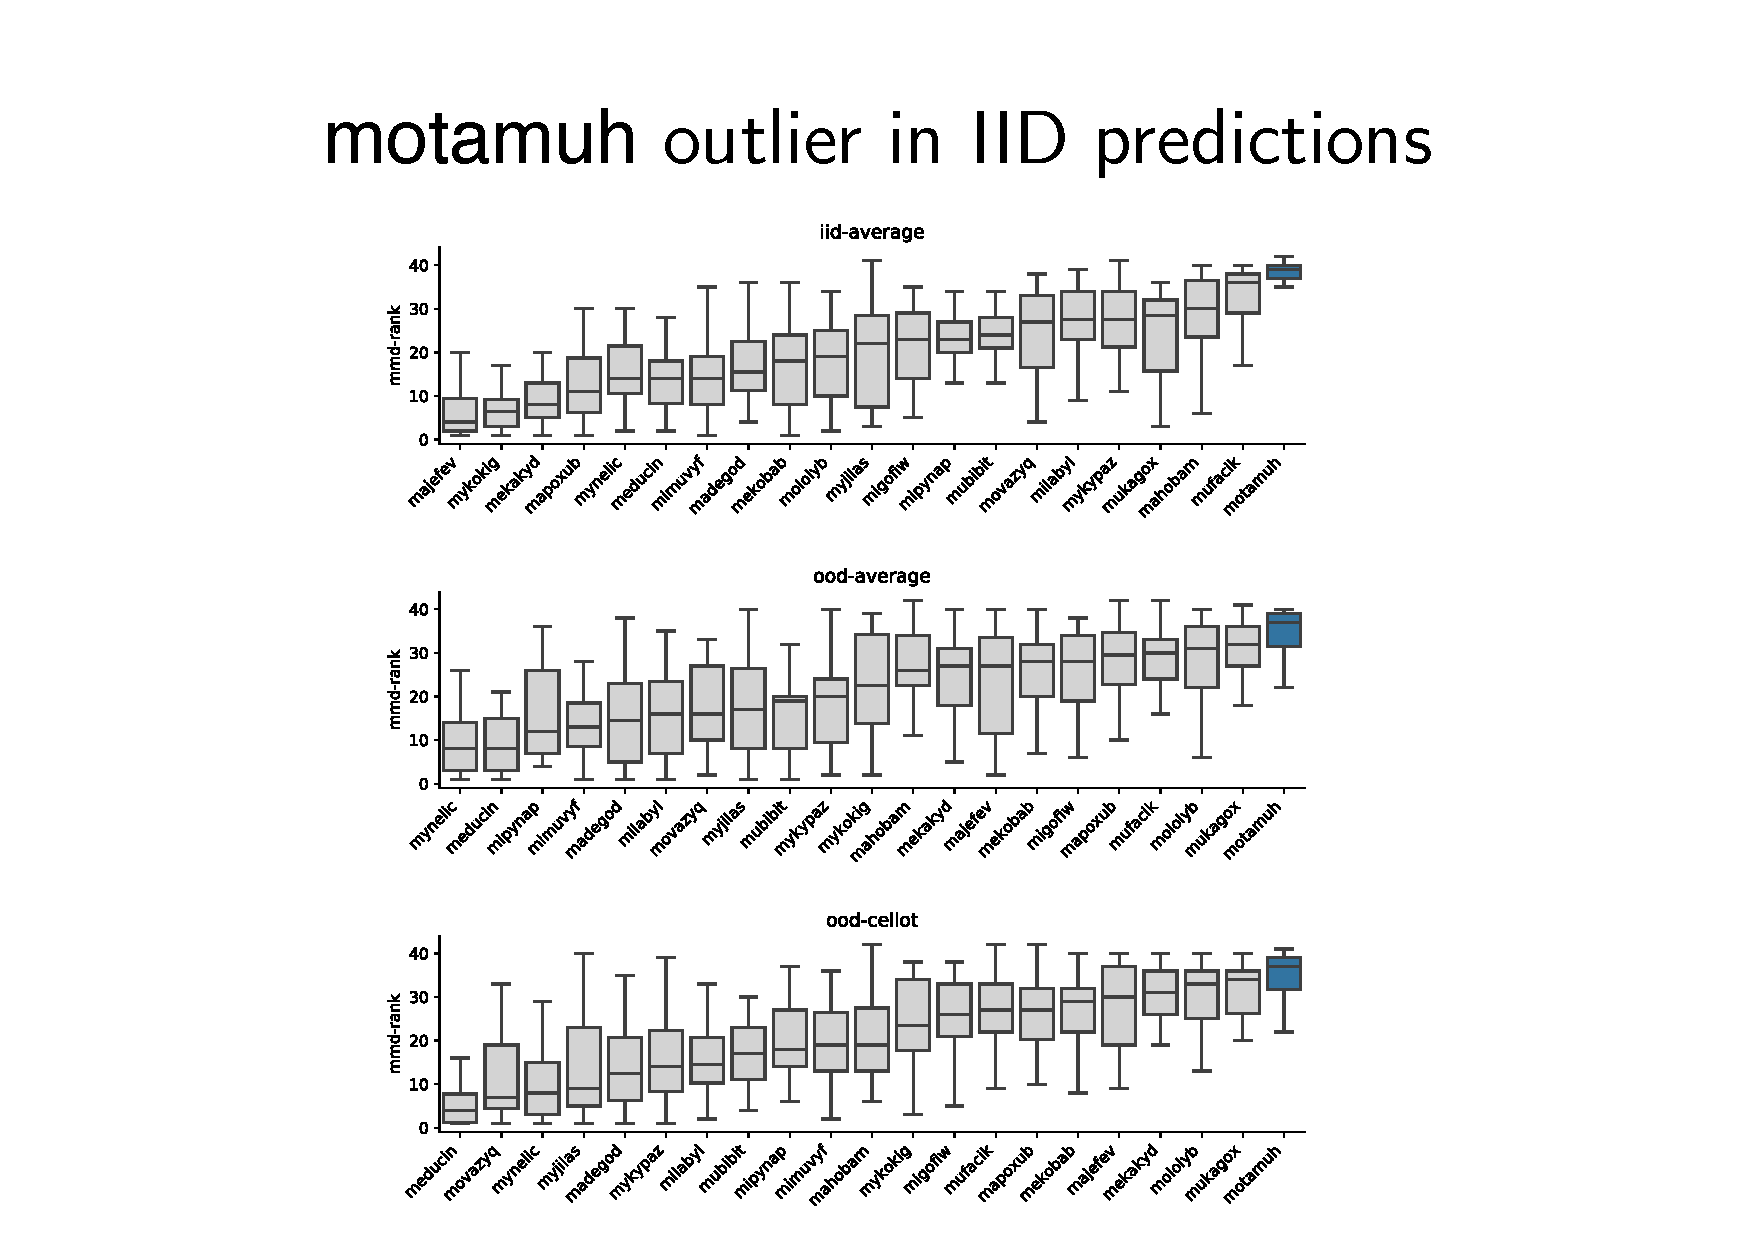
\includegraphics[width=0.95\textwidth]{figures/cellot-cohort/progression-exclude-motamuh.pdf}
  \end{center}
  \caption{
    The predicted responses for sample motamuh are consistently poor and the sample is therefore removed from the progression prediction task.
    Boxplots show the ranked MMD metric computed between each model's prediction and observed treated states for drugs considered in the progression prediction task.
    Results for the average model are shown in the IID and OOD setting as well as CellOT predictions in the OOD setting.
    Sample motamuh consistently ranks worst across all samples in the cohort for these prediction tasks.
  }\label{fig:progression-exclude-motamuh}
\end{figure}

\subsection{OOD performance}
\begin{figure}[ht!]
  \label{fig:ood-main}
  \begin{center}
    \includegraphics[width=0.95\textwidth]{figures/cellot-cohort/ood.pdf}
  \end{center}
  \caption{
    a) Generalization to heldout samples. For each patient, for each drug, we hold that patient out and train a model on the combined set of observed control and treated cells of the rest of the cohort.
    b) Predictions are made on the held out patient for each (patient, drug, model) triplet and metrics are computed between the responses and predictions of the unseen held out patient.
    We report significant differences (t-test, $p < 0.01$) to each baseline model as colored boxes. Blue hues indicate significant improvements.
    The relative treatment strengths, computed as the metric between the observed control and treated cells, are reported as purple column colors.
    c) Selected predicted marginals of marker features.
    The distribution of CellOT-predicted MMD scores is shown in the inlay, highlighting the selected sample.
    d) Predicting the progression status of incoming samples at 90 days using predicted cellular responses.
    Given access to a training subset of the cohort, IID-predicted cellular responses are clustered and a binary SVM is trained to classify progression status within 90 days using sample level cluster frequencies.
    Incoming samples are predicted using the \emph{OOD}-predicted cellular responses, i.e. without observations of treated states.
    e) kMeans cluster (k=10) centers of marker intensities cellular responses (left) and the cluster frequencies of each sample (right).
    Column colors correspond to the progression label, misclassification rate, and the known days to progression. Samples close to the cutoff are misclassified.
    f) Accuracy to predict progression status within 90 days of incoming samples.
    We compare against similar approaches which represent cells as their predicted treated state, the observed control state, and a random forest on relevant sample metadata.
  }
\end{figure}

In order to simulate the clinic environment, we construct, for each patient, a training set composed of all other patients in the cohort (Fig \ref{fig:ood-main}a).
Then, for each perturbation available,
we train a model on the control and treated cells across the whole observed cohort
and apply this model to predict the responses of the unseen patient.
We then evaluate the set of predicted cellular states against the unseen treated cells of the held out patient, as we had done in the iid case.
In addition to the MMD metric, which considers the state of a multi-dimensional cellular feature set,
we also report the Earth Mover’s Distance (EMD) of the marker feature of each perturbation.
The marker feature is selected by computing the EMD of the observed control and treated states and selecting the feature with the highest average distance,
i.e. the feature that was most affected by the perturbation.
For instance, for Trametinib, this feature is pERK.
The marker feature is of particular interest to the clinician as this typically corresponds to the cellular pathways the treatment is designed to control.

Within each treatment, we compare the ability of CellOT to consistently improve predictions of heldout samples across the whole cohort against baseline approaches.
Fig \ref{fig:ood-main}b shows for which treatments there are significant differences across the whole cohort between
the metric reported by CellOT and the baseline approach, as measured by a relative t-test (p-value < 0.01).
The full distributions for the differences of these metrics can be found in Figures \ref{fig:ood-eval-logmmd} and \ref{fig:ood-eval-marker}.
We demonstrate that we are able to make strong gains in many perturbation settings, including most of the targeted therapies.
These therapies are of particular interest as they are among some of the most commonly administered treatments \cite{need} and, in addition, tend to have the strongest effects.
Many other treatments tend to have more subtle effects, wherein individual effects can dominate the response and thus generalization is difficult to attain.
However, CellOT rarely underperforms against the baselines, and in the few cases when it does, it does so with small effect sizes.
Note that while \textsc{scGen} tends to capture the response of a particular marker feature (EMD metric), it struggles to capture realistic cellular states (MMD metric), while the other baseline methods have the inverse behavior.
CellOT is able to offer the best of both, highlighting its robustness and stability.
We furthermore provide some example marginals (Fig \ref{fig:ood-main}c, full set in Fig \ref{fig:ood-predict-marginals}), showcasing how CellOT is able to learn biologically relevant states.
We include the MMD metric corresponding to the selected CellOT predictions, to give a general indication of how well the model is performing.

\subsection{Learning differential responses with conditional parameters}

\begin{figure}[h]
  \begin{center}
    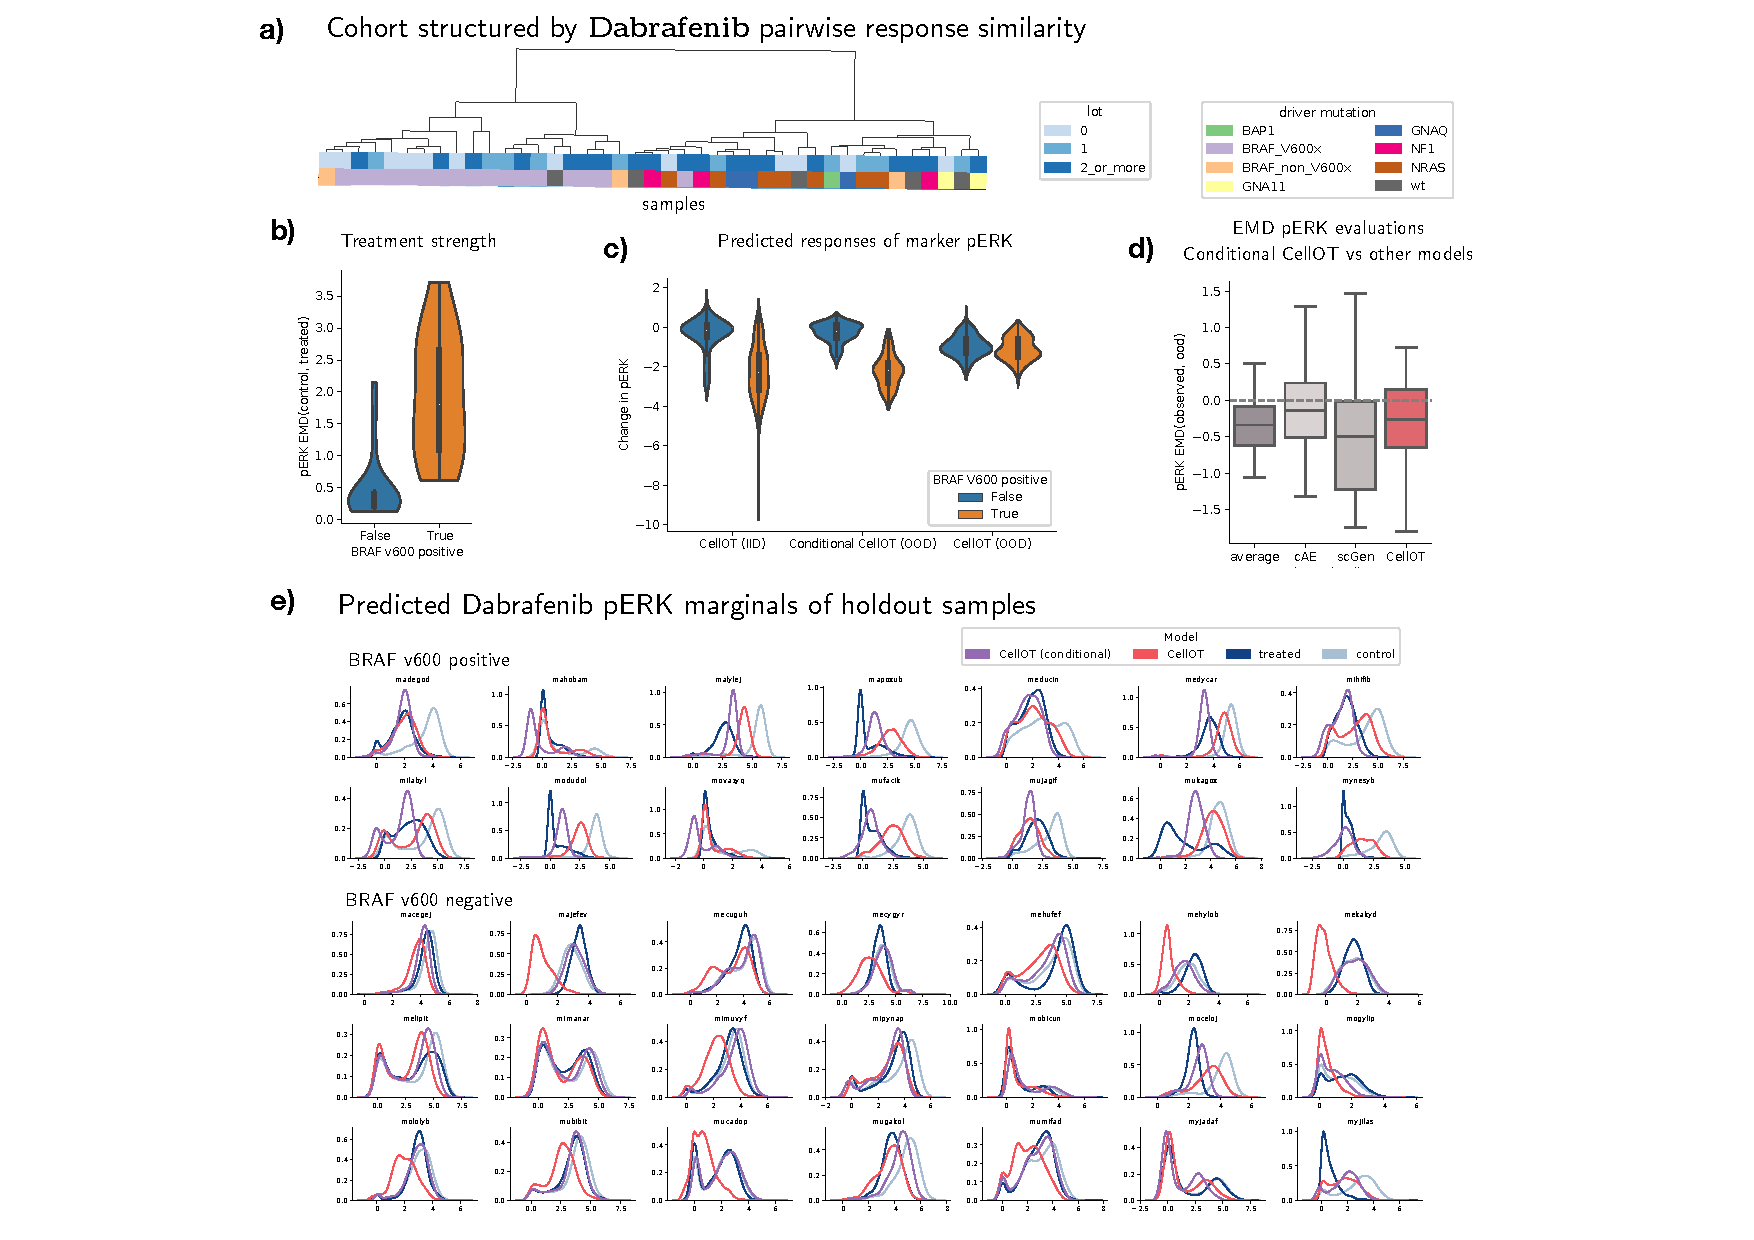
\includegraphics[width=\textwidth]{figures/cellot-cohort/condot.pdf}
  \end{center}
  \caption{
    Predicting strongly differential responses to Dabrafenib of holdout samples using Conditional CellOT.
    a) Dendrogram of sample-level pairwise similarities of Dabrafenib responses, computed using the MMD distances between each sample's distribution of IID-predicted responses reveal similarly responding clusters of non-BRAF samples, BRAF samples with no lines of treatment, and BRAF samples with at least one line of treatment.
    Samples (columns) are colored based on the number of lines of treatment and driver mutation status.
    b) Differential effect strength of Dabrafenib, measured using the EMD of its marker, pERK, between control and treated cells of samples with and without the BRAF driver mutation that the treatment targets.
    c) Predicted responses of pERK for samples with and without the BRAF driver mutation, in both IID and OOD settings.
    OOD $\textsc{CellOT}$ is not able to generalize the differential responses out-of-distribution, while the conditional model has improved performance when compared to the IID model.
    d) Improvements of the pERK marker EMD for predictions made by the conditional CellOT vs other approaches. The metric is computed on the predictions of each approach on cells from holdout samples and the pairwise differences to conditional CellOT are shown. Negative values correspond to improvements Conditional CellOT makes. 
    e) pERK marker marginals for CellOT and conditional CellOT models for BRAF positive (top) and negative (bottom) samples.
  }\label{fig:conditional-ot}
\end{figure}

A common strategy in the design of cancer therapies is to tailor the treatment to interact with some specific mechanism that fails across a number of different cancers.
These \emph{targetted} therapies would, for instance, be designed to treat patients with some driver mutation, such as the infamous BRAF driver mutation \cite{need}.
In such cases, the cellular profile might not capture information crucial to determining the nature of the response, e.g. the presense of the BRAF mutation,
and therefore $\textsc{CellOT}$ performance, as we have described thus far, may struggle.
Here we apply the framework described by \cite{need} to include sample metadata, in the form of \emph{conditional} parameters, in order to help the transport function learn such differential responses.

Here, we focus on the dabrafenib treatment, a targetted therapy to treat BRAF-positive patients.
We observe a strongly differential structure in the responses across the cohort.
Sample similarities are determined by computing the MMD between the learned (IID) single-cell responses of each pair of samples.
Fig \ref{fig:conditional-ot}a) shows a dendrogram computed over the set of these pairwise similarities where were we find three main clusters: non-BRAF samples, BRAF positive samples with no previous lines of treatment, and BRAF positive samples with at least one line of treatment.
While the differential response across BRAF status can be easily explained by the targetted nature of the treatment, the differential resposne to number of treatment lines might be due to a particularly advanced or difficult cancer that necessitates several rounds of treatment.
Fig \ref{fig:conditional-ot}b shows the differential response of pERK, the marker feature for dabrafenib, across BRAF mutation status, by computing the EMD of pERK between the control and observed dabrafenib responses.
Here we observe that dabrafenib induces a strong pERK response in patients with the BRAF mutation, but a weak response in those without,
an observation is in agreement with the intended design and use of the drug.

In order to learn the strongly differential response of dabrafenib,
we train a version of CellOT whose inputs inputs are \emph{conditioned} \cite{condot} with the status of the sample's driver mutation and lines of treatment. 
These conditional parameters are able to inform and influence its learned responses with clinical metadata
This is acheived by concatenating a one-hot encoding of each metadata to the cellular features.
Note that while the potentials trained by $\textsc{CellOT}$ must be convex in their inputs,
they do not need to be convex in these conditional inputs \cite{icnn}.

By comparing the conditional $\textsc{CellOT}$ predictions to vanilla $\textsc{CellOT}$ trained in the IID and OOD settings, we observe that the conditional version is able to better capture the differential pERK responses.
In Fig \ref{fig:conditional-ot}c) we see that the IID $\textsc{CellOT}$, which is able to learn patient-specific responses, indicates that BRAF samples respond to dabrafenib by decreasing pERK levels, while non-BRAF samples have a negligible response.
OOD $\textsc{CellOT}$, on the other hand, predicts all samples, regardless of their BRAF status, to respond to dabrafenib with a slight decrease of pERK levels, and report little to no difference across BRAF status.
The conditional $\textsc{CellOT}$, however, is able to correctly predict a differential response across BRAF status.
This is futher quantified in Fig \ref{fig:conditional-ot}d), where we see consistent improvement in OOD pERK prediction when using conditional $\textsc{CellOT}$ over vanilla $\textsc{CellOT}$ and other baseline models.
Finally, marginals highlighting the learned differential responses are shown in Fig \ref{fig:conditional-ot}e,
where it can been seen that conditional $\textsc{CellOT}$ indeed learns the pERK response of BRAF positive samples (top) and non-response of negative (bottom).

\subsection{Identifying at-risk patients from predicted cellular responses}
The ability to understand whether or not a tumor will progress quickly is of clinical importance as it is an indicator of the severity of the cancer.
In this experiment we demonstrate the clinical utility of predicted single-cell perturbation responses of incoming patients by classifying the progression status of this sample 90 days after treatment.
Here, we simulate the clinic enviornment, and assume that we have access to the control and perturbed states from a (training) cohort.
Given an incoming sample, we observe only their untreated cells, \emph{predict} their cellular responses using the OOD $\textsc{CellOT}$ maps described above, and finally identify the progression status from a model trained on the observed responses of the cohort.

\paragraph{Subcohort selection}
To ensure that we select treatments that are relevant to the situation of individual patients, we limit ourselves to the treatments that had been prescribed to samples by the medical board associated with the Tumor Profiler project.
From the total cohort, 22 samples had been prescribed a studied small molecule treatment.
Of these 22, we removed three samples due to quality control: \textsc{mykokig}, had evidence of unfiltered artifacts in its observed treated cells \ref{fig:progression-exclude-mykokig}, \textsc{motamuh}, as it represents an extreme outlier in IID and OOD response prediction tasks \ref{fig:progression-exclude-motamuh} , and \textsc{mecygyr}, as it had showed evidence of immediate progression at the start of the study ( $<$ 5 days), leaving a subcohort of 19 samples.
Of these 19, 9 progress within 90 days and 10 do not, which yields a balanced binary prediction task.
We simulate the clinic environment by splitting the patients into a train (75\%) and test (25\%) set, (i.e. within each split, 4 of the 19 samples are heldout), where we have access to the control and treated cells of all patients in the training set, and can only access the control cells of patients in the testset.

\paragraph{Prediction model}
Our prediction model, summarized in Fig \ref{fig:ood-main}d, works as follows: first, single-cell responses are clustered and patients are represented as frequencies over these clusters, and then an SVM classification model is trained to predict the binary progression status using the patient representations.
To construct the patient representations of the training set, a KMeans clustering is computed using the single-cell treatment responses from all patients in the training set, as predicted using the IID CellOT models \ref{}.
We perform a soft assignment of each cell to the k cluster centers, via a softmax transformation over the negative distances to each cluster center, to smooth cluster assignments and help include a notion of cluster similarities, Fig \ref{fig:ood-main}e left.
After this step, each cell is now represented as a probability over the set of cluster centers, Fig \ref{fig:ood-main}e right.
A patient-level representation is constructed by averaging the cluster assignments over all cells from each patient.
At test time, the OOD-predicted cell responses are used instead of the IID, as we are unable to access their treated cell states.
The predicted responses are mapped to the cluster centers, the sample frequencies are computed and the held out sample is classified with the SVM.
Note that the visualizations in Fig \ref{fig:ood-main}e are constructed on IID responses of all samples in the subcohort.
Within each split, these structures are re-computed on the training set only.

\paragraph{Evaluation}
Since this is a balanced classification task, we report accuracy as our metric and consider 50\% a trivial lower bound.
For each model setting we perform 100 75\%-25\% train-test splits, i.e. in each split, 4 of the 19 samples are heldout.
We include a model that predicts the progression stats at 90 days with meta information at the sample level, specifically a random forest over the subtype, lines of treatment, and known driver mutation, represented as the concatenation over one-hot encodings of each category.
We furthermore compare our approach to a similar approach that uses predicted treated states, control cells, and single-cell responses predicted by the baselines \ref{}.

The prediction accuracy of holdout samples over 100 train-test splits are shown in Fig \ref{fig:ood-main}f, where we compare using single-cell responses to using control and (predicted) treated states.
In addition, we include a random forest model trained on relevant metadata information, the sample’s subtype, known driver mutation and lines of treatment.
% TODO: fill with actual numbers
The random forest trained on sample metadata and SVM classification using control states only struggle to peform, yielding accuracies of XXX +/- XX.
The SVM classification using treated states fares slightly better, reporting accuracies of XXX +/- XX.
We see the most drastic improvement using \emph{response} information, which reports accuracies of XXX +/- XX.
% TODO: add fig
Comparisons to the autoencoder approaches as well as ablations over the number of clusters can be found in Fig \ref{}, where we show specifically that $\textsc{CellOT}$ responses are stable with respect to classification parameters and out perform baseline approaches.

A benefit of using a straight-forward clustering approach is the ability to interpret the behavior of the model.
We can interpret the decisions made by the model by analyzing the cluster means and patient frequencies over them shown in Fig \ref{fig:ood-main}e.
Here, progression status at 90 days and the misclassification rate of test set samples are shown as row colors.
We see that cells from cluster 5 exhibit a general non-response to the selected perturbations.
Furthermore, samples that have high representation of these responses are more likely to progress,
while samples that exhibit higher degrees of heterogeneity in response are shown to have a better progression status.


% !TeX root = ../../main.tex
\section{Discussion}
In this study, we introduced the 4iDRP platform, a next-generation ex-vivo functional platform operating seamlessly as part of the Tumor Profiler project in the clinical workflow of cancer care and explored the clinical utility of optimal transport based cellular responses powered by \textsc{CellOT}.
Unlike various other drug profiling efforts, 4iDRP focuses on acute phenotypic cellular responses to drug treatments rather than a cell viability measure after prolonged drug exposure. 
Accordingly, our multiplexed, 4i-based measurements capture cell physiology features aimed at generating information-rich sinmgle-cell profiles suited for reverse translational efforts as wells as clinical event predictions. 

Our findings underscore the critical challenge of patient-to-patient heterogeneity and intra-sample single-cell heterogeneity in generating functional omics data from solid oncology samples.
While the need to account for underlying variability in the control state has been well established \cite{icgc2020},
our work demonstrates that extending these concepts to clinically oriented efforts is both necessary and beneficial.
We do so here with the first-ever application of a neural-optimal transport on clinical samples and develop the concept of single-cell Drug Responses (scDRs), a novel functional data modality that captures the high-dimensional response of individual cells to treatments.

A major limitation of the current work stems from the size of the cohort.
Although this is one of the largest cohorts measuring patient responses to cancer treatments, \textsc{CellOT} and other methods applied here are able to scale to, and benefit from, much larger cohort sizes.
In particular, these limitations are most apparent when predicting the responses of an unseen patient from the observed responses of the rest of the cohort.
While we rarely fail to improve over other approaches, as the drug effects become weaker in this task we are unable to show strong gains over even trivial approaches.
We attribute this to the discussed cohort heterogeneity,
where, in these treatments, sample-specific effects begin to outweigh drug responses and generalization becomes not feasible.
We believe that as cohort sizes grow, more information that govern such sample-specific effects could become available and improve prediction performance.
Scaling could furthermore be improved through the automatization of the 4i protocol through a dedicated enclosed system, as well as simplifying sample access in the clinical routine.
Our results show that doing so could have immediate benefit to patients in hospitals and for reverse translational research of the biomedical community at-large.  

%scDRs afford unprecedented mechanistic insights into drug responses compared to previous, non-multiplexed data. Nonetheless, 4i remains a targeted omics approach, capable of observing only a subset of the biology in our samples. For this study we honed our 4i panel to measure pathways mostly affected by targeted therapies. As a trade-off the platforms ability to measure markers involved in responses to other treatment types might have been blunted. Alternatively, omics methods with more encompassing readouts such as single-cell RNA sequencing functional profiling could be [Mention other omics approaches to measure analytes wholistically (RNAseq), and counter with prohibitive cost and inability to directly measure pathwayacivity]. Generating scDR using 4i or otherwise we’ll remain slow and costly - compared to other simpler functional measurements - for the foreseeable future. We believe that rather than Rather than  modular machine-learning framework capable of incorporating and learning from independently generated, non-feature-overlapping datasets  
%
%Multimodal  

A promising approach to improve the predictive power of single-cell responses is to utilize information from multi-modal profiling or spatial contexts.
In the context of \textsc{CellOT}-powered predictions, we envision two potential avenues to incorporate such information.
Information available only on untreated cells can be considered as cell-level metadata and conditioned on, in a similar fashion to sample-level metadata.
Other spatial and multi-modal profiles available both before and after treatment can be incorporated by learning integrative representations \cite{lotfollahi2019, cao2022a}.
These methods aim to represent cells such that they contain information across multiple profile modalities, which can be relevant towards determining disease behavior.
Using these models, response prediction can proceed in the representation space, which can be mapped back to data space, as we have demonstrated previously \cite{bunne2023}.
Single-cell foundation models \cite{theodoris2023,cui2024,ma2024}, which utilize cutting edge architectures that have had major success in modeling the complexities of language \cite{vaswani2023, devlin2019, openai2024},
promise to improve cellular representations with nuances that these architectures would be able to capture.
With these improved and nuanced representations, the ability for response predictions to handle complex heterogeneous behavior will be essential, a characteristic at which neural-OT approaches like \textsc{CellOT} excel.


The integration of scDRs into clinical workflows represents a significant advancement in precision oncology, offering a powerful tool for both translational research and personalized cancer care.
The findings highlighted in this work demonstrate the need for continued development of sophisticated computational models and experimental approaches to harness the full potential of ex-vivo drug profiling, ultimately improving treatment outcomes for patients with advanced cancers. 

% !TeX root = ../main.tex

\chapter{Concluding Remarks}
%\begin{enumerate}
%  \item developed methods to align single cell populations
%  \item enhance the potential of profiling technologies
%  \item destructive/consuming nature of technologies
%  \item address limitation of single state observations
%  \item recover multiple observations through the alignment of datasets
%  \item both multi-modal integration and perturbation resposnes
%  \item applied these methods to several real world settings
%  \item including the clinic where we demonstrated the potential to improve care
%\end{enumerate}

In this thesis, we developed and applied methods that align single-cell populations to enhance the potential of single-cell profiling technologies.
While single-cell profiling technologies have revolutionized the way we are able to study cellular biology, providing observations of individual cells,
they are limited in the sense that they typically require the profiled cells to be consumed or otherwise destroyed.
Many fundamental problems in biology wish to be addressed by observing the same cell across multiple contexts, such as different modalities or points in time.
%We have come to understand cellular states as composed of many different levels, e.g. genetic state, transcriptomic state, proteomic state, etc,
%and these technologies are only able to measure cells typically within the context of one of these modalities.
%Furthermore, many fundamental problems in biology wish to be addressed through the understanding of cellular state over time,
%which would require non-destructive measurements of the same cell.
The methods developed within this thesis address the single-observation limitation imposed by the consumption of profiled cells,
by learning to \emph{align} observations of similar cell populations in different modalities or time points.
The developed methods are then applied these methods to several real world settings,
including the clinic where we demonstrated the potential to improve patient care.

\section{Learning to align single-cell multi-modal profiles}

%\begin{enumerate}
%  \item single-cell technologies provide a high resolution view into cellular state
%  \item however each technology is limited to measuring a single modality
%  \item cellular states are complex and exist across many modalities, DNA, RNA, protein, chromatin, chemical activity, etc
%  \item understanding the behavior of, for instance a cancer cell, requires a holistic multi-modal view
%  \item profiling technologies are limited to single-modalities as they consume profiled cells
%\end{enumerate}

Single-cell profiling technologies have revolutionized our ability to study cellular biology, providing unprecedented resolution into the intricate states of individual cells.
These powerful tools are limited in the sense that each technology can typically only measure a single cellular state modality - whether that be the genetic, transcriptomic, proteomic, or some other aspect.
We have come to understand, especially in the context of diseases like cancer,
that cellular states are highly complex and exist across multiple interconnected modalities, from DNA and RNA to proteins, chromatin structure, and chemical activity. 
Therefore, to truly understand the behavior of a cell, a holistic, multi-modal view is required.

%\begin{enumerate}
%  \item in chapter X we developed SCIM to perform multi-modal integration
%  \item construct integrated latent space with a modular auto encoder framework
%  \item addressed instability in training
%  \item bipartite matching pairwise across technologies
%\end{enumerate}

In chapter \ref{ch:scim}, we developed \textsc{SCIM} to perform cell-level multi-modal integration from a set of single-cell profiling technologies.
\textsc{SCIM} operates in two main steps.
First, a technology-invariant latent space is constructed within a modular autoencoder framework such that \emph{aligns} the manifolds of multiple profiling technologies such that similar cells profiled by these different technologies are located within the same neighborhoods in the representation space.
This is acheived with an adversarial optimization scheme wherein (semi-) supervision and novel stabalization normalization schemes are employed to help correctly orient the constructed latent space.
Afterward, integration is performed by matching cells across all modalities pairwise using a bi-partite matching scheme modified to i) scale to large single-cell datasets and ii) allow for differences in cell sample compositions.

%\begin{enumerate}
%  \item extensive analysis of simulated data, highlighting pros and cons
%  \item application to cancer data
%  \item follow up work, highlights importance of pairing individual cells, modularity, adaptibility, other data types
%\end{enumerate}
We performed an indepth analysis of \textsc{SCIM} on both simulated and real-world data, where we have shown that our approach is able to match structure across multiple modalities.
On simulated data, we demonstrated that \textsc{SCIM} is able to align a complex branching process.
On a simulated dataset of a multi-modal profile of a cellular branching process, \textsc{SCIM} outperformed struggling baseline approaches and largely correctly aligned this complex, high-dimensional data.
However, the full alignment of this complex branching process remains somewhat challenging.
Nonetheless, \textsc{SCIM} shows promise when applied to integrate the multi-modal scRNA-seq and CyTOF profiles of a sample from the TuPro cohort \citep{irmisch2020}.
Furthermore, as showcased in independent follow-up publications \citep{wahle2023,fleck2023,meier2023}, the modularity and flexibility of the framework are successfully applied in different modalities, where it helped analyze the multi-omic landscape of organoid states and development.

%In chapter \ref{} we developed SCIM to holistic multi-modal cellular representations 
%The developed SCIM method enables the identification of cell analogs profiled with different technologies. It is a modular framework that first constructs a technology-invariant latent space using a set of autoencoders trained in an adversarial manner. Then, it uses the obtained embeddings to match cells across technologies using a customized bipartite matching algorithm. The introduced extensions to the matching algorithm enable one-to-many matches, circumvent misalignments and increase scalability to large datasets. We have shown, both on simulated and real-world data, that SCIM can align even a fine-grained structure across data modalities, such as underlying temporal processes or immune cell subpopulations. As demonstrated by others in subsequent publications [Fle+22; Wah+23; Mei+23], SCIM can be success- fully applied also to other data types and can help elucidate the multi-omic landscape of different diseases and developmental processes.

\section{Learning to align single-cell perturbation response}
%\begin{enumerate}
%  \item many problems in biology can be conceptualized the understanding of a perturbation response
%  \item cell development trajectories, treatment effects, responses to basic enviornmental changes, etc
%  \item temporal process but due to the destructive nature of profiling technologies we typically lack time-resolved observations
%  \item furthermore, cellular populations of interest are heterogeneous in composition and response
%  \item from a modeling perspective this is challenging as we must learn a heterogeneous response (i.e. non-linear function) without access to a set of input-output pairs on the cellular level
%\end{enumerate}

Many fundamental problems in biology can be conceptualized through the understanding of cellular responses to perturbations.
This includes understanding and predicting the trajectories of cellular development, effects of therapeutic interventions, and, general responses to the changes within a cellular environmental.
These phenomena are temporal in nature, and the destructive nature typical of profiling technologies limits our ability to obtain desired time-resolved observations of cellular states.
Recovering these observations is further complicated by the fact that cellular populations are often highly heterogeneous in their composition and response to perturbations.
Thus, from a modeling perspective, this represents a significant challenge, as we must learn to characterize a heterogeneous, non-linear function representing cellular response without access to a set of input-output pairs at the level of individual cells.
What we often have access to instead is a set of similar cells profiled in the control and perturbed state, from which the individual effects must be extracted.

%\begin{enumerate}
%  \item we developed cellot to address this problem
%  \item previous approaches to this problem fail to adequately address the alignment problem
%  \item cellot however is rooted in the theory of optimal transport, which provides us with mathematical tools to transform probability distributions
%  \item specifically, cellot applies cutting edge advancements in neural optimal transport, wherein the transport function is parameterized with neural networks that are optimized in a stable and scalable manner
%  \item while traditional OT approaches require observations of both control and perturbed states, CellOT, thanks to this parameterization, is able to, after training, predict cellular responses without access to the treated states
%  \item This allows the framework to bring the power of OT to prediction tasks
%\end{enumerate}
To address the challenges, in chapter \ref{ch:cellot}, we described \textsc{CellOT}, a novel framework that recovers individual cell responses by learning to \emph{align} the full set of perturbed and unperturbed observations. 
While previous approaches to this problem have failed to adequately address the fundamental alignment challenge,
\textsc{CellOT}, however, leverages the mathematical theory of optimal transport to strongly align the distribution of cellular states.
By way of cutting-edge advancements in neural optimal transport, the learned transport function that applies the perturbation effect is parameterized using neural networks that are optimized in a stable and scalable manner.
This key innovation sets \textsc{CellOT} apart from other optimal transport methods \cite{schiebinger2019}, which typically require observations of both control and perturbed cellular states.
Thanks to this parameterization, the CellOT framework introduces the powerful mathematical tools of optimal transport to a wide range of predictive tasks in cellular biology.
%\textsc{CellOT} represents a significant advancement in our ability to study the complex, heterogeneous, and dynamic responses of cellular populations to various perturbations. This novel framework holds great promise for unlocking new insights into fundamental biological processes and accelerating our understanding of cellular behavior.


%\begin{enumerate}
%  \item We demonstrate the robustness of cellot in several perturbation tasks, including
%  \item cancer treatment responses in two modalities
%  \item predicting stem cell development of unseen sub populations,
%  \item cross-species immune responses
%  \item and effects of lupus treatments on unseen samples
%  \item we show that cellot recovers the expected response of a mixture of cell lines
%  \item and we futhermore demonstrated the ability of CellOT to improve over current state-of-the-art to produce biologically relevant predicted states, especially in challenging out-of-distribution prediction tasks
%\end{enumerate}

We demonstrated the robustness and versatility of the \textsc{CellOT} framework across a diverse set of perturbation tasks in cellular biology, including
learning the response of cancer cell lines to treatments across two modalities,
forecasting the development trajectories of unseen stem cell subpopulations, 
characterizing cross-species immune responses,
and predicting the effects of lupus treatments on unseen patient samples.
Notably, we show that CellOT is able to recover the expected responses of heterogeneous cell lines, providing more insightful cellular representations.
Furthermore, we demonstrated the ability of CellOT to improve over current state-of-the-art to produce biologically relevant predicted states, especially in challenging out-of-distribution prediction tasks.

Through these extensive evaluations, we underscore the robustness and broad applicability of the CellOT framework.
By leveraging the power of optimal transport and neural network parameterization, CellOT has proven itself as a versatile tool for tackling a wide range of perturbation response problems in cellular biology.
Given its ability to predict complex heterogeneous responses, even on unseen cellular subpopulations or experimental conditions,
it is our hope that \textsc{CellOT} lays the groundwork for optimal transport-based approaches to enhance our ability to model, understand, and ultimately predict the complex dynamics of biological systems.

%\begin{enumerate}
%  \item OT is a powerful tool with many applicaitons within the biological sciences
%  \item CellOT lays the ground work for bringing these tools to the forefront of prediction tasks
%\end{enumerate}

\section{Exploring the clinical utility of single-cell perturbation responses}
%\begin{enumerate}
%  \item describe challenges of cancer
%  \item tumors as heterogeneous cell populations
%  \item individual effects
%  \item need to model and predict
%\end{enumerate}
Designing effective cancer treatments has proven to be one of the most challenging problems in medicine over the last couple of decades \cite{}.
The severity and behavior of cancer are determined by both the internal biological processes, which allow cancer cells to evade regulation and promote growth, and the composition and cell-to-cell interactions within the tumor microenvironment itself.
Thus the tumor can be considered not as a simple homogeneous mass of a single aberrant cell that proliferates unchecked, but as a complex heterogenous entity.
Understanding the effects of an intervention in light of this heterogeneity is a core challenge for the development of effective cancer treatments.
%Furthermore, while some elements of cancer behavior can be shared across individuals, e.g. through the effects of certain driver mutations,
%key properties of a tumor can be specific to the individual.

In chapter \ref{ch:cohort} we demonstrated the clinical utility of \textsc{CellOT},
and described its potential to enhance the care of cancer patients.
Using a subcohort of melanoma patients from the Tumor Profiler project \cite{irmisch2020},
we applied \textsc{CellOT} to learn and analyze their individual responses to a panel of FDA-approved cancer treatments.
In addition to outperforming currently available perturbation modeling approaches, we showed that \textsc{CellOT} learns useful and informative patient representations through recovered individual cell responses.
We then continued to demonstrate the ability of \textsc{CellOT} to \emph{predict} treatment responses of unseen patients.
This is a particularly challenging task, as while some elements of cancer behavior can be shared across individuals, e.g. through the effects of certain driver mutations, key aspects can be specific to the individual.
%Despite the cohort being one of the largest instances of single-cell profiled tumor responses, we did 
Nonetheless, we were able to demonstrate the potential of our predicted drug responses, classifying the severity of an incoming patient's condition by way of progression time.

These findings demonstrate the potential of \textsc{CellOT} and the 4iDRP to predict the treatment response of unseen patients and lay the groundwork for AI-assisted personalized oncology.
Through accurate modeling of the cellular therapy response, these tools cannot only contribute to the hypothesis generation of tumor dynamics and mechanisms but also assist oncologists triage and optimizing their treatments for the individual.
While currently one of the largest of its type, a major bottleneck in this study stems from the limitation of the cohort size.
Given that the computational approaches applied here can scale well beyond the current sample sizes, these approaches should only improve given a proper integration within a clinic environment.
This highlights the need for continued development of such approaches to harness the full potential of drug profiling to ultimately improve understanding and treatment outcomes of advanced cancers.
It is our hope that \textsc{CellOT} and the 4iDRP can continue to enable oncologists to tailor therapies to individual tumor profiles and anticipate disease progression.

\section{Outlook}
%\begin{enumerate}
%  \item reliance on representations to perform integration and perturbation responses
%  \item auto encoders are uninformed of the properties of features
%  \item following success in NLP, cutting edge ML frameworks are being adapted
%  \item single-cell foundation models, by way of their feature embeddings and attention mechanisms, have the ability to incorporate better feature representations and interactions
%\end{enumerate}
The methods developed within this thesis rely, to some degree, on the properties of their cellular representations.
For instance, \textsc{CellOT}'s learning of perturbation responses with optimal transport relies on the assumption that perturbation response, within the representation space, will respect the principle of minimal action that underlies the OT coupling.
While the usefulness of the responses learned by \textsc{CellOT} discussed in this thesis, particularly in the context of the melanoma cohort, demonstrate that this is largely the case, it could be that there are complicated perturbations where this is less so.
Furthermore, with complicated or subtle perturbations, it may not be trivial to construct representations, as is needed with high-dimensional data like scRNA-seq, that align with the OT assumptions.
Likewise, \textsc{SCIM}
%and other representation-based multi-modal integration techniques
relies on the correct orientation of a representation space, which we addressed with (semi-)supervision during the construction of the integrated latent space.
When low-dimensional representations were required to be learned within this thesis,
autoencoders were used to do so, as is currently popular in the field.
However, autoencoders are, in a way, uninformed about the properties of the features that make up their data.
This makes it difficult, though not impossible, for them to learn complex feature-feature interactions, such as the hierarchical signaling processes that we understand to drive much of cellular biology.

Recently, a new class of models known as single-cell foundation models has been introduced within the community.
In lieu of multi-layer perceptrons, these models \cite{theodoris2023, cui2024, rosen2023} utilize more modern attention-based architectures \cite{vaswani2023}, which have revolutionized fields such as natural language processing \cite{devlin2019, openai2024}.
Single-cell foundation models imbue features with their own embeddings which, by way of the attention mechanism, interact with and self-update according to learned interactions between the states of other features, within the same cell.
Thus, these models have the potential to produce more nuanced cellular representations that incorporate biological structure \cite{stark2021,roohani2023}
or interactions, pathways, and signaling roles of elements across different modalities \cite{argelaguet2018, immer2024,}.
However, these models have many challenges \cite{ma2024, kedzierska2023, crowell2023} that must be addressed, including data that is not only noisier but less available, larger context sizes, and much more complex underlying latent structures.

%\begin{enumerate}
%  \item both of the over-arching problems addressed in this thesis, multi-modal integration and the reocver of perturbation responses, rely in someway on good representations of cells
%  \item For instance, the learning of perturbation responses with OT relies on the assumption that the cellular representations will respect the principle of minimal action underlying the OT coupling
%  \item while the usefulness of the learned responses discussed in this thesis demonstrate that this is largely the case, it can be that there are complicated perturbations or settings where this is less clear
%  \item here, fms, with their enhanced modeling of cellular features and their interactions may be able to help resolve, for instance, complex signaling and pathway hierarchies \cite{pmvae, gears}
%  \end{enumerate}
  
%  \begin{enumerate}
%  \item likewise, SCIM and other representation-based multi-modal integration techniques \cite{need} rely on the correct orientation of a latent sapce.
%  \item In SCIM, we addressed this challenge with (semi-)supervision of the latent space construction
%  \item foundation models, however, have the potential to integrate with more nuance and insight into modality feature sets
%  \item for instance, utilizing the shared interactions, pathway, or signaling roles of elements across different modalities \cite{alexpaper}.
%  \item many challenges still exist for these approaches
%\end{enumerate}

%\begin{enumerate}
%  \item complex tissues
%  \item implementations in the clinic
%  \item groundwork for these applications
%\end{enumerate}


\cleardoublepageempty{}

%%%%%%%%%%%%%%%%%%%%%%%%%%%%%%%%%%%%%%%%
% APPENDIX %
%%%%%%%%%%%%%%%%%%%%%%%%%%%%%%%%%%%%%%%%
\appendix
%\chapter{Appendix}

\section{Learning to align single-cell multi-modal profiles}
\begin{table}[ht]
\centering
\begin{tabular}{lrrrrr}
\toprule
Target B &     A &     B &      C &     D &     E \\
Source &       &       &        &       &       \\
\midrule
A      &  8,833 &   430 &    709 &     1 &     0 \\
B      &   249 &  6,710 &    536 &   526 &   681 \\
C      &   925 &   552 &  19,275 &     5 &     0 \\
D      &     0 &   326 &      2 &  7,906 &   314 \\
E      &     0 &   382 &      0 &   742 &  7,523 \\
\bottomrule
\end{tabular}
\caption{Confusion table showing branch labels of the optimal matches of cells in the simulated PROSST data, between Source and Target B. Entries on the diagonal correspond to correct matches whereas off-diagonal elements to mismatches. The overall accuracy, with respect to the branch label, equals 89\%.}
\label{tbl:prosstt_conf_SB}
\end{table}

\begin{table}
\centering
\begin{tabular}{lrrrrr}
\toprule
Target B &     A &     B &      C &     D &     E \\
Target A &       &       &        &       &       \\
\midrule
A      &  7,718 &   738 &    844 &    21 &    19 \\
B      &   518 &  6,312 &    785 &   679 &  1190 \\
C      &   777 &   865 &  18,460 &    20 &    42 \\
D      &    83 &   469 &     36 &  8,054 &   248 \\
E      &    25 &   904 &     66 &   517 &  7,232 \\
\bottomrule
\end{tabular}
\caption{Confusion table showing branch labels of the optimal matches of cells in the simulated PROSST data, between Target A and Target B. Entries on the diagonal correspond to correct matches whereas off-diagonal elements to mismatches. The overall accuracy, with respect to the branch label, equals 84\%.}
\label{tbl:prosstt_conf_AB}
\end{table}

\begin{figure}[htb]
    \centering
    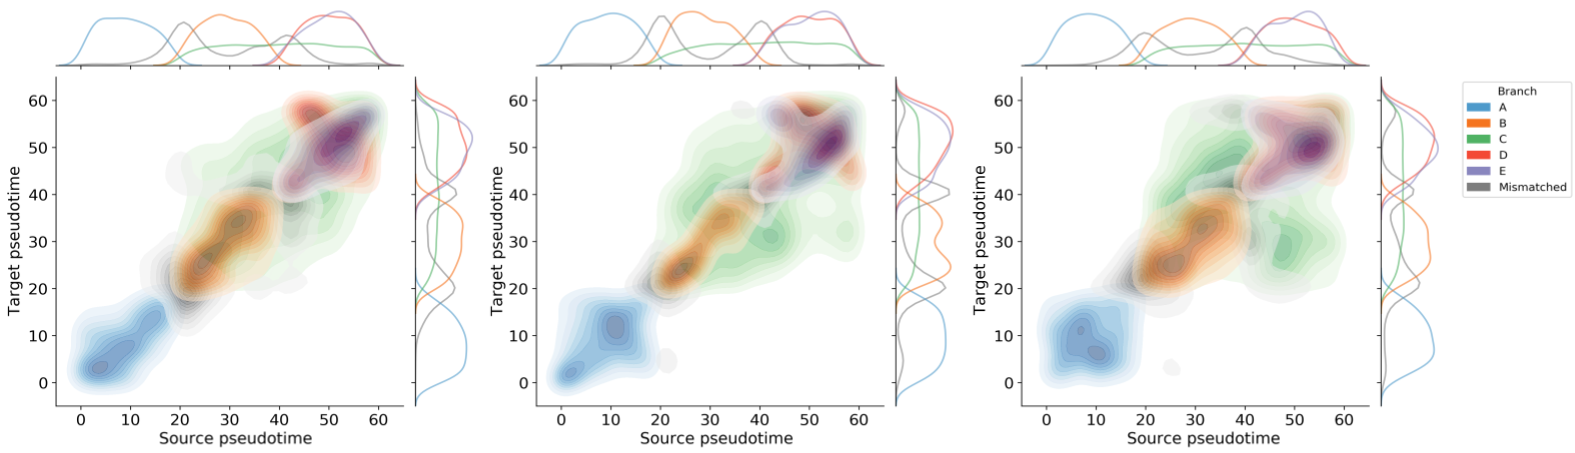
\includegraphics[width=1\textwidth]{figures/integration/3tech-pseudotime-kde.png}
    \caption{
    Evaluation of cross-technology cell matches made by SCIM on the simulated data with three technologies. 
    The pairwise matching is attained for Source-Target A, Source-Target B, and Target A-Target B, respectively. The sink edge capacities were unbounded in all cases.
    Here, we show a density plot for matched pseudotime values between the source technology and the target technology,
    colored by the branch label. Mismatched cells are colored in grey.
    The tree defining the temporal branching process can be found in Figure \ref{fig:prosstt5-pseudotime-inverted}, left.
    Marginal distributions of cell pseudotime for each branch is shown on the top and right.
    }
    \label{fig:prosstt5-3tech-pseudotime}
\end{figure}

\begin{table}
\centering
\begin{tabular}{l|llllll}
\toprule
  method & accuracy & \#null matches & Spearman & Pearson \\
\midrule
 SCIM    &   86\% &  1,590  & 0.83  & 0.86\\
 MATCHER &   4\%  & 25,510  & -0.21 & -0.19\\
\bottomrule
\end{tabular}
\caption{The matching results on the PROSSTT dataset, where the SCIM matching algorithm was applied to SCIM shared latent codes and the MATCHER latent representation. The table depicts accuracy with respect to branch label, null node matches and the correlation coefficients for the pseudotime between matched source and target cells.}
\label{tbl:prosstt_matcher}
\end{table}

\begin{figure}[htp]
    \centering
    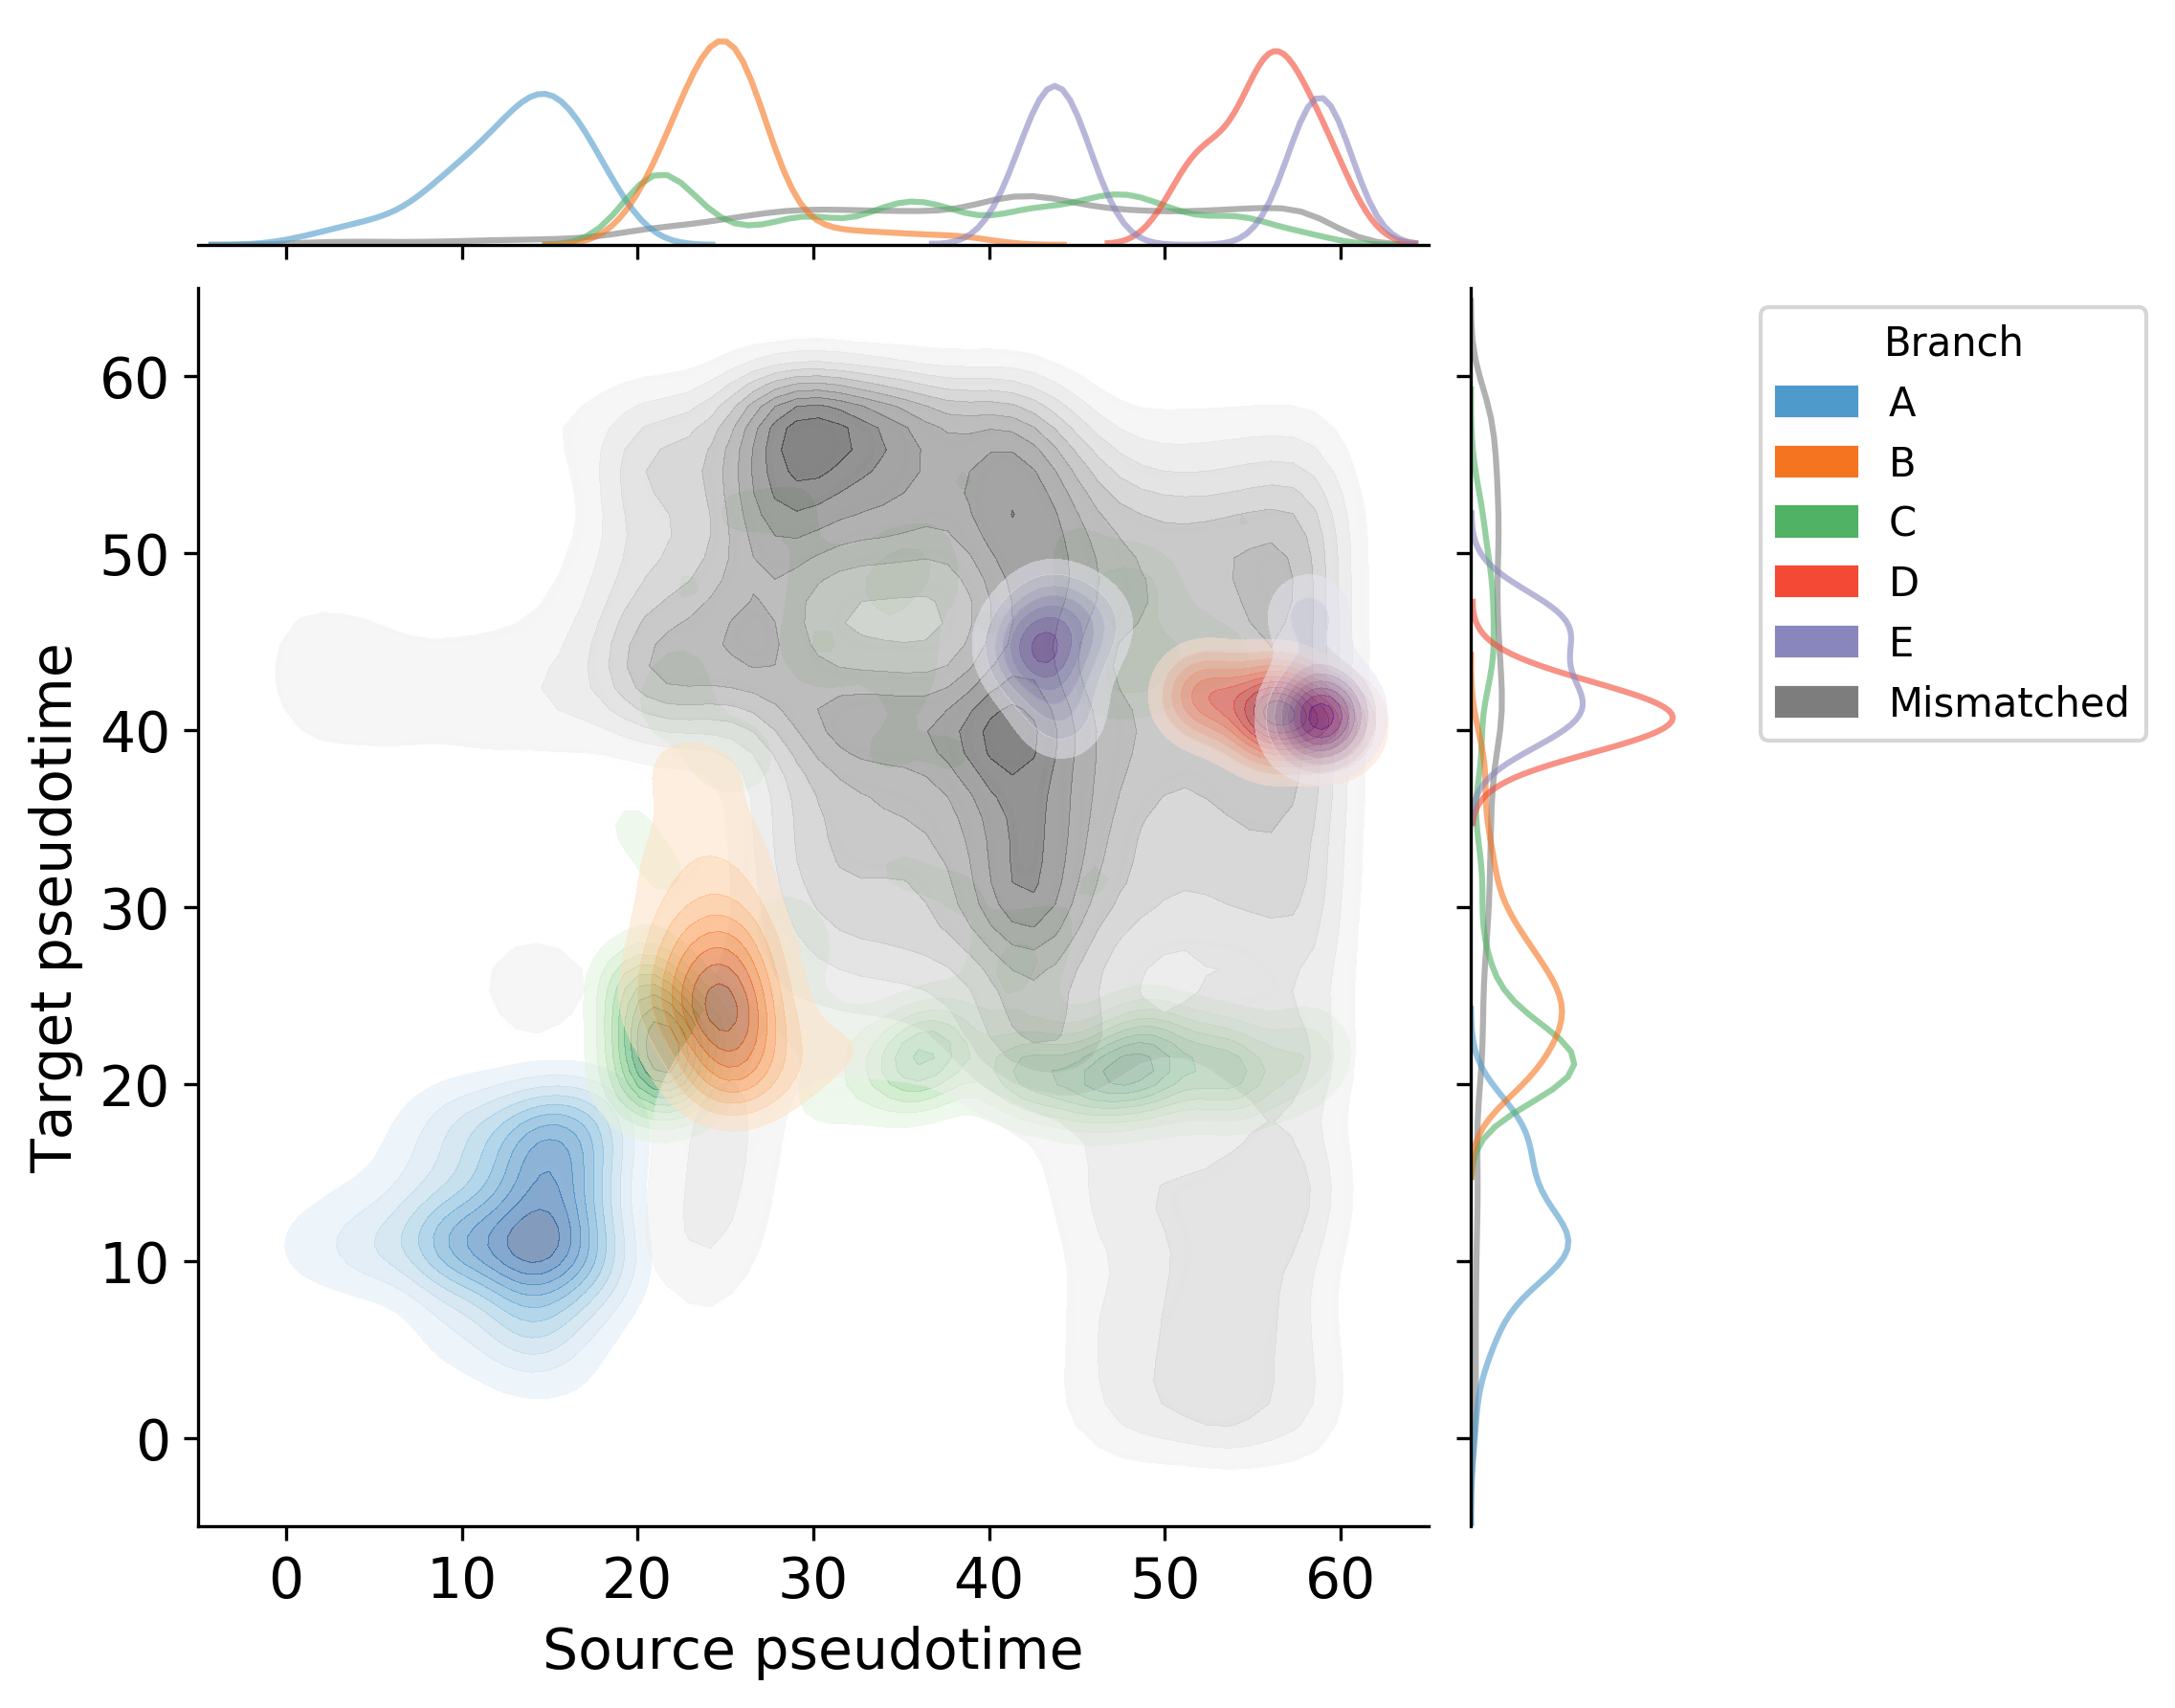
\includegraphics[width=1.0\textwidth]{figures/integration/matcher-pseudotime-kde.png}
    \caption{
    Evaluation of cross-technology cell matches using latent representation obtained by MATCHER on the simulated data.
    Cells are matched across datasets pairwise using the bipartite matching scheme.
    Here we show a density plot for matched pseudotime values between the source technology and the target technology,
    colored by the branch label. Mismatched cells are colored in grey.
    Marginal distributions of cell pseudotime for each branch are shown on the top and right.
    }
    \label{fig:prosstt5-matcher-psuedotime}
\end{figure}

\begin{figure}[htbp]
    \centering
    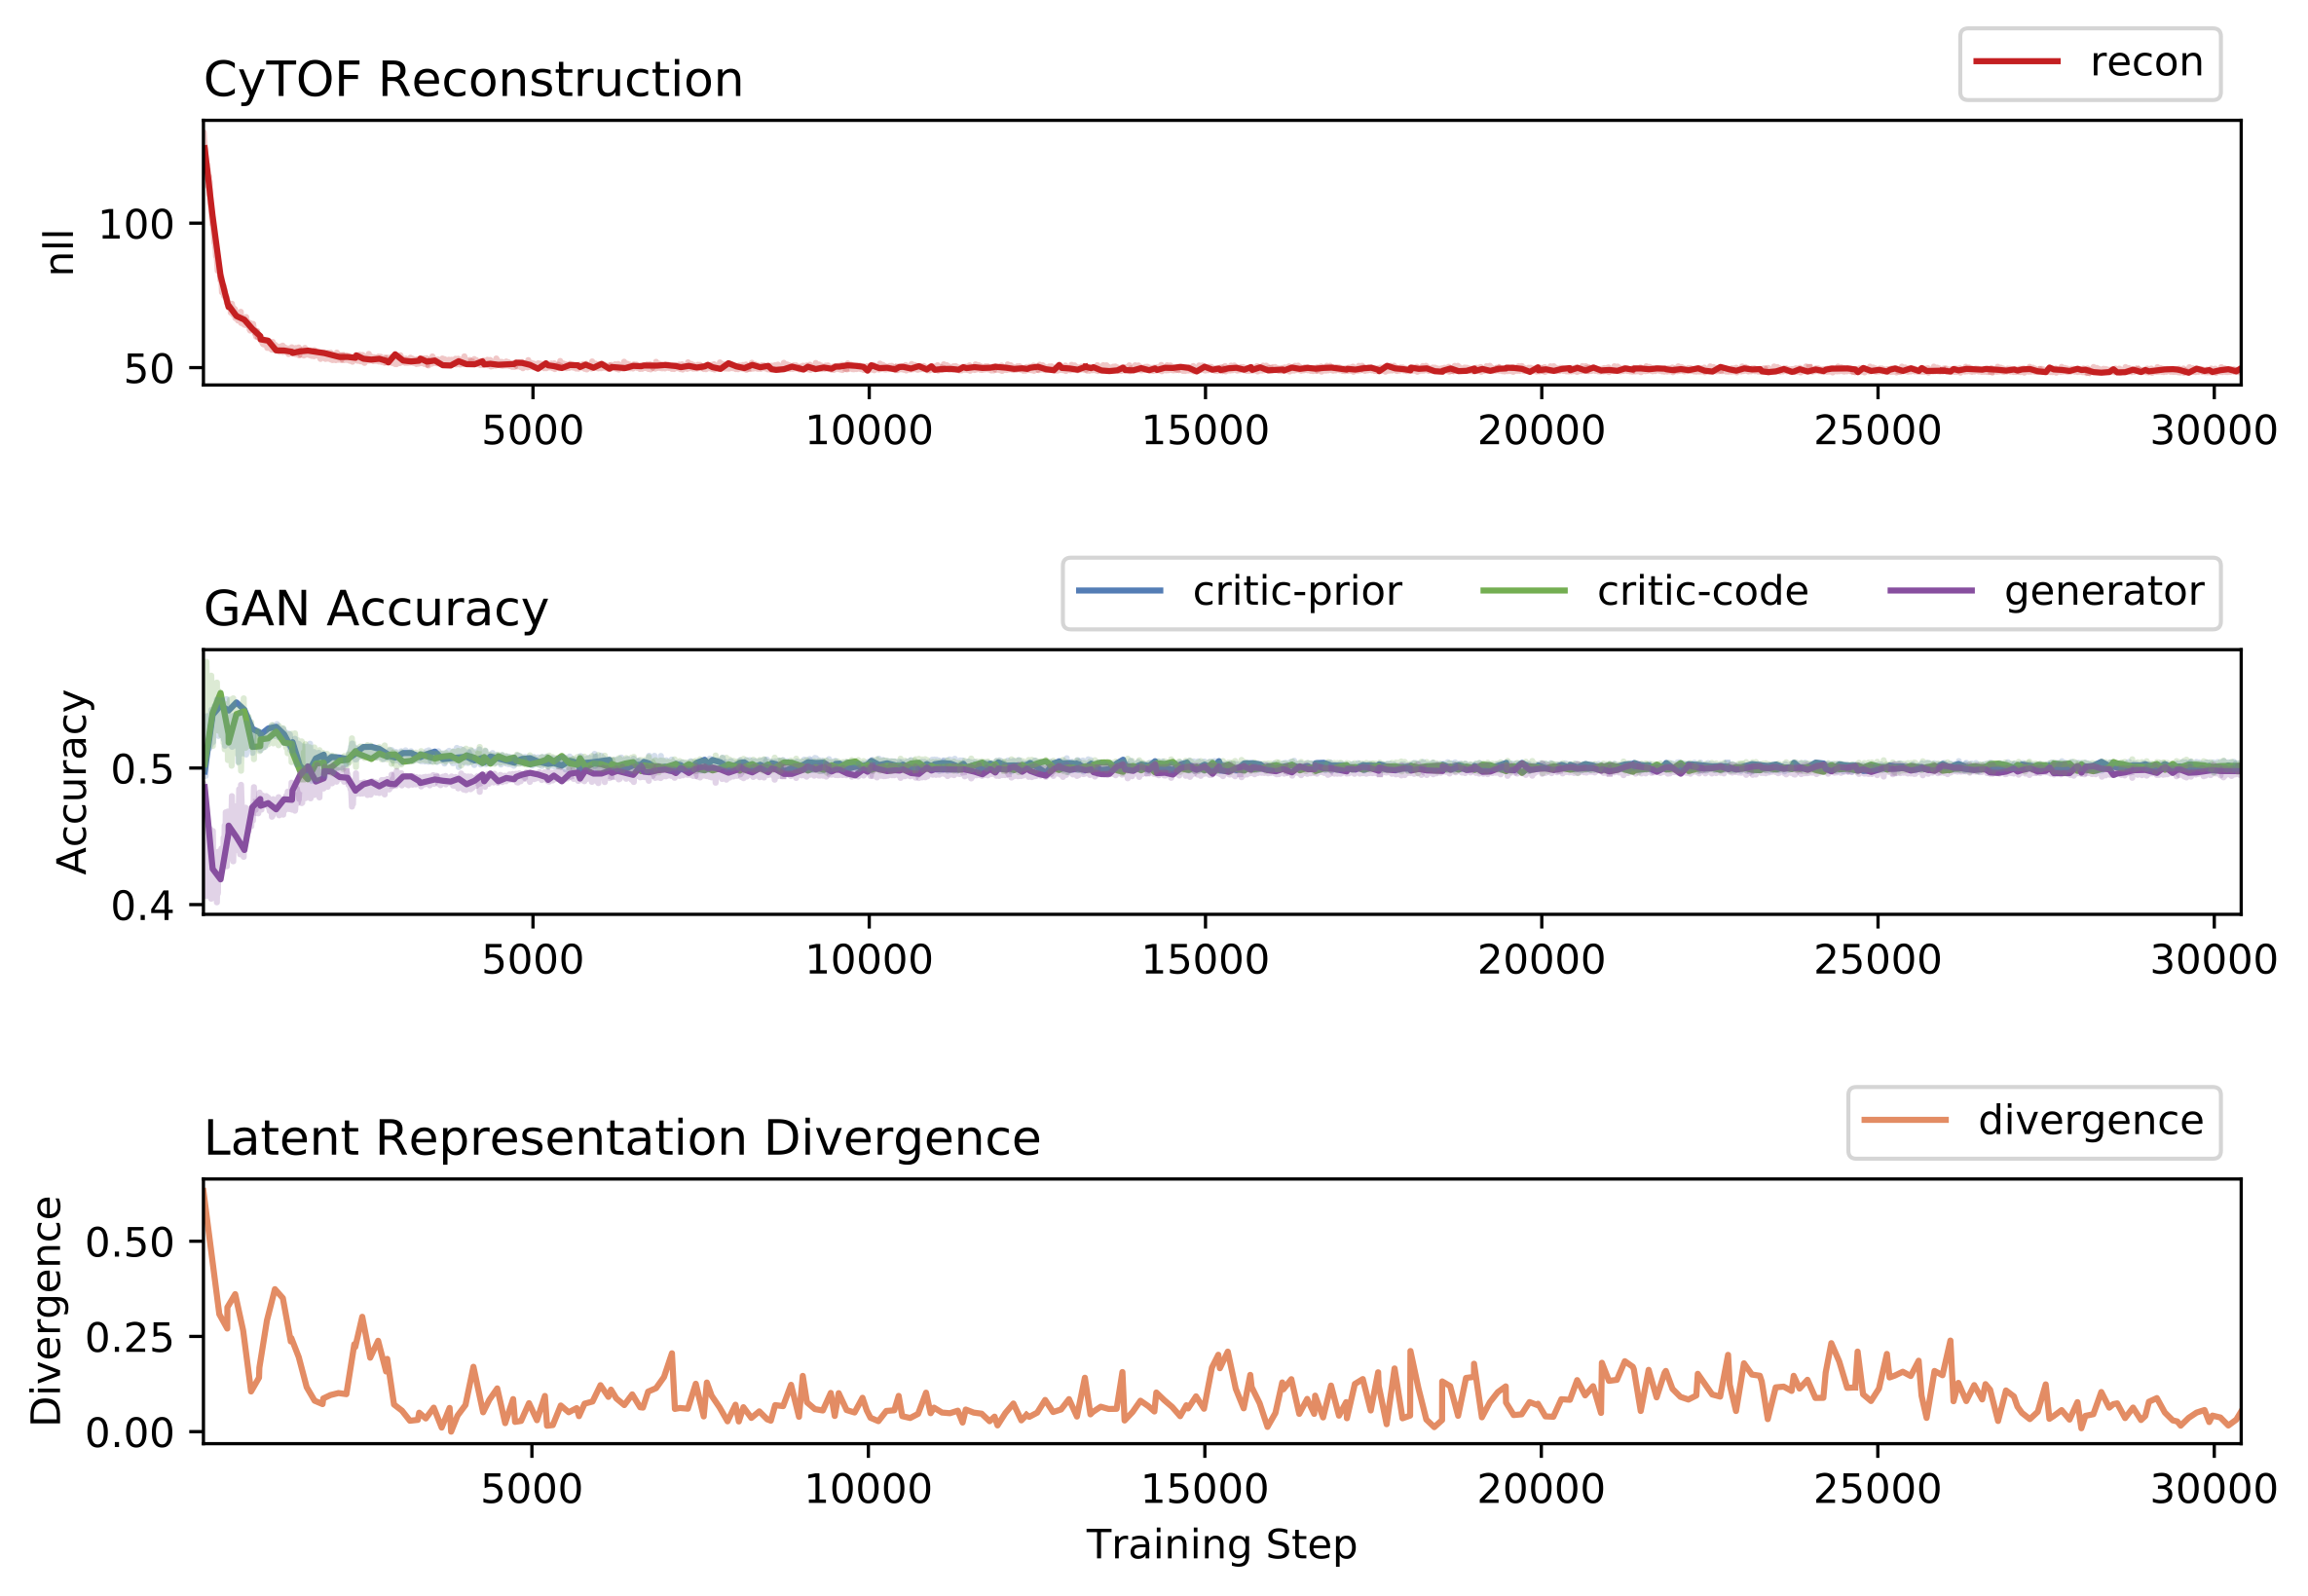
\includegraphics[width=0.95\textwidth]{figures/integration/menytek-train-scores.png}
    \caption{
        Training progress of SCIM on a melanoma sample.
        The latent space is initialized by training a VAE on scRNA data.
        SCIM integrates CyTOF representations into the latent space
        defined by the scRNA codes.
        The top panel shows the negative log-likelihood of the CyTOF reconstruction.
        The middle panel shows the performance of the discriminator to correctly classify scRNA codes (critic-prior), CyTOF codes (critic-code), and the ability of the encoder to fool the discriminator, i.e., the misclassification accuracy (generator).
        The bottom panel shows the divergence of the latent representations.
        The model is able to converge quickly.
However, the divergence score can fluctuate despite still fooling the discriminator.
        Training took 2h 10min and had a peak memory consumption of 1068 MB.
    }
    \label{fig:tupro-train}
\end{figure}


\begin{table}[h]
\centering
\begin{tabular}{rrrrrr}
\toprule
Censor & $\beta$ &  ${lr}_{\phi,\psi}$&  ${lr}_\gamma$ & Success &  \# runs \\
\midrule
0.00 &      16 &            0.0010 &  0.0010 &         14\% &           7 \\
     &      16 &            0.0010 &  0.0005 &         14\% &           7 \\
     &      16 &            0.0005 &  0.0005 &         10\% &          10 \\
     &      16 &            0.0005 &  0.0010 &         10\% &          10 \\
0.25 &      16 &            0.0010 &  0.0010 &         14\% &          14 \\
     &      16 &            0.0005 &  0.0010 &         12\% &          17 \\
     &      64 &            0.0001 &  0.0005 &          0\% &           7 \\
     &      64 &            0.0001 &  0.0010 &          0\% &           7 \\
0.75 &      16 &            0.0005 &  0.0010 &         17\% &           6 \\
     &      32 &            0.0005 &  0.0005 &         12\% &           8 \\
     &      16 &            0.0010 &  0.0005 &          8\% &          13 \\
     &      64 &            0.0001 &  0.0005 &          0\% &           7 \\
0.90 &      16 &            0.0005 &  0.0010 &         40\% &          10 \\
     &      16 &            0.0010 &  0.0005 &         10\% &          10 \\
     &      16 &            0.0005 &  0.0005 &          8\% &          12 \\
     &      32 &            0.0010 &  0.0001 &          0\% &          10 \\
0.95 &      32 &            0.0010 &  0.0001 &          0\% &           4 \\
     &      64 &            0.0001 &  0.0005 &          0\% &           4 \\
     &      64 &            0.0001 &  0.0010 &          0\% &           6 \\
     &      32 &            0.0010 &  0.0010 &          0\% &           5 \\
0.99 &      16 &            0.0005 &  0.0010 &         17\% &           6 \\
     &      32 &            0.0010 &  0.0005 &          0\% &           6 \\
     &      64 &            0.0001 &  0.0005 &          0\% &           4 \\
     &      32 &            0.0010 &  0.0001 &          0\% &           6 \\
\bottomrule
\end{tabular}
\caption{
    Ablation study for training SCIM on the melanoma patient at several levels of semi-supervision.
    Fraction censored is the fraction of labels removed during training.
    The top 4 configurations for each level of semi-supervision is shown.
    $\beta$ is the regularization strength of the adversarial loss.
    Learning rates are the initial settings of the ADAM optimizer.
    If the latent space divergence is below 0.3 and
    the negative log-likelihood of the input under the reconstruction is below 47,
    the training is determined to be a success. These values were chosen empirically.
    We see that $\beta$ and optimizer learning rates were heavily influential on model success.
}
\label{tbl:ablation_menytek}
\end{table}

\begin{figure}[h]
    \centering
    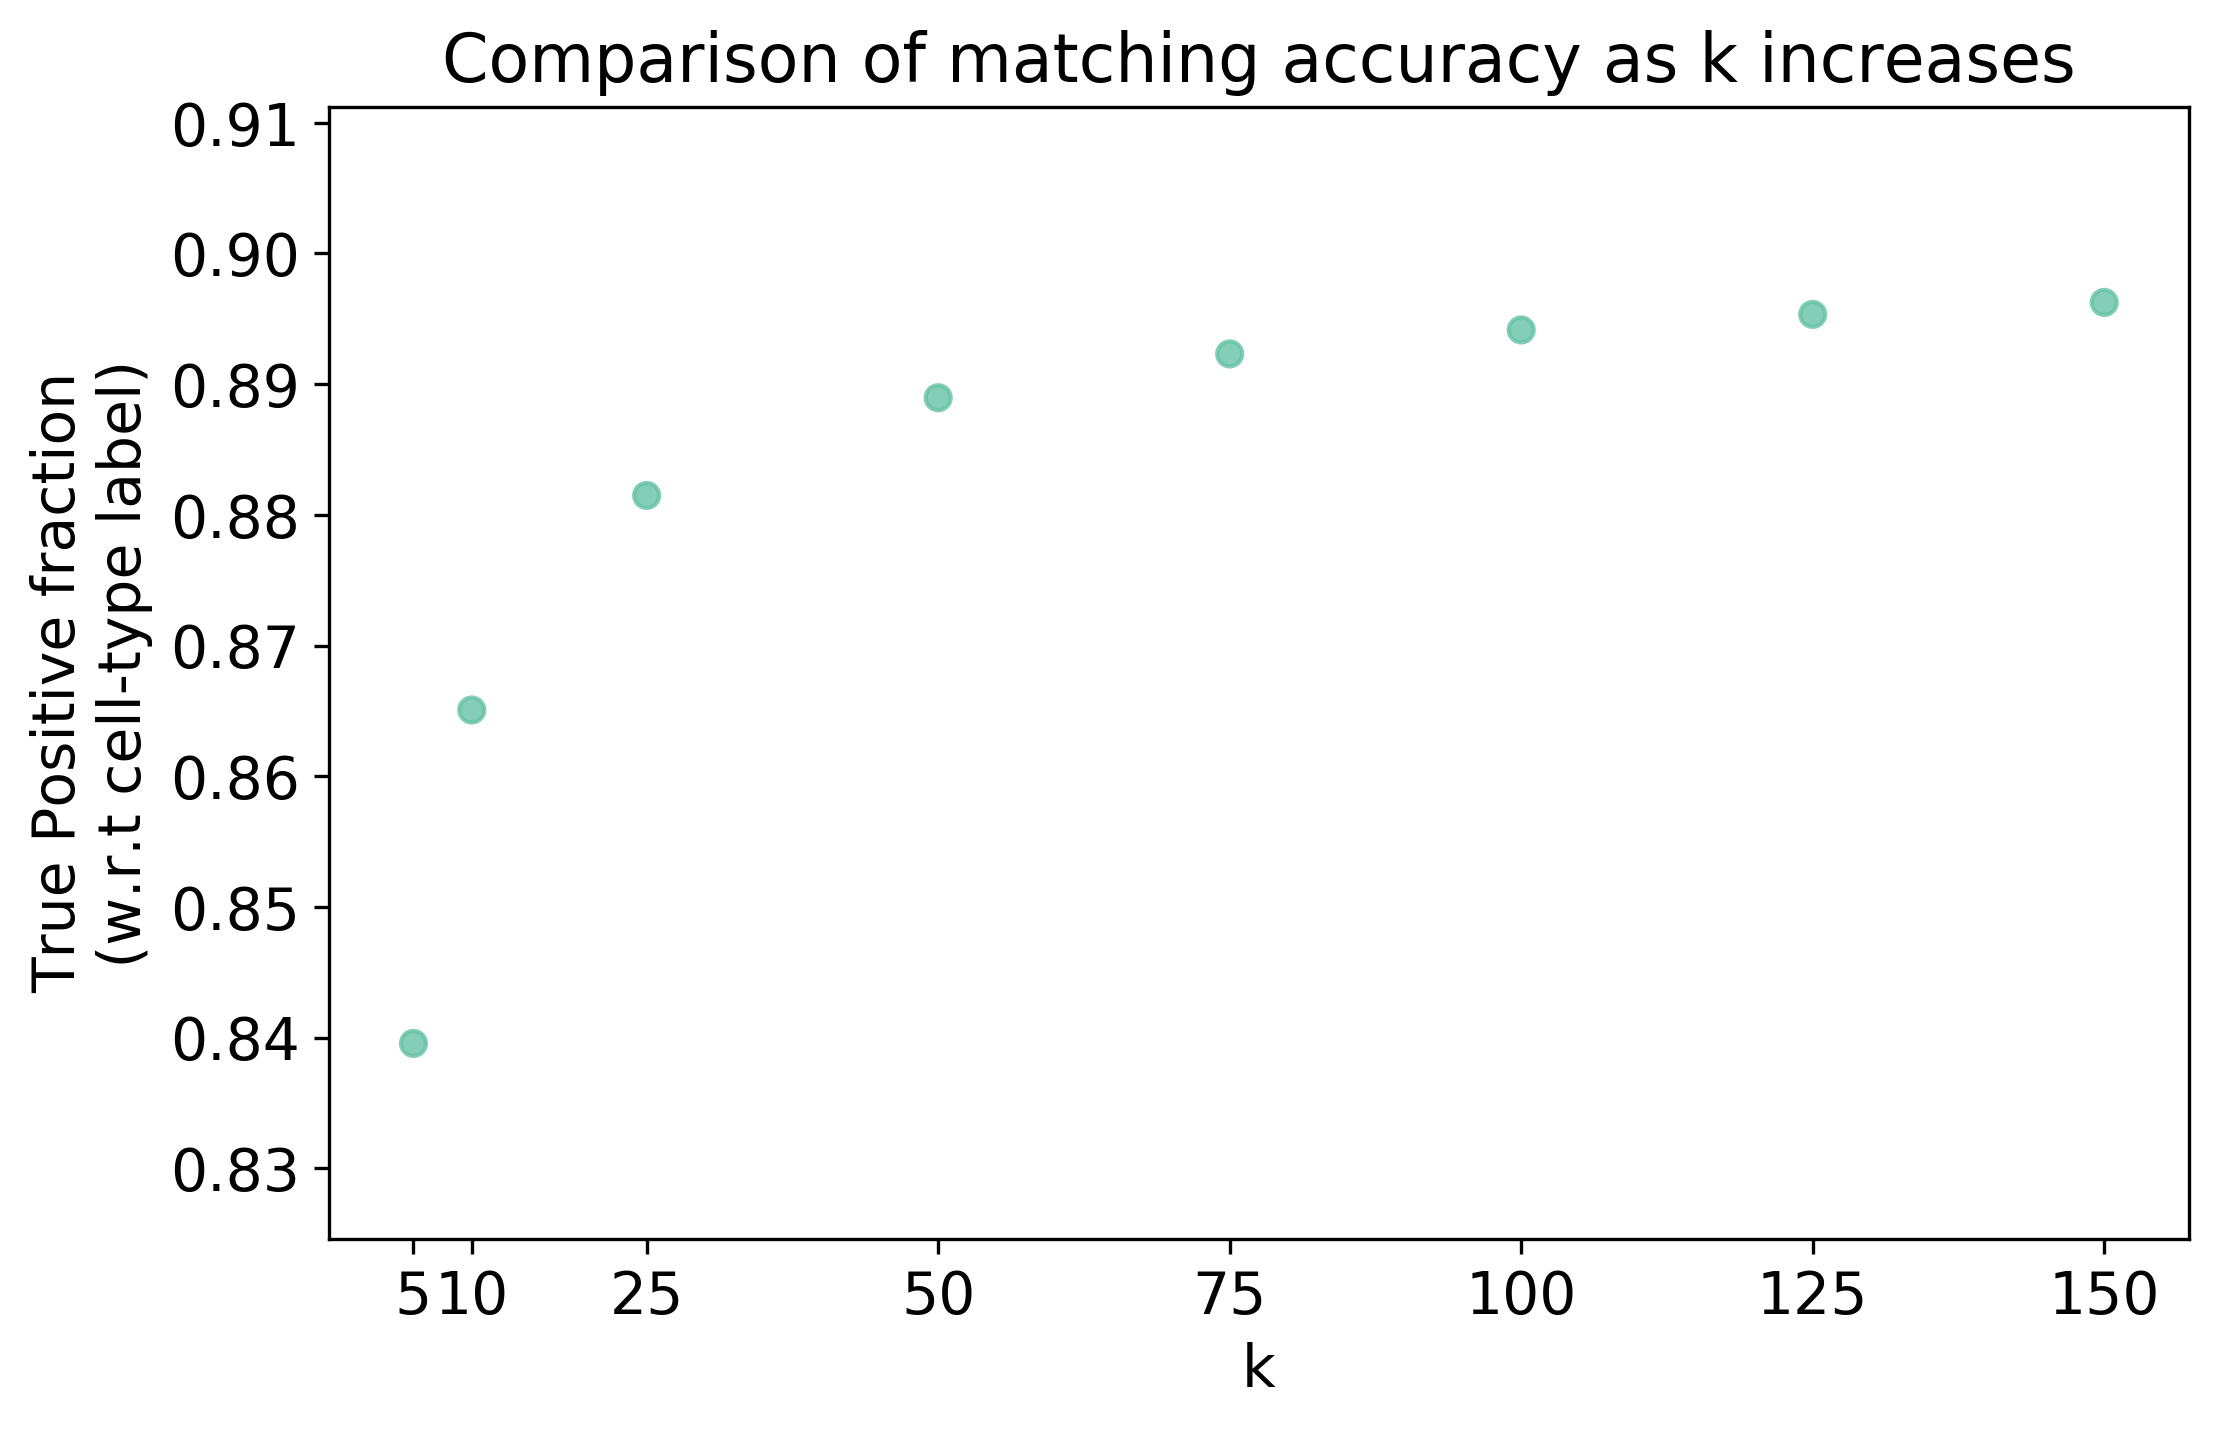
\includegraphics[width=0.85\textwidth]{figures/integration/matching-tune-k-unicapacity.png}
    \caption{Comparison of matching accuracy, with respect to cell-type label as less sparsity of connections, is imposed on the Tumor Profiler data.
The number of considered Nearest Neighbors \textit{k} is indicated on the x-axis, and the fraction of true positive matches, with respect to cell-type label, is depicted on the y-axis.
 The accuracy level saturates with $k=100$.}
    \label{fig:matching_accuracy_log10_uni}
\end{figure}

\begin{table}[h]
\centering
\begin{tabular}{lrr}
\toprule
{} &  CPU time [s] &  Max Memory [Mb] \\
k   &               &                  \\
\midrule
5   &       1,492.67 &          1,674.94 \\
10  &       2,803.33 &          2,456.27 \\
25  &       7,723.67 &          4,690.05 \\
50  &       7,441.33 &          8,740.34 \\
75  &      12,656.00 &         12,344.52 \\
100 &      17,331.00 &         17,002.75 \\
125 &      26,047.00 &         20,612.78 \\
150 &      33,718.00 &         24,222.75 \\
\bottomrule
\end{tabular}
\caption{Memory usage and computation time of the bipartite matching as \textit{k} hyperparameter in kNN search increases.
The values were obtained on the whole TuPro dataset using the MCMF algorithm on an extended graph. %, as described in section \ref{graph_extensions}.
The cost of matching to the null node was set to 95th percentile, and a union of connections obtained from kNN graphs with \textit{k} indicated in the first column was used for matching.
The memory and time reports were averaged across three independent runs.}
\label{tbl:menytek_tune_k_uni}
\end{table}

\begin{figure}[htbp]
    \centering
    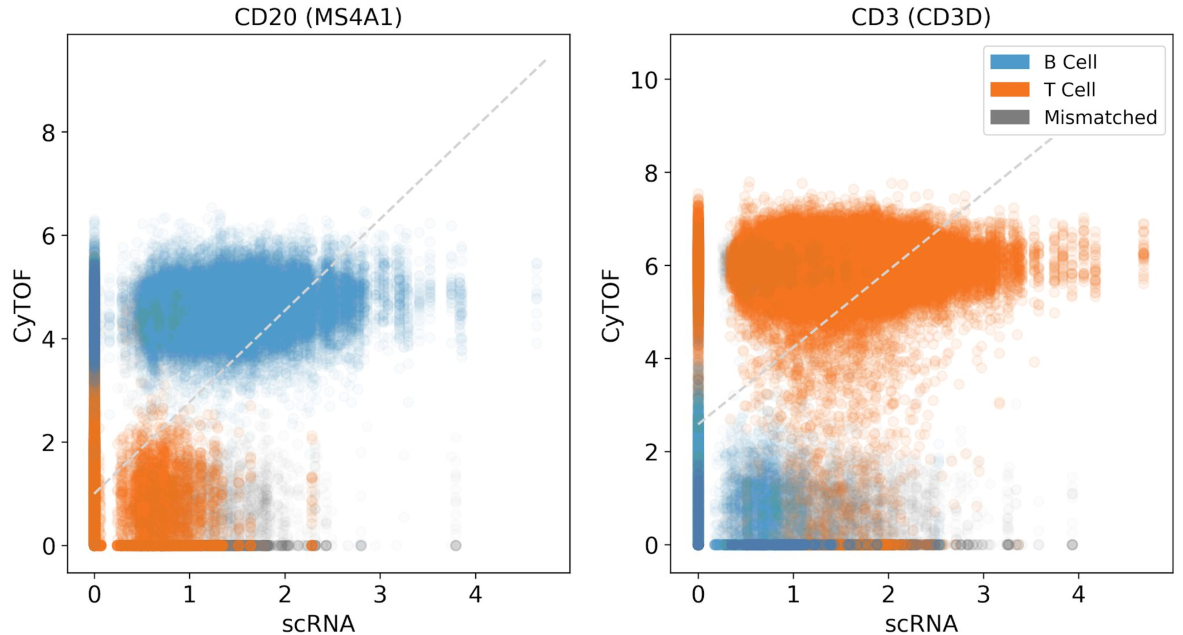
\includegraphics[width=0.65\textwidth]{figures/integration/gene_protein_correlation_unicapacity.pdf}
    \caption{
      \textit{CD20} and \textit{CD3} marker abundances measured with scRNA (gene, x-axis) and CyTOF (protein, y-axis) in a melanoma sample from the Tumor Profiler Consortium.
      The values on the axes represent normalized expression.
      Colors (blue, orange) represent cell types (B-cell, T-cell) while grey marks mismatches with respect to the cell-type label.
      The linear regression line is depicted by a dashed light grey line.
      Pearson's correlation coefficient equals 0.63 and 0.51 for CD20 and CD3, respectively.
      Spearman's correlation coefficient amounts to 0.55 and 0.42, for CD20 and CD3, respectively.
    }
    \label{fig:tupro-marker-correlation-uni}
\end{figure}

\begin{figure}[htb]
    \centering
    \includegraphics[width=0.85\textwidth]{figures/integration/oetjen-tsne-matched-unicapacity.png}
    \caption{
    A tSNE embedding (perplexity=30) of the integrated latent space with cell matches indicated by the grey lines.
    The shared representation was obtained in a semi-supervised fashion, utilizing 10\% of the cell-type labels to orient the latent space. 10,000 matched pairs were sampled at random for the plot.
    Colors (blue, green, orange) represent T-cell subtypes (CD8 effector, CD4 naive, CD4 memory), and color shades correspond to the profiling technology (light: scRNA, dark: CyTOF).}
    \label{fig:oetjen_tsne_uni}
\end{figure}

\cleardoublepageempty{}

\section{Learning to align single-cell perturbation responses}
\begin{figure}[H]
    \centering
    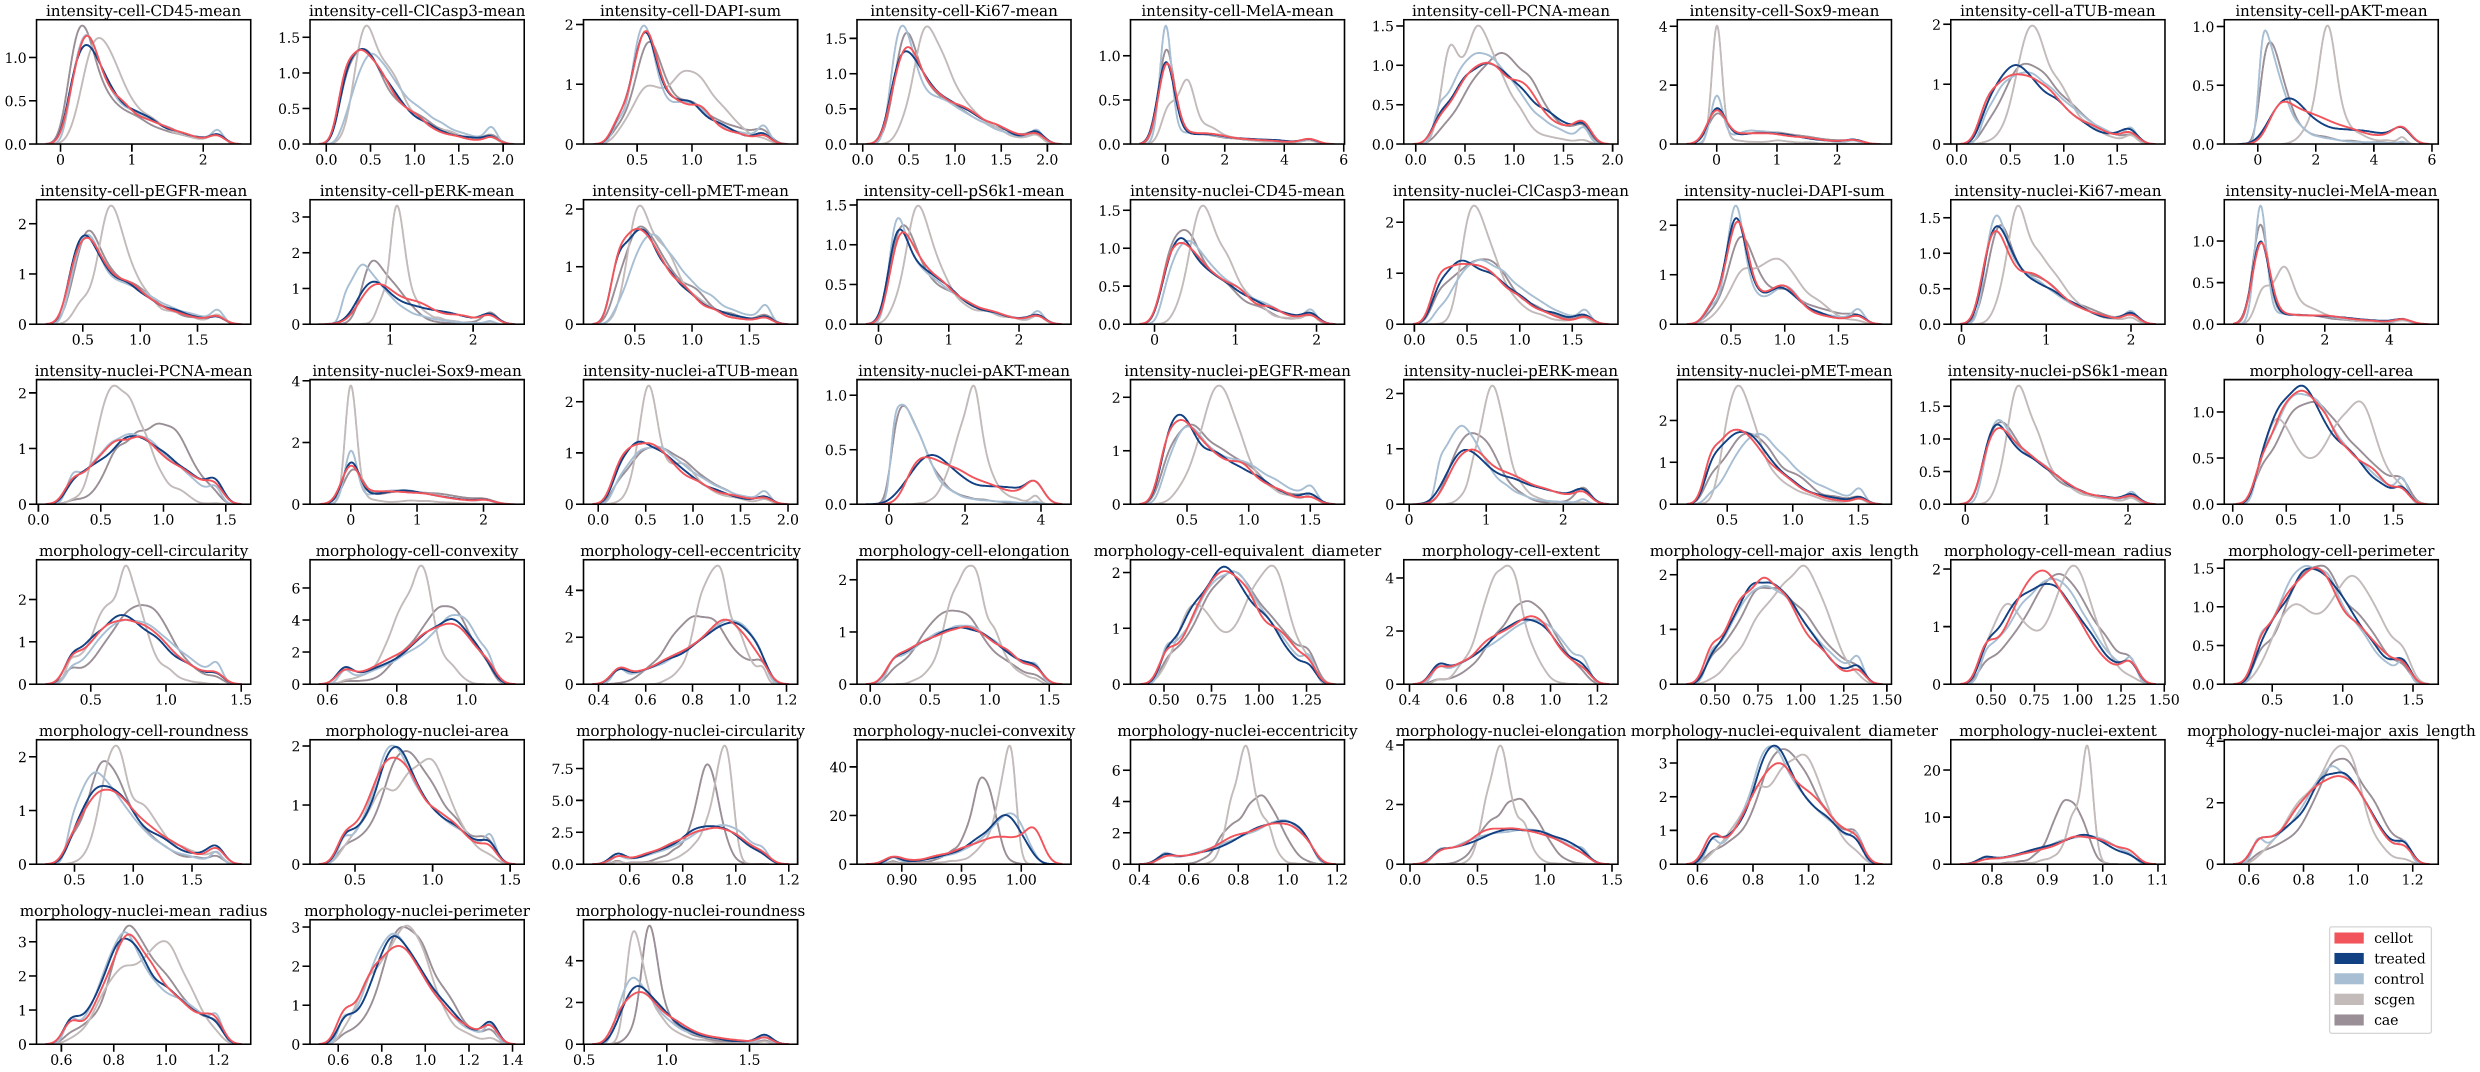
\includegraphics[width=\textwidth]{figures/cellot-methods/Bunne_Supp_Fig1.png}
    \caption{Predicted and observed marginals of cells profiled by 4i, treated with Imatinib. All extracted intensity and morphology features are shown.}
    \label{supp_fig:4i_all_marginals_imatinib}
\end{figure}

\begin{figure}[H]
    \centering
    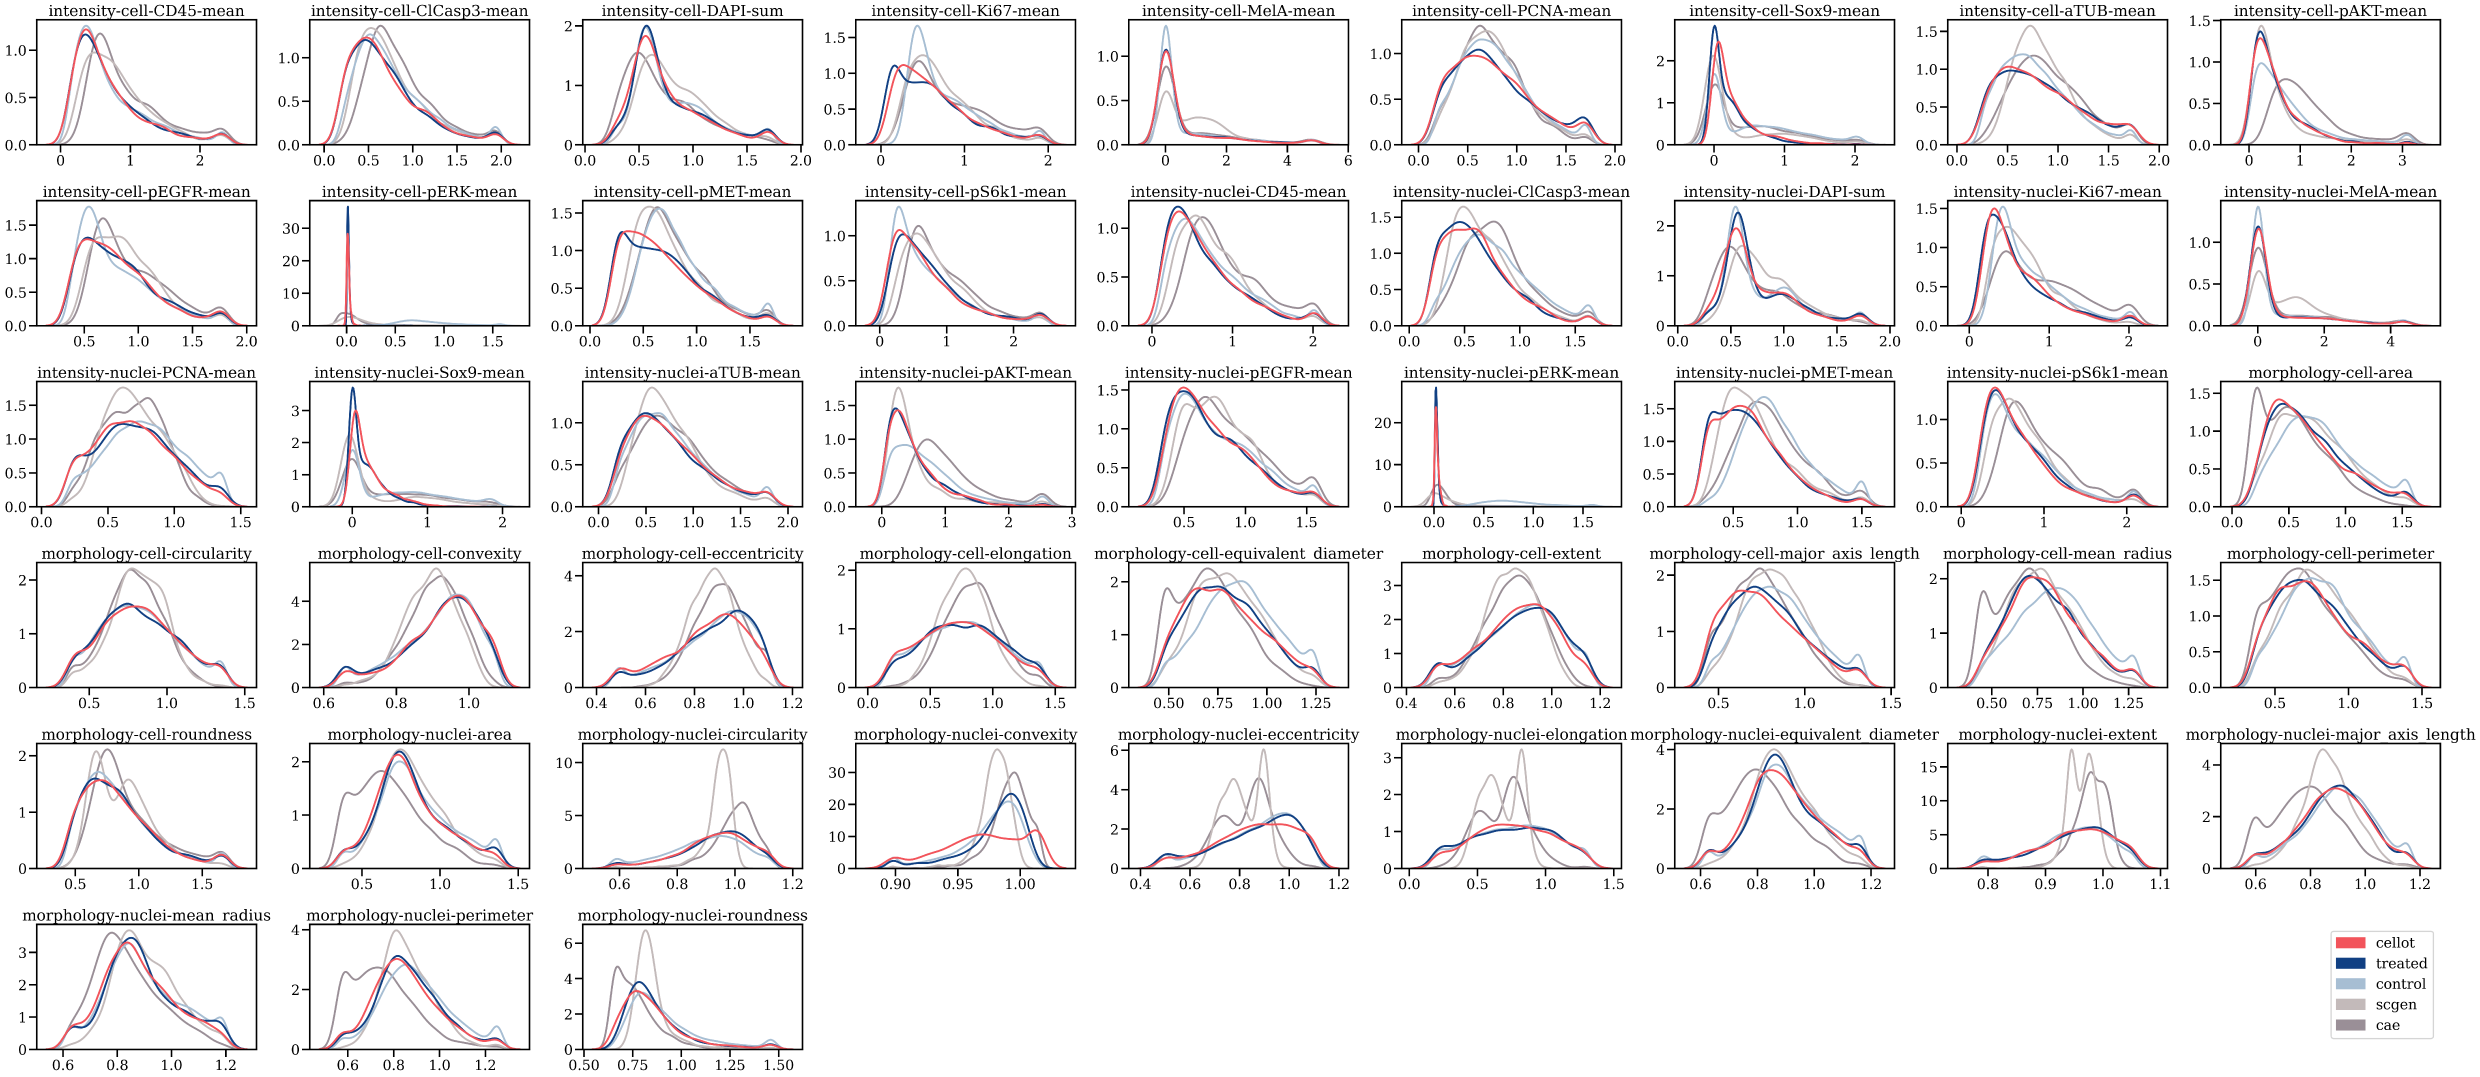
\includegraphics[width=\textwidth]{figures/cellot-methods/Bunne_Supp_Fig2.png}
    \caption{Predicted and observed marginals of cells profiled by 4i treated with Trametinib. All extracted intensity and morphology features are shown.}
    \label{supp_fig:4i_all_marginals_trametinib}
 \end{figure}
 
 \begin{figure}[H]
    \centering
    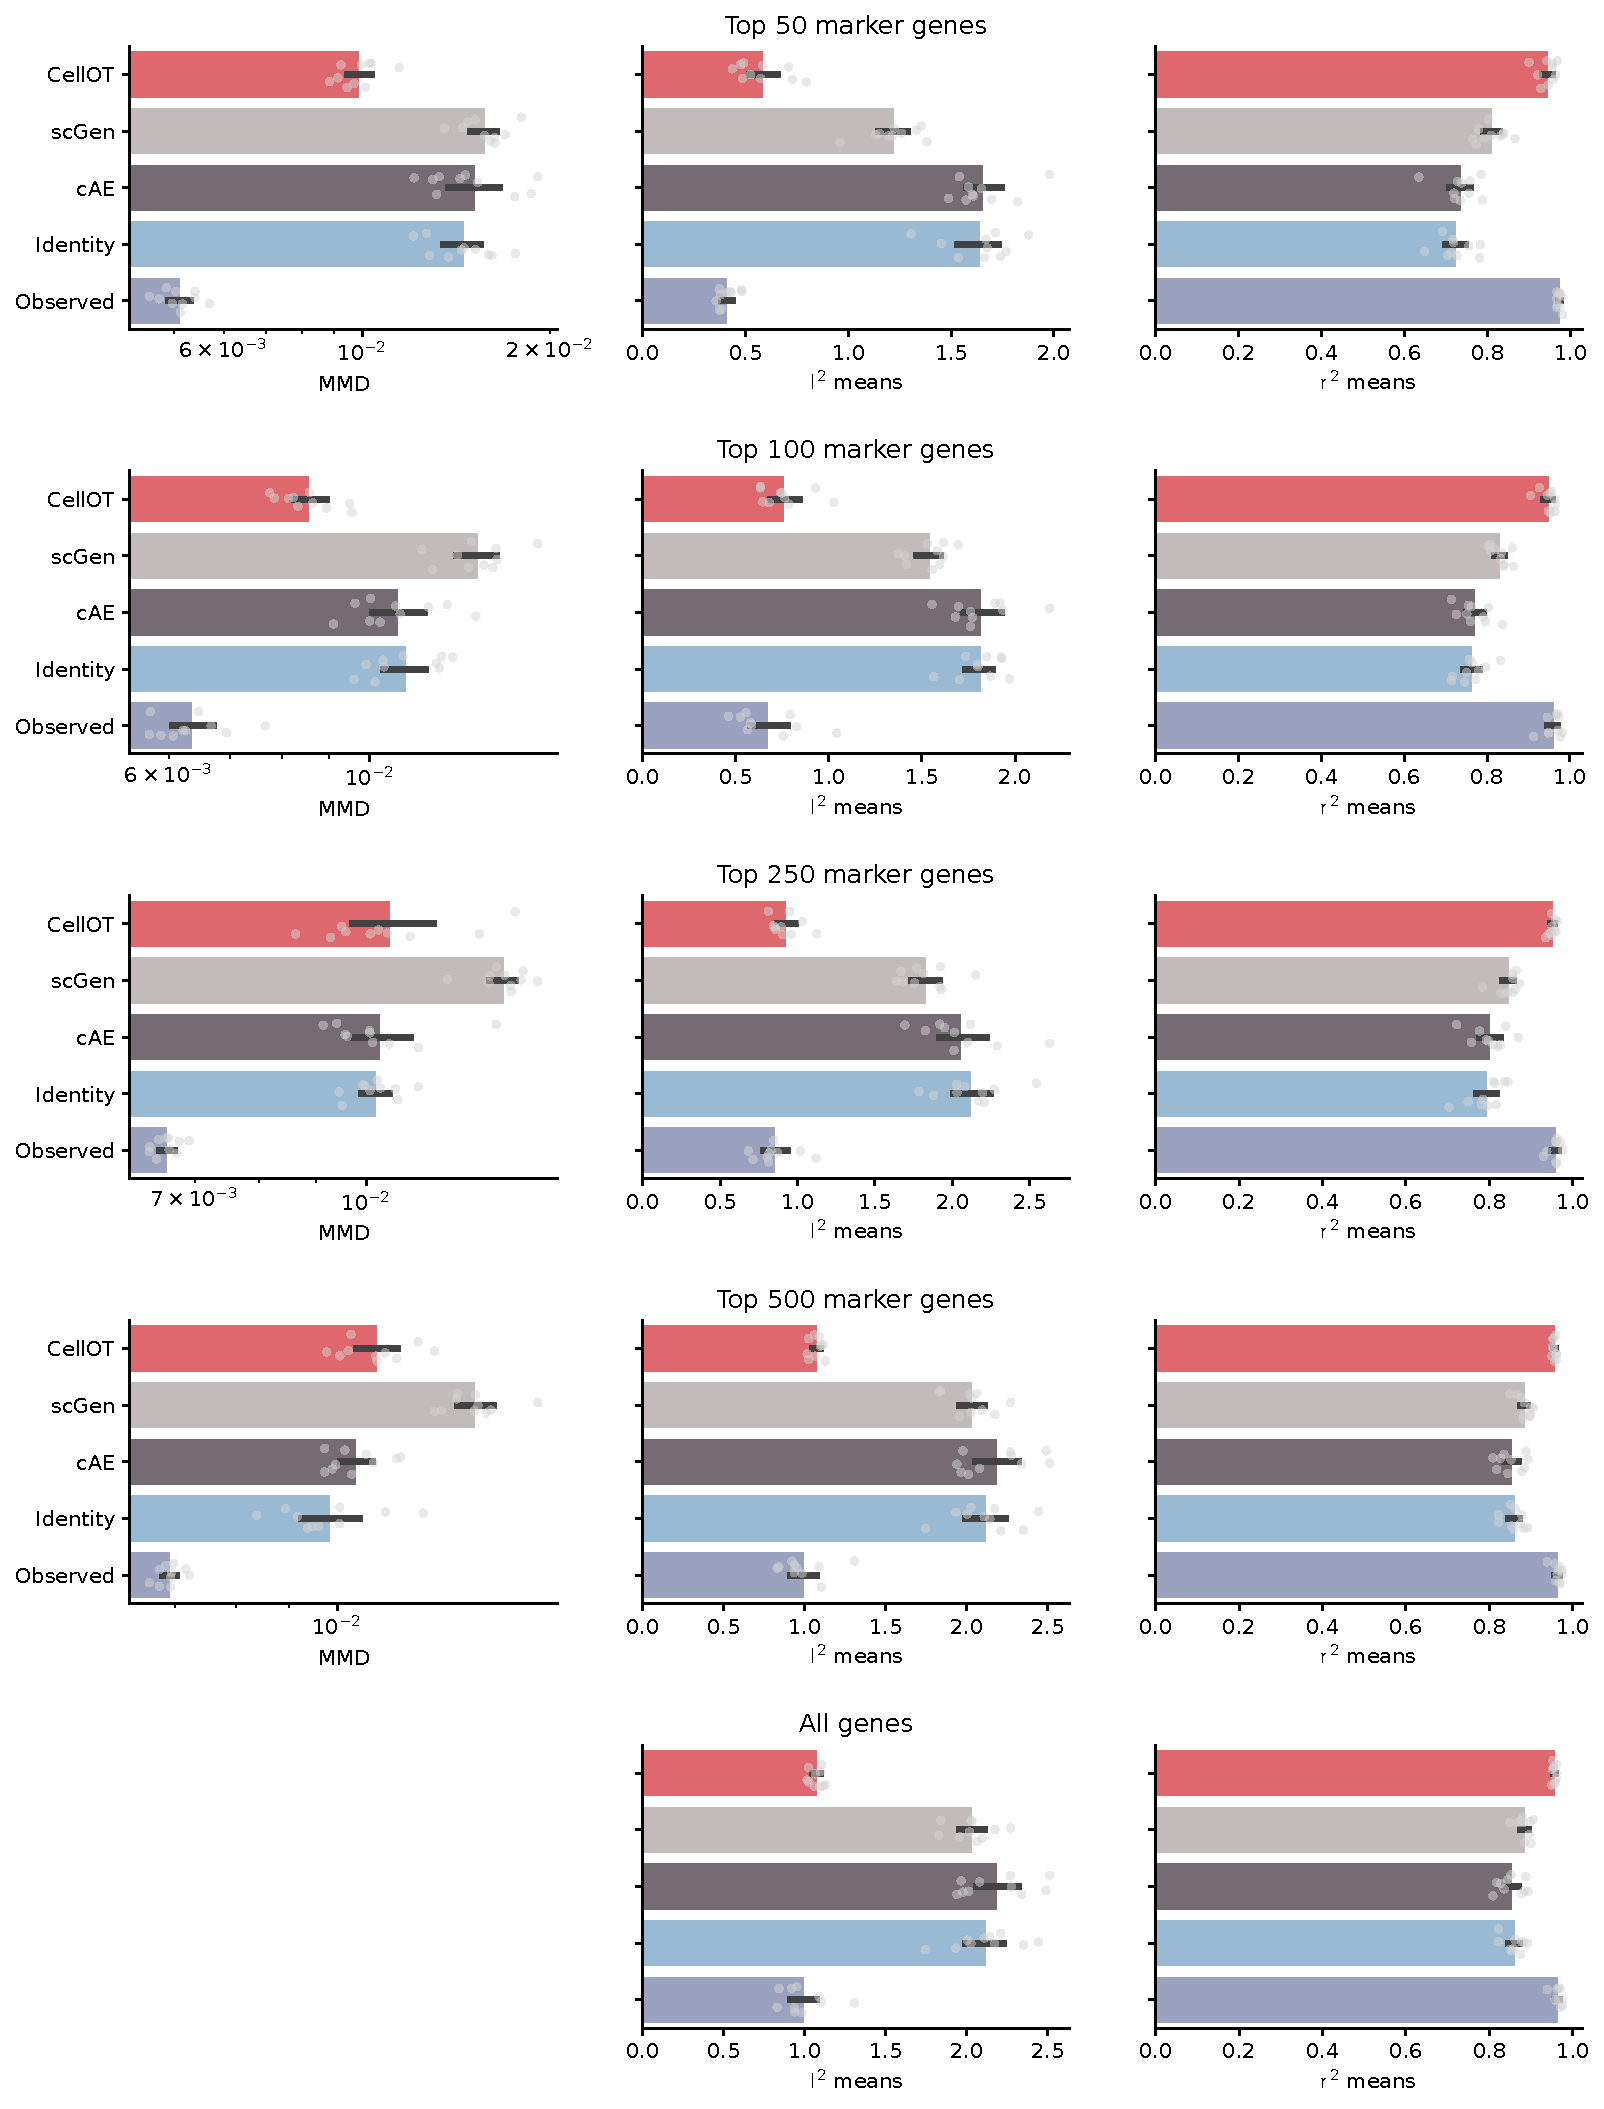
\includegraphics[width=0.9\textwidth]{figures/cellot-methods/Bunne_Supp_Fig7.pdf}
    \caption{Results for single-cell responses for Trametinib the SciPlex3 dataset for different metrics computed on 50, 100, 250, and 500 marker genes, including MMD, $\ell_2$ feature means, and $r^2$ correlation feature means for \textsc{CellOT} as well as different baselines. With increasing dimensionality, the MMD computation is biased. Data is presented as the mean +/- standard deviation across n=10 bootstraps of the test set.}
    \label{supp_fig:sciplex_num_markers}
\end{figure}

\begin{figure}[H]
    \centering
    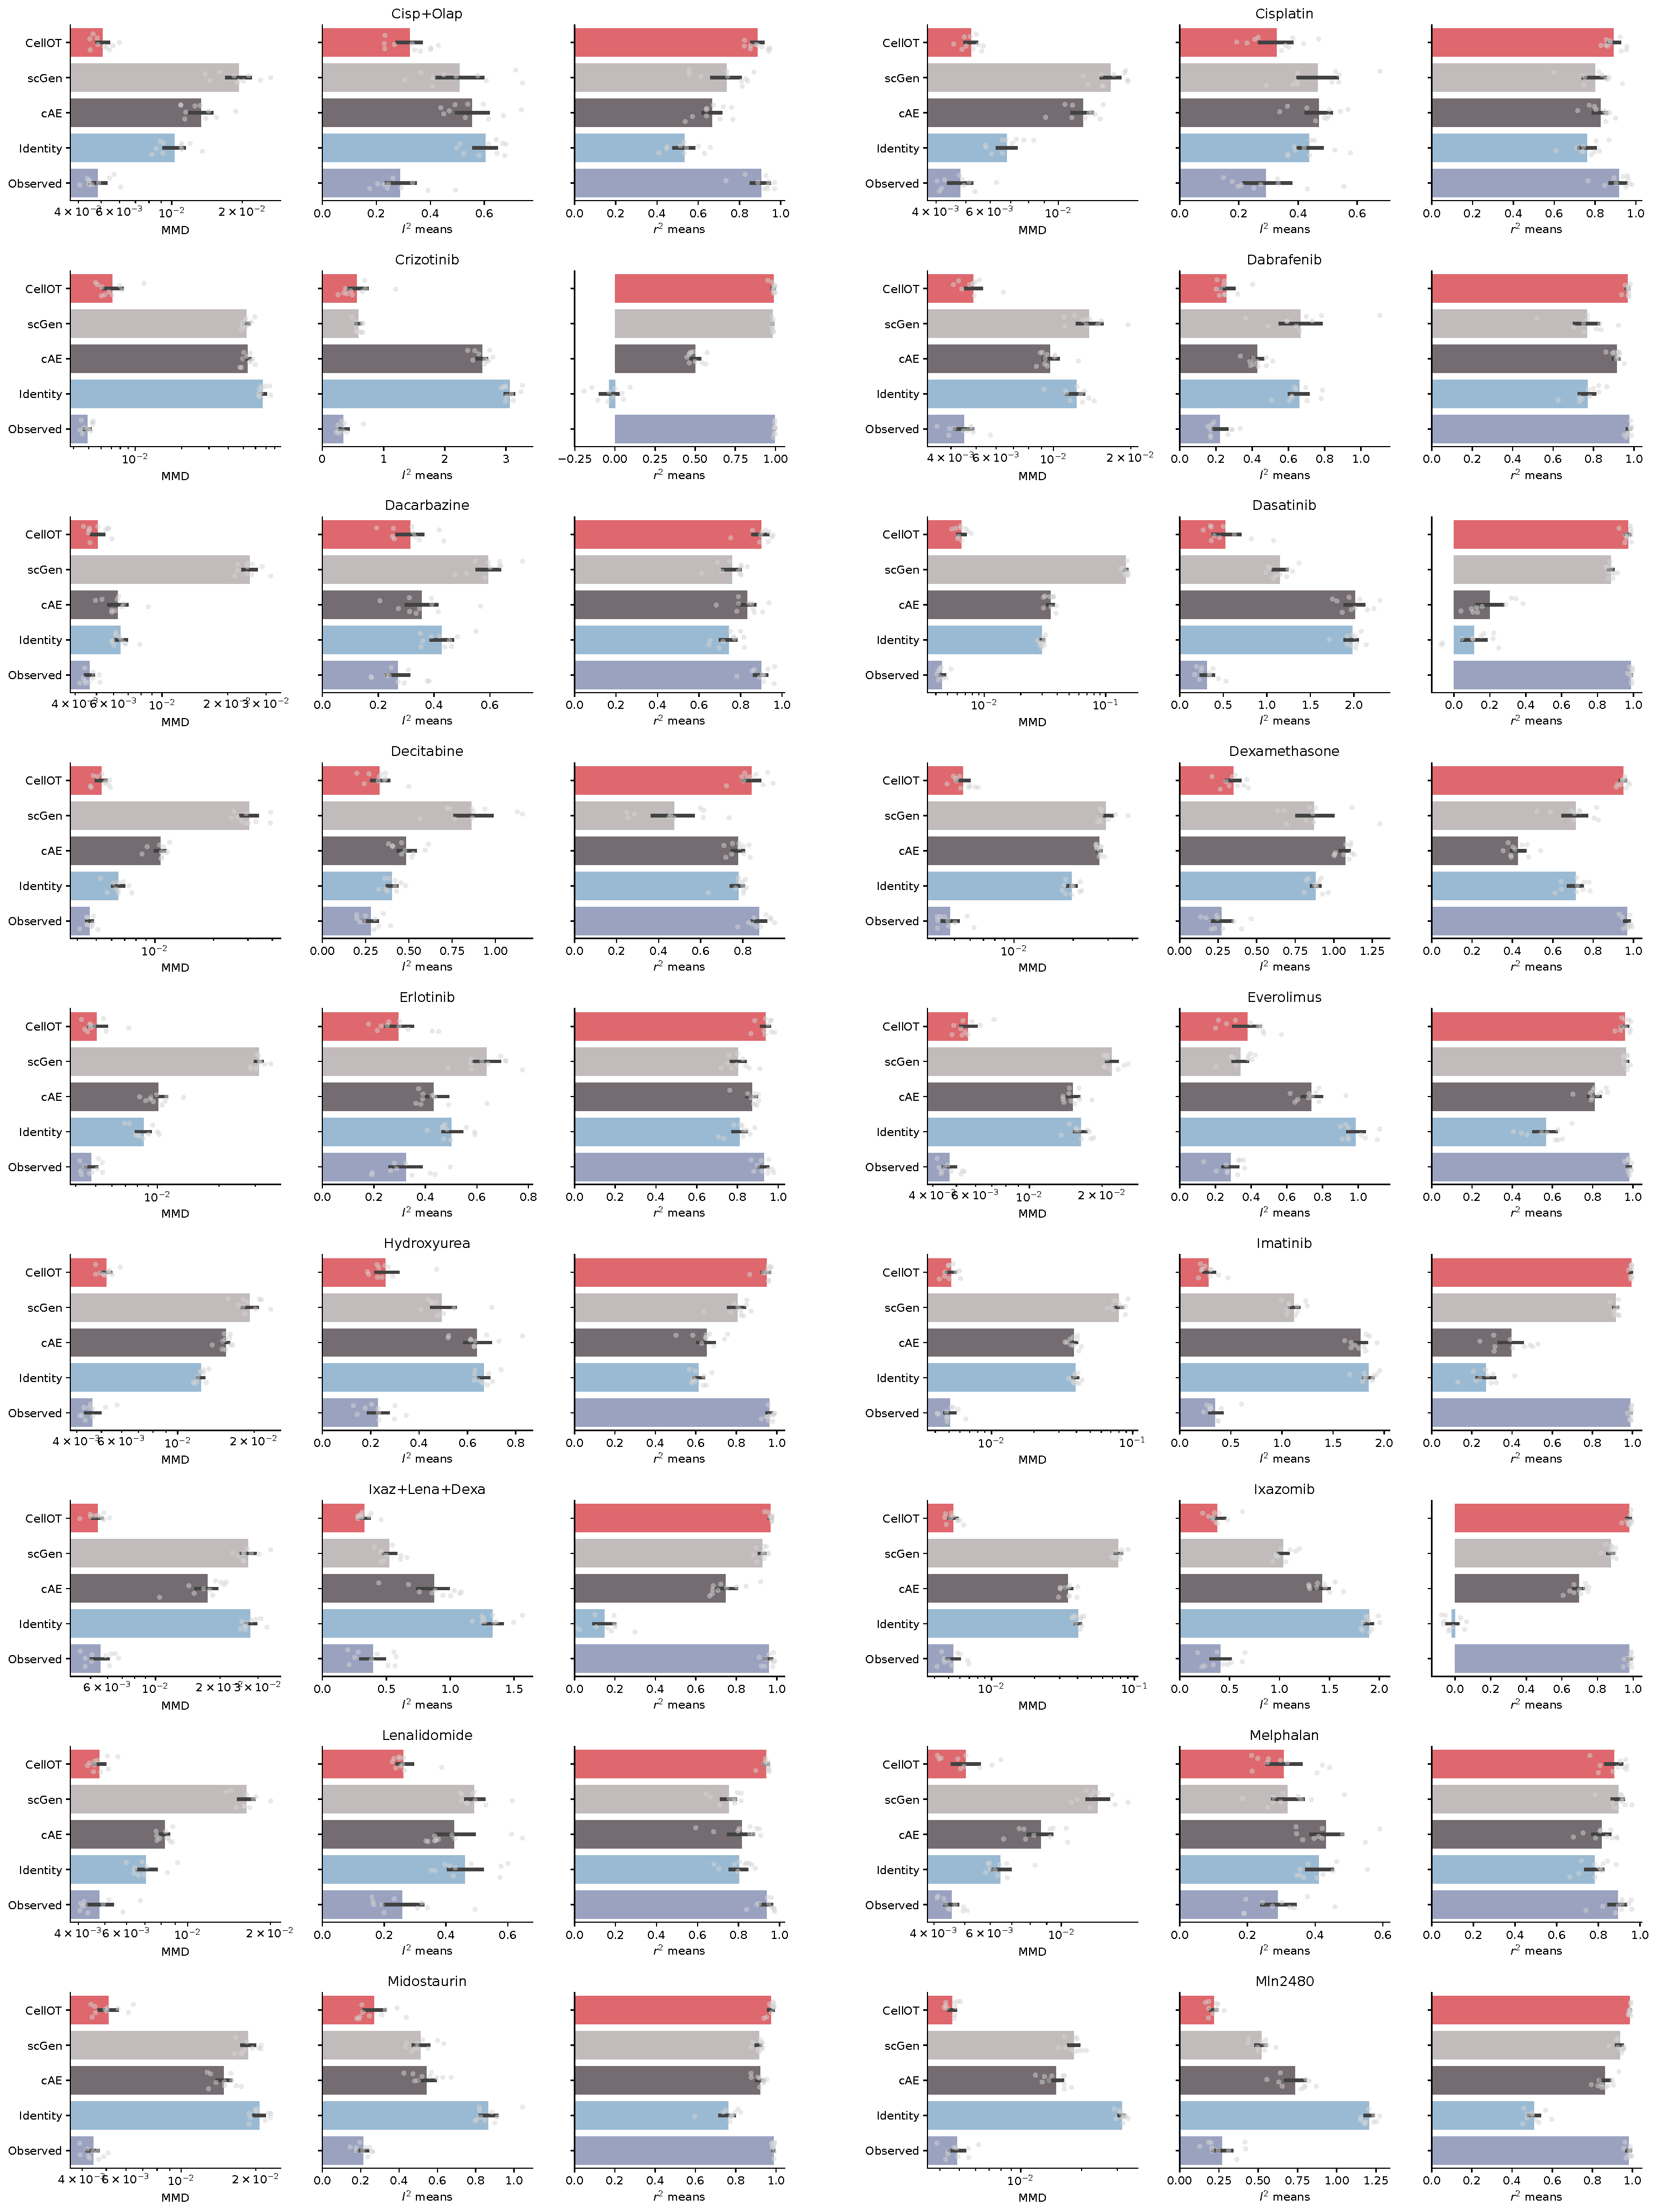
\includegraphics[width=\textwidth]{figures/cellot-methods/Bunne_Supp_Fig5_p1.pdf}
\end{figure}
\begin{figure}[H]
    \centering
    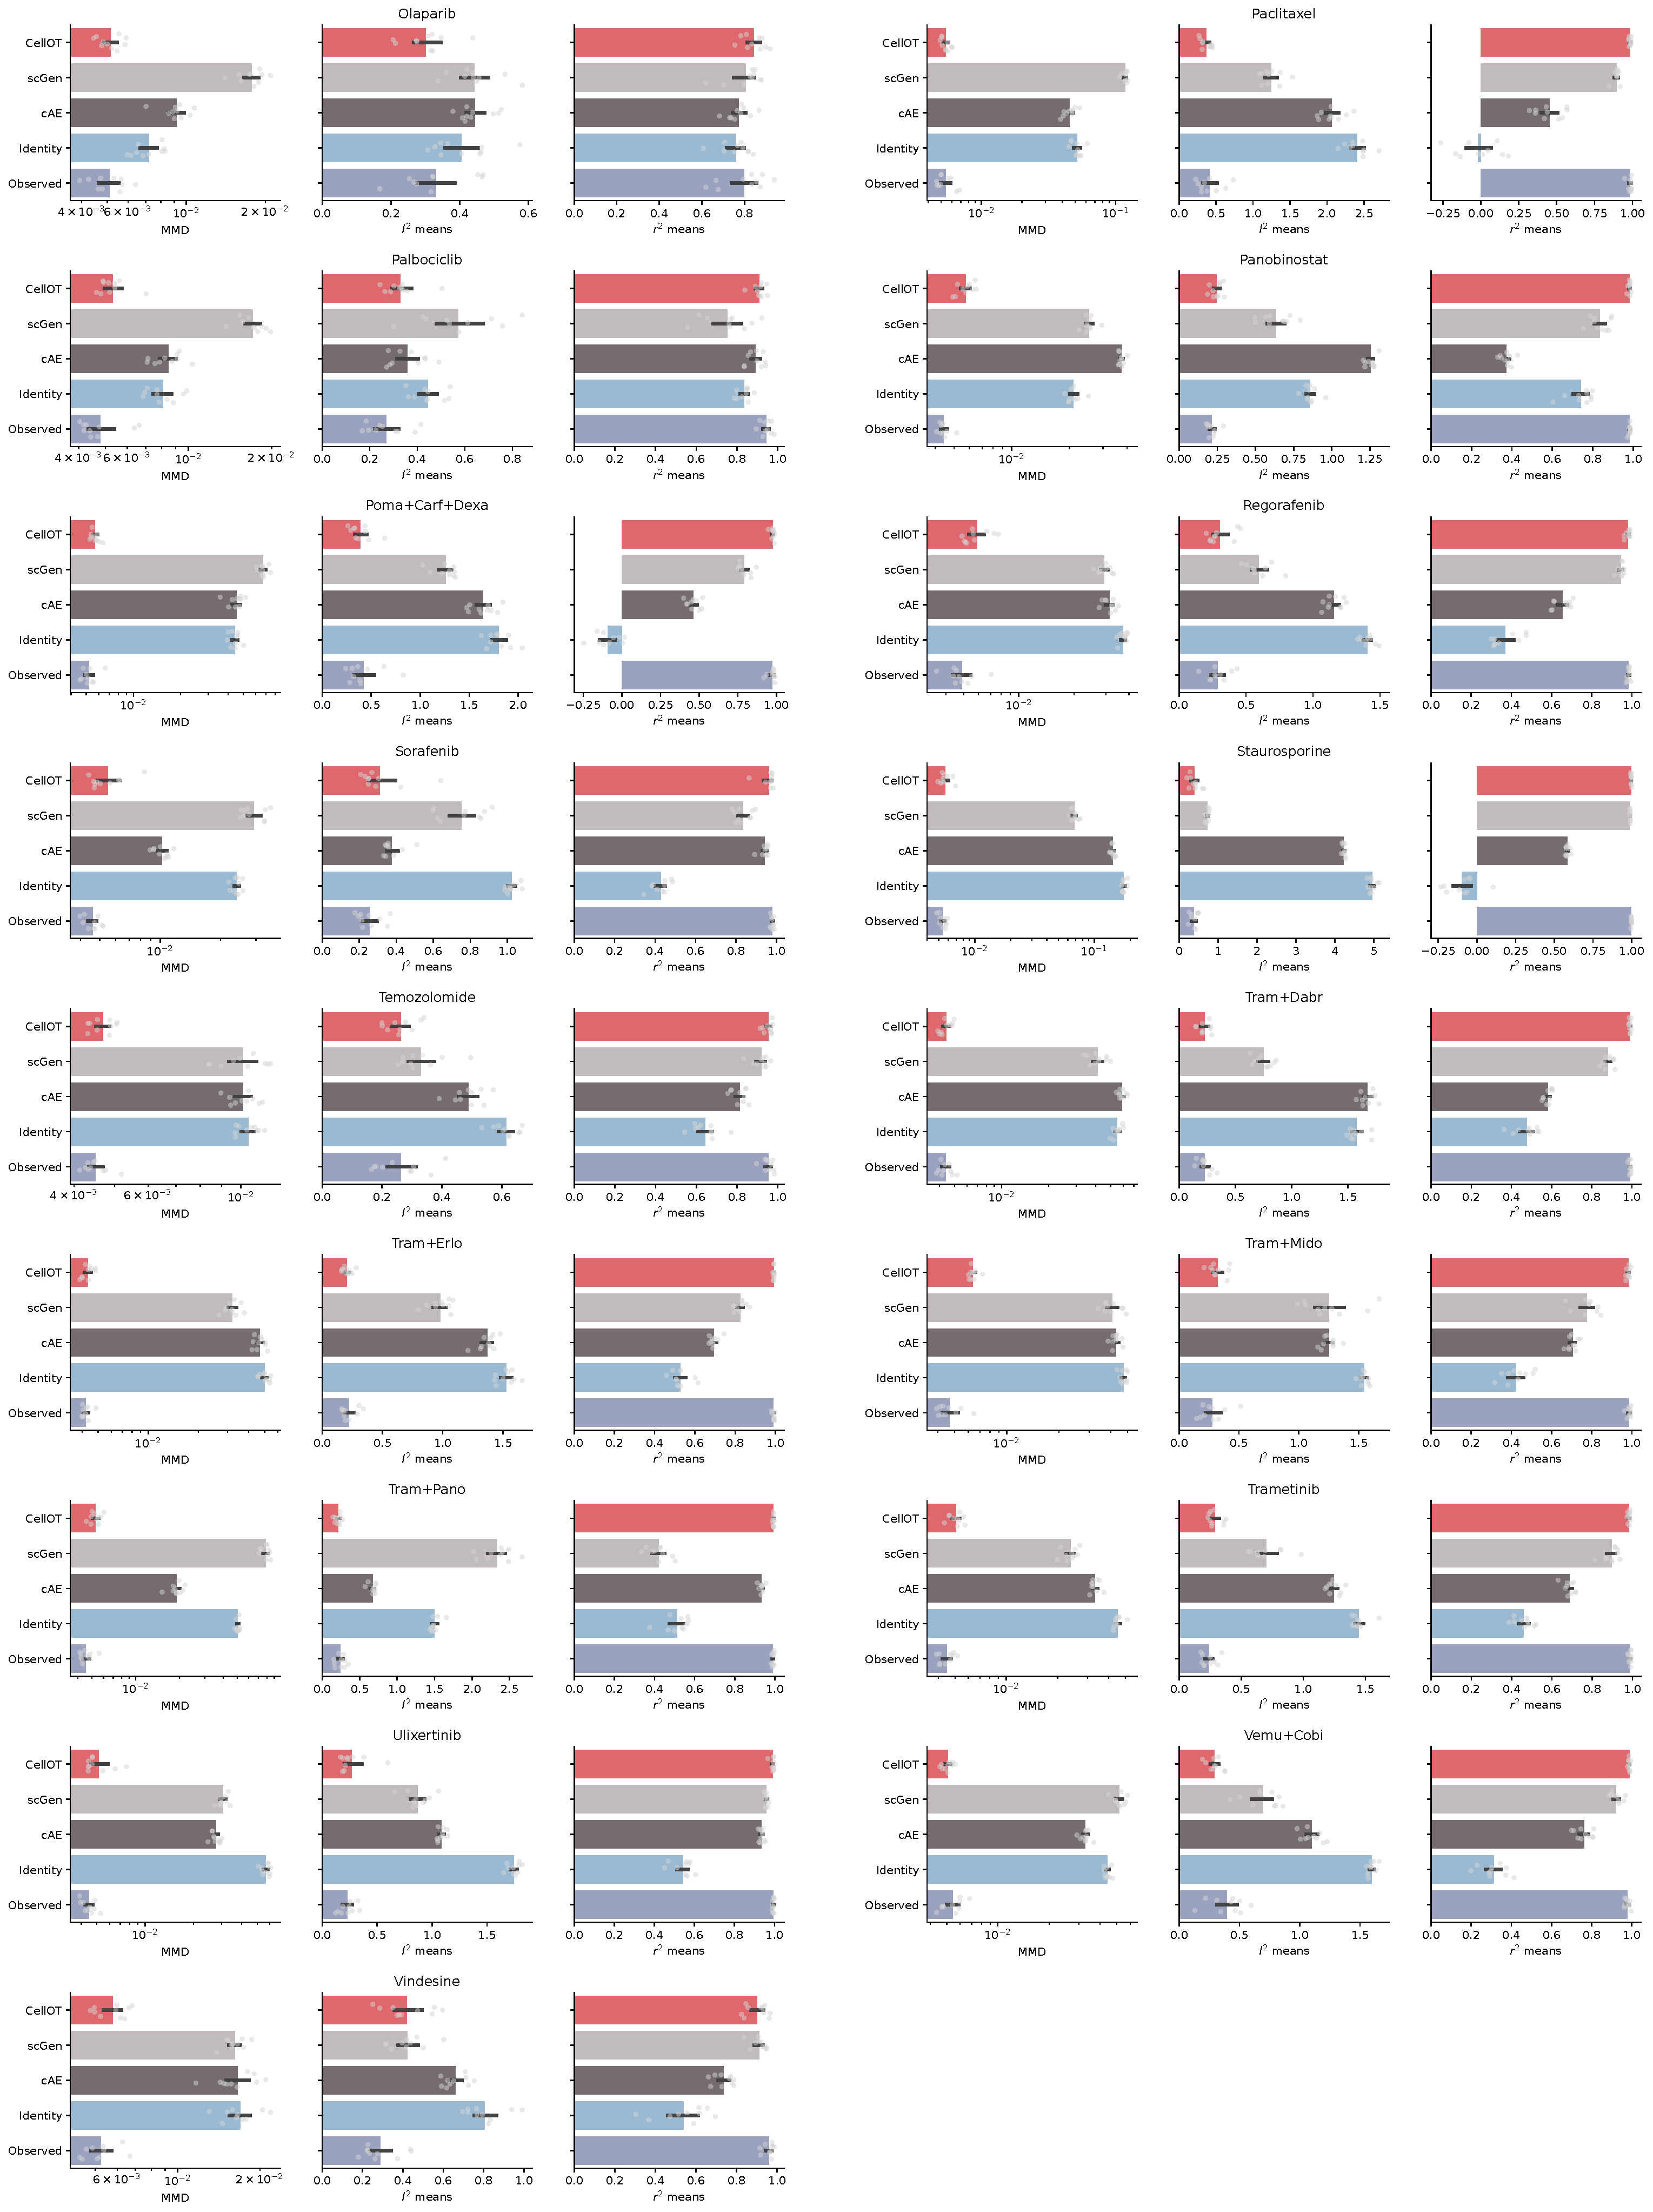
\includegraphics[width=\textwidth]{figures/cellot-methods/Bunne_Supp_Fig5_p2.pdf}
    \caption{Results on other drugs for the 4i dataset for different metrics, including MMD, $\ell_2$ feature means, and $r^2$ correlation feature means for \textsc{CellOT} as well as different baselines. Data is presented as the mean +/- standard deviation across n=10 bootstraps of the test set.}
    \label{supp_fig:4i_all_results}
\end{figure}

\begin{figure}[H]
    \centering
    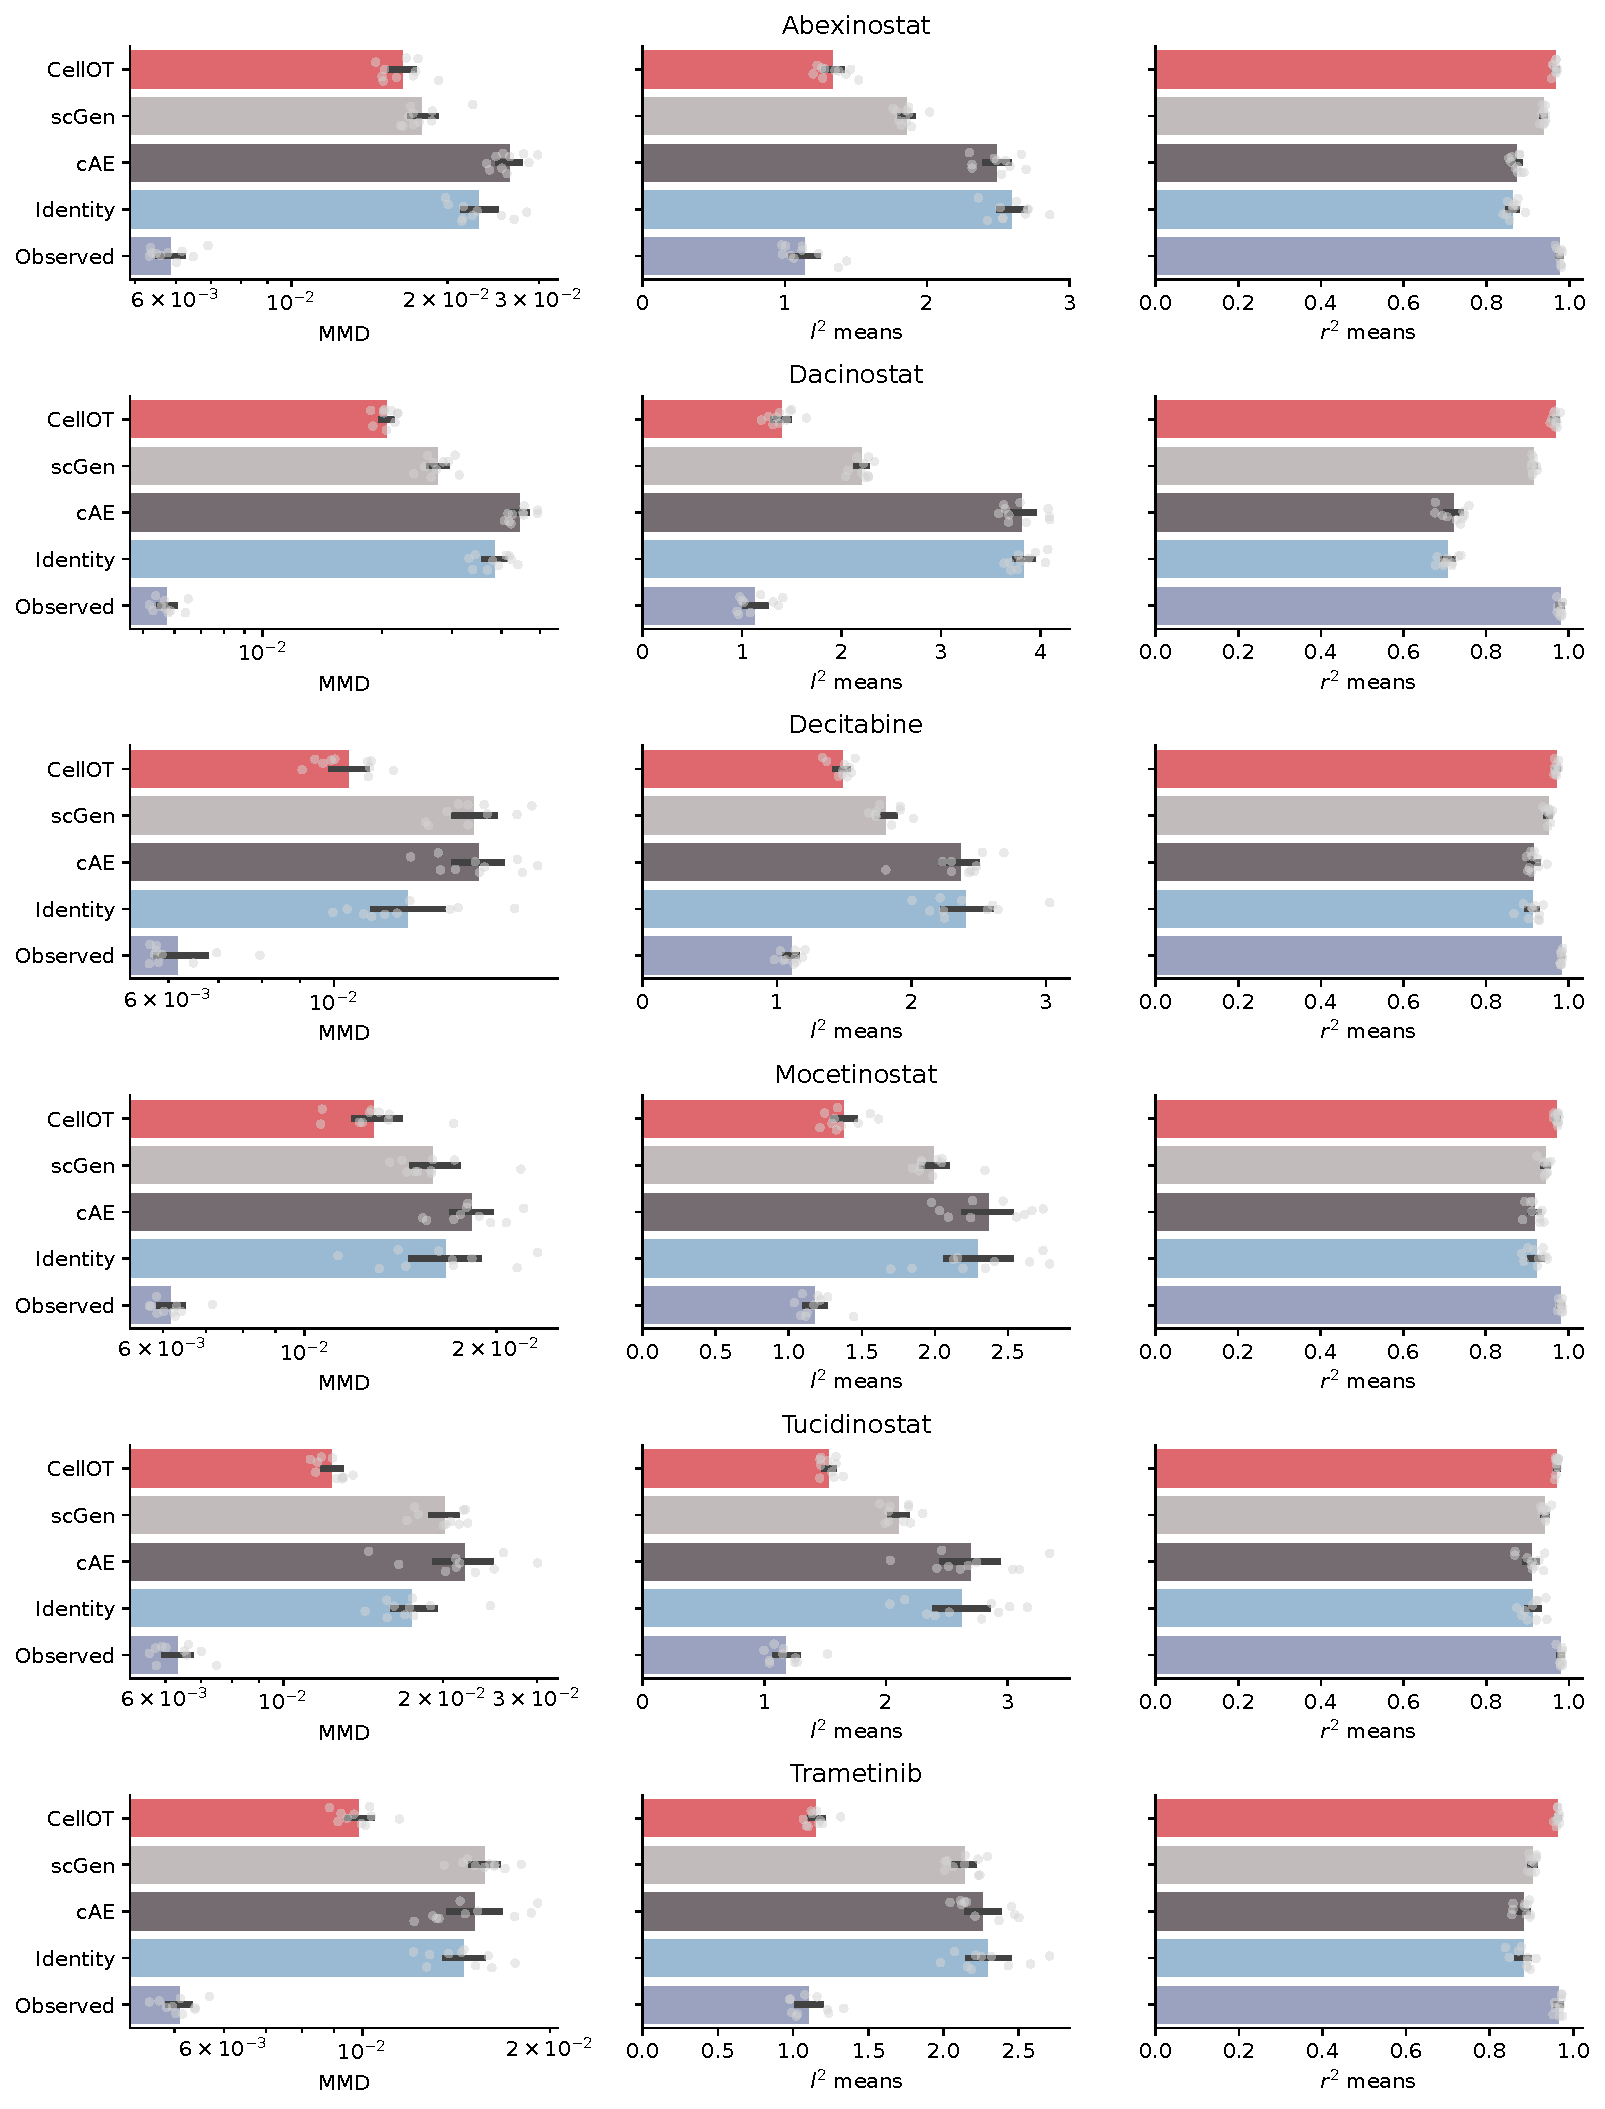
\includegraphics[width=.8\textwidth]{figures/cellot-methods/Bunne_Supp_Fig6.pdf}
    \caption{Results on other drugs for the SciPlex 3 dataset for different metrics, including MMD, $\ell_2$ feature means, and $r^2$ correlation feature means for \textsc{CellOT} as well as different baselines. Data is presented as the mean  +/- standard deviation across n=10 bootstraps of the test set.}
    \label{supp_fig:sciplex_all_results}
\end{figure}

\begin{figure}[H]
    \centering
    \includegraphics[width=\textwidth]{./figures/cellot-methods/Bunne_ED_Fig1.pdf}
    \caption{Analysis of dataset structures for the 4i dataset (\textbf{a}, \textbf{b}) and the SciPlex 3 dataset (\textbf{c}). $\textbf{a)}$ Spearman correlations between all feature pairs computed in 4i control cells (bottom) and Sorafenib-treated cells (top). Row colors show the mean value of each feature in control cells and column colors show the effect of the drug on each feature as computed by the difference in means between control and treated. Correlations that changed the most under the perturbation are highlighted in blue. $\textbf{b)}$ Density plot of feature correlations in the control setting vs. treated setting for all 35 4i treatments. Sorafenib values (corresponding to elements in $\textbf{b}$) are scattered above and light blue points correspond to blue boxes in $\textbf{b}$. $\textbf{c)}$ Feature correlation between in the control setting vs. treated setting for all cancer drugs of the SciPlex 3 dataset.}
    \label{supp_fig:data_correlation}
\end{figure}

\begin{figure}[H]
    \centering
    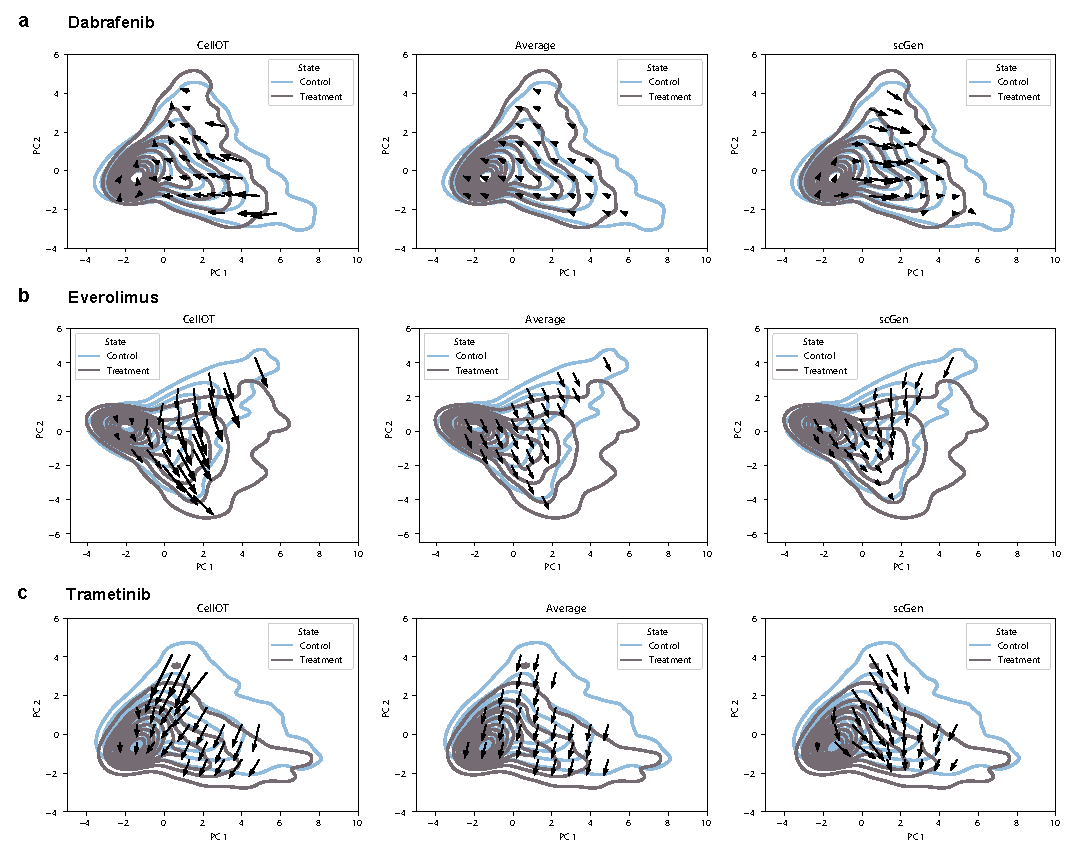
\includegraphics[width=\textwidth]{./figures/cellot-methods/Bunne_ED_Fig2.pdf}
    \caption{Visualization of the learned vector field describing the perturbation response on the single-cell level for \textbf{a)} Dabrafenib, \textbf{b)} Everolimus, and \textbf{c)} Trametinib of the 4i dataset for \textsc{CellOT}, the average effect, and \textsc{scGen} on the first two principal components. Cellular responses are computed as the predicted treated state minus the observed control state for each individual cell. Arrow tails are placed in a grid within PC space and arrow heads correspond to the average response of cells within each neighborhood, projected into PC space.}
    \label{supp_fig:4i_vector_fields}
\end{figure}

\begin{figure}[H]
    \centering
    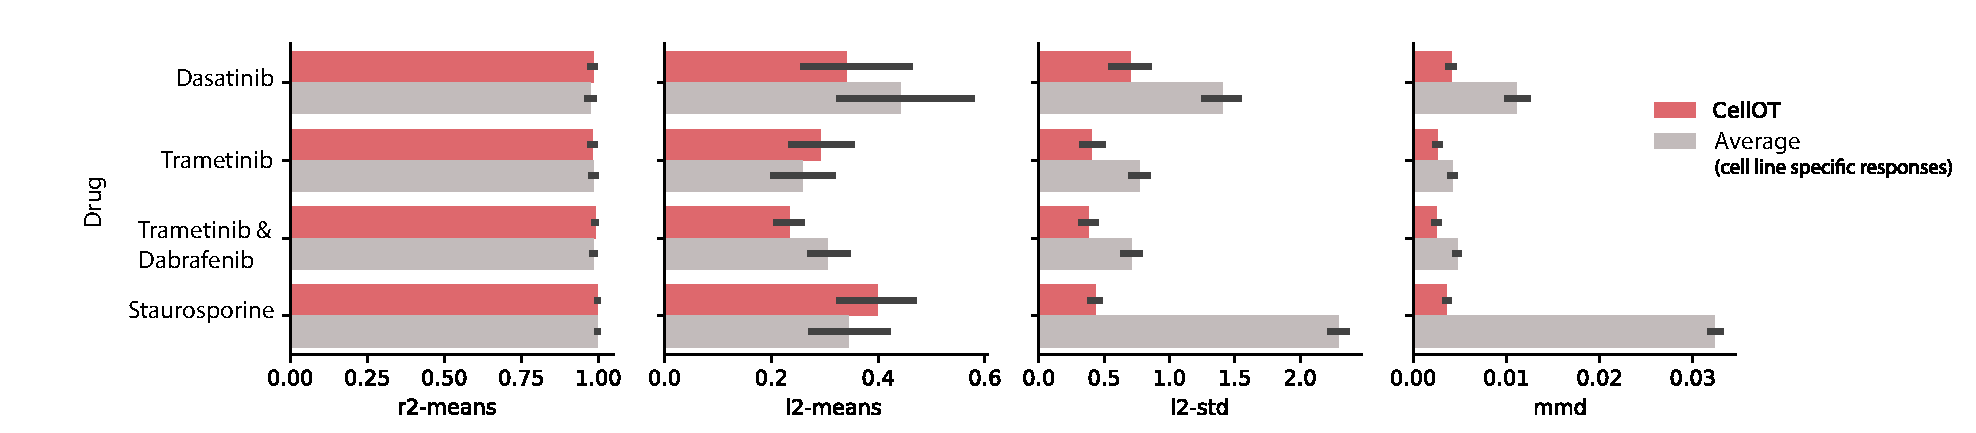
\includegraphics[width=1.05\textwidth]{figures/cellot-methods/Bunne_Supp_Fig13.pdf}
    \caption{Results of predicting perturbation effects of a selection of cancer drugs on 4i data using \textsc{CellOT} and a baseline that predict the average perturbation effect of each cell line (\textsc{Average}). Contrary to \textsc{CellOT}, the baseline requires cell typing, and annotation might not always be trivial. For example, in this setting, cell type markers are affected by the perturbation itself. The benchmark is conducted w.r.t. different metrics, including MMD, $r^2$ correlation feature means, $\ell_2$ feature means, and standard deviation. Data are presented as the mean +/- standard deviation across n=15 bootstraps of the test set.}
    \label{supp_fig:comparison_cellot_average}
\end{figure}

% TODO: shorten caption
\begin{figure}[b!]
    \centering
    \includegraphics[width=0.95\textwidth]{./figures/cellot-methods/Bunne_ED_Fig3.pdf}
    \caption{(caption next page)}
    \label{supp_fig:4i_analysis_extended}
\end{figure}
\addtocounter{figure}{-1}
\begin{figure}[t!]
\caption{\textbf{a)} High similarity of measured and CellOT-predicted single-cell pERK (phosphor ERK1/2) values at the single-cell level. Scatter plots compares the relationship between measured pERK values of cells (left) treated with Midostaurin (green dots), Palbociclib (blue dots), Panobinostat (red dots), and MLN2480 (purple dots) or (right) predicted for those drugs along the horizontal axis to their corresponding 3NN cells on the vertical axis. For details on the generation of 3NN data. X mark, square, inverted triangle, and circle represent the mean of the respective measurements per drug. The dashed gray line indicates the diagonal along which the measurements would correlate perfectly. \textbf{b )} The high similarity of measured and CellOT-predicted single-cell pERK (phosphor ERK1/2) values at the population level across all drug perturbations. Drug average of measured (blue dots) and predicted (green dots) pERK values compared to their respective 3NN measurement. Drug treatments highlighted in color correspond the those presented in panel \textbf{a}. The dashed gray line indicates the diagonal along which the measurements would correlate perfectly. \textbf{c)} Projection of measured perturbed and predicted perturbed cells in a shared UMAP space. Each cell is color-coded according to the perturbation from which it originates. \textbf{d)} Projection of mean-corrected measured perturbed cells in a UMAP space. Each cell is color-coded according to the perturbation from which it originates. Mean correction was achieved by subtracting calculating the mean of every feature for all cells in the control condition and subtracting the calculated feature means from the feature values of individual cells. \textbf{e)} Projection of single-cell corrected, predicted perturbed cells in a UMAP space. Each cell is color-coded according to the perturbation model with which it was predicted. \textbf{f)} Projection of single-cell corrected, predicted perturbed cells in a UMAP space. Each cell is color-coded according to its assignment to one of the 12 cell states. \textbf{g)} Feature value overview of the 12 identified cell states in DMSO-treated (Control) cells. Each column represents a cell state, each row a feature. Circles are colored and scaled based on feature value, from small size in blue for low feature values, to large circles in yellow for high feature values.
%\textbf{h-j)} Drug effect overview of the 12 identified cell states in \textbf{h)} Staurosporine (apoptosis ind.m apoptosis inducer, \textbf{i)} Trametinib (MEKi, MEK inhibitor), MLN2480 (panRAFi, panRAF inhibitor), \textbf{j)} Trametinib + Midostaurin (Tram + Mido, MEK inhibitor + pan Receptor Tyrosine Kinase inhibitor (panRTK)), Midostaurin (panRTK). Each column represents a cell state, rows represent features. `cell-' stands for mean cell intensity. Circles are scaled based on drug effect, the larger the $\pm$ effect the larger the circles. Negative values are encoded in hues of blue, positive values in red hues of the respective circles.
%\textbf{k)} Effect of drug treatments on levels of cleaved Caspase 3 (cleaved Caspase 3) in the 12 identified cell states. Each column represents a cell state, each row a drug treatment. Circles are scaled based on drug effect, the larger the $\pm$ effect the larger the circles.
}
\end{figure}

\begin{figure}[H]
    \centering
    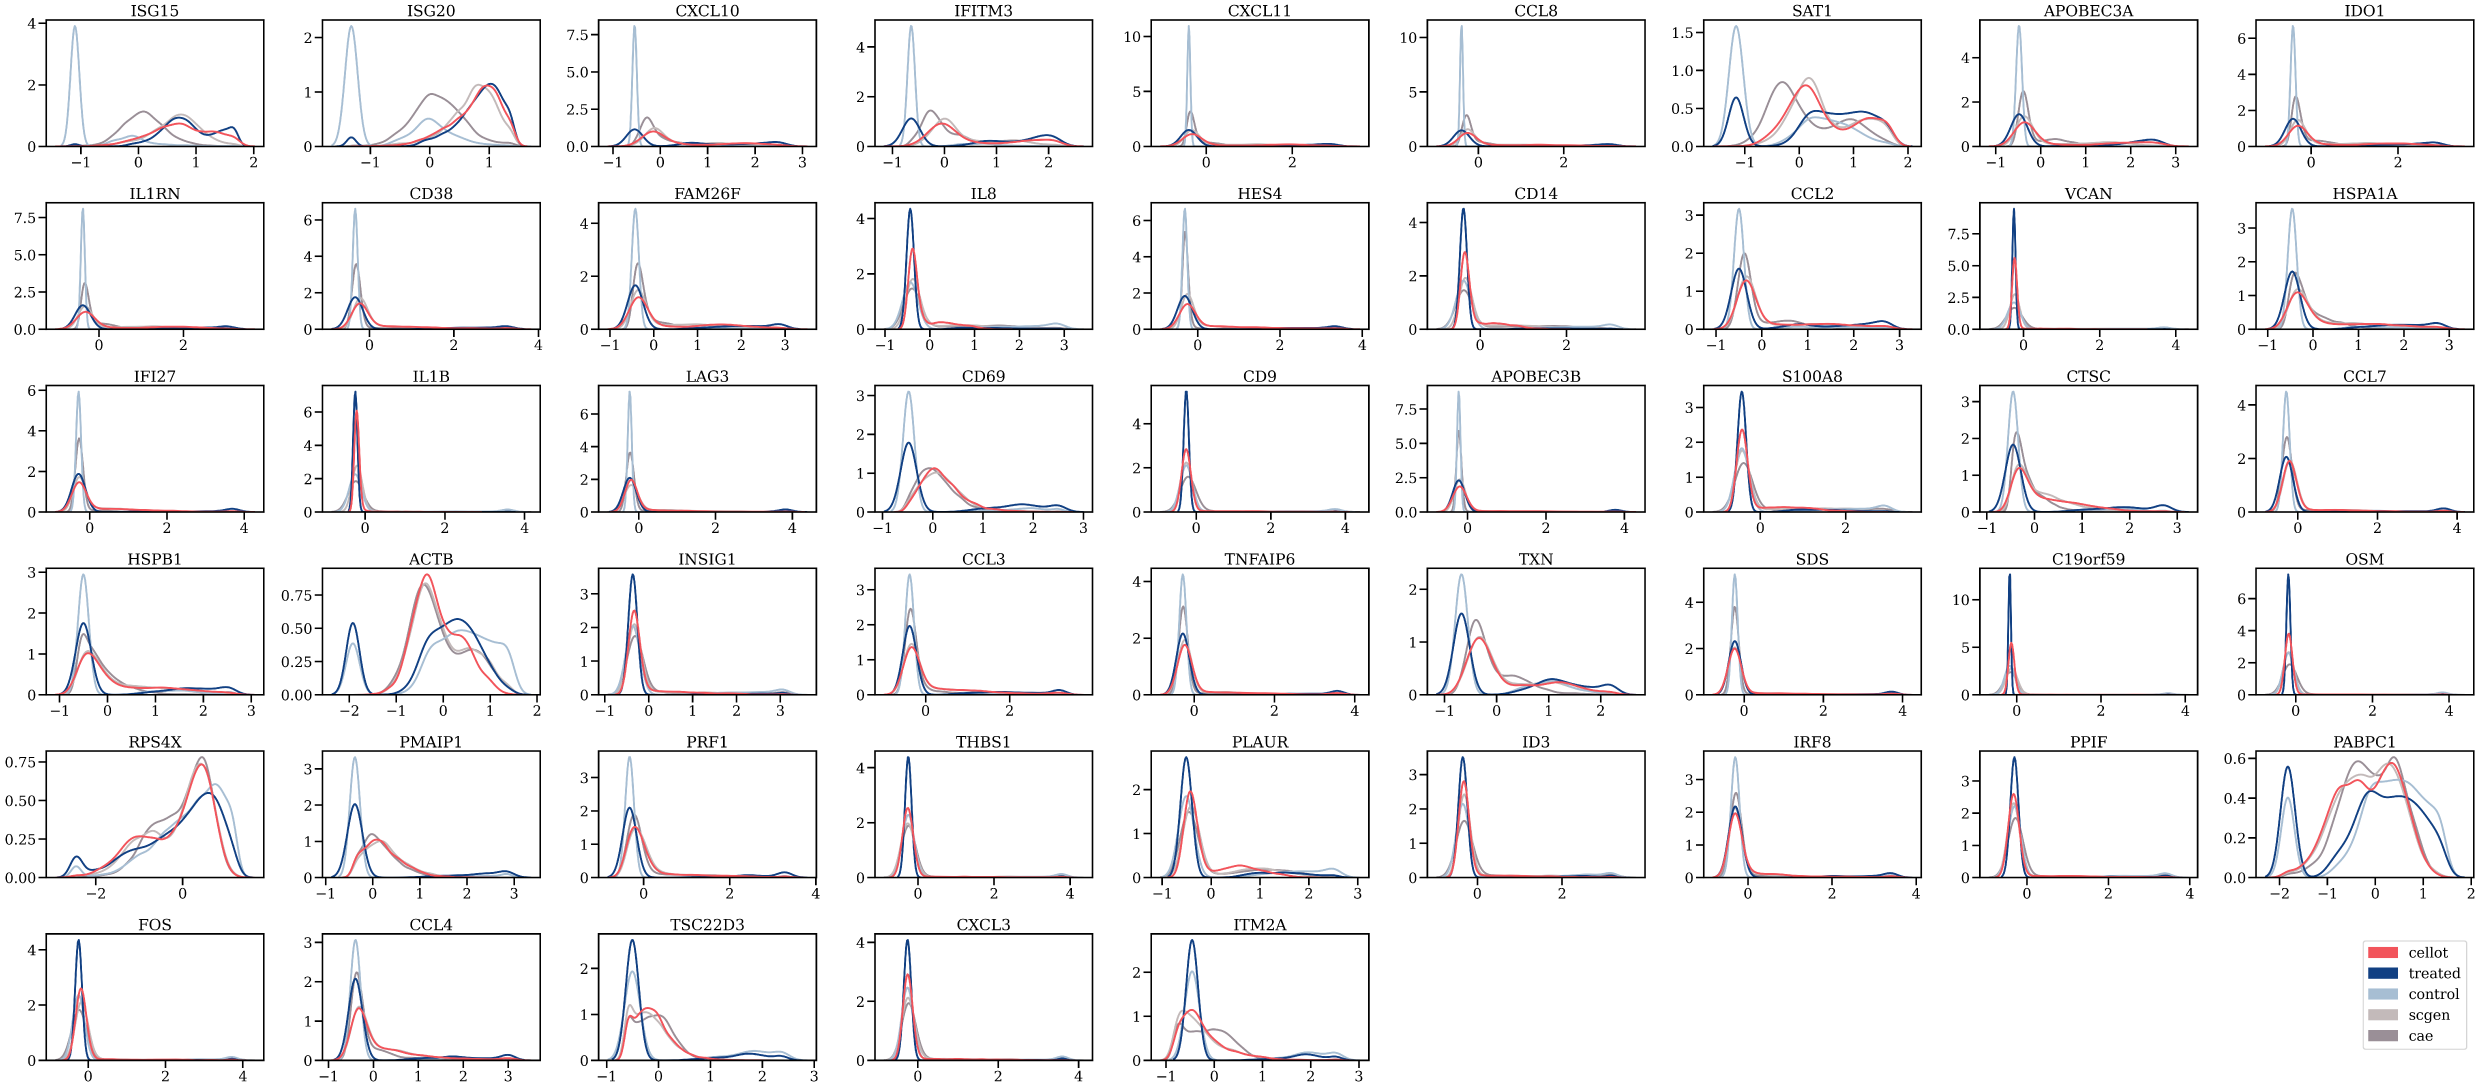
\includegraphics[width=\textwidth]{figures/cellot-methods/Bunne_Supp_Fig9.png}
    \caption{Complete set of predicted marginals for scRNA-seq profiled cells of holdout cells pooled across all lupus patients.}
    \label{supp_fig:lupus_all_marginals_iid}
\end{figure}


\begin{figure}[H]
    \centering
    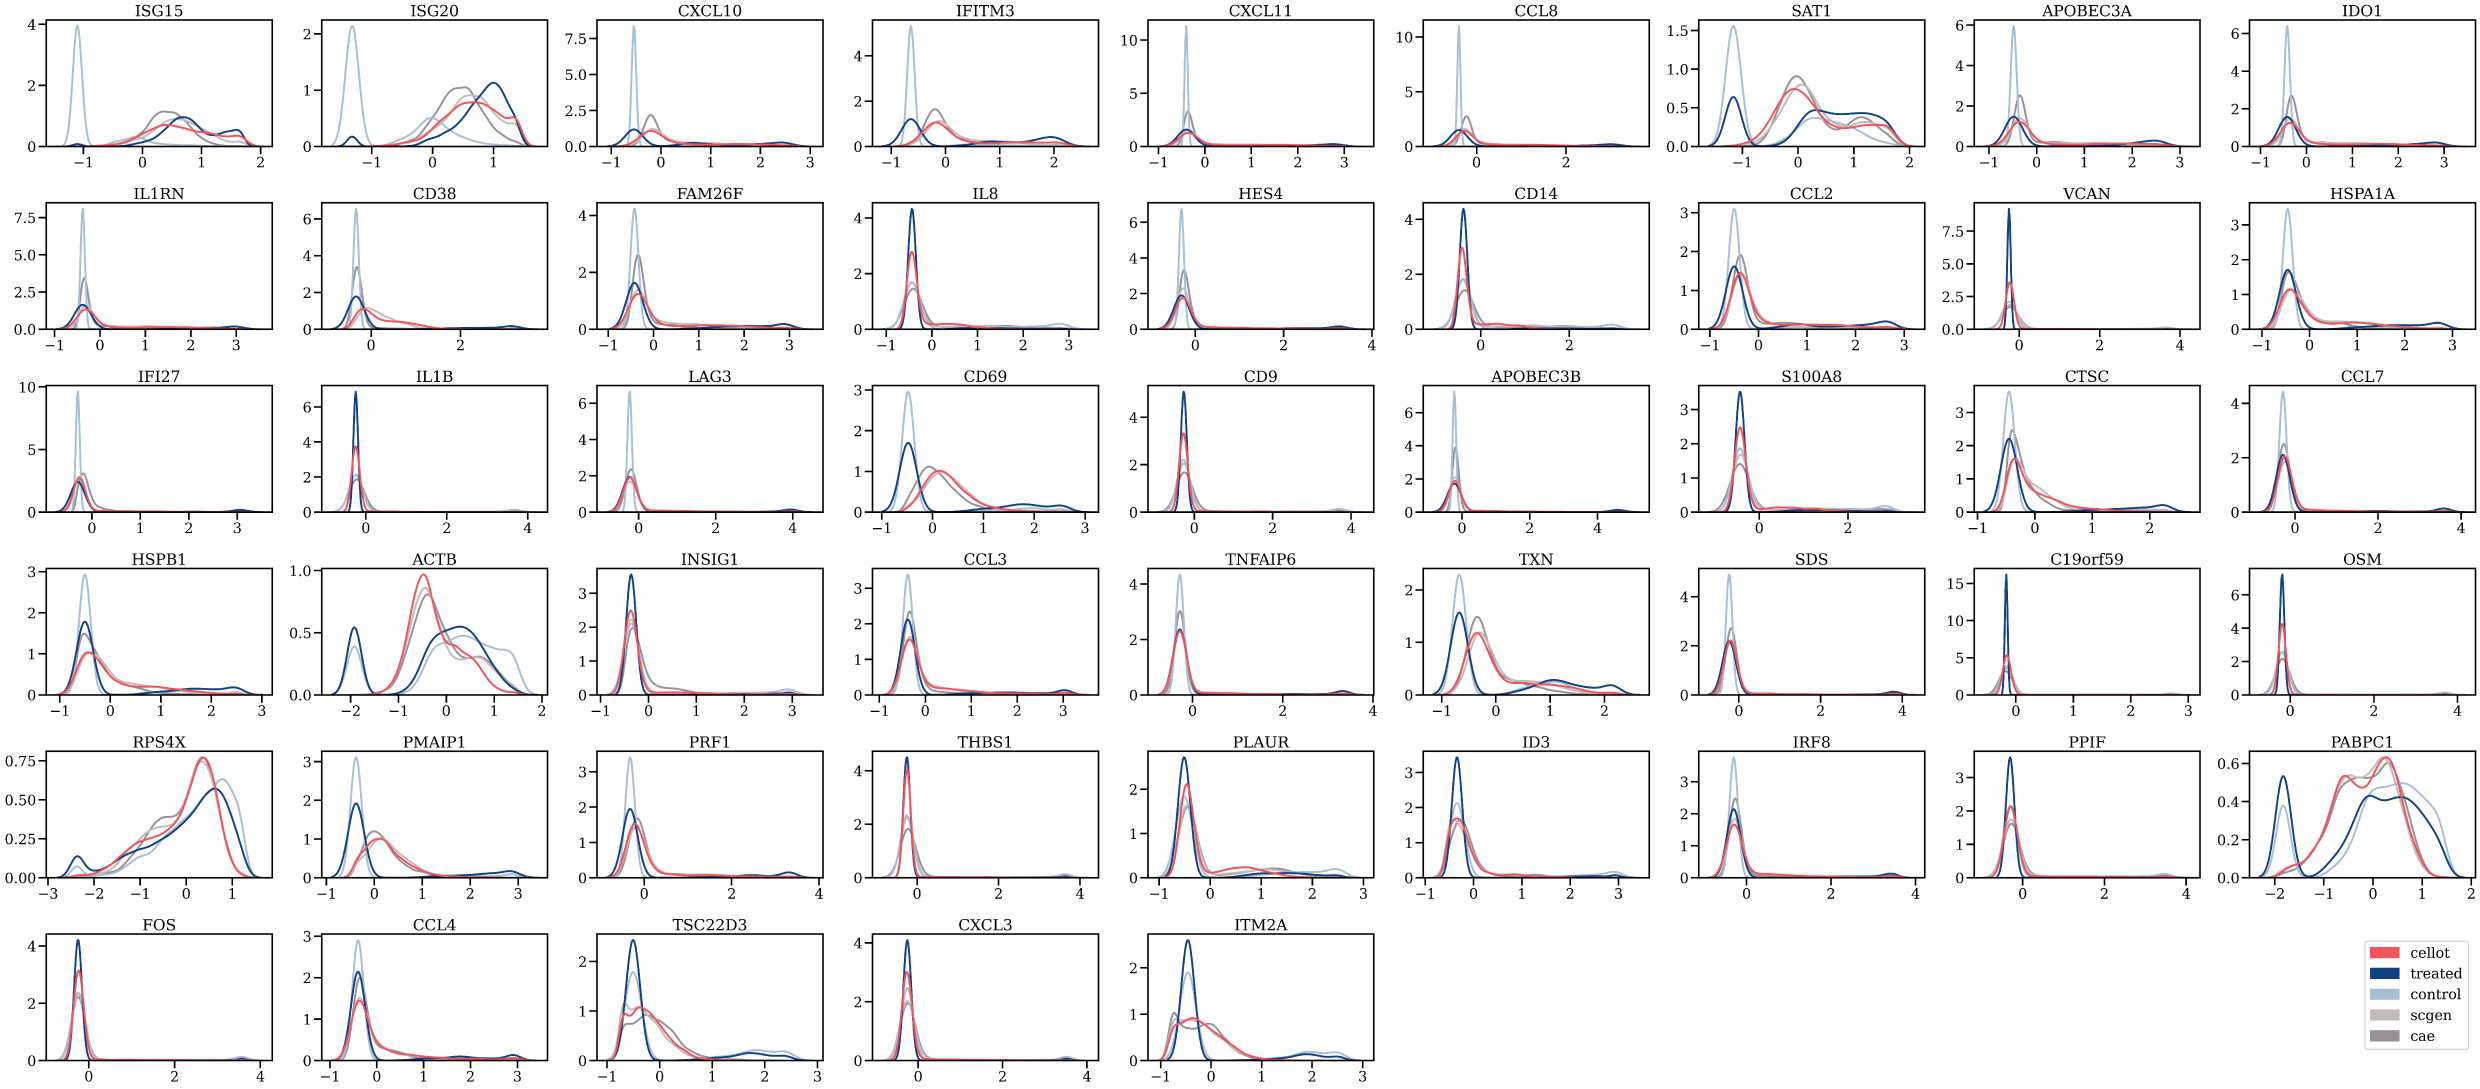
\includegraphics[width=\textwidth]{figures/cellot-methods/Bunne_Supp_Fig10.png} 
    \caption{Complete set of predicted marginals of scRNA-seq profiled cells from a single holdout lupus patient (id=1015), treated with an IFN-$\beta$ perturbation.}
    \label{supp_fig:lupus_all_marginals_ood}
\end{figure}


\begin{figure}[H]
    \centering
    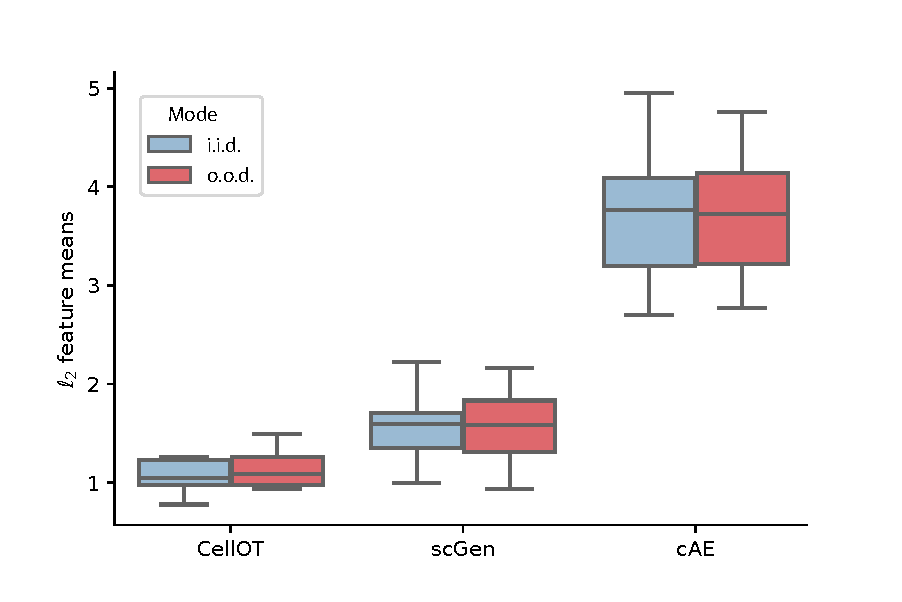
\includegraphics[width=.65\textwidth]{figures/cellot-methods/Bunne_Supp_Fig8.pdf}
    \caption{$\ell_2$ feature means between the predicted distribution and the observed treated distribution for the lupus patients dataset across all holdout samples in the i.i.d.~and o.o.s.~settings. Boxplots show the median and quartiles of the distribution for 10x bootstraps for each of the n=8 samples.}
    \label{supp_fig:lupus_iid_ood_l2ds}
\end{figure}


\begin{figure}[H]
    \centering
    \includegraphics[width=\textwidth]{figures/cellot-methods/Bunne_Supp_Fig11.png}
    \caption{UMAP projections of \textsc{CellOT}, different baselines, and na\"ive OT maps for predicting patient responses to IFN-$\beta$ treatment for different lupus patients taken as holdout (in the o.o.d. setting). For each method and setting, we display the measured perturbed and predicted perturbed cells.}
    \label{supp_fig:lupus_umaps_all}
\end{figure}

\begin{figure}[H]
    \centering
    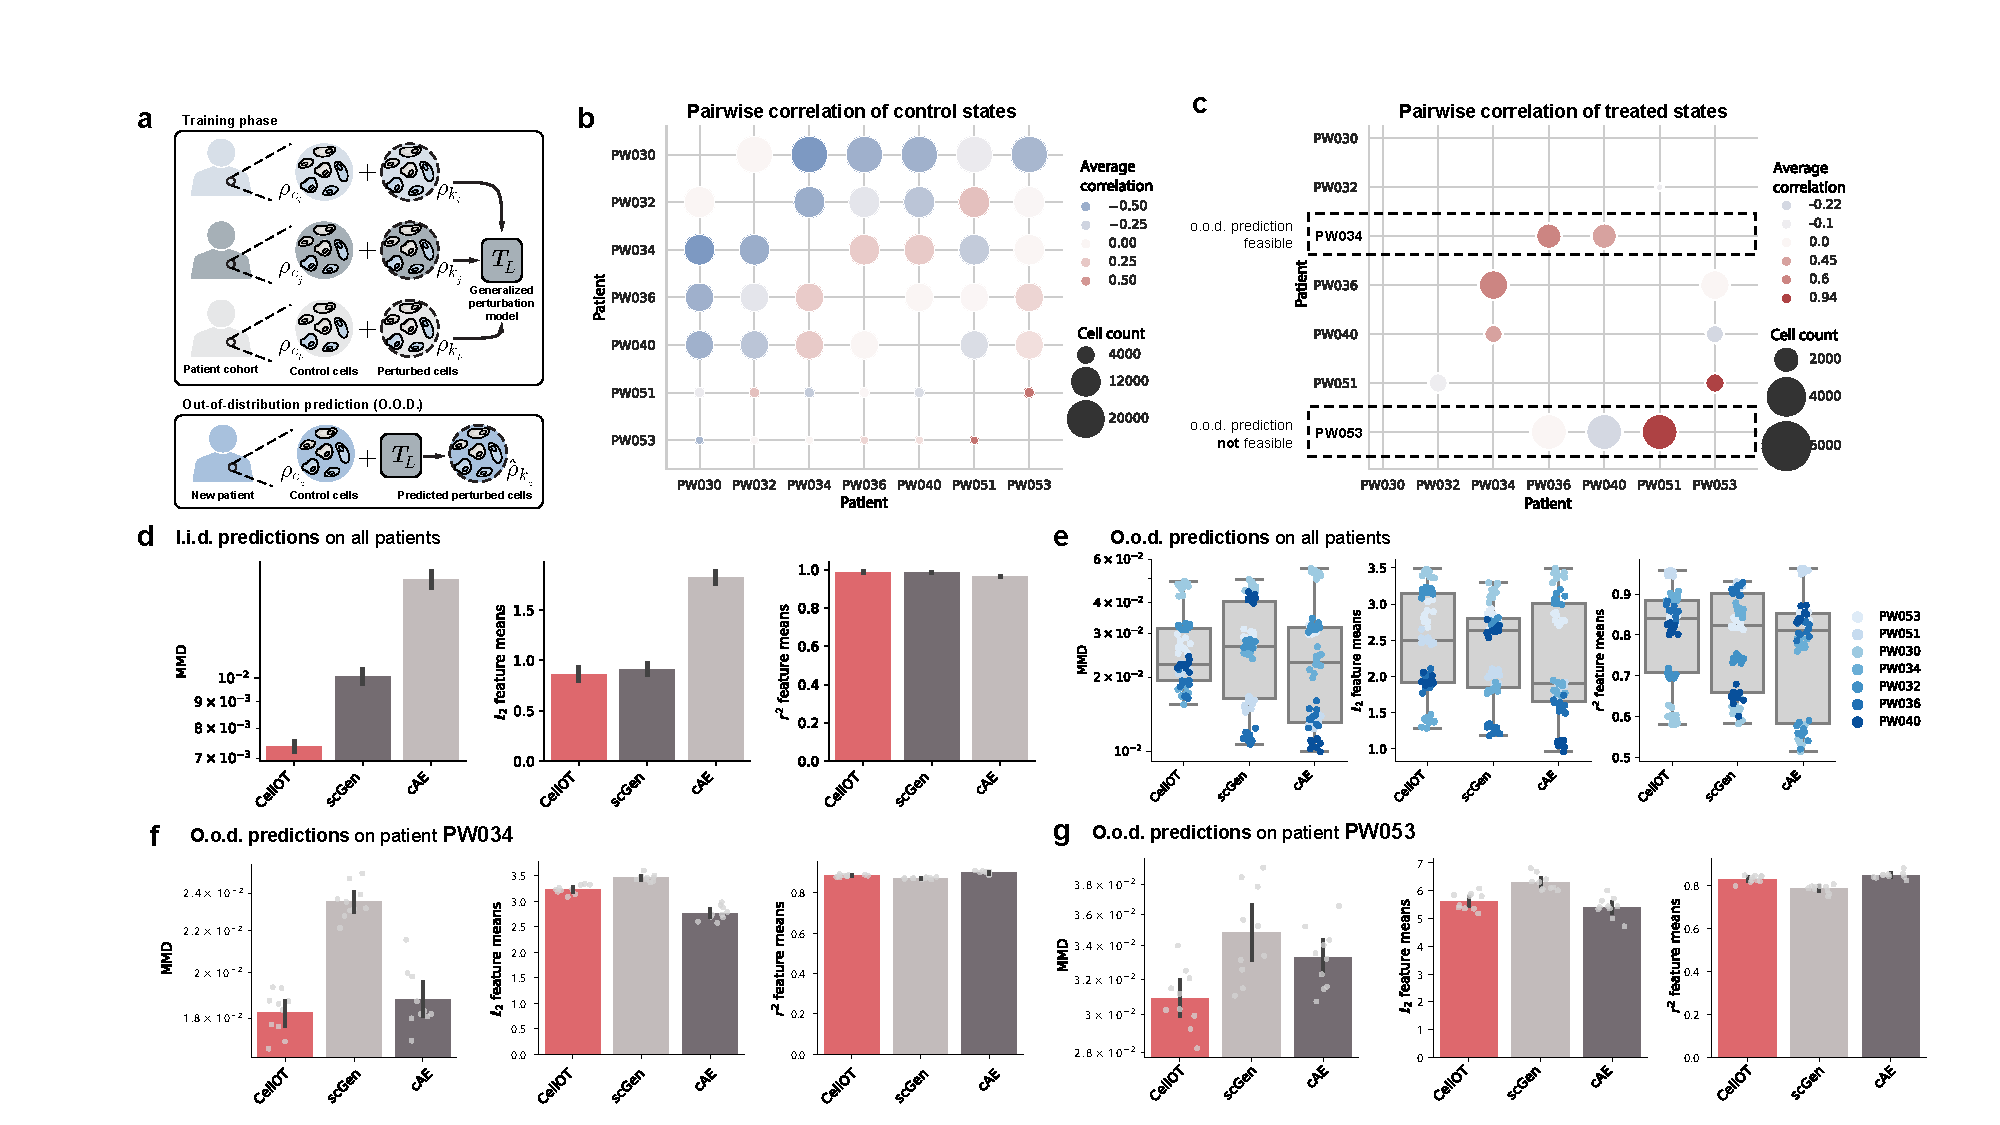
\includegraphics[width=1.05\textwidth]{./figures/cellot-methods/Bunne_ED_Fig6.pdf}
    \caption{Analysis and results of the glioblastoma dataset consisting of seven patients. \textbf{a)} Cells from seven glioblastoma patients are measured in an untreated and Panobinostat-treated state. For each sample, we train two models, an o.o.d.~model trained on cells from all other samples but the holdout patient we test on and an i.i.d.~model trained with additional access to half of the cells in the holdout sample.
    \textbf{b)} Pairwise average correlation of the PCA embeddings of the control states between patients. \textbf{c)} Pairwise average correlation of the PCA embeddings of the treated states between patients, masked to only those patient pairs that showed a positive correlation in the control states. Only patient PW034 positively correlates with all other patients. Other patients, such as PW053, correlate and anti-correlate with other patients in the treated state.
    Performance comparison between \textsc{CellOT} and baselines for different metrics in the \textbf{d)} i.i.d. setting (mean standard deviation across 7 samples, 10 bootstraps of the test set per sample),
    \textbf{e)} o.o.d. setting for all patients (box plots show median, minima, and maxima)
    \textbf{f)} o.o.d. setting for a patient positively correlating with all patients that are also similar in the control state,
    \textbf{g)} o.o.d. setting for a patient where similar patients in the control state show different responses (correlation and anti-correlation) in the treated states. Data in \textbf{f} and \textbf{g} are presented as the mean +/- standard deviation across n=10 bootstraps of the test set.
    }
    \label{supp_fig:gbm_patients_iid_ood}
\end{figure}

\begin{figure}[H]
    \centering
    \includegraphics[width=\textwidth]{./figures/cellot-methods/Bunne_ED_Fig4.pdf}
    \caption{Analysis and further results of the cross species dataset. \textbf{a)} Pairwise average correlation of the PCA embeddings of the control states between species. \textbf{b)} Pairwise average correlation of the PCA embeddings of the treated states between patients, masked to only those patient pairs that showed a positive correlation in the control states. Only rat and mouse show consistent responses, i.e., a positive correlation of the control states and non-negative correlation of the respective target cells, and are thus chosen for the o.o.d. analysis. I.i.d. and o.o.d. results measured in the average gene expression for both \textbf{d)} \textsc{CellOT} and \textbf{c)} \textsc{scGen}.}
    \label{supp_fig:crossspecies_ood_analysis}
\end{figure}


\begin{figure}[H]
    \centering
    \includegraphics[width=\textwidth]{./figures/cellot-methods/Bunne_ED_Fig5.pdf}
    \caption{
    Integration of predicted and observed perturbed state in the statefate dataset. Joint UMAP projections are computed for observed, \textsc{CellOT}, and \textsc{scGen} predictions. In each axis, projections 
 are colored by cell type (left), \textsc{CellOT} predictions (middle), and \textsc{scGen} predictions (right). For both our method \textsc{CellOT} and the baseline \textsc{scGen}, the UMAP highlights the observed and predicted perturbed cell states.
    }
    \label{supp_fig:statefate_shared_umaps}
\end{figure}


\begin{figure}[H]
    \centering
    \includegraphics[width=.5\textwidth]{figures/cellot-methods/Bunne_Supp_Fig12.png}
    \caption{Performance w.r.t. the MMD metric between measured perturbed and predicted perturbed cells by \textsc{CellOT}, different baselines, and nai\"ve OT maps on predicting cell differentiation of the statefate data over 4 and 6 days, respectively.
    }\label{supp_fig:statefate_days_all_methods}
\end{figure}


%%%%%%%%%%%%%%%%%%%%
%%%%%%%%%%%%%%%%%%%%
%%%%%%%%%%%%%%%%%%%%
%%%%%%%%%%%%%%%%%%%%
%%%%%%%%%%%%%%%%%%%% CURR SPOT
%%%%%%%%%%%%%%%%%%%%
%%%%%%%%%%%%%%%%%%%%
%%%%%%%%%%%%%%%%%%%%
%%%%%%%%%%%%%%%%%%%%


%\begin{figure}[H]
%    \centering    \includegraphics[width=\textwidth]{figures/cellot-methods/Bunne_Supp_Fig3.png}
%    \caption{Predicted and observed marginals for all features of cells profiled by scRNA-seq of the SciPlex 3 dataset treated with Givinostat. The top 50 marker genes for the perturbation are shown.}
%    \label{supp_fig:sciplex_all_marginals_gavinostat}
%\end{figure}
%
%\begin{figure}[H]
%    \centering
%    \includegraphics[width=\textwidth]{figures/cellot-methods/Bunne_Supp_Fig4.png}
%    \caption{Predicted and observed marginals of cells profiled by scRNA-seq of the SciPlex 3 dataset treated with Trametinib. The top 50 marker genes for the perturbation are shown.}
%    \label{supp_fig:sciplex_all_marginals_trametinib}
%\end{figure}
%
%
%\begin{table}[h]
%    \caption{Hyperparameter search for scRNA autoencoders.}
%    \centering
%    \begin{tabular}{lcc}
%         \textbf{Parameter} & \textbf{Values} & \textbf{Selected} \\
%         \midrule
%         latent dimension & 50, 100 & 100 \\
%         num layers & 2, 3 & 2 \\
%         layer width & 256, 512 & 512 \\
%         dropout rate & 0, 0.05, 0.1, 0.2 & 0 \\
%         weight decay & 0, 1e-5, 1e-3 & 1e-5 \\
%         scheduler.step\_size & 10k, 50k, 100k & 100k \\
%         scheduler.gamma & 0.1, 0.25, 0.5, 0.9 & 0.5 \\
%    \end{tabular}
%    \label{tab:hyperparams}
%\end{table}

\cleardoublepageempty{}

\section{Exploring the clinical utility of single-cell perturbation responses}
\begin{figure}[h]
  \begin{center}
    \includegraphics[width=0.95\textwidth]{figures/cellot-cohort/supplement/normalization.pdf}
  \end{center}
  \caption{
  Cohort normalization by removal of background intensity.
  a) distribution of intensity values of two features (pERK, top and pAKT, bottom) in the control state and secondary control (background). The secondary control measures the intensity generated when the probe is missing, considered to be uninformative "background" noise.
  b) Distribution of control intensities after removal of background intensity.
  c) For each patient the average state for all treatments are taken. Then within each condition, patient-patient similarities are computed as the euclidean distance between their averages. Replicates are much closer than unrelated samples, suggesting that the normalization has worked.
  }
\label{fig:cellot-cohort-normalization}
\end{figure}

\begin{figure}[h]
  \begin{center}
    \includegraphics[width=0.95\textwidth]{figures/cellot-cohort/supplement/iid-metrics-drugs.pdf}
  \end{center}
  \caption{\textsc{CellOT} consistently improves metrics computed to compare (iid) predicted cell states with observed treated cell states.
  Three metrics are considered (MMD, euclidean distance between feature means and the EMD of pERK). 
  Colored squares indicate that there is a significant difference (t-test, $p < 0.01$ between \textsc{CellOT} and the baseline over the whole cohort.
  Blue hues indicate that \textsc{CellOT} improves over the baseline.
  }\label{fig:cellot-cohort-iid-metrics}
\end{figure}

\begin{figure}[h]
  \begin{center}
    \includegraphics[width=0.95\textwidth]{figures/cellot-cohort/supplement/knn-enrichment-iid.pdf}
  \end{center}
  \caption{
  kNN enrichment scores (k=50) of predicted cells given an even mixtures of predicted and treated cells. For each sample, nearest neighbors are computed over an even split of treated and (i.i.d.) predicted cells for each treatment. Barplots are drawn over the distribution of average enrichment score for each treatment. Scores $< 0.5$ indicate that predicted states are grouped more with each other in isolation and thus do not faithfully represent the observed treated states.
  }
\label{fig:cellot-cohort-iid-knn}
\end{figure}

\begin{figure}[h]
  \begin{center}
    \includegraphics[width=0.95\textwidth]{figures/cellot-cohort/ood-eval-logmmd.pdf}
  \end{center}
  \caption{
    Pairwise logMMD differences comparing \textsc{CellOT} and baseline approaches.
    For each (drug, patient) pair, models are trained on the entire cohort with that patient held out.
    Each model predicts the drug response of the heldout patient
    and logMMD values are computed between the distribution of predicted treated states and the true treated states.
    Negative values correspond to settings where \textsc{CellOT} improves over the corresponding baseline.
  }
\label{fig:ood-eval-logmmd}
\end{figure}

\begin{figure}[h]
  \begin{center}
    \includegraphics[width=0.95\textwidth]{figures/cellot-cohort/ood-eval-marker.pdf}
  \end{center}
  \caption{
    Pairwise marker EMD differences comparing $\textsc{CellOT}$ and baseline approaches.
    For each (drug, patient) pair, models are trained on the entire cohort with that patient held out.
    Each model predicts the drug response of the heldout patient
    and marker EMD values are computed between the distribution of predicted treated states and the true treated states.
    Negative values correspond to settings where $\textsc{CellOT}$ improves over the corresponding baseline.
  }
  \label{fig:ood-eval-marker}
\end{figure}

\begin{figure}
  \begin{center}
    \includegraphics[width=0.95\textwidth]{figures/cellot-cohort/ood-predict-marginals.pdf}
  \end{center}
  \caption{
    Predicted response to trametinib dabrafenib combination treatment of each heldout samples.
    Marginals are shown for the treatment's marker feature, pERK.
    The inlay shows the selected heldout sample's logMMD score against the rest of the cohort.
  }\label{fig:ood-predict-marginals}
\end{figure}

\begin{figure}
  \begin{center}
    \includegraphics[width=0.95\textwidth]{figures/cellot-cohort/progression-exclude-mykokig.pdf}
  \end{center}
  \caption{
    Sample mykokig exhibits evidence for low quality cell segmentation and is removed from the progression prediction task.
  a) Scatter plot of number of treated cells by the variance of intensity features.  Each dot corresponds to a (treatment, sample) pair and treatments of mykokig are shown in blue. Mykokig behaves as an outlier as it has much more cells per treatment than other samples and these cells have low variance in their intensity features.
  b) Morphology features of mykokig cells indicate the presence of artifacts. The cluster map shows the distribution of each extracted morphology feature (rows) for cells sampled from mykokig and a subset of 5 samples from the full cohort. A large fraction of mykokig cells exhibit a strange unique morphology pattern of small round cells.
  }\label{fig:progression-exclude-mykokig}
\end{figure}

\begin{figure}
  \begin{center}
    \includegraphics[width=0.95\textwidth]{figures/cellot-cohort/progression-exclude-motamuh.pdf}
  \end{center}
  \caption{
    The predicted responses for sample motamuh are consistently poor and the sample is therefore removed from the progression prediction task.
    Boxplots show the ranked MMD metric computed between each model's prediction and observed treated states for drugs considered in the progression prediction task.
    Results for the average model are shown in the IID and OOD setting as well as CellOT predictions in the OOD setting.
    Sample motamuh consistently ranks worst across all samples in the cohort for these prediction tasks.
  }\label{fig:progression-exclude-motamuh}
\end{figure}

\begin{figure}[h]
  \begin{center}
    \includegraphics[width=0.95\textwidth]{figures/cellot-cohort/supplement/survival-accuracies-baselines.pdf}
  \end{center}
  \caption{Progression prediction, ablation of model against number of underlying clusters and prediction model used. Baseline models do not improve over \textsc{CellOT}, which is also much less sensitive to the choice of hyperparameter, indicating that \textsc{CellOT} scDRs have a high information content.
  }
\label{fig:survival-accuracies}
\end{figure}

\cleardoublepageempty{}
\chapter{Appendix}

\section{Learning to align single-cell multi-modal profiles}
\begin{table}[ht]
\centering
\begin{tabular}{lrrrrr}
\toprule
Target B &     A &     B &      C &     D &     E \\
Source &       &       &        &       &       \\
\midrule
A      &  8,833 &   430 &    709 &     1 &     0 \\
B      &   249 &  6,710 &    536 &   526 &   681 \\
C      &   925 &   552 &  19,275 &     5 &     0 \\
D      &     0 &   326 &      2 &  7,906 &   314 \\
E      &     0 &   382 &      0 &   742 &  7,523 \\
\bottomrule
\end{tabular}
\caption{Confusion table showing branch labels of the optimal matches of cells in the simulated PROSST data, between Source and Target B. Entries on the diagonal correspond to correct matches whereas off-diagonal elements to mismatches. The overall accuracy, with respect to the branch label, equals 89\%.}
\label{tbl:prosstt_conf_SB}
\end{table}

\begin{table}
\centering
\begin{tabular}{lrrrrr}
\toprule
Target B &     A &     B &      C &     D &     E \\
Target A &       &       &        &       &       \\
\midrule
A      &  7,718 &   738 &    844 &    21 &    19 \\
B      &   518 &  6,312 &    785 &   679 &  1190 \\
C      &   777 &   865 &  18,460 &    20 &    42 \\
D      &    83 &   469 &     36 &  8,054 &   248 \\
E      &    25 &   904 &     66 &   517 &  7,232 \\
\bottomrule
\end{tabular}
\caption{Confusion table showing branch labels of the optimal matches of cells in the simulated PROSST data, between Target A and Target B. Entries on the diagonal correspond to correct matches whereas off-diagonal elements to mismatches. The overall accuracy, with respect to the branch label, equals 84\%.}
\label{tbl:prosstt_conf_AB}
\end{table}

\begin{figure}[htb]
    \centering
    \includegraphics[width=1\textwidth]{figures/integration/3tech-pseudotime-kde.png}
    \caption{
    Evaluation of cross-technology cell matches made by SCIM on the simulated data with three technologies. 
    The pairwise matching is attained for Source-Target A, Source-Target B, and Target A-Target B, respectively. The sink edge capacities were unbounded in all cases.
    Here, we show a density plot for matched pseudotime values between the source technology and the target technology,
    colored by the branch label. Mismatched cells are colored in grey.
    The tree defining the temporal branching process can be found in Figure \ref{fig:prosstt5-pseudotime-inverted}, left.
    Marginal distributions of cell pseudotime for each branch is shown on the top and right.
    }
    \label{fig:prosstt5-3tech-pseudotime}
\end{figure}

\begin{table}
\centering
\begin{tabular}{l|llllll}
\toprule
  method & accuracy & \#null matches & Spearman & Pearson \\
\midrule
 SCIM    &   86\% &  1,590  & 0.83  & 0.86\\
 MATCHER &   4\%  & 25,510  & -0.21 & -0.19\\
\bottomrule
\end{tabular}
\caption{The matching results on the PROSSTT dataset, where the SCIM matching algorithm was applied to SCIM shared latent codes and the MATCHER latent representation. The table depicts accuracy with respect to branch label, null node matches and the correlation coefficients for the pseudotime between matched source and target cells.}
\label{tbl:prosstt_matcher}
\end{table}

\begin{figure}[htp]
    \centering
    \includegraphics[width=1.0\textwidth]{figures/integration/matcher-pseudotime-kde.png}
    \caption{
    Evaluation of cross-technology cell matches using latent representation obtained by MATCHER on the simulated data.
    Cells are matched across datasets pairwise using the bipartite matching scheme.
    Here we show a density plot for matched pseudotime values between the source technology and the target technology,
    colored by the branch label. Mismatched cells are colored in grey.
    Marginal distributions of cell pseudotime for each branch are shown on the top and right.
    }
    \label{fig:prosstt5-matcher-psuedotime}
\end{figure}

\begin{figure}[htbp]
    \centering
    \includegraphics[width=0.95\textwidth]{figures/integration/menytek-train-scores.png}
    \caption{
        Training progress of SCIM on a melanoma sample.
        The latent space is initialized by training a VAE on scRNA data.
        SCIM integrates CyTOF representations into the latent space
        defined by the scRNA codes.
        The top panel shows the negative log-likelihood of the CyTOF reconstruction.
        The middle panel shows the performance of the discriminator to correctly classify scRNA codes (critic-prior), CyTOF codes (critic-code), and the ability of the encoder to fool the discriminator, i.e., the misclassification accuracy (generator).
        The bottom panel shows the divergence of the latent representations.
        The model is able to converge quickly.
However, the divergence score can fluctuate despite still fooling the discriminator.
        Training took 2h 10min and had a peak memory consumption of 1068 MB.
    }
    \label{fig:tupro-train}
\end{figure}


\begin{table}[h]
\centering
\begin{tabular}{rrrrrr}
\toprule
Censor & $\beta$ &  ${lr}_{\phi,\psi}$&  ${lr}_\gamma$ & Success &  \# runs \\
\midrule
0.00 &      16 &            0.0010 &  0.0010 &         14\% &           7 \\
     &      16 &            0.0010 &  0.0005 &         14\% &           7 \\
     &      16 &            0.0005 &  0.0005 &         10\% &          10 \\
     &      16 &            0.0005 &  0.0010 &         10\% &          10 \\
0.25 &      16 &            0.0010 &  0.0010 &         14\% &          14 \\
     &      16 &            0.0005 &  0.0010 &         12\% &          17 \\
     &      64 &            0.0001 &  0.0005 &          0\% &           7 \\
     &      64 &            0.0001 &  0.0010 &          0\% &           7 \\
0.75 &      16 &            0.0005 &  0.0010 &         17\% &           6 \\
     &      32 &            0.0005 &  0.0005 &         12\% &           8 \\
     &      16 &            0.0010 &  0.0005 &          8\% &          13 \\
     &      64 &            0.0001 &  0.0005 &          0\% &           7 \\
0.90 &      16 &            0.0005 &  0.0010 &         40\% &          10 \\
     &      16 &            0.0010 &  0.0005 &         10\% &          10 \\
     &      16 &            0.0005 &  0.0005 &          8\% &          12 \\
     &      32 &            0.0010 &  0.0001 &          0\% &          10 \\
0.95 &      32 &            0.0010 &  0.0001 &          0\% &           4 \\
     &      64 &            0.0001 &  0.0005 &          0\% &           4 \\
     &      64 &            0.0001 &  0.0010 &          0\% &           6 \\
     &      32 &            0.0010 &  0.0010 &          0\% &           5 \\
0.99 &      16 &            0.0005 &  0.0010 &         17\% &           6 \\
     &      32 &            0.0010 &  0.0005 &          0\% &           6 \\
     &      64 &            0.0001 &  0.0005 &          0\% &           4 \\
     &      32 &            0.0010 &  0.0001 &          0\% &           6 \\
\bottomrule
\end{tabular}
\caption{
    Ablation study for training SCIM on the melanoma patient at several levels of semi-supervision.
    Fraction censored is the fraction of labels removed during training.
    The top 4 configurations for each level of semi-supervision is shown.
    $\beta$ is the regularization strength of the adversarial loss.
    Learning rates are the initial settings of the ADAM optimizer.
    If the latent space divergence is below 0.3 and
    the negative log-likelihood of the input under the reconstruction is below 47,
    the training is determined to be a success. These values were chosen empirically.
    We see that $\beta$ and optimizer learning rates were heavily influential on model success.
}
\label{tbl:ablation_menytek}
\end{table}

\begin{figure}[h]
    \centering
    \includegraphics[width=0.85\textwidth]{figures/integration/matching-tune-k-unicapacity.png}
    \caption{Comparison of matching accuracy, with respect to cell-type label as less sparsity of connections, is imposed on the Tumor Profiler data.
The number of considered Nearest Neighbors \textit{k} is indicated on the x-axis, and the fraction of true positive matches, with respect to cell-type label, is depicted on the y-axis.
 The accuracy level saturates with $k=100$.}
    \label{fig:matching_accuracy_log10_uni}
\end{figure}

\begin{table}[h]
\centering
\begin{tabular}{lrr}
\toprule
{} &  CPU time [s] &  Max Memory [Mb] \\
k   &               &                  \\
\midrule
5   &       1,492.67 &          1,674.94 \\
10  &       2,803.33 &          2,456.27 \\
25  &       7,723.67 &          4,690.05 \\
50  &       7,441.33 &          8,740.34 \\
75  &      12,656.00 &         12,344.52 \\
100 &      17,331.00 &         17,002.75 \\
125 &      26,047.00 &         20,612.78 \\
150 &      33,718.00 &         24,222.75 \\
\bottomrule
\end{tabular}
\caption{Memory usage and computation time of the bipartite matching as \textit{k} hyperparameter in kNN search increases.
The values were obtained on the whole TuPro dataset using the MCMF algorithm on an extended graph. %, as described in section \ref{graph_extensions}.
The cost of matching to the null node was set to 95th percentile, and a union of connections obtained from kNN graphs with \textit{k} indicated in the first column was used for matching.
The memory and time reports were averaged across three independent runs.}
\label{tbl:menytek_tune_k_uni}
\end{table}

\begin{figure}[htbp]
    \centering
    \includegraphics[width=0.65\textwidth]{figures/integration/gene_protein_correlation_unicapacity.pdf}
    \caption{
      \textit{CD20} and \textit{CD3} marker abundances measured with scRNA (gene, x-axis) and CyTOF (protein, y-axis) in a melanoma sample from the Tumor Profiler Consortium.
      The values on the axes represent normalized expression.
      Colors (blue, orange) represent cell types (B-cell, T-cell) while grey marks mismatches with respect to the cell-type label.
      The linear regression line is depicted by a dashed light grey line.
      Pearson's correlation coefficient equals 0.63 and 0.51 for CD20 and CD3, respectively.
      Spearman's correlation coefficient amounts to 0.55 and 0.42, for CD20 and CD3, respectively.
    }
    \label{fig:tupro-marker-correlation-uni}
\end{figure}

\begin{figure}[htb]
    \centering
    \includegraphics[width=0.85\textwidth]{figures/integration/oetjen-tsne-matched-unicapacity.png}
    \caption{
    A tSNE embedding (perplexity=30) of the integrated latent space with cell matches indicated by the grey lines.
    The shared representation was obtained in a semi-supervised fashion, utilizing 10\% of the cell-type labels to orient the latent space. 10,000 matched pairs were sampled at random for the plot.
    Colors (blue, green, orange) represent T-cell subtypes (CD8 effector, CD4 naive, CD4 memory), and color shades correspond to the profiling technology (light: scRNA, dark: CyTOF).}
    \label{fig:oetjen_tsne_uni}
\end{figure}

\cleardoublepageempty{}

\section{Learning to align single-cell perturbation responses}
\begin{figure}[H]
    \centering
    \includegraphics[width=\textwidth]{figures/cellot-methods/Bunne_Supp_Fig1.png}
    \caption{Predicted and observed marginals of cells profiled by 4i, treated with Imatinib. All extracted intensity and morphology features are shown.}
    \label{supp_fig:4i_all_marginals_imatinib}
\end{figure}

\begin{figure}[H]
    \centering
    \includegraphics[width=\textwidth]{figures/cellot-methods/Bunne_Supp_Fig2.png}
    \caption{Predicted and observed marginals of cells profiled by 4i treated with Trametinib. All extracted intensity and morphology features are shown.}
    \label{supp_fig:4i_all_marginals_trametinib}
 \end{figure}
 
 \begin{figure}[H]
    \centering
    \includegraphics[width=0.9\textwidth]{figures/cellot-methods/Bunne_Supp_Fig7.pdf}
    \caption{Results for single-cell responses for Trametinib the SciPlex3 dataset for different metrics computed on 50, 100, 250, and 500 marker genes, including MMD, $\ell_2$ feature means, and $r^2$ correlation feature means for \textsc{CellOT} as well as different baselines. With increasing dimensionality, the MMD computation is biased. Data is presented as the mean +/- standard deviation across n=10 bootstraps of the test set.}
    \label{supp_fig:sciplex_num_markers}
\end{figure}

\begin{figure}[H]
    \centering
    \includegraphics[width=\textwidth]{figures/cellot-methods/Bunne_Supp_Fig5_p1.pdf}
\end{figure}
\begin{figure}[H]
    \centering
    \includegraphics[width=\textwidth]{figures/cellot-methods/Bunne_Supp_Fig5_p2.pdf}
    \caption{Results on other drugs for the 4i dataset for different metrics, including MMD, $\ell_2$ feature means, and $r^2$ correlation feature means for \textsc{CellOT} as well as different baselines. Data is presented as the mean +/- standard deviation across n=10 bootstraps of the test set.}
    \label{supp_fig:4i_all_results}
\end{figure}

\begin{figure}[H]
    \centering
    \includegraphics[width=.8\textwidth]{figures/cellot-methods/Bunne_Supp_Fig6.pdf}
    \caption{Results on other drugs for the SciPlex 3 dataset for different metrics, including MMD, $\ell_2$ feature means, and $r^2$ correlation feature means for \textsc{CellOT} as well as different baselines. Data is presented as the mean  +/- standard deviation across n=10 bootstraps of the test set.}
    \label{supp_fig:sciplex_all_results}
\end{figure}

\begin{figure}[H]
    \centering
    \includegraphics[width=\textwidth]{./figures/cellot-methods/Bunne_ED_Fig1.pdf}
    \caption{Analysis of dataset structures for the 4i dataset (\textbf{a}, \textbf{b}) and the SciPlex 3 dataset (\textbf{c}). $\textbf{a)}$ Spearman correlations between all feature pairs computed in 4i control cells (bottom) and Sorafenib-treated cells (top). Row colors show the mean value of each feature in control cells and column colors show the effect of the drug on each feature as computed by the difference in means between control and treated. Correlations that changed the most under the perturbation are highlighted in blue. $\textbf{b)}$ Density plot of feature correlations in the control setting vs. treated setting for all 35 4i treatments. Sorafenib values (corresponding to elements in $\textbf{b}$) are scattered above and light blue points correspond to blue boxes in $\textbf{b}$. $\textbf{c)}$ Feature correlation between in the control setting vs. treated setting for all cancer drugs of the SciPlex 3 dataset.}
    \label{supp_fig:data_correlation}
\end{figure}

\begin{figure}[H]
    \centering
    \includegraphics[width=\textwidth]{./figures/cellot-methods/Bunne_ED_Fig2.pdf}
    \caption{Visualization of the learned vector field describing the perturbation response on the single-cell level for \textbf{a)} Dabrafenib, \textbf{b)} Everolimus, and \textbf{c)} Trametinib of the 4i dataset for \textsc{CellOT}, the average effect, and \textsc{scGen} on the first two principal components. Cellular responses are computed as the predicted treated state minus the observed control state for each individual cell. Arrow tails are placed in a grid within PC space and arrow heads correspond to the average response of cells within each neighborhood, projected into PC space.}
    \label{supp_fig:4i_vector_fields}
\end{figure}

\begin{figure}[H]
    \centering
    \includegraphics[width=1.05\textwidth]{figures/cellot-methods/Bunne_Supp_Fig13.pdf}
    \caption{Results of predicting perturbation effects of a selection of cancer drugs on 4i data using \textsc{CellOT} and a baseline that predict the average perturbation effect of each cell line (\textsc{Average}). Contrary to \textsc{CellOT}, the baseline requires cell typing, and annotation might not always be trivial. For example, in this setting, cell type markers are affected by the perturbation itself. The benchmark is conducted w.r.t. different metrics, including MMD, $r^2$ correlation feature means, $\ell_2$ feature means, and standard deviation. Data are presented as the mean +/- standard deviation across n=15 bootstraps of the test set.}
    \label{supp_fig:comparison_cellot_average}
\end{figure}

% TODO: shorten caption
\begin{figure}[b!]
    \centering
    \includegraphics[width=0.95\textwidth]{./figures/cellot-methods/Bunne_ED_Fig3.pdf}
    \caption{(caption next page)}
    \label{supp_fig:4i_analysis_extended}
\end{figure}
\addtocounter{figure}{-1}
\begin{figure}[t!]
\caption{\textbf{a)} High similarity of measured and CellOT-predicted single-cell pERK (phosphor ERK1/2) values at the single-cell level. Scatter plots compares the relationship between measured pERK values of cells (left) treated with Midostaurin (green dots), Palbociclib (blue dots), Panobinostat (red dots), and MLN2480 (purple dots) or (right) predicted for those drugs along the horizontal axis to their corresponding 3NN cells on the vertical axis. For details on the generation of 3NN data. X mark, square, inverted triangle, and circle represent the mean of the respective measurements per drug. The dashed gray line indicates the diagonal along which the measurements would correlate perfectly. \textbf{b )} The high similarity of measured and CellOT-predicted single-cell pERK (phosphor ERK1/2) values at the population level across all drug perturbations. Drug average of measured (blue dots) and predicted (green dots) pERK values compared to their respective 3NN measurement. Drug treatments highlighted in color correspond the those presented in panel \textbf{a}. The dashed gray line indicates the diagonal along which the measurements would correlate perfectly. \textbf{c)} Projection of measured perturbed and predicted perturbed cells in a shared UMAP space. Each cell is color-coded according to the perturbation from which it originates. \textbf{d)} Projection of mean-corrected measured perturbed cells in a UMAP space. Each cell is color-coded according to the perturbation from which it originates. Mean correction was achieved by subtracting calculating the mean of every feature for all cells in the control condition and subtracting the calculated feature means from the feature values of individual cells. \textbf{e)} Projection of single-cell corrected, predicted perturbed cells in a UMAP space. Each cell is color-coded according to the perturbation model with which it was predicted. \textbf{f)} Projection of single-cell corrected, predicted perturbed cells in a UMAP space. Each cell is color-coded according to its assignment to one of the 12 cell states. \textbf{g)} Feature value overview of the 12 identified cell states in DMSO-treated (Control) cells. Each column represents a cell state, each row a feature. Circles are colored and scaled based on feature value, from small size in blue for low feature values, to large circles in yellow for high feature values.
%\textbf{h-j)} Drug effect overview of the 12 identified cell states in \textbf{h)} Staurosporine (apoptosis ind.m apoptosis inducer, \textbf{i)} Trametinib (MEKi, MEK inhibitor), MLN2480 (panRAFi, panRAF inhibitor), \textbf{j)} Trametinib + Midostaurin (Tram + Mido, MEK inhibitor + pan Receptor Tyrosine Kinase inhibitor (panRTK)), Midostaurin (panRTK). Each column represents a cell state, rows represent features. `cell-' stands for mean cell intensity. Circles are scaled based on drug effect, the larger the $\pm$ effect the larger the circles. Negative values are encoded in hues of blue, positive values in red hues of the respective circles.
%\textbf{k)} Effect of drug treatments on levels of cleaved Caspase 3 (cleaved Caspase 3) in the 12 identified cell states. Each column represents a cell state, each row a drug treatment. Circles are scaled based on drug effect, the larger the $\pm$ effect the larger the circles.
}
\end{figure}

\begin{figure}[H]
    \centering
    \includegraphics[width=\textwidth]{figures/cellot-methods/Bunne_Supp_Fig9.png}
    \caption{Complete set of predicted marginals for scRNA-seq profiled cells of holdout cells pooled across all lupus patients.}
    \label{supp_fig:lupus_all_marginals_iid}
\end{figure}


\begin{figure}[H]
    \centering
    \includegraphics[width=\textwidth]{figures/cellot-methods/Bunne_Supp_Fig10.png} 
    \caption{Complete set of predicted marginals of scRNA-seq profiled cells from a single holdout lupus patient (id=1015), treated with an IFN-$\beta$ perturbation.}
    \label{supp_fig:lupus_all_marginals_ood}
\end{figure}


\begin{figure}[H]
    \centering
    \includegraphics[width=.65\textwidth]{figures/cellot-methods/Bunne_Supp_Fig8.pdf}
    \caption{$\ell_2$ feature means between the predicted distribution and the observed treated distribution for the lupus patients dataset across all holdout samples in the i.i.d.~and o.o.s.~settings. Boxplots show the median and quartiles of the distribution for 10x bootstraps for each of the n=8 samples.}
    \label{supp_fig:lupus_iid_ood_l2ds}
\end{figure}


\begin{figure}[H]
    \centering
    \includegraphics[width=\textwidth]{figures/cellot-methods/Bunne_Supp_Fig11.png}
    \caption{UMAP projections of \textsc{CellOT}, different baselines, and na\"ive OT maps for predicting patient responses to IFN-$\beta$ treatment for different lupus patients taken as holdout (in the o.o.d. setting). For each method and setting, we display the measured perturbed and predicted perturbed cells.}
    \label{supp_fig:lupus_umaps_all}
\end{figure}

\begin{figure}[H]
    \centering
    \includegraphics[width=1.05\textwidth]{./figures/cellot-methods/Bunne_ED_Fig6.pdf}
    \caption{Analysis and results of the glioblastoma dataset consisting of seven patients. \textbf{a)} Cells from seven glioblastoma patients are measured in an untreated and Panobinostat-treated state. For each sample, we train two models, an o.o.d.~model trained on cells from all other samples but the holdout patient we test on and an i.i.d.~model trained with additional access to half of the cells in the holdout sample.
    \textbf{b)} Pairwise average correlation of the PCA embeddings of the control states between patients. \textbf{c)} Pairwise average correlation of the PCA embeddings of the treated states between patients, masked to only those patient pairs that showed a positive correlation in the control states. Only patient PW034 positively correlates with all other patients. Other patients, such as PW053, correlate and anti-correlate with other patients in the treated state.
    Performance comparison between \textsc{CellOT} and baselines for different metrics in the \textbf{d)} i.i.d. setting (mean standard deviation across 7 samples, 10 bootstraps of the test set per sample),
    \textbf{e)} o.o.d. setting for all patients (box plots show median, minima, and maxima)
    \textbf{f)} o.o.d. setting for a patient positively correlating with all patients that are also similar in the control state,
    \textbf{g)} o.o.d. setting for a patient where similar patients in the control state show different responses (correlation and anti-correlation) in the treated states. Data in \textbf{f} and \textbf{g} are presented as the mean +/- standard deviation across n=10 bootstraps of the test set.
    }
    \label{supp_fig:gbm_patients_iid_ood}
\end{figure}

\begin{figure}[H]
    \centering
    \includegraphics[width=\textwidth]{./figures/cellot-methods/Bunne_ED_Fig4.pdf}
    \caption{Analysis and further results of the cross species dataset. \textbf{a)} Pairwise average correlation of the PCA embeddings of the control states between species. \textbf{b)} Pairwise average correlation of the PCA embeddings of the treated states between patients, masked to only those patient pairs that showed a positive correlation in the control states. Only rat and mouse show consistent responses, i.e., a positive correlation of the control states and non-negative correlation of the respective target cells, and are thus chosen for the o.o.d. analysis. I.i.d. and o.o.d. results measured in the average gene expression for both \textbf{d)} \textsc{CellOT} and \textbf{c)} \textsc{scGen}.}
    \label{supp_fig:crossspecies_ood_analysis}
\end{figure}


\begin{figure}[H]
    \centering
    \includegraphics[width=\textwidth]{./figures/cellot-methods/Bunne_ED_Fig5.pdf}
    \caption{
    Integration of predicted and observed perturbed state in the statefate dataset. Joint UMAP projections are computed for observed, \textsc{CellOT}, and \textsc{scGen} predictions. In each axis, projections 
 are colored by cell type (left), \textsc{CellOT} predictions (middle), and \textsc{scGen} predictions (right). For both our method \textsc{CellOT} and the baseline \textsc{scGen}, the UMAP highlights the observed and predicted perturbed cell states.
    }
    \label{supp_fig:statefate_shared_umaps}
\end{figure}


\begin{figure}[H]
    \centering
    \includegraphics[width=.5\textwidth]{figures/cellot-methods/Bunne_Supp_Fig12.png}
    \caption{Performance w.r.t. the MMD metric between measured perturbed and predicted perturbed cells by \textsc{CellOT}, different baselines, and nai\"ve OT maps on predicting cell differentiation of the statefate data over 4 and 6 days, respectively.
    }\label{supp_fig:statefate_days_all_methods}
\end{figure}


%%%%%%%%%%%%%%%%%%%%
%%%%%%%%%%%%%%%%%%%%
%%%%%%%%%%%%%%%%%%%%
%%%%%%%%%%%%%%%%%%%%
%%%%%%%%%%%%%%%%%%%% CURR SPOT
%%%%%%%%%%%%%%%%%%%%
%%%%%%%%%%%%%%%%%%%%
%%%%%%%%%%%%%%%%%%%%
%%%%%%%%%%%%%%%%%%%%


%\begin{figure}[H]
%    \centering    \includegraphics[width=\textwidth]{figures/cellot-methods/Bunne_Supp_Fig3.png}
%    \caption{Predicted and observed marginals for all features of cells profiled by scRNA-seq of the SciPlex 3 dataset treated with Givinostat. The top 50 marker genes for the perturbation are shown.}
%    \label{supp_fig:sciplex_all_marginals_gavinostat}
%\end{figure}
%
%\begin{figure}[H]
%    \centering
%    \includegraphics[width=\textwidth]{figures/cellot-methods/Bunne_Supp_Fig4.png}
%    \caption{Predicted and observed marginals of cells profiled by scRNA-seq of the SciPlex 3 dataset treated with Trametinib. The top 50 marker genes for the perturbation are shown.}
%    \label{supp_fig:sciplex_all_marginals_trametinib}
%\end{figure}
%
%
%\begin{table}[h]
%    \caption{Hyperparameter search for scRNA autoencoders.}
%    \centering
%    \begin{tabular}{lcc}
%         \textbf{Parameter} & \textbf{Values} & \textbf{Selected} \\
%         \midrule
%         latent dimension & 50, 100 & 100 \\
%         num layers & 2, 3 & 2 \\
%         layer width & 256, 512 & 512 \\
%         dropout rate & 0, 0.05, 0.1, 0.2 & 0 \\
%         weight decay & 0, 1e-5, 1e-3 & 1e-5 \\
%         scheduler.step\_size & 10k, 50k, 100k & 100k \\
%         scheduler.gamma & 0.1, 0.25, 0.5, 0.9 & 0.5 \\
%    \end{tabular}
%    \label{tab:hyperparams}
%\end{table}

\cleardoublepageempty{}

\section{Exploring the clinical utility of single-cell perturbation responses}
\begin{figure}[h]
  \begin{center}
    \includegraphics[width=0.95\textwidth]{figures/cellot-cohort/supplement/normalization.pdf}
  \end{center}
  \caption{
  Cohort normalization by removal of background intensity.
  a) distribution of intensity values of two features (pERK, top and pAKT, bottom) in the control state and secondary control (background). The secondary control measures the intensity generated when the probe is missing, considered to be uninformative "background" noise.
  b) Distribution of control intensities after removal of background intensity.
  c) For each patient the average state for all treatments are taken. Then within each condition, patient-patient similarities are computed as the euclidean distance between their averages. Replicates are much closer than unrelated samples, suggesting that the normalization has worked.
  }
\label{fig:cellot-cohort-normalization}
\end{figure}

\begin{figure}[h]
  \begin{center}
    \includegraphics[width=0.95\textwidth]{figures/cellot-cohort/supplement/iid-metrics-drugs.pdf}
  \end{center}
  \caption{\textsc{CellOT} consistently improves metrics computed to compare (iid) predicted cell states with observed treated cell states.
  Three metrics are considered (MMD, euclidean distance between feature means and the EMD of pERK). 
  Colored squares indicate that there is a significant difference (t-test, $p < 0.01$ between \textsc{CellOT} and the baseline over the whole cohort.
  Blue hues indicate that \textsc{CellOT} improves over the baseline.
  }\label{fig:cellot-cohort-iid-metrics}
\end{figure}

\begin{figure}[h]
  \begin{center}
    \includegraphics[width=0.95\textwidth]{figures/cellot-cohort/supplement/knn-enrichment-iid.pdf}
  \end{center}
  \caption{
  kNN enrichment scores (k=50) of predicted cells given an even mixtures of predicted and treated cells. For each sample, nearest neighbors are computed over an even split of treated and (i.i.d.) predicted cells for each treatment. Barplots are drawn over the distribution of average enrichment score for each treatment. Scores $< 0.5$ indicate that predicted states are grouped more with each other in isolation and thus do not faithfully represent the observed treated states.
  }
\label{fig:cellot-cohort-iid-knn}
\end{figure}

\begin{figure}[h]
  \begin{center}
    \includegraphics[width=0.95\textwidth]{figures/cellot-cohort/ood-eval-logmmd.pdf}
  \end{center}
  \caption{
    Pairwise logMMD differences comparing \textsc{CellOT} and baseline approaches.
    For each (drug, patient) pair, models are trained on the entire cohort with that patient held out.
    Each model predicts the drug response of the heldout patient
    and logMMD values are computed between the distribution of predicted treated states and the true treated states.
    Negative values correspond to settings where \textsc{CellOT} improves over the corresponding baseline.
  }
\label{fig:ood-eval-logmmd}
\end{figure}

\begin{figure}[h]
  \begin{center}
    \includegraphics[width=0.95\textwidth]{figures/cellot-cohort/ood-eval-marker.pdf}
  \end{center}
  \caption{
    Pairwise marker EMD differences comparing $\textsc{CellOT}$ and baseline approaches.
    For each (drug, patient) pair, models are trained on the entire cohort with that patient held out.
    Each model predicts the drug response of the heldout patient
    and marker EMD values are computed between the distribution of predicted treated states and the true treated states.
    Negative values correspond to settings where $\textsc{CellOT}$ improves over the corresponding baseline.
  }
  \label{fig:ood-eval-marker}
\end{figure}

\begin{figure}
  \begin{center}
    \includegraphics[width=0.95\textwidth]{figures/cellot-cohort/ood-predict-marginals.pdf}
  \end{center}
  \caption{
    Predicted response to trametinib dabrafenib combination treatment of each heldout samples.
    Marginals are shown for the treatment's marker feature, pERK.
    The inlay shows the selected heldout sample's logMMD score against the rest of the cohort.
  }\label{fig:ood-predict-marginals}
\end{figure}

\begin{figure}
  \begin{center}
    \includegraphics[width=0.95\textwidth]{figures/cellot-cohort/progression-exclude-mykokig.pdf}
  \end{center}
  \caption{
    Sample mykokig exhibits evidence for low quality cell segmentation and is removed from the progression prediction task.
  a) Scatter plot of number of treated cells by the variance of intensity features.  Each dot corresponds to a (treatment, sample) pair and treatments of mykokig are shown in blue. Mykokig behaves as an outlier as it has much more cells per treatment than other samples and these cells have low variance in their intensity features.
  b) Morphology features of mykokig cells indicate the presence of artifacts. The cluster map shows the distribution of each extracted morphology feature (rows) for cells sampled from mykokig and a subset of 5 samples from the full cohort. A large fraction of mykokig cells exhibit a strange unique morphology pattern of small round cells.
  }\label{fig:progression-exclude-mykokig}
\end{figure}

\begin{figure}
  \begin{center}
    \includegraphics[width=0.95\textwidth]{figures/cellot-cohort/progression-exclude-motamuh.pdf}
  \end{center}
  \caption{
    The predicted responses for sample motamuh are consistently poor and the sample is therefore removed from the progression prediction task.
    Boxplots show the ranked MMD metric computed between each model's prediction and observed treated states for drugs considered in the progression prediction task.
    Results for the average model are shown in the IID and OOD setting as well as CellOT predictions in the OOD setting.
    Sample motamuh consistently ranks worst across all samples in the cohort for these prediction tasks.
  }\label{fig:progression-exclude-motamuh}
\end{figure}

\begin{figure}[h]
  \begin{center}
    \includegraphics[width=0.95\textwidth]{figures/cellot-cohort/supplement/survival-accuracies-baselines.pdf}
  \end{center}
  \caption{Progression prediction, ablation of model against number of underlying clusters and prediction model used. Baseline models do not improve over \textsc{CellOT}, which is also much less sensitive to the choice of hyperparameter, indicating that \textsc{CellOT} scDRs have a high information content.
  }
\label{fig:survival-accuracies}
\end{figure}

\cleardoublepageempty{}


%%%%%%%%%%%%%%%%%%%%%%%%%%%%%%%%%%%%%%%%%%
%% LIST OF TABLES / FIGURES / ALGORITHMS %
%%%%%%%%%%%%%%%%%%%%%%%%%%%%%%%%%%%%%%%%%%
\pdfbookmark[-1]{Lists of Tables}{lot}
\phantomsection\addcontentsline{toc}{chapter}{\listtablename}
\listoftables{}
\cleardoublepageempty{}
% \listsubcaptions
\pdfbookmark[-1]{Lists of Figures}{lof}
\phantomsection\addcontentsline{toc}{chapter}{\listfigurename}
\listoffigures{}
\cleardoublepageempty{}
\pdfbookmark[-1]{Lists of Algorithms}{loa}
%\phantomsection\addcontentsline{toc}{chapter}{\listalgorithmname}
%\listofalgorithms{}
\cleardoublepageempty{}


%%%%%%%%%%%%%%%%%
%% BIBLIOGRAPHY %
%%%%%%%%%%%%%%%%%
\let\l\relax
\phantomsection\addcontentsline{toc}{chapter}{\bibname}
\pdfbookmark[-1]{Bibliography}{book:bibliography}
\printbibliography{}
\cleardoublepageempty{}
\clearpage
\cleardoublepageempty{}
\end{document}
